\documentclass[]{book}
\usepackage{lmodern}
\usepackage{amssymb,amsmath}
\usepackage{ifxetex,ifluatex}
\usepackage{fixltx2e} % provides \textsubscript
\ifnum 0\ifxetex 1\fi\ifluatex 1\fi=0 % if pdftex
  \usepackage[T1]{fontenc}
  \usepackage[utf8]{inputenc}
\else % if luatex or xelatex
  \ifxetex
    \usepackage{mathspec}
  \else
    \usepackage{fontspec}
  \fi
  \defaultfontfeatures{Ligatures=TeX,Scale=MatchLowercase}
\fi
% use upquote if available, for straight quotes in verbatim environments
\IfFileExists{upquote.sty}{\usepackage{upquote}}{}
% use microtype if available
\IfFileExists{microtype.sty}{%
\usepackage{microtype}
\UseMicrotypeSet[protrusion]{basicmath} % disable protrusion for tt fonts
}{}
\usepackage{hyperref}
\hypersetup{unicode=true,
            pdftitle={Sports Data Analysis and Visualization},
            pdfauthor={By Matt Waite},
            pdfborder={0 0 0},
            breaklinks=true}
\urlstyle{same}  % don't use monospace font for urls
\usepackage{natbib}
\bibliographystyle{apalike}
\usepackage{color}
\usepackage{fancyvrb}
\newcommand{\VerbBar}{|}
\newcommand{\VERB}{\Verb[commandchars=\\\{\}]}
\DefineVerbatimEnvironment{Highlighting}{Verbatim}{commandchars=\\\{\}}
% Add ',fontsize=\small' for more characters per line
\usepackage{framed}
\definecolor{shadecolor}{RGB}{248,248,248}
\newenvironment{Shaded}{\begin{snugshade}}{\end{snugshade}}
\newcommand{\KeywordTok}[1]{\textcolor[rgb]{0.13,0.29,0.53}{\textbf{#1}}}
\newcommand{\DataTypeTok}[1]{\textcolor[rgb]{0.13,0.29,0.53}{#1}}
\newcommand{\DecValTok}[1]{\textcolor[rgb]{0.00,0.00,0.81}{#1}}
\newcommand{\BaseNTok}[1]{\textcolor[rgb]{0.00,0.00,0.81}{#1}}
\newcommand{\FloatTok}[1]{\textcolor[rgb]{0.00,0.00,0.81}{#1}}
\newcommand{\ConstantTok}[1]{\textcolor[rgb]{0.00,0.00,0.00}{#1}}
\newcommand{\CharTok}[1]{\textcolor[rgb]{0.31,0.60,0.02}{#1}}
\newcommand{\SpecialCharTok}[1]{\textcolor[rgb]{0.00,0.00,0.00}{#1}}
\newcommand{\StringTok}[1]{\textcolor[rgb]{0.31,0.60,0.02}{#1}}
\newcommand{\VerbatimStringTok}[1]{\textcolor[rgb]{0.31,0.60,0.02}{#1}}
\newcommand{\SpecialStringTok}[1]{\textcolor[rgb]{0.31,0.60,0.02}{#1}}
\newcommand{\ImportTok}[1]{#1}
\newcommand{\CommentTok}[1]{\textcolor[rgb]{0.56,0.35,0.01}{\textit{#1}}}
\newcommand{\DocumentationTok}[1]{\textcolor[rgb]{0.56,0.35,0.01}{\textbf{\textit{#1}}}}
\newcommand{\AnnotationTok}[1]{\textcolor[rgb]{0.56,0.35,0.01}{\textbf{\textit{#1}}}}
\newcommand{\CommentVarTok}[1]{\textcolor[rgb]{0.56,0.35,0.01}{\textbf{\textit{#1}}}}
\newcommand{\OtherTok}[1]{\textcolor[rgb]{0.56,0.35,0.01}{#1}}
\newcommand{\FunctionTok}[1]{\textcolor[rgb]{0.00,0.00,0.00}{#1}}
\newcommand{\VariableTok}[1]{\textcolor[rgb]{0.00,0.00,0.00}{#1}}
\newcommand{\ControlFlowTok}[1]{\textcolor[rgb]{0.13,0.29,0.53}{\textbf{#1}}}
\newcommand{\OperatorTok}[1]{\textcolor[rgb]{0.81,0.36,0.00}{\textbf{#1}}}
\newcommand{\BuiltInTok}[1]{#1}
\newcommand{\ExtensionTok}[1]{#1}
\newcommand{\PreprocessorTok}[1]{\textcolor[rgb]{0.56,0.35,0.01}{\textit{#1}}}
\newcommand{\AttributeTok}[1]{\textcolor[rgb]{0.77,0.63,0.00}{#1}}
\newcommand{\RegionMarkerTok}[1]{#1}
\newcommand{\InformationTok}[1]{\textcolor[rgb]{0.56,0.35,0.01}{\textbf{\textit{#1}}}}
\newcommand{\WarningTok}[1]{\textcolor[rgb]{0.56,0.35,0.01}{\textbf{\textit{#1}}}}
\newcommand{\AlertTok}[1]{\textcolor[rgb]{0.94,0.16,0.16}{#1}}
\newcommand{\ErrorTok}[1]{\textcolor[rgb]{0.64,0.00,0.00}{\textbf{#1}}}
\newcommand{\NormalTok}[1]{#1}
\usepackage{longtable,booktabs}
\usepackage{graphicx,grffile}
\makeatletter
\def\maxwidth{\ifdim\Gin@nat@width>\linewidth\linewidth\else\Gin@nat@width\fi}
\def\maxheight{\ifdim\Gin@nat@height>\textheight\textheight\else\Gin@nat@height\fi}
\makeatother
% Scale images if necessary, so that they will not overflow the page
% margins by default, and it is still possible to overwrite the defaults
% using explicit options in \includegraphics[width, height, ...]{}
\setkeys{Gin}{width=\maxwidth,height=\maxheight,keepaspectratio}
\IfFileExists{parskip.sty}{%
\usepackage{parskip}
}{% else
\setlength{\parindent}{0pt}
\setlength{\parskip}{6pt plus 2pt minus 1pt}
}
\setlength{\emergencystretch}{3em}  % prevent overfull lines
\providecommand{\tightlist}{%
  \setlength{\itemsep}{0pt}\setlength{\parskip}{0pt}}
\setcounter{secnumdepth}{5}
% Redefines (sub)paragraphs to behave more like sections
\ifx\paragraph\undefined\else
\let\oldparagraph\paragraph
\renewcommand{\paragraph}[1]{\oldparagraph{#1}\mbox{}}
\fi
\ifx\subparagraph\undefined\else
\let\oldsubparagraph\subparagraph
\renewcommand{\subparagraph}[1]{\oldsubparagraph{#1}\mbox{}}
\fi

%%% Use protect on footnotes to avoid problems with footnotes in titles
\let\rmarkdownfootnote\footnote%
\def\footnote{\protect\rmarkdownfootnote}

%%% Change title format to be more compact
\usepackage{titling}

% Create subtitle command for use in maketitle
\providecommand{\subtitle}[1]{
  \posttitle{
    \begin{center}\large#1\end{center}
    }
}

\setlength{\droptitle}{-2em}

  \title{Sports Data Analysis and Visualization}
    \pretitle{\vspace{\droptitle}\centering\huge}
  \posttitle{\par}
  \subtitle{R, the Tidyverse and data analysis for journalists and other
storytellers.}
  \author{By Matt Waite}
    \preauthor{\centering\large\emph}
  \postauthor{\par}
    \date{}
    \predate{}\postdate{}
  
\usepackage{booktabs}

\begin{document}
\maketitle

{
\setcounter{tocdepth}{1}
\tableofcontents
}
\chapter{Throwing cold water on hot
takes}\label{throwing-cold-water-on-hot-takes}

The 2018 season started out disasterously for the Nebraska Cornhuskers.
The first game against a probably overmatched opponent? Called on
account of an epic thunderstorm that plowed right over Memorial Stadium.
The next game? Loss. The one following? Loss. The next four? All losses,
after the fanbase was whipped into a hopeful frenzy by the hiring of
Scott Frost, national title winning quarterback turned hot young coach
come back home to save a mythical football program from the mediocrity
it found itself mired in.

All that excitement lay in tatters.

On sports talk radio, on the sports pages and across social media and
cafe conversations, one topic kept coming up again and again to explain
why the team was struggling: Penalties. The team was just committing too
many of them. In fact, six games and no wins into the season, they were
dead last in the FBS penalty yards.

Worse yet for this line of reasoning? Nebraska won game 7, against
Minnesota, committing only six penalites for 43 yards, just about half
their average over the season. Then they won game 8 against FCS patsy
Bethune Cookman, committing only five penalties for 35 yards. That's a
whopping 75 yards less than when they were losing. See? Cut the
penalties, win games screamed the radio show callers.

The problem? It's not true. Penalties might matter for a single drive.
They may even throw a single game. But if you look at every top-level
college football team since 2009, the number of penalty yards the team
racks up means absolutely nothing to the total number of points they
score. There's no relationship between them. Penalty yards have no
discernable influence on points beyond just random noise.

Put this another way: If you were Scott Frost, and a major college
football program was paying you \$5 million a year to make your team
better, what should you focus on in practice? If you had growled at some
press conference that you're going to work on penalties in practice
until your team stops committing them, the results you'd get from all
that wasted practice time would be impossible to separate from just
random chance. You very well may reduce your penalty yards and still
lose.

How do I know this? Simple statistics.

That's one of the three pillars of this book: Simple stats. The three
pillars are:

\begin{enumerate}
\def\labelenumi{\arabic{enumi}.}
\tightlist
\item
  Simple, easy to understand statistics \ldots{}
\item
  \ldots{} extracted using simple code \ldots{}
\item
  \ldots{} visualized simply to reveal new and interesting things in
  sports.
\end{enumerate}

Do you need to be a math whiz to read this book? No. I'm not one either.
What we're going to look at is pretty basic, but that's also why it's so
powerful.

Do you need to be a computer science major to write code? Nope. I'm not
one of those either. But anyone can think logically, and write simple
code that is repeatable and replicable.

Do you need to be an artist to create compelling visuals? I think you
see where this is going. No. I can barely draw stick figures, but I've
been paid to make graphics in my career. With a little graphic design
know how, you can create publication worthy graphics with code.

\section{Requirements and
Conventions}\label{requirements-and-conventions}

This book is all in the R statistical language. To follow along, you'll
do the following:

\begin{enumerate}
\def\labelenumi{\arabic{enumi}.}
\tightlist
\item
  Install the R language on your computer. Go to the
  \href{https://www.r-project.org/}{R Project website}, click download R
  and select a mirror closest to your location. Then download the
  version for your computer.
\item
  Install \href{https://www.rstudio.com/products/rstudio/\#Desktop}{R
  Studio Desktop}. The free version is great.
\end{enumerate}

Going forward, you'll see passages like this:

\begin{Shaded}
\begin{Highlighting}[]
\KeywordTok{install.packages}\NormalTok{(}\StringTok{"tidyverse"}\NormalTok{)}
\end{Highlighting}
\end{Shaded}

Don't do it now, but that is code that you'll need to run in your R
Studio. When you see that, you'll know what to do.

\chapter{The very basics}\label{the-very-basics}

R is a programming language, one specifically geared toward statistical
analysis. Like all programming languages, it has certain built in
functions and you can interact with it in multiple ways. The first, and
most basic, is the console.

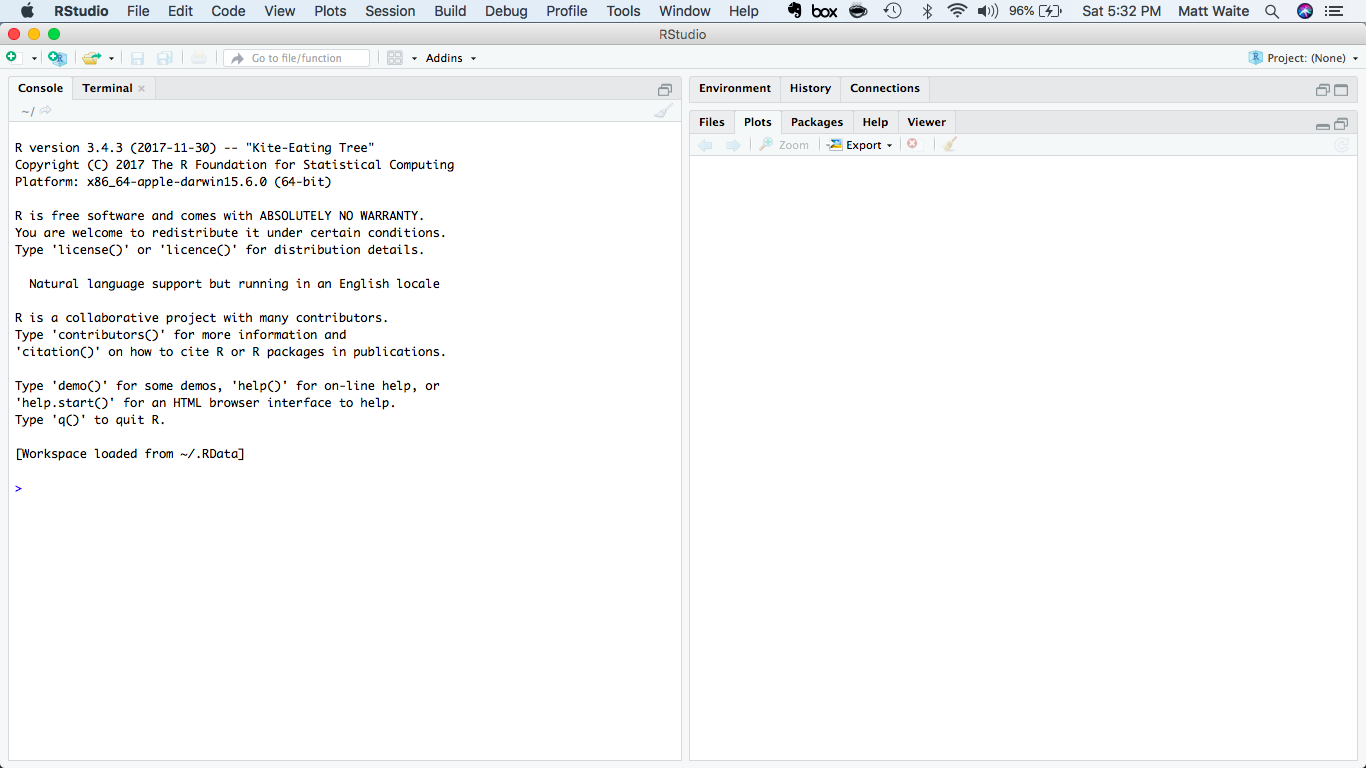
\includegraphics[width=18.97in]{images/verybasics1}

Think of the console like talking directly to R. It's direct, but it has
some drawbacks and some quirks we'll get into later. For now, try typing
this into the console and hit enter:

\begin{Shaded}
\begin{Highlighting}[]
\DecValTok{2}\OperatorTok{+}\DecValTok{2}
\end{Highlighting}
\end{Shaded}

\begin{verbatim}
## [1] 4
\end{verbatim}

Congrats, you've run some code. It's not very complex, and you knew the
answer before hand, but you get the idea. We can compute things. We can
also store things. In programming languages, these are called variables
or objects. We can assign things to variables using
\texttt{\textless{}-}. And then we can do things with them. Try this in
your console.

\begin{Shaded}
\begin{Highlighting}[]
\NormalTok{number <-}\StringTok{ }\DecValTok{2}

\NormalTok{number }\OperatorTok{*}\StringTok{ }\NormalTok{number}
\end{Highlighting}
\end{Shaded}

\begin{verbatim}
## [1] 4
\end{verbatim}

We can have as many variables as we can name. We can even reuse them
(but be careful you know you're doing that or you'll introduce errors).
Try this in your console.

\begin{Shaded}
\begin{Highlighting}[]
\NormalTok{firstnumber <-}\StringTok{ }\DecValTok{1}
\NormalTok{secondnumber <-}\DecValTok{2} 

\NormalTok{(firstnumber }\OperatorTok{+}\StringTok{ }\NormalTok{secondnumber) }\OperatorTok{*}\StringTok{ }\NormalTok{secondnumber}
\end{Highlighting}
\end{Shaded}

\begin{verbatim}
## [1] 6
\end{verbatim}

We can store anything in a variable. A whole table. An array of numbers.
A single word. A whole book. All the books of the 18th century. They're
really powerful. We'll exlore them at length.

\section{Adding libraries, part 1}\label{adding-libraries-part-1}

The real strength of any given programming language is the external
libraries that power it. The base language can do a lot, but it's the
external libraries that solve many specific problems -- even making the
base language easier to use.

For this class, we're going to need several external libraries.

The first library we're going to use is called Swirl. So in the console,
type
\texttt{install.packages(\textquotesingle{}swirl\textquotesingle{})} and
hit enter. That installs swirl.

Now, to use the library, type \texttt{library(swirl)} and hit enter.
That loads swirl. Then type \texttt{swirl()} and hit enter. Now you're
running swirl. Follow the directions on the screen. When you are asked,
you want to install course 1 R Programming: The basics of programming in
R. Then, when asked, you want to do option 1, R Programming, in that
course.

When you are finished with the course -- it will take just a few minutes
-- type 0 to exit (it will not be clear that's what you do when you are
done).

\section{Adding libraries, part 2}\label{adding-libraries-part-2}

We'll mostly use two libraries for analysis -- \texttt{dplyr} and
\texttt{ggplot2}. To get them, and several other useful libraries, we
can install a single collection of libraries called the tidyverse. Type
this into your console:
\texttt{install.packages(\textquotesingle{}tidyverse\textquotesingle{})}

\textbf{NOTE}: This is a pattern. You should always install libraries in
the console.

Then, to help us with learning and replication, we're going to use R
Notebooks. So we need to install that library. Type this into your
console:
\texttt{install.packages(\textquotesingle{}rmarkdown\textquotesingle{})}

\section{Notebooks}\label{notebooks}

For the rest of the class, we're going to be working in notebooks. In
notebooks, you will both run your code and explain each step, much as I
am doing here.

To start a notebook, you click on the green plus in the top left corner
and go down to R Notebook. Do that now.

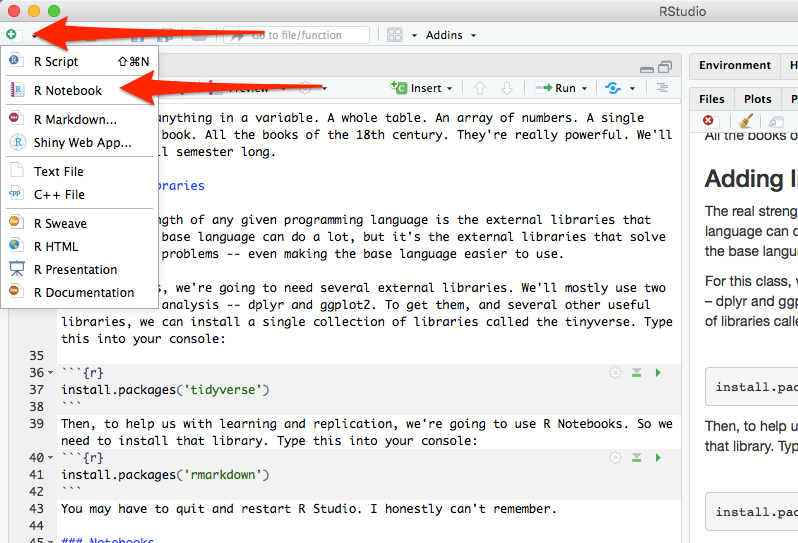
\includegraphics[width=11.08in]{images/verybasics2}

You will see that the notebook adds a lot of text for you. It tells you
how to work in notebooks -- and you should read it. The most important
parts are these:

To add text, simply type. To add code you can click on the \emph{Insert}
button on the toolbar or by pressing \emph{Cmd+Option+I} on Mac or
\emph{Ctl+Option+I} on Windows.

Highlight all that text and delete it. You should have a blank document.
This document is called a R Markdown file -- it's a special form of
text, one that you can style, and one you can include R in the middle of
it. Markdown is a simple markup format that you can use to create
documents. So first thigns first, let's give our notebook a big
headline. Add this:

\texttt{\#\ My\ awesome\ notebook}

Now, under that, without any markup, just type This is my awesome
notebook.

Under that, you can make text bold by writing
\texttt{It\ is\ **really**\ awesome}.

If you want it italics, just do this on the next line:
\texttt{No,\ it\textquotesingle{}s\ \_really\_\ awesome.\ I\ swear.}

To see what it looks like without the markup, click the Preview or Knit
button in the toolbar. That will turn you notebook into a webpage, with
the formatting included.

Throughout this book, we're going to use this markdown to explain what
we are doing and, more importantly, why we are doing it. Explaining your
thinking is a vital part of understanding what you are doing.

That explaination, plus the code, is the real power of notebooks. To add
a block of code, follow the instructions from above: click on the
\emph{Insert} button on the toolbar or by pressing \emph{Cmd+Option+I}
on Mac or \emph{Ctl+Option+I} on Windows.

In that window, use some of the code from above and add two numbers
together. To see it run, click the green triangle on the right. That
runs the chunk. You should see the answer to your addition problem.

And that, just that, is the foundation you need to start this book.

\chapter{Data, structures and types}\label{data-structures-and-types}

Data are everywhere (and data is plural of datum, thus the use of are in
that statement). It surrounds you. Every time you use your phone, you
are creating data. Lots of it. Your online life. Any time you buy
something. It's everywhere. Sports, like life, is no different. Sports
is drowning in data, and more comes along all the time.

In sports, and in this class, we'll be dealing largely with two kinds of
data: event level data and summary data. It's not hard to envision event
level data in sports. A pitch in baseball. A hit. A play in football. A
pass in soccer. They are the events that make up the game. Combine them
together -- summarize them -- and you'll have some notion of how the
game went. What we usually see is summary data -- who wants to scroll
through 50 pitches to find out a player went 2-3 with a double and an
RBI? Who wants to scroll through hundreds of pitches to figure out the
Rays beat the Yankees?

To start with, we need to understand the shape of data.

\begin{quote}
EXERCISE: Try scoring a child's board game. For example, Chutes and
Ladders. If you were placed in charge of analytics for the World Series
of Chutes and Ladders, what is your event level data? What summary data
do you keep? If you've got the game, try it.
\end{quote}

\section{Rows and columns}\label{rows-and-columns}

Data, oversimplifying it a bit, is information organized. Generally
speaking, it's organized into rows and columns. Rows, generally, are
individual elements. A team. A player. A game. Columns, generally, are
components of the data, sometimes called variables. So if each row is a
player, the first column might be their name. The second is their
position. The third is their batting average. And so on.

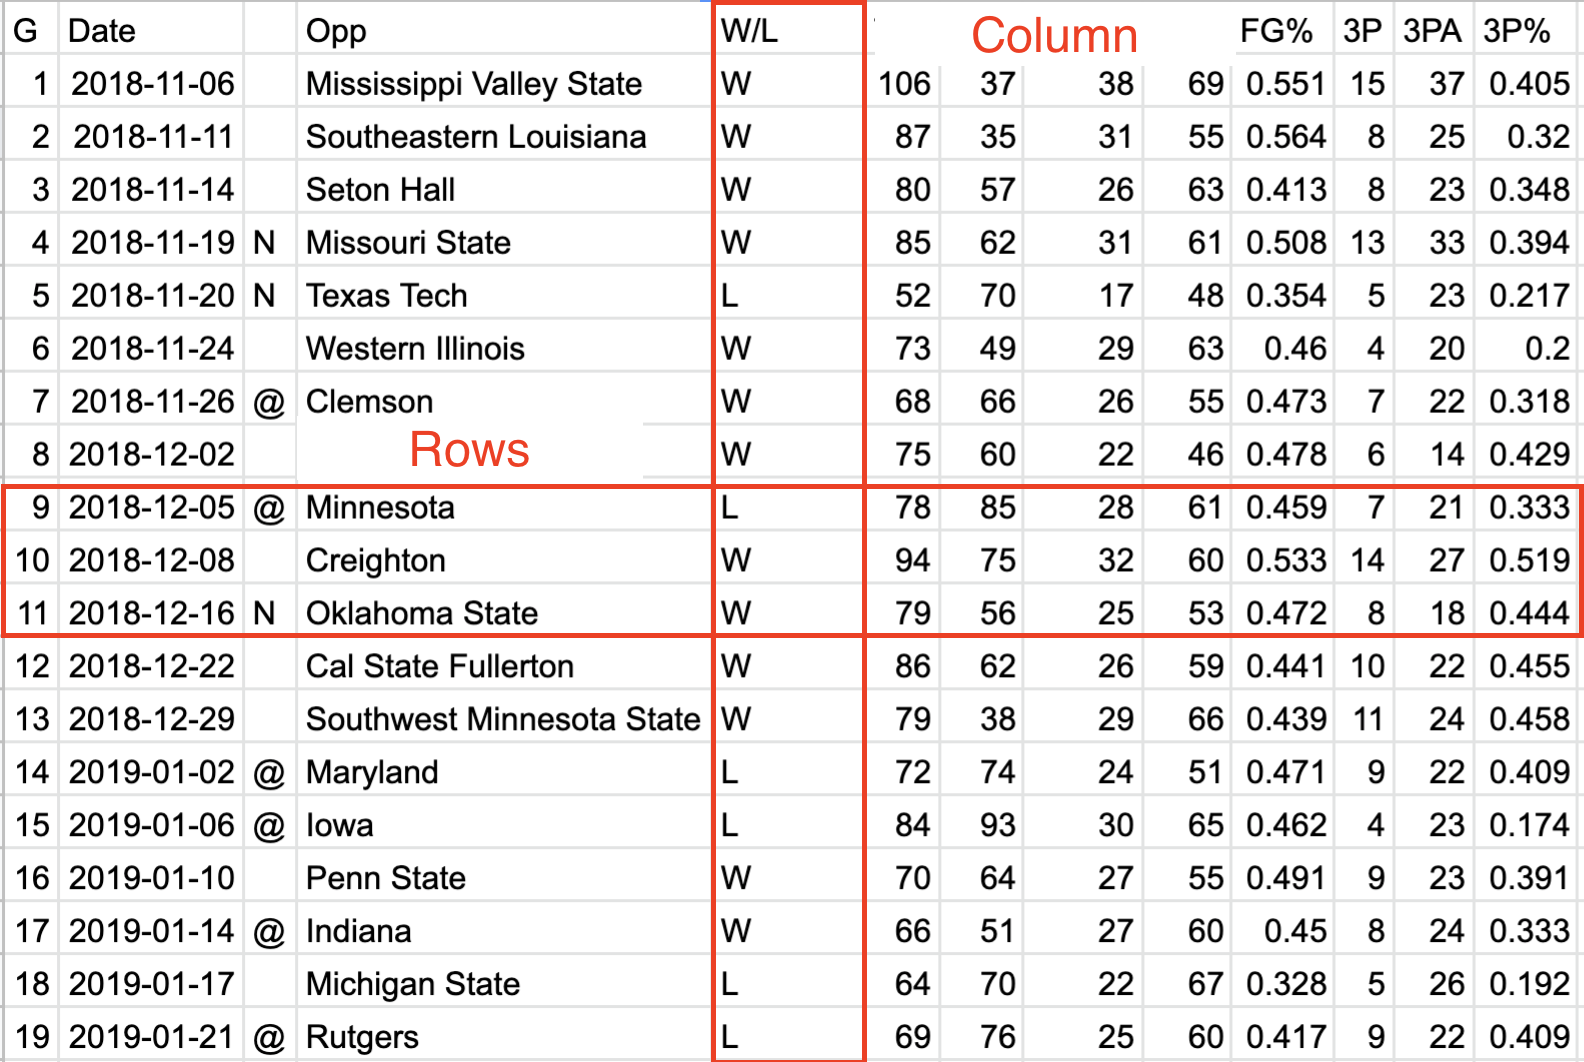
\includegraphics[width=22in]{images/data1}

One of the critical components of data analysis, especially for
beginners, is having a mental picture of your data. What does each row
mean? What does each column in each row signify? How many rows do you
have? How many columns?

\section{A simple way to get data}\label{a-simple-way-to-get-data}

One good thing about sports is that there's lots of interest in it. And
that means there's outlets that put sports data on the internet. Now I'm
going to show you a trick to getting it easily.

The site sports-reference.com takes NCAA (and other league) stats and
puts them online. For instance,
\href{https://www.sports-reference.com/cbb/schools/nebraska/2019-gamelogs.html}{here's
their page on Nebraska basketball's game logs}, which you should open
now.

Now, in a new tab, log into Google Docs/Drive and open a new
spreadsheet. In the first cell of the first row, copy and paste this
formula in:

\begin{verbatim}
=IMPORTHTML("https://www.sports-reference.com/cbb/schools/nebraska/2019-gamelogs.html", "table", 1)
\end{verbatim}

If it worked right, you've got the data from that page in a spreadsheet.

\section{Cleaning the data}\label{cleaning-the-data}

The first thing we need to do is recognize that we don't have data,
really. We have the results of a formula. You can tell by putting your
cursor on that field, where you'll see the formula again. This is where
you'd look:

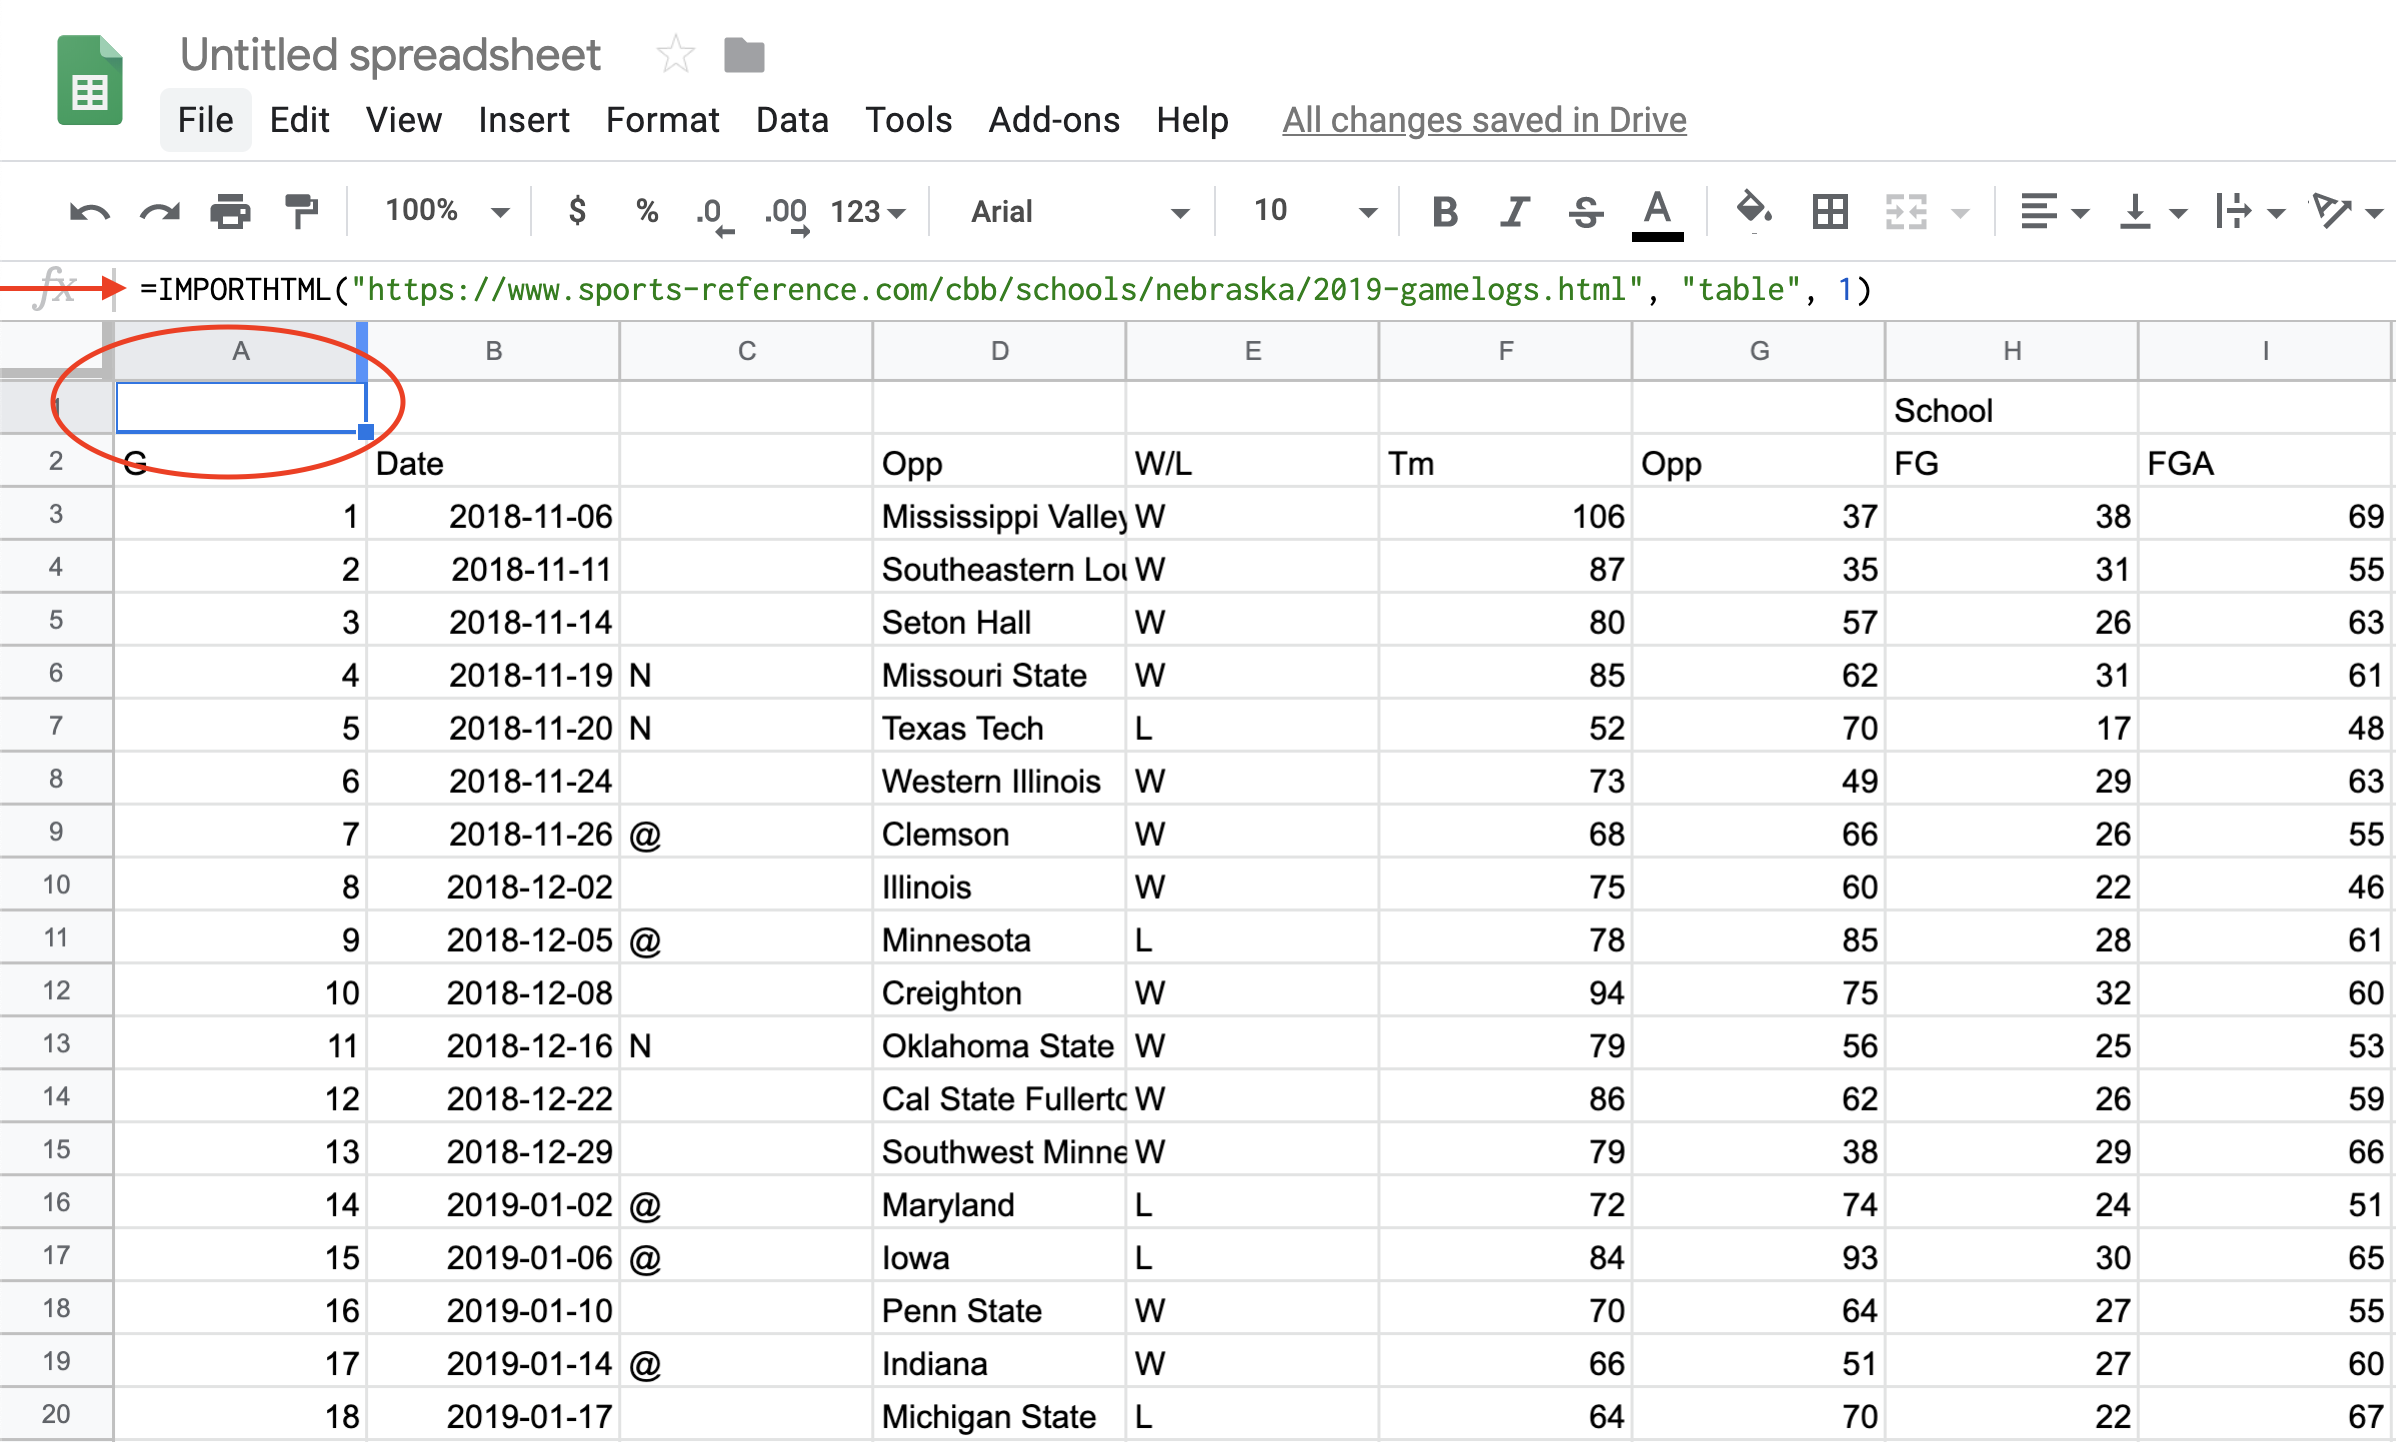
\includegraphics[width=33.28in]{images/clean1}

The solution is easy:

Edit \textgreater{} Select All or type command/control A Edit
\textgreater{} Copy or type command/control c Edit \textgreater{} Paste
Special \textgreater{} Values Only or type command/control shift v

You can verify that it worked by looking in that same row 1 column A,
where you'll see the formula is gone.

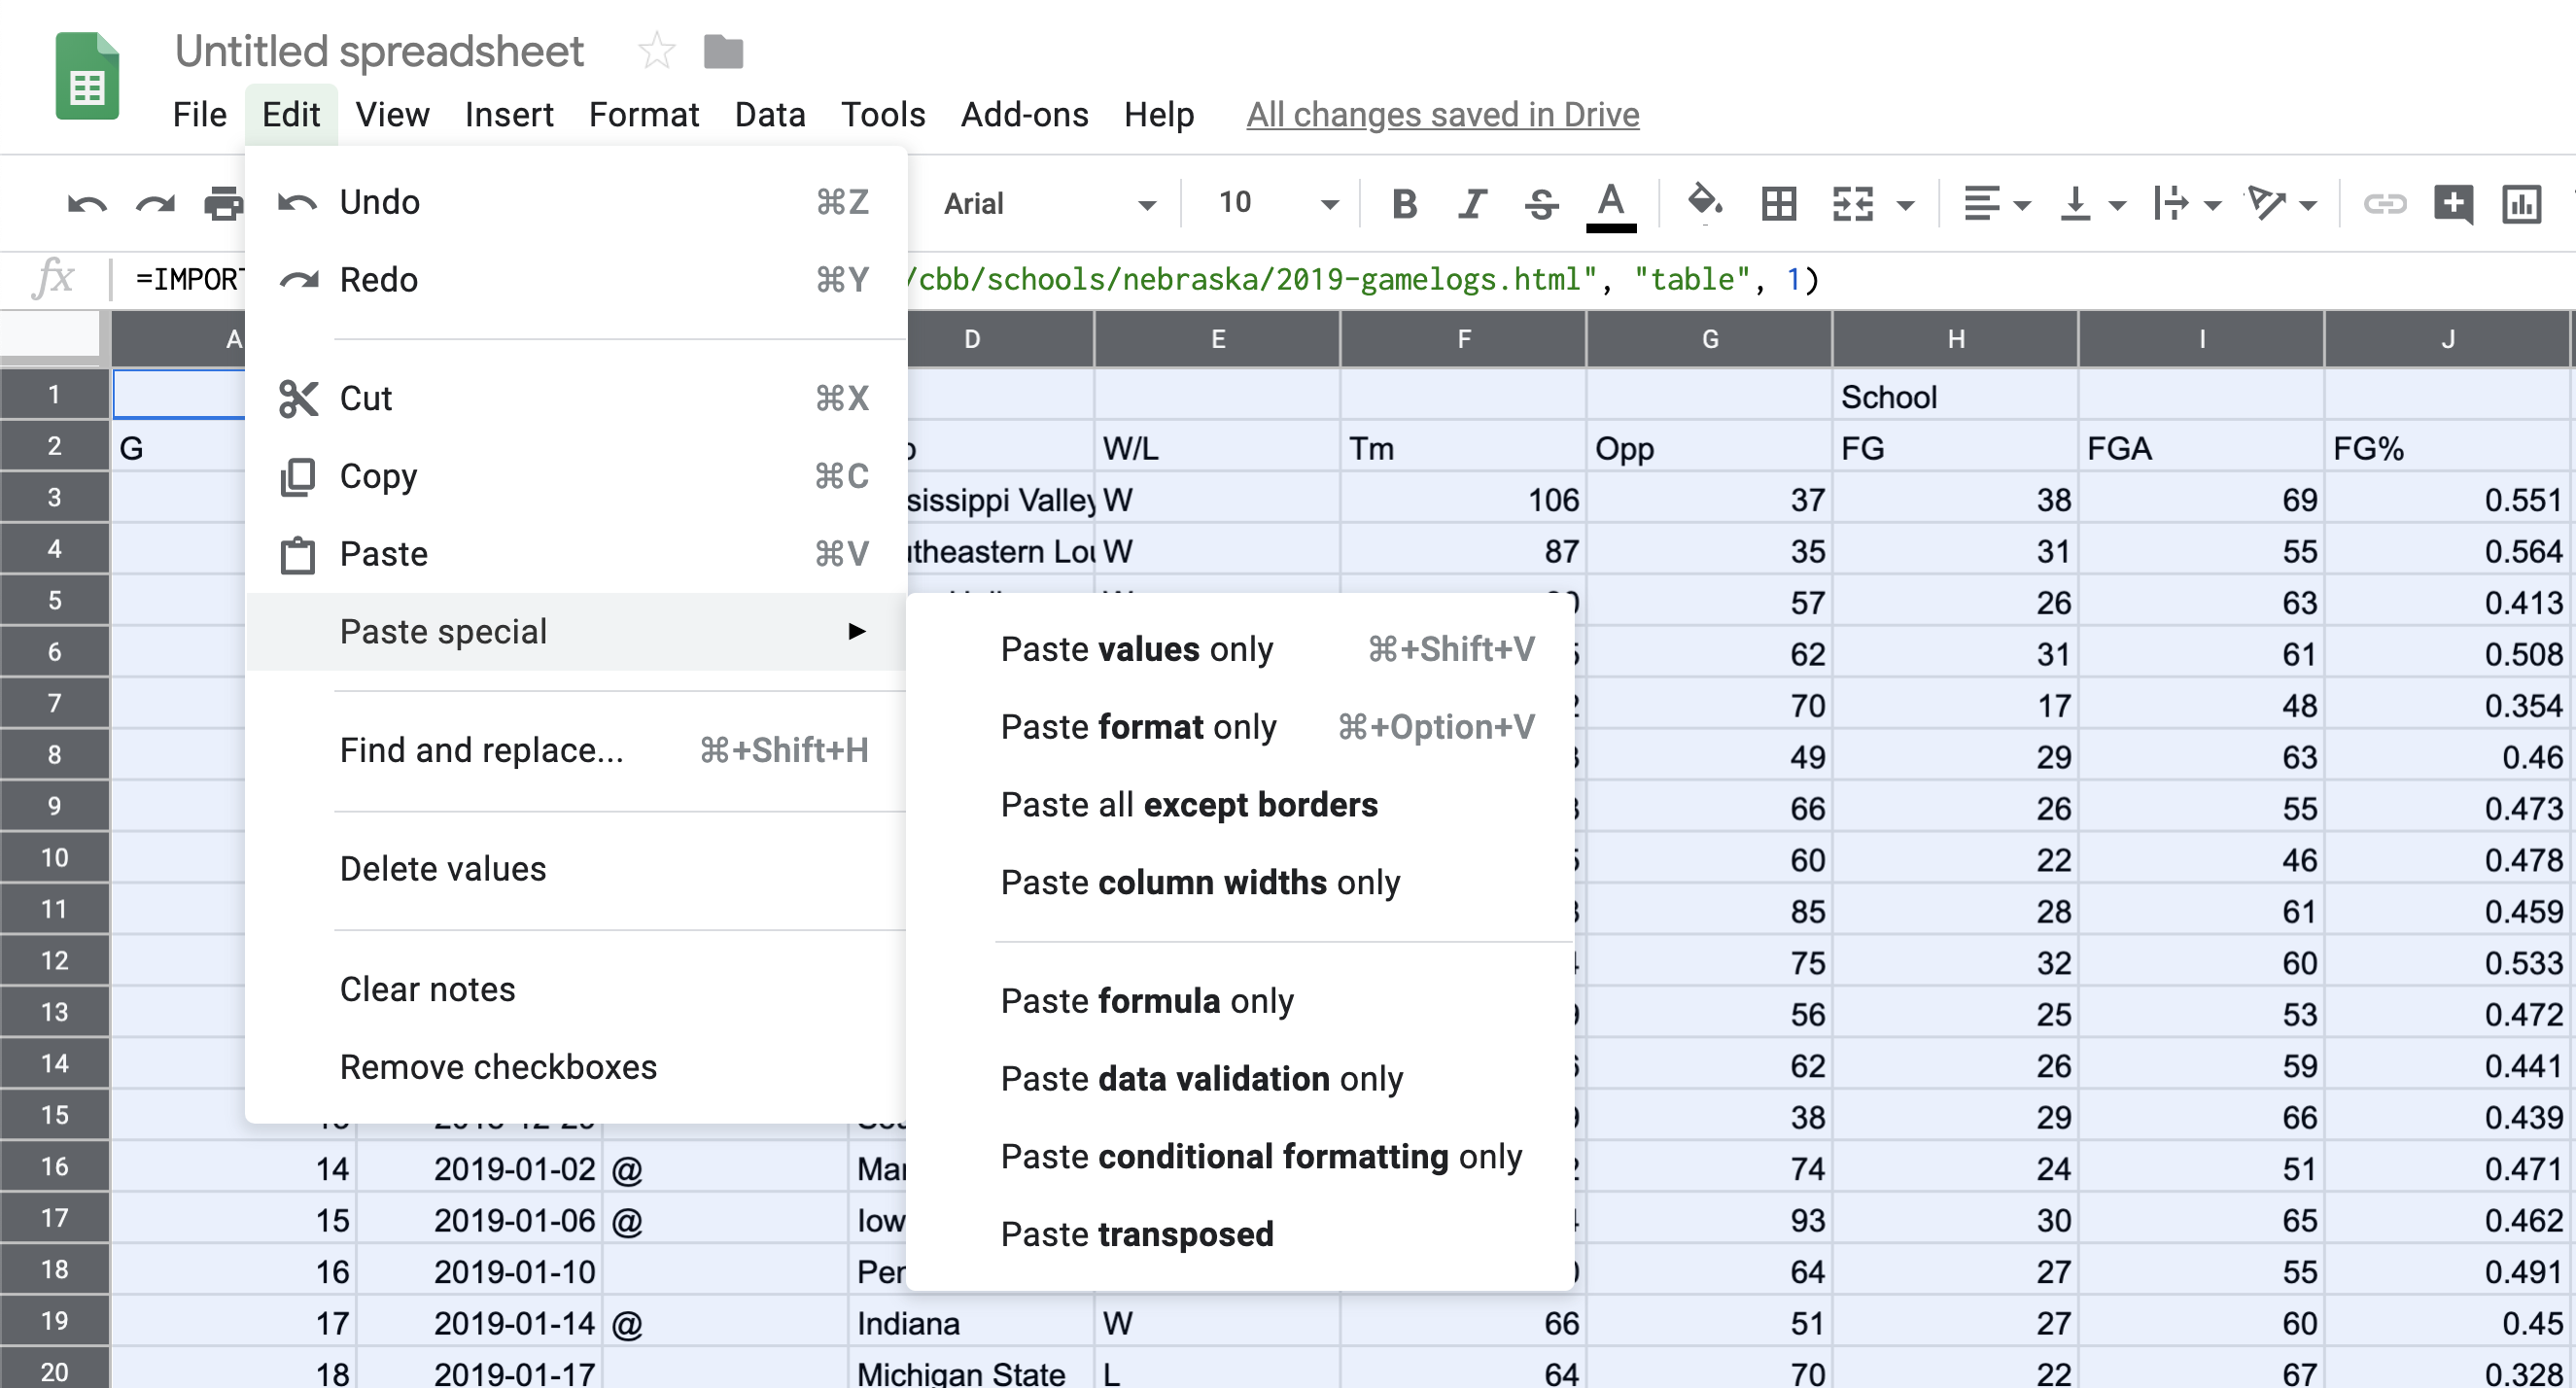
\includegraphics[width=36.81in]{images/clean2}

Now you have data, but your headers are all wrong. You want your headers
to be one line -- not two, like they have. And the header names repeat
-- first for our team, then for theirs. So you have to change each
header name to be UsORB or TeamORB and OpponentORB instead of just ORB.

After you've done that, note we have repeating headers. There's two ways
to deal with that -- you could just hightlight it and go up to Edit
\textgreater{} Delete Rows XX-XX depending on what rows you highlighted.
That's the easy way with our data.

But what if you had hundreds of repeating headers like that? Deleting
them would take a long time.

You can use sorting to get rid of anything that's not data. So click on
Data \textgreater{} Sort Range. You'll want to check the ``Data has
header row'' field. Then hit Sort.

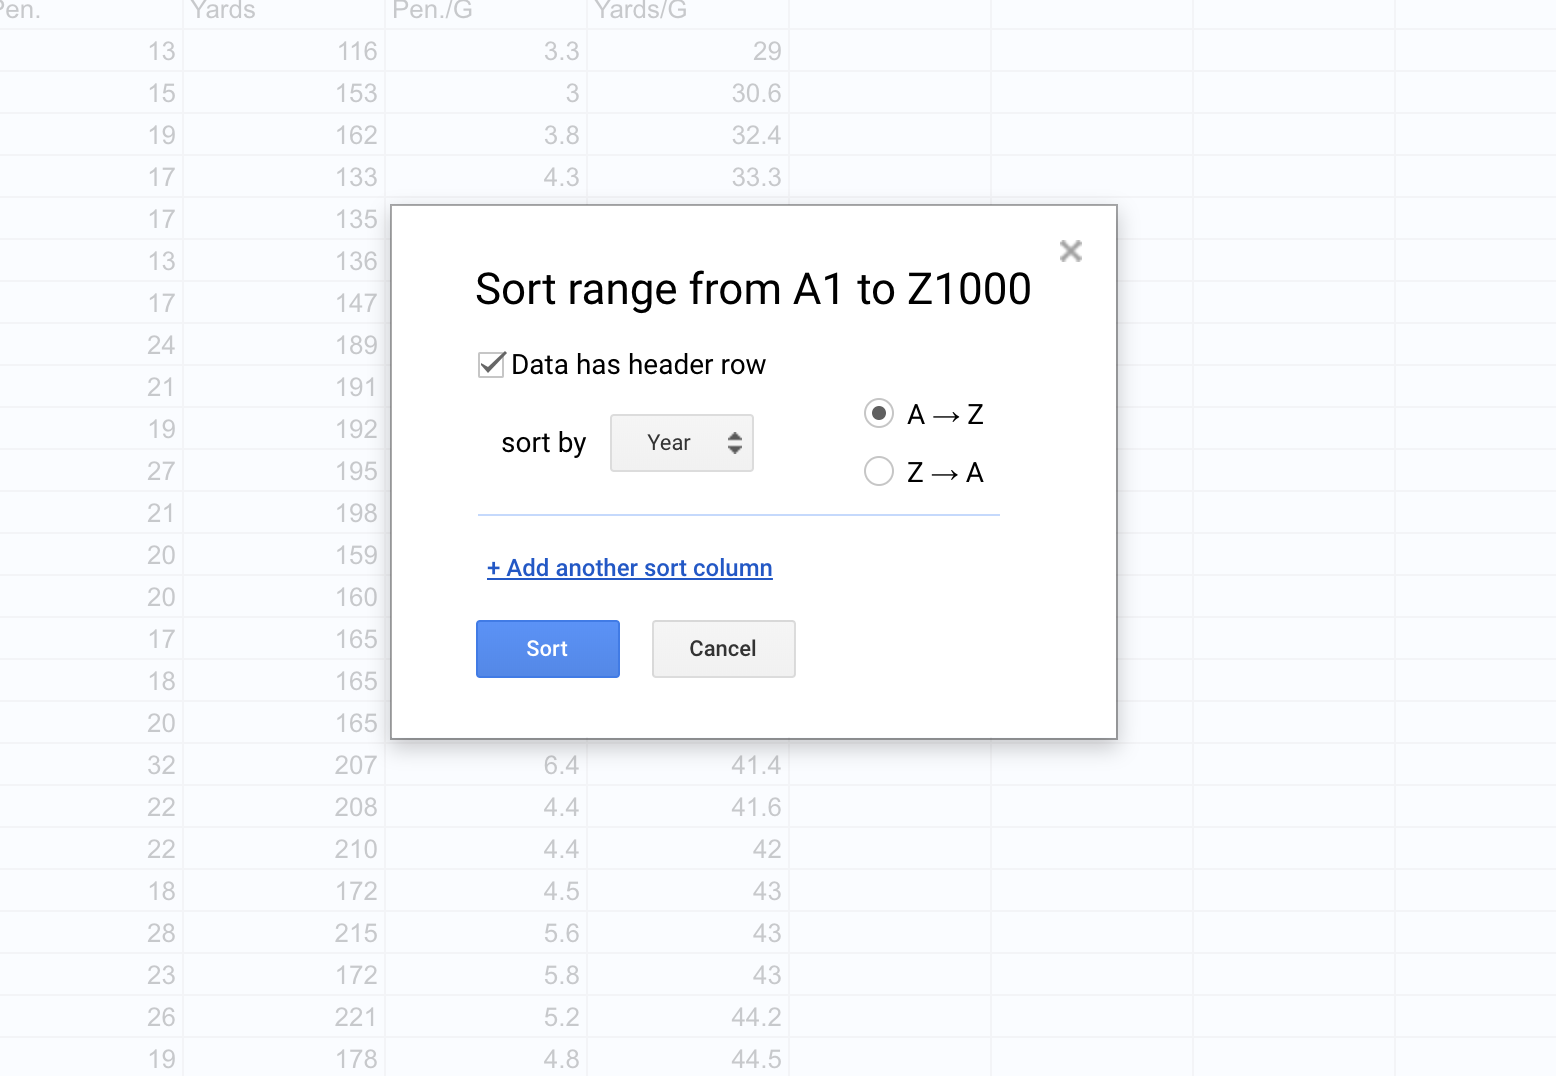
\includegraphics[width=21.61in]{images/clean3}

Now all you need to do is search through the data for where your junk
data -- extra headers, blanks, etc. -- got sorted and delete it. After
you've done that, you can export it for use in R. Go to File
\textgreater{} Download as \textgreater{} Comma Separated Values.
Remember to put it in the same directory as your R Notebook file so you
can import the data easily.

\chapter{Aggregates}\label{aggregates}

R is a statistical programming language that is purpose built for data
analysis.

Base R does a lot, but there are a mountain of external libraries that
do things to make R better/easier/more fully featured. We already
installed the tidyverse -- or you should have if you followed the
instructions for the last assignment -- which isn't exactly a library,
but a collection of libraries. Together, they make up the tidyverse.
Individually, they are extraordinarily useful for what they do. We can
load them all at once using the tidyverse name, or we can load them
individually. Let's start with individually.

The two libraries we are going to need for this assignement are
\texttt{readr} and \texttt{dplyr}. The library \texttt{readr} reads
different types of data in. For this assignment, we're going to read in
csv data or Comma Separated Values data. That's data that has a comma
between each column of data.

Then we're going to use \texttt{dplyr} to analyze it.

To use a library, you need to import it. Good practice -- one I'm going
to insist on -- is that you put all your library steps at the top of
your notebooks.

That code looks like this:

\begin{Shaded}
\begin{Highlighting}[]
\KeywordTok{library}\NormalTok{(readr)}
\end{Highlighting}
\end{Shaded}

To load them both, you need to run that code twice:

\begin{Shaded}
\begin{Highlighting}[]
\KeywordTok{library}\NormalTok{(readr)}
\KeywordTok{library}\NormalTok{(dplyr)}
\end{Highlighting}
\end{Shaded}

You can keep doing that for as many libraries as you need. I've seen
notebooks with 10 or more library imports.

\section{Basic data analysis: Group By and
Count}\label{basic-data-analysis-group-by-and-count}

The first thing we need to do is get some data to work with. We do that
by reading it in. In our case, we're going to read data from a csv file
-- a comma-separated values file.

The CSV file we're going to read from is a
\href{https://unl.box.com/s/xjipgkesl9rjmng4weg77vb73xt41apf}{Nebraska
Game and Parks Commission dataset} of confirmed mountain lion sightings
in Nebraska. There are, on occasion, fierce debates about mountain lions
and if they should be hunted in Nebraska. This dataset can tell us some
interesting things about that debate.

So step 1 is to import the data. The code looks \emph{something} like
this, but hold off copying it just yet:

\texttt{mountainlions\ \textless{}-\ read\_csv("\textasciitilde{}/Documents/Data/mountainlions.csv")}

Let's unpack that.

The first part -- mountainlions -- is the name of your variable. A
variable is just a name of a thing. In this case, our variable is a data
frame, which is R's way of storing data. We can call this whatever we
want. I always want to name data frames after what is in it. In this
case, we're going to import a dataset of mountain lion sightings from
the Nebraska Game and Parks Commission. Variable names, by convention
are one word all lower case. You can end a variable with a number, but
you can't start one with a number.

The \textless{}- bit is the variable assignment operator. It's how we
know we're assigning something to a word. Think of the arrow as saying
``Take everything on the right of this arrow and stuff it into the thing
on the left.'' So we're creating an empty vessel called mountainlions
and stuffing all this data into it.

The \texttt{read\_csv} bits are pretty obvious, except for one thing.
What happens in the quote marks is the path to the data. In there, I
have to tell R where it will find the data. The easiest thing to do, if
you are confused about how to find your data, is to put your data in the
same folder as as your notebook (you'll have to save that notebook
first). If you do that, then you just need to put the name of the file
in there (mountainlions.csv). In my case, I've got a folder called
Documents in my home directory (that's the \texttt{\textasciitilde{}}
part), and in there is a folder called Data that has the file called
mountainlions.csv in it. Some people -- insane people -- leave the data
in their downloads folder. The data path then would be
\texttt{\textasciitilde{}/Downloads/nameofthedatafilehere.csv} on PC or
Mac.

\textbf{What you put in there will be different from mine}. So your
first task is to import the data.

\begin{Shaded}
\begin{Highlighting}[]
\NormalTok{mountainlions <-}\StringTok{ }\KeywordTok{read_csv}\NormalTok{(}\StringTok{"data/mountainlions.csv"}\NormalTok{)}
\end{Highlighting}
\end{Shaded}

\begin{verbatim}
## Parsed with column specification:
## cols(
##   ID = col_double(),
##   `Cofirm Type` = col_character(),
##   COUNTY = col_character(),
##   Date = col_character()
## )
\end{verbatim}

Now we can inspect the data we imported. What does it look like? To do
that, we use \texttt{head(mountainlions)} to show the headers and the
first six rows of data. If we wanted to see them all, we could just
simply enter \texttt{mountainlions} and run it.

To get the number of records in our dataset, we run
\texttt{nrow(mountainlions)}

\begin{Shaded}
\begin{Highlighting}[]
\KeywordTok{head}\NormalTok{(mountainlions)}
\end{Highlighting}
\end{Shaded}

\begin{verbatim}
## # A tibble: 6 x 4
##      ID `Cofirm Type` COUNTY       Date    
##   <dbl> <chr>         <chr>        <chr>   
## 1     1 Track         Dawes        9/14/91 
## 2     2 Mortality     Sioux        11/10/91
## 3     3 Mortality     Scotts Bluff 4/21/96 
## 4     4 Mortality     Sioux        5/9/99  
## 5     5 Mortality     Box Butte    9/29/99 
## 6     6 Track         Scotts Bluff 11/12/99
\end{verbatim}

\begin{Shaded}
\begin{Highlighting}[]
\KeywordTok{nrow}\NormalTok{(mountainlions)}
\end{Highlighting}
\end{Shaded}

\begin{verbatim}
## [1] 393
\end{verbatim}

So what if we wanted to know how many mountain lion sightings there were
in each county? To do that by hand, we'd have to take each of the 393
records and sort them into a pile. We'd put them in groups and then
count them.

\texttt{dplyr} has a group by function in it that does just this. A
massive amount of data analysis involves grouping like things together
at some point. So it's a good place to start.

So to do this, we'll take our dataset and we'll introduce a new
operator: \%\textgreater{}\%. The best way to read that operator, in my
opinion, is to interpret that as ``and then do this.'' Here's the code:

\begin{Shaded}
\begin{Highlighting}[]
\NormalTok{mountainlions }\OperatorTok
\StringTok{  }\KeywordTok{group_by}\NormalTok{(COUNTY) }\OperatorTok
\StringTok{  }\KeywordTok{summarise}\NormalTok{(}
    \DataTypeTok{total =} \KeywordTok{n}\NormalTok{()}
\NormalTok{  )}
\end{Highlighting}
\end{Shaded}

\begin{verbatim}
## # A tibble: 42 x 2
##    COUNTY    total
##    <chr>     <int>
##  1 Banner        6
##  2 Blaine        3
##  3 Box Butte     4
##  4 Brown        15
##  5 Buffalo       3
##  6 Cedar         1
##  7 Cherry       30
##  8 Custer        8
##  9 Dakota        3
## 10 Dawes       111
## # ... with 32 more rows
\end{verbatim}

So let's walk through that. We start with our dataset --
\texttt{mountainlions} -- and then we tell it to group the data by a
given field in the data. In this case, we wanted to group together all
the counties, signified by the field name COUNTY, which you could get
from looking at \texttt{head(mountainlions)}. After we group the data,
we need to count them up. In dplyr, we use \texttt{summarize}
\href{http://dplyr.tidyverse.org/reference/summarise.html}{which can do
more than just count things}. Inside the parentheses in summarize, we
set up the summaries we want. In this case, we just want a count of the
counties: \texttt{count\ =\ n(),} says create a new field, called
\texttt{total} and set it equal to \texttt{n()}, which might look weird,
but it's common in stats. The number of things in a dataset?
Statisticians call in n. There are n number of incidents in this
dataset. So \texttt{n()} is a function that counts the number of things
there are.

And when we run that, we get a list of counties with a count next to
them. But it's not in any order. So we'll add another And Then Do This
\%\textgreater{}\% and use \texttt{arrange}. Arrange does what you think
it does -- it arranges data in order. By default, it's in ascending
order -- smallest to largest. But if we want to know the county with the
most mountain lion sightings, we need to sort it in descending order.
That looks like this:

\begin{Shaded}
\begin{Highlighting}[]
\NormalTok{mountainlions }\OperatorTok
\StringTok{  }\KeywordTok{group_by}\NormalTok{(COUNTY) }\OperatorTok
\StringTok{  }\KeywordTok{summarise}\NormalTok{(}
    \DataTypeTok{count =} \KeywordTok{n}\NormalTok{()}
\NormalTok{  ) }\OperatorTok\StringTok{ }\KeywordTok{arrange}\NormalTok{(}\KeywordTok{desc}\NormalTok{(count))}
\end{Highlighting}
\end{Shaded}

\begin{verbatim}
## # A tibble: 42 x 2
##    COUNTY       count
##    <chr>        <int>
##  1 Dawes          111
##  2 Sioux           52
##  3 Sheridan        35
##  4 Cherry          30
##  5 Scotts Bluff    26
##  6 Keya Paha       20
##  7 Brown           15
##  8 Rock            11
##  9 Lincoln         10
## 10 Custer           8
## # ... with 32 more rows
\end{verbatim}

We can, if we want, group by more than one thing. So how are these
sightings being confirmed? To do that, we can group by County and
``Cofirm Type'', which is how the state misspelled Confirm. But note
something in this example below:

\begin{Shaded}
\begin{Highlighting}[]
\NormalTok{mountainlions }\OperatorTok
\StringTok{  }\KeywordTok{group_by}\NormalTok{(COUNTY, }\StringTok{`}\DataTypeTok{Cofirm Type}\StringTok{`}\NormalTok{) }\OperatorTok
\StringTok{  }\KeywordTok{summarise}\NormalTok{(}
    \DataTypeTok{count =} \KeywordTok{n}\NormalTok{()}
\NormalTok{  ) }\OperatorTok\StringTok{ }\KeywordTok{arrange}\NormalTok{(}\KeywordTok{desc}\NormalTok{(count))}
\end{Highlighting}
\end{Shaded}

\begin{verbatim}
## # A tibble: 93 x 3
## # Groups:   COUNTY [42]
##    COUNTY       `Cofirm Type`      count
##    <chr>        <chr>              <int>
##  1 Dawes        Trail Camera Photo    41
##  2 Sioux        Trail Camera Photo    40
##  3 Dawes        Track                 19
##  4 Keya Paha    Trail Camera Photo    18
##  5 Cherry       Trail Camera Photo    17
##  6 Dawes        Mortality             17
##  7 Sheridan     Trail Camera Photo    16
##  8 Dawes        Photo                 13
##  9 Dawes        DNA                   11
## 10 Scotts Bluff Trail Camera Photo    11
## # ... with 83 more rows
\end{verbatim}

See it? When you have a field name that has two words, \texttt{readr}
wraps it in backticks, which is next to the 1 key on your keyboard. You
can figure out which fields have backticks around it by looking at the
output of \texttt{readr}. Pay attention to that, because it's coming up
again in the next section and will be a part of your homework.

\section{Other aggregates: Mean and
median}\label{other-aggregates-mean-and-median}

In the last example, we grouped some data together and counted it up,
but there's so much more you can do. You can do multiple measures in a
single step as well.

Let's look at some
\href{https://unl.box.com/s/09t2u4qoncfh6qlv2156flzlxb8ruzpq}{salary
data from the University of Nebraska}.

\begin{Shaded}
\begin{Highlighting}[]
\NormalTok{salaries <-}\StringTok{ }\KeywordTok{read_csv}\NormalTok{(}\StringTok{"data/nusalaries1819.csv"}\NormalTok{)}
\end{Highlighting}
\end{Shaded}

\begin{verbatim}
## Parsed with column specification:
## cols(
##   Employee = col_character(),
##   Position = col_character(),
##   Campus = col_character(),
##   Department = col_character(),
##   `Budgeted Annual Salary` = col_number(),
##   `Salary from State Aided Funds` = col_number(),
##   `Salary from Other Funds` = col_number()
## )
\end{verbatim}

\begin{Shaded}
\begin{Highlighting}[]
\KeywordTok{head}\NormalTok{(salaries)}
\end{Highlighting}
\end{Shaded}

\begin{verbatim}
## # A tibble: 6 x 7
##   Employee Position Campus Department `Budgeted Annua~ `Salary from St~
##   <chr>    <chr>    <chr>  <chr>                 <dbl>            <dbl>
## 1 Abbey, ~ Associa~ UNK    Kinesiolo~            61276            61276
## 2 Abbott,~ Staff S~ UNL    FM&P Faci~            37318               NA
## 3 Abboud,~ Adminis~ UNMC   Surgery-U~            76400            76400
## 4 Abdalla~ Asst Pr~ UNMC   Pathology~            74774            71884
## 5 Abdelka~ Post-Do~ UNMC   Surgery-T~            43516               NA
## 6 Abdel-M~ Researc~ UNL    Public Po~            58502               NA
## # ... with 1 more variable: `Salary from Other Funds` <dbl>
\end{verbatim}

In summarize, we can calculate any number of measures. Here, we'll use
R's built in mean and median functions to calculate \ldots{} well, you
get the idea.

\begin{Shaded}
\begin{Highlighting}[]
\NormalTok{salaries }\OperatorTok
\StringTok{  }\KeywordTok{summarise}\NormalTok{(}
    \DataTypeTok{count =} \KeywordTok{n}\NormalTok{(),}
    \DataTypeTok{mean_salary =} \KeywordTok{mean}\NormalTok{(}\StringTok{`}\DataTypeTok{Budgeted Annual Salary}\StringTok{`}\NormalTok{),}
    \DataTypeTok{median_salary =} \KeywordTok{median}\NormalTok{(}\StringTok{`}\DataTypeTok{Budgeted Annual Salary}\StringTok{`}\NormalTok{)}
\NormalTok{  )}
\end{Highlighting}
\end{Shaded}

\begin{verbatim}
## # A tibble: 1 x 3
##   count mean_salary median_salary
##   <int>       <dbl>         <dbl>
## 1 13039      62065.         51343
\end{verbatim}

So there's 13,039 employees in the database, spread across four campuses
plus the system office. The mean or average salary is about \$62,000,
but the median salary is slightly more than \$51,000.

Why?

Let's let sort help us.

\begin{Shaded}
\begin{Highlighting}[]
\NormalTok{salaries }\OperatorTok\StringTok{ }\KeywordTok{arrange}\NormalTok{(}\KeywordTok{desc}\NormalTok{(}\StringTok{`}\DataTypeTok{Budgeted Annual Salary}\StringTok{`}\NormalTok{))}
\end{Highlighting}
\end{Shaded}

\begin{verbatim}
## # A tibble: 13,039 x 7
##    Employee Position Campus Department `Budgeted Annua~ `Salary from St~
##    <chr>    <chr>    <chr>  <chr>                 <dbl>            <dbl>
##  1 Frost, ~ Head Co~ UNL    Athletics           5000000               NA
##  2 Miles, ~ Head Co~ UNL    Athletics           2375000               NA
##  3 Moos, W~ Athleti~ UNL    Athletics           1000000               NA
##  4 Gold, J~ Chancel~ UNMC   Office of~           853338           853338
##  5 Chinand~ Assista~ UNL    Athletics            800000               NA
##  6 Walters~ Assista~ UNL    Athletics            700000               NA
##  7 Cook, J~ Head Co~ UNL    Athletics            675000               NA
##  8 William~ Head Co~ UNL    Athletics            626750               NA
##  9 Bounds,~ Preside~ UNCA   Office of~           540000           540000
## 10 Austin ~ Assista~ UNL    Athletics            475000               NA
## # ... with 13,029 more rows, and 1 more variable: `Salary from Other
## #   Funds` <dbl>
\end{verbatim}

Oh, right. In this dataset, the university pays a football coach \$5
million. Extremes influence averages, not medians, and now you have your
answer.

So when choosing a measure of the middle, you have to ask yourself --
could I have extremes? Because a median won't be sensitive to extremes.
It will be the point at which half the numbers are above and half are
below. The average or mean will be a measure of the middle, but if you
have a bunch of low paid people and then one football coach, the average
will be wildly skewed. Here, because there's so few highly paid football
coaches compared to people who make a normal salary, the number is only
slightly skewed in the grand scheme, but skewed nonetheless.

\chapter{Mutating data}\label{mutating-data}

One of the most common data analysis techniques is to look at change
over time. The most common way of comparing change over time is through
percent change. The math behind calculating percent change is very
simple, and you should know it off the top of your head. The easy way to
remember it is:

\texttt{(new\ -\ old)\ /\ old}

Or new minus old divided by old. Your new number minus the old number,
the result of which is divided by the old number. To do that in R, we
can use \texttt{dplyr} and \texttt{mutate} to calculate new metrics in a
new field using existing fields of data.

So first we'll import the tidyverse so we can read in our data and begin
to work with it.

\begin{Shaded}
\begin{Highlighting}[]
\KeywordTok{library}\NormalTok{(tidyverse)}
\end{Highlighting}
\end{Shaded}

Now we'll import a common and
\href{https://unl.box.com/s/hvxmnxhr41x4ikgt3vk38aczcbrf97pn}{simple
dataset of total attendance} at NCAA football games over the last few
seasons.

\begin{Shaded}
\begin{Highlighting}[]
\NormalTok{attendance <-}\StringTok{ }\KeywordTok{read_csv}\NormalTok{(}\StringTok{'data/attendance.csv'}\NormalTok{)}
\end{Highlighting}
\end{Shaded}

\begin{verbatim}
## Parsed with column specification:
## cols(
##   Institution = col_character(),
##   Conference = col_character(),
##   `2013` = col_double(),
##   `2014` = col_double(),
##   `2015` = col_double(),
##   `2016` = col_double(),
##   `2017` = col_double(),
##   `2018` = col_double()
## )
\end{verbatim}

\begin{Shaded}
\begin{Highlighting}[]
\KeywordTok{head}\NormalTok{(attendance)}
\end{Highlighting}
\end{Shaded}

\begin{verbatim}
## # A tibble: 6 x 8
##   Institution     Conference      `2013` `2014` `2015` `2016` `2017` `2018`
##   <chr>           <chr>            <dbl>  <dbl>  <dbl>  <dbl>  <dbl>  <dbl>
## 1 Air Force       MWC             228562 168967 156158 177519 174924 166205
## 2 Akron           MAC             107101  55019 108588  62021 117416  92575
## 3 Alabama         SEC             710538 710736 707786 712747 712053 710931
## 4 Appalachian St. FBS Independent 149366     NA     NA     NA     NA     NA
## 5 Appalachian St. Sun Belt            NA 138995 128755 156916 154722 131716
## 6 Arizona         Pac-12          285713 354973 308355 338017 255791 318051
\end{verbatim}

The code to calculate percent change is pretty simple. Remember, with
\texttt{summarize}, we used \texttt{n()} to count things. With
\texttt{mutate}, we use very similar syntax to calculate a new value
using other values in our dataset. So in this case, we're trying to do
(new-old)/old, but we're doing it with fields. If we look at what we got
when we did \texttt{head}, you'll see there's `2018` as the new data,
and we'll use `2017` as the old data. So we're looking at one year.
Then, to help us, we'll use arrange again to sort it, so we get the
fastest growing school over one year.

\begin{Shaded}
\begin{Highlighting}[]
\NormalTok{attendance }\OperatorTok\StringTok{ }\KeywordTok{mutate}\NormalTok{(}
  \DataTypeTok{change =}\NormalTok{ (}\StringTok{`}\DataTypeTok{2018}\StringTok{`} \OperatorTok{-}\StringTok{ `}\DataTypeTok{2017}\StringTok{`}\NormalTok{)}\OperatorTok{/}\StringTok{`}\DataTypeTok{2017}\StringTok{`}
\NormalTok{) }
\end{Highlighting}
\end{Shaded}

\begin{verbatim}
## # A tibble: 150 x 9
##    Institution Conference `2013` `2014` `2015` `2016` `2017` `2018`
##    <chr>       <chr>       <dbl>  <dbl>  <dbl>  <dbl>  <dbl>  <dbl>
##  1 Air Force   MWC        228562 168967 156158 177519 174924 166205
##  2 Akron       MAC        107101  55019 108588  62021 117416  92575
##  3 Alabama     SEC        710538 710736 707786 712747 712053 710931
##  4 Appalachia~ FBS Indep~ 149366     NA     NA     NA     NA     NA
##  5 Appalachia~ Sun Belt       NA 138995 128755 156916 154722 131716
##  6 Arizona     Pac-12     285713 354973 308355 338017 255791 318051
##  7 Arizona St. Pac-12     501509 343073 368985 286417 359660 291091
##  8 Arkansas    SEC        431174 399124 471279 487067 442569 367748
##  9 Arkansas S~ Sun Belt   149477 149163 138043 136200 119538 119001
## 10 Army West ~ FBS Indep~ 169781 171310 185946 163267 185543 190156
## # ... with 140 more rows, and 1 more variable: change <dbl>
\end{verbatim}

What do we see right away? Do those numbers look like we expect them to?
No. They're a decimal expressed as a percentage. So let's fix that by
multiplying by 100.

\begin{Shaded}
\begin{Highlighting}[]
\NormalTok{attendance }\OperatorTok\StringTok{ }\KeywordTok{mutate}\NormalTok{(}
  \DataTypeTok{change =}\NormalTok{ ((}\StringTok{`}\DataTypeTok{2018}\StringTok{`} \OperatorTok{-}\StringTok{ `}\DataTypeTok{2017}\StringTok{`}\NormalTok{)}\OperatorTok{/}\StringTok{`}\DataTypeTok{2017}\StringTok{`}\NormalTok{)}\OperatorTok{*}\DecValTok{100}
\NormalTok{) }
\end{Highlighting}
\end{Shaded}

\begin{verbatim}
## # A tibble: 150 x 9
##    Institution Conference `2013` `2014` `2015` `2016` `2017` `2018`  change
##    <chr>       <chr>       <dbl>  <dbl>  <dbl>  <dbl>  <dbl>  <dbl>   <dbl>
##  1 Air Force   MWC        228562 168967 156158 177519 174924 166205  -4.98 
##  2 Akron       MAC        107101  55019 108588  62021 117416  92575 -21.2  
##  3 Alabama     SEC        710538 710736 707786 712747 712053 710931  -0.158
##  4 Appalachia~ FBS Indep~ 149366     NA     NA     NA     NA     NA  NA    
##  5 Appalachia~ Sun Belt       NA 138995 128755 156916 154722 131716 -14.9  
##  6 Arizona     Pac-12     285713 354973 308355 338017 255791 318051  24.3  
##  7 Arizona St. Pac-12     501509 343073 368985 286417 359660 291091 -19.1  
##  8 Arkansas    SEC        431174 399124 471279 487067 442569 367748 -16.9  
##  9 Arkansas S~ Sun Belt   149477 149163 138043 136200 119538 119001  -0.449
## 10 Army West ~ FBS Indep~ 169781 171310 185946 163267 185543 190156   2.49 
## # ... with 140 more rows
\end{verbatim}

Now, does this ordering do anything for us? No. Let's fix that with
arrange.

\begin{Shaded}
\begin{Highlighting}[]
\NormalTok{attendance }\OperatorTok\StringTok{ }\KeywordTok{mutate}\NormalTok{(}
  \DataTypeTok{change =}\NormalTok{ ((}\StringTok{`}\DataTypeTok{2018}\StringTok{`} \OperatorTok{-}\StringTok{ `}\DataTypeTok{2017}\StringTok{`}\NormalTok{)}\OperatorTok{/}\StringTok{`}\DataTypeTok{2017}\StringTok{`}\NormalTok{)}\OperatorTok{*}\DecValTok{100}
\NormalTok{) }\OperatorTok\StringTok{ }\KeywordTok{arrange}\NormalTok{(}\KeywordTok{desc}\NormalTok{(change))}
\end{Highlighting}
\end{Shaded}

\begin{verbatim}
## # A tibble: 150 x 9
##    Institution  Conference `2013` `2014` `2015` `2016` `2017` `2018` change
##    <chr>        <chr>       <dbl>  <dbl>  <dbl>  <dbl>  <dbl>  <dbl>  <dbl>
##  1 Ga. Southern Sun Belt       NA 105510 124681 104095  61031 100814   65.2
##  2 La.-Monroe   Sun Belt    85177  90540  58659  67057  49640  71048   43.1
##  3 Louisiana    Sun Belt   129878 154652 129577 121346  78754 111303   41.3
##  4 Hawaii       MWC        185931 192159 164031 170299 145463 205455   41.2
##  5 Buffalo      MAC        136418 122418 110743 104957  80102 110280   37.7
##  6 California   Pac-12     345303 286051 292797 279769 219290 300061   36.8
##  7 UCF          AAC        252505 226869 180388 214814 257924 352148   36.5
##  8 UTSA         C-USA      175282 165458 138048 138226 114104 148257   29.9
##  9 Eastern Mic~ MAC         20255  75127  29381 106064  73649  95632   29.8
## 10 Louisville   ACC            NA 317829 294413 324391 276957 351755   27.0
## # ... with 140 more rows
\end{verbatim}

So who had the most growth last year from the year before? Something
going on at Georgia Southern.

\section{A more complex example}\label{a-more-complex-example}

There's metric in basketball that's easy to understand -- shooting
percentage. It's the number of shots made divided by the number of shots
attempted. Simple, right? Except it's a little too simple. Because what
about three point shooters? They tend to be more vailable because the
three point shot is worth more. What about players who get to the line?
In shooting percentage, free throws are nowhere to be found.

Basketball nerds, because of these weaknesses, have created a new metric
called
\href{https://en.wikipedia.org/wiki/True_shooting_percentage}{True
Shooting Percentage}. True shooting percentage takes into account all
aspects of a players shooting to determine who the real shooters are.

Using \texttt{dplyr} and \texttt{mutate}, we can calculate true shooting
percentage. So let's look at a new dataset, one of
\href{https://unl.box.com/s/s1wzw61u9ia50qmirfhuvprgpmmah9rj}{every
college basketball player's season stats in 2018-19 season}. It's a
dataset of 5,386 players, and we've got 59 variables -- one of them is
True Shooting Percentage, but we're going to ignore that.

\begin{Shaded}
\begin{Highlighting}[]
\NormalTok{players <-}\StringTok{ }\KeywordTok{read_csv}\NormalTok{(}\StringTok{"data/players19.csv"}\NormalTok{)}
\end{Highlighting}
\end{Shaded}

\begin{verbatim}
## Warning: Missing column names filled in: 'X1' [1]
\end{verbatim}

\begin{verbatim}
## Parsed with column specification:
## cols(
##   .default = col_double(),
##   Team = col_character(),
##   Conference = col_character(),
##   Player = col_character(),
##   Class = col_character(),
##   Pos = col_character(),
##   Height = col_character(),
##   Hometown = col_character(),
##   `High School` = col_character(),
##   Summary = col_character()
## )
\end{verbatim}

\begin{verbatim}
## See spec(...) for full column specifications.
\end{verbatim}

The basic true shooting percentage formula is
\texttt{(Points\ /\ (2*(FieldGoalAttempts\ +\ (.44\ *\ FreeThrowAttempts))))\ *\ 100}.
Let's talk that through. Points divided by a lot. It's really field goal
attempts plus 44 percent of the free throw attempts. Why? Because that's
about what a free throw is worth, compared to other ways to score. After
adding those things together, you double it. And after you divide points
by that number, you multiply the whole lot by 100.

In our data, we need to be able to find the fields so we can complete
the formula. To do that, one way is to use the Environment tab in R
Studio. In the Environment tab is a listing of all the data you've
imported, and if you click the triangle next to it, it'll list all the
field names, giving you a bit of information about each one.

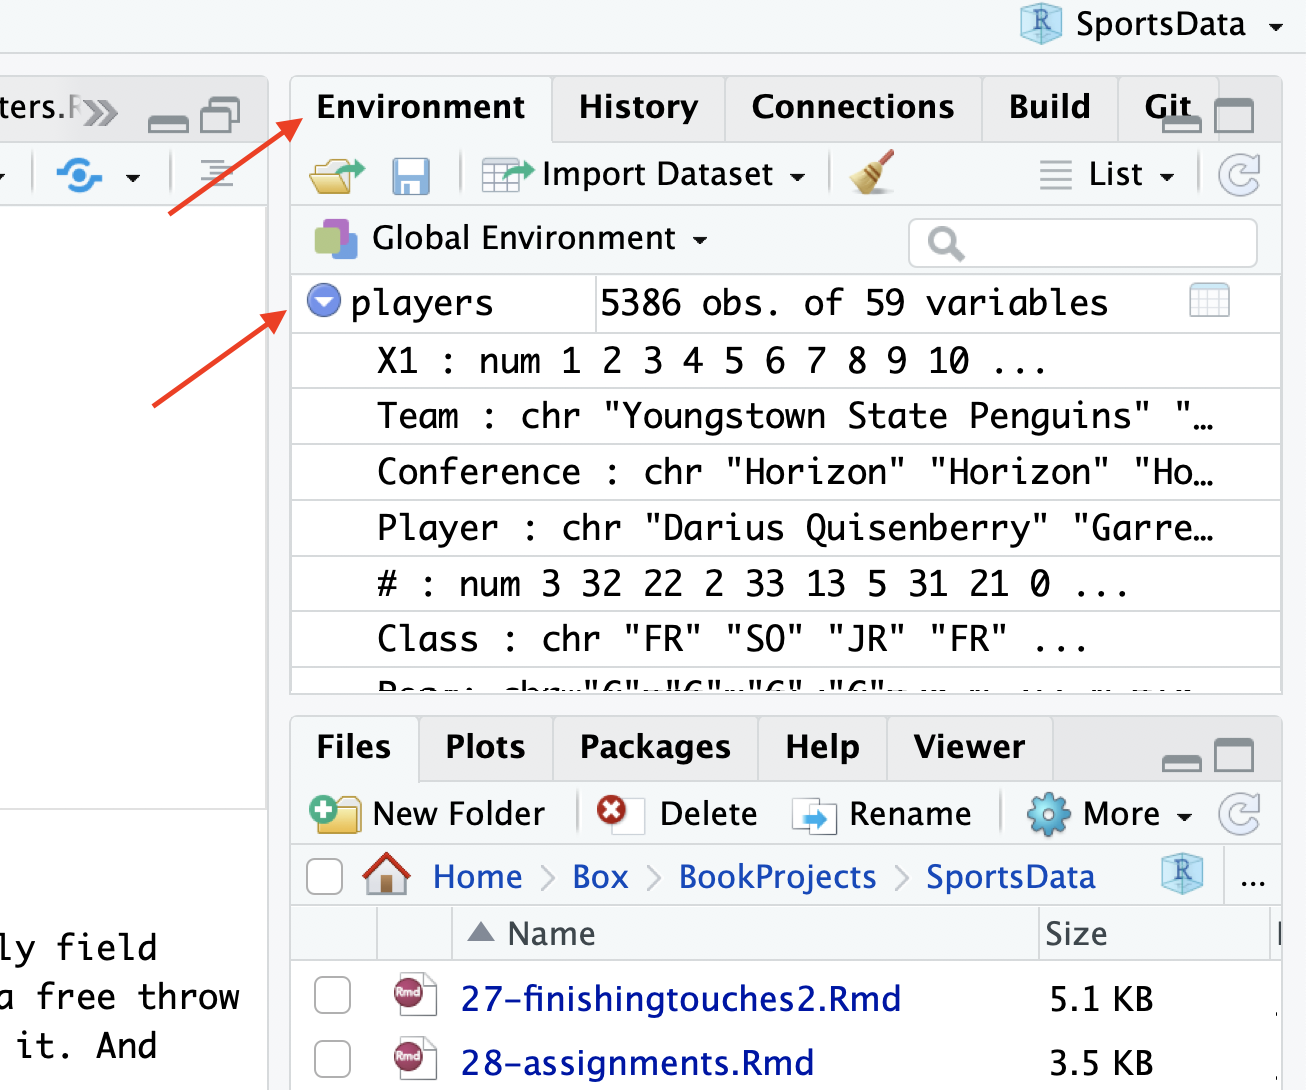
\includegraphics[width=18.14in]{images/environment}

So what does True Shooting Percentage look like in code?

Let's think about this differently. Who had the best true shooting
season last year?

\begin{Shaded}
\begin{Highlighting}[]
\NormalTok{players }\OperatorTok
\StringTok{  }\KeywordTok{mutate}\NormalTok{(}\DataTypeTok{trueshooting =}\NormalTok{ (PTS}\OperatorTok{/}\NormalTok{(}\DecValTok{2}\OperatorTok{*}\NormalTok{(FGA }\OperatorTok{+}\StringTok{ }\NormalTok{(.}\DecValTok{44}\OperatorTok{*}\NormalTok{FTA))))}\OperatorTok{*}\DecValTok{100}\NormalTok{) }\OperatorTok
\StringTok{  }\KeywordTok{arrange}\NormalTok{(}\KeywordTok{desc}\NormalTok{(trueshooting))}
\end{Highlighting}
\end{Shaded}

\begin{verbatim}
## # A tibble: 5,386 x 60
##       X1 Team  Conference Player   `#` Class Pos   Height Weight Hometown
##    <dbl> <chr> <chr>      <chr>  <dbl> <chr> <chr> <chr>   <dbl> <chr>   
##  1   579 Texa~ Big 12     Drayt~     4 JR    G     6-0       156 Austin,~
##  2   843 Ston~ AEC        Nick ~    42 FR    F     6-7       240 Port Je~
##  3  1059 Sout~ Southland  Patri~    22 SO    F     6-3       210 Folsom,~
##  4  4269 Dayt~ A-10       Camro~    52 SO    G     5-7       160 Country~
##  5  4681 Cali~ Pac-12     David~    21 JR    G     6-4       185 Newbury~
##  6   326 Virg~ ACC        Grant~     1 FR    G     <NA>       NA Charlot~
##  7   410 Vand~ SEC        Mac H~    42 FR    G     6-6       182 Chattan~
##  8  1390 Sain~ A-10       Jack ~    31 JR    G     6-6       205 Mattoon~
##  9  2230 NJIT~ A-Sun      Patri~     3 SO    G     5-9       160 West Or~
## 10   266 Wash~ Pac-12     Reaga~    34 FR    F     6-6       225 Santa A~
## # ... with 5,376 more rows, and 50 more variables: `High School` <chr>,
## #   Summary <chr>, Rk.x <dbl>, G <dbl>, GS <dbl>, MP <dbl>, FG <dbl>,
## #   FGA <dbl>, `FG%` <dbl>, `2P` <dbl>, `2PA` <dbl>, `2P%` <dbl>,
## #   `3P` <dbl>, `3PA` <dbl>, `3P%` <dbl>, FT <dbl>, FTA <dbl>,
## #   `FT%` <dbl>, ORB <dbl>, DRB <dbl>, TRB <dbl>, AST <dbl>, STL <dbl>,
## #   BLK <dbl>, TOV <dbl>, PF <dbl>, PTS <dbl>, Rk.y <dbl>, PER <dbl>,
## #   `TS%` <dbl>, `eFG%` <dbl>, `3PAr` <dbl>, FTr <dbl>, PProd <dbl>,
## #   `ORB%` <dbl>, `DRB%` <dbl>, `TRB%` <dbl>, `AST%` <dbl>, `STL%` <dbl>,
## #   `BLK%` <dbl>, `TOV%` <dbl>, `USG%` <dbl>, OWS <dbl>, DWS <dbl>,
## #   WS <dbl>, `WS/40` <dbl>, OBPM <dbl>, DBPM <dbl>, BPM <dbl>,
## #   trueshooting <dbl>
\end{verbatim}

You'll be forgiven if you did not hear about Texas Longhorns shooting
sensation Drayton Whiteside. He played in six games, took one shot and
actually hit it. It happened to be a three pointer, which is one more
three pointer than I've hit in college basketball. So props to him. Does
that mean he had the best true shooting season in college basketball
last year? Not hardly.

We'll talk about how to narrow the pile and filter out data in the next
chapter.

\chapter{Filters and selections}\label{filters-and-selections}

More often than not, we have more data than we want. Sometimes we need
to be rid of that data. In \texttt{dplyr}, there's two ways to go about
this: filtering and selecting.

\textbf{Filtering creates a subset of the data based on criteria}. All
records where the count is greater than 10. All records that match
``Nebraska''. Something like that.

\textbf{Selecting simply returns only the fields named}. So if you only
want to see School and Attendance, you select those fields. When you
look at your data again, you'll have two columns. If you try to use one
of your columns that you had before you used select, you'll get an
error.

Let's work with our football attendance data to show some examples.

\begin{Shaded}
\begin{Highlighting}[]
\KeywordTok{library}\NormalTok{(tidyverse)}
\end{Highlighting}
\end{Shaded}

\begin{Shaded}
\begin{Highlighting}[]
\NormalTok{attendance <-}\StringTok{ }\KeywordTok{read_csv}\NormalTok{(}\StringTok{'data/attendance.csv'}\NormalTok{)}
\end{Highlighting}
\end{Shaded}

\begin{verbatim}
## Parsed with column specification:
## cols(
##   Institution = col_character(),
##   Conference = col_character(),
##   `2013` = col_double(),
##   `2014` = col_double(),
##   `2015` = col_double(),
##   `2016` = col_double(),
##   `2017` = col_double(),
##   `2018` = col_double()
## )
\end{verbatim}

So, first things first, let's say we don't care about all this Air
Force, Akron, Alabama crap and just want to see Dear Old Nebraska U. We
do that with \texttt{filter} and then we pass it a condition.

Before we do that, a note about conditions. Most of the conditional
operators you'll understand -- greater than and less than are
\textgreater{} and \textless{}. The tough one to remember is equal to.
In conditional statements, equal to is == not =. If you haven't noticed,
= is a variable assignment operator, not a conditional statement. So
equal is == and NOT equal is !=.

So if you want to see Institutions equal to Nebraska, you do this:

\begin{Shaded}
\begin{Highlighting}[]
\NormalTok{attendance }\OperatorTok\StringTok{ }\KeywordTok{filter}\NormalTok{(Institution }\OperatorTok{==}\StringTok{ "Nebraska"}\NormalTok{)}
\end{Highlighting}
\end{Shaded}

\begin{verbatim}
## # A tibble: 1 x 8
##   Institution Conference `2013` `2014` `2015` `2016` `2017` `2018`
##   <chr>       <chr>       <dbl>  <dbl>  <dbl>  <dbl>  <dbl>  <dbl>
## 1 Nebraska    Big Ten    727466 638744 629983 631402 628583 623240
\end{verbatim}

Or if we want to see schools that had more than half a million people
buy tickets to a football game in a season, we do the following. NOTE
THE BACKTICKS.

\begin{Shaded}
\begin{Highlighting}[]
\NormalTok{attendance }\OperatorTok\StringTok{ }\KeywordTok{filter}\NormalTok{(}\StringTok{`}\DataTypeTok{2018}\StringTok{`} \OperatorTok{>=}\StringTok{ }\DecValTok{500000}\NormalTok{)}
\end{Highlighting}
\end{Shaded}

\begin{verbatim}
## # A tibble: 17 x 8
##    Institution    Conference `2013` `2014` `2015` `2016` `2017` `2018`
##    <chr>          <chr>       <dbl>  <dbl>  <dbl>  <dbl>  <dbl>  <dbl>
##  1 Alabama        SEC        710538 710736 707786 712747 712053 710931
##  2 Auburn         SEC        685252 612157 612157 695498 605120 591236
##  3 Clemson        ACC        574333 572262 588266 566787 565412 562799
##  4 Florida        SEC        524638 515001 630457 439229 520290 576299
##  5 Georgia        SEC        556476 649222 649222 556476 556476 649222
##  6 LSU            SEC        639927 712063 654084 708618 591034 705733
##  7 Michigan       Big Ten    781144 734364 771174 883741 669534 775156
##  8 Michigan St.   Big Ten    506294 522765 522628 522666 507398 508088
##  9 Nebraska       Big Ten    727466 638744 629983 631402 628583 623240
## 10 Ohio St.       Big Ten    734528 744075 750705 750944 752464 713630
## 11 Oklahoma       Big 12     508334 510972 512139 521142 519119 607146
## 12 Penn St.       Big Ten    676112 711358 698590 701800 746946 738396
## 13 South Carolina SEC        576805 569664 472934 538441 550099 515396
## 14 Tennessee      SEC        669087 698276 704088 706776 670454 650887
## 15 Texas          Big 12     593857 564618 540210 587283 556667 586277
## 16 Texas A&M      SEC        697003 630735 725354 713418 691612 698908
## 17 Wisconsin      Big Ten    552378 556642 546099 476144 551766 540072
\end{verbatim}

But what if we want to see all of the Power Five conferences? We
\emph{could} use conditional logic in our filter. The conditional logic
operators are \texttt{\textbar{}} for OR and \texttt{\&} for AND. NOTE:
AND means all conditions have to be met. OR means any of the conditions
work. So be careful about boolean logic.

\begin{Shaded}
\begin{Highlighting}[]
\NormalTok{attendance }\OperatorTok\StringTok{ }\KeywordTok{filter}\NormalTok{(Conference }\OperatorTok{==}\StringTok{ "Big 10"} \OperatorTok{|}\StringTok{ }\NormalTok{Conference }\OperatorTok{==}\StringTok{ "SEC"} \OperatorTok{|}\StringTok{ }\NormalTok{Conference }\OperatorTok{==}\StringTok{ "Pac-12"} \OperatorTok{|}\StringTok{ }\NormalTok{Conference }\OperatorTok{==}\StringTok{ "ACC"} \OperatorTok{|}\StringTok{ }\NormalTok{Conference }\OperatorTok{==}\StringTok{ "Big 12"}\NormalTok{)}
\end{Highlighting}
\end{Shaded}

\begin{verbatim}
## # A tibble: 51 x 8
##    Institution    Conference `2013` `2014` `2015` `2016` `2017` `2018`
##    <chr>          <chr>       <dbl>  <dbl>  <dbl>  <dbl>  <dbl>  <dbl>
##  1 Alabama        SEC        710538 710736 707786 712747 712053 710931
##  2 Arizona        Pac-12     285713 354973 308355 338017 255791 318051
##  3 Arizona St.    Pac-12     501509 343073 368985 286417 359660 291091
##  4 Arkansas       SEC        431174 399124 471279 487067 442569 367748
##  5 Auburn         SEC        685252 612157 612157 695498 605120 591236
##  6 Baylor         Big 12     321639 280257 276960 275029 262978 248017
##  7 Boston College ACC        198035 239893 211433 192942 215546 263363
##  8 California     Pac-12     345303 286051 292797 279769 219290 300061
##  9 Clemson        ACC        574333 572262 588266 566787 565412 562799
## 10 Colorado       Pac-12     230778 226670 236331 279652 282335 274852
## # ... with 41 more rows
\end{verbatim}

But that's a lot of repetitive code. And a lot of typing. And typing is
the devil. So what if we could create a list and pass it into the
filter? It's pretty simple.

We can create a new variable -- remember variables can represent just
about anything -- and create a list. To do that we use the \texttt{c}
operator, which stands for concatenate. That just means take all the
stuff in the parenthesis after the c and bunch it into a list.

Note here: text is in quotes. If they were numbers, we wouldn't need the
quotes.

\begin{Shaded}
\begin{Highlighting}[]
\NormalTok{powerfive <-}\StringTok{ }\KeywordTok{c}\NormalTok{(}\StringTok{"SEC"}\NormalTok{, }\StringTok{"Big Ten"}\NormalTok{, }\StringTok{"Pac-12"}\NormalTok{, }\StringTok{"Big 12"}\NormalTok{, }\StringTok{"ACC"}\NormalTok{)}
\end{Highlighting}
\end{Shaded}

Now with a list, we can use the \%in\% operator. It does what you think
it does -- it gives you data that matches things IN the list you give
it.

\begin{Shaded}
\begin{Highlighting}[]
\NormalTok{attendance }\OperatorTok\StringTok{ }\KeywordTok{filter}\NormalTok{(Conference }\OperatorTok\StringTok{ }\NormalTok{powerfive)}
\end{Highlighting}
\end{Shaded}

\begin{verbatim}
## # A tibble: 65 x 8
##    Institution    Conference `2013` `2014` `2015` `2016` `2017` `2018`
##    <chr>          <chr>       <dbl>  <dbl>  <dbl>  <dbl>  <dbl>  <dbl>
##  1 Alabama        SEC        710538 710736 707786 712747 712053 710931
##  2 Arizona        Pac-12     285713 354973 308355 338017 255791 318051
##  3 Arizona St.    Pac-12     501509 343073 368985 286417 359660 291091
##  4 Arkansas       SEC        431174 399124 471279 487067 442569 367748
##  5 Auburn         SEC        685252 612157 612157 695498 605120 591236
##  6 Baylor         Big 12     321639 280257 276960 275029 262978 248017
##  7 Boston College ACC        198035 239893 211433 192942 215546 263363
##  8 California     Pac-12     345303 286051 292797 279769 219290 300061
##  9 Clemson        ACC        574333 572262 588266 566787 565412 562799
## 10 Colorado       Pac-12     230778 226670 236331 279652 282335 274852
## # ... with 55 more rows
\end{verbatim}

\section{Selecting data to make it easier to
read}\label{selecting-data-to-make-it-easier-to-read}

So now we have our Power Five list. What if we just wanted to see
attendance from the most recent season and ignore all the rest? Select
to the rescue.

\begin{Shaded}
\begin{Highlighting}[]
\NormalTok{attendance }\OperatorTok\StringTok{ }\KeywordTok{filter}\NormalTok{(Conference }\OperatorTok\StringTok{ }\NormalTok{powerfive) }\OperatorTok\StringTok{ }\KeywordTok{select}\NormalTok{(Institution, Conference, }\StringTok{`}\DataTypeTok{2018}\StringTok{`}\NormalTok{)}
\end{Highlighting}
\end{Shaded}

\begin{verbatim}
## # A tibble: 65 x 3
##    Institution    Conference `2018`
##    <chr>          <chr>       <dbl>
##  1 Alabama        SEC        710931
##  2 Arizona        Pac-12     318051
##  3 Arizona St.    Pac-12     291091
##  4 Arkansas       SEC        367748
##  5 Auburn         SEC        591236
##  6 Baylor         Big 12     248017
##  7 Boston College ACC        263363
##  8 California     Pac-12     300061
##  9 Clemson        ACC        562799
## 10 Colorado       Pac-12     274852
## # ... with 55 more rows
\end{verbatim}

If you have truly massive data, Select has tools to help you select
fields that start\_with the same things or ends with a certain word.
\href{https://dplyr.tidyverse.org/reference/select.html}{The
documentation will guide you} if you need those someday. For 90 plus
percent of what we do, just naming the fields will be sufficient.

\section{Using conditional filters to set
limits}\label{using-conditional-filters-to-set-limits}

Let's return to the blistering season of Drayton Whiteside. How can we
set limits in something like a question of who had the best season?
Let's get our Drayton Whiteside data from the previous chapter back up.

\begin{Shaded}
\begin{Highlighting}[]
\NormalTok{players <-}\StringTok{ }\KeywordTok{read_csv}\NormalTok{(}\StringTok{"data/players19.csv"}\NormalTok{)}
\end{Highlighting}
\end{Shaded}

\begin{verbatim}
## Warning: Missing column names filled in: 'X1' [1]
\end{verbatim}

\begin{verbatim}
## Parsed with column specification:
## cols(
##   .default = col_double(),
##   Team = col_character(),
##   Conference = col_character(),
##   Player = col_character(),
##   Class = col_character(),
##   Pos = col_character(),
##   Height = col_character(),
##   Hometown = col_character(),
##   `High School` = col_character(),
##   Summary = col_character()
## )
\end{verbatim}

\begin{verbatim}
## See spec(...) for full column specifications.
\end{verbatim}

\begin{Shaded}
\begin{Highlighting}[]
\NormalTok{players }\OperatorTok
\StringTok{  }\KeywordTok{mutate}\NormalTok{(}\DataTypeTok{trueshooting =}\NormalTok{ (PTS}\OperatorTok{/}\NormalTok{(}\DecValTok{2}\OperatorTok{*}\NormalTok{(FGA }\OperatorTok{+}\StringTok{ }\NormalTok{(.}\DecValTok{44}\OperatorTok{*}\NormalTok{FTA))))}\OperatorTok{*}\DecValTok{100}\NormalTok{) }\OperatorTok
\StringTok{  }\KeywordTok{arrange}\NormalTok{(}\KeywordTok{desc}\NormalTok{(trueshooting))}
\end{Highlighting}
\end{Shaded}

\begin{verbatim}
## # A tibble: 5,386 x 60
##       X1 Team  Conference Player   `#` Class Pos   Height Weight Hometown
##    <dbl> <chr> <chr>      <chr>  <dbl> <chr> <chr> <chr>   <dbl> <chr>   
##  1   579 Texa~ Big 12     Drayt~     4 JR    G     6-0       156 Austin,~
##  2   843 Ston~ AEC        Nick ~    42 FR    F     6-7       240 Port Je~
##  3  1059 Sout~ Southland  Patri~    22 SO    F     6-3       210 Folsom,~
##  4  4269 Dayt~ A-10       Camro~    52 SO    G     5-7       160 Country~
##  5  4681 Cali~ Pac-12     David~    21 JR    G     6-4       185 Newbury~
##  6   326 Virg~ ACC        Grant~     1 FR    G     <NA>       NA Charlot~
##  7   410 Vand~ SEC        Mac H~    42 FR    G     6-6       182 Chattan~
##  8  1390 Sain~ A-10       Jack ~    31 JR    G     6-6       205 Mattoon~
##  9  2230 NJIT~ A-Sun      Patri~     3 SO    G     5-9       160 West Or~
## 10   266 Wash~ Pac-12     Reaga~    34 FR    F     6-6       225 Santa A~
## # ... with 5,376 more rows, and 50 more variables: `High School` <chr>,
## #   Summary <chr>, Rk.x <dbl>, G <dbl>, GS <dbl>, MP <dbl>, FG <dbl>,
## #   FGA <dbl>, `FG%` <dbl>, `2P` <dbl>, `2PA` <dbl>, `2P%` <dbl>,
## #   `3P` <dbl>, `3PA` <dbl>, `3P%` <dbl>, FT <dbl>, FTA <dbl>,
## #   `FT%` <dbl>, ORB <dbl>, DRB <dbl>, TRB <dbl>, AST <dbl>, STL <dbl>,
## #   BLK <dbl>, TOV <dbl>, PF <dbl>, PTS <dbl>, Rk.y <dbl>, PER <dbl>,
## #   `TS%` <dbl>, `eFG%` <dbl>, `3PAr` <dbl>, FTr <dbl>, PProd <dbl>,
## #   `ORB%` <dbl>, `DRB%` <dbl>, `TRB%` <dbl>, `AST%` <dbl>, `STL%` <dbl>,
## #   `BLK%` <dbl>, `TOV%` <dbl>, `USG%` <dbl>, OWS <dbl>, DWS <dbl>,
## #   WS <dbl>, `WS/40` <dbl>, OBPM <dbl>, DBPM <dbl>, BPM <dbl>,
## #   trueshooting <dbl>
\end{verbatim}

In most contests like the batting title in Major League Baseball,
there's a minimum number of X to qualify. In baseball, it's at bats. In
basketball, it attempts. So let's set a floor and see how it changes.
What if we said you had to have attempted 100 shots in a season? The top
shooters in college basketball attempt 1000 shots in a season. So 100 is
not that much. Let's try it and see.

\begin{Shaded}
\begin{Highlighting}[]
\NormalTok{players }\OperatorTok
\StringTok{  }\KeywordTok{mutate}\NormalTok{(}\DataTypeTok{trueshooting =}\NormalTok{ (PTS}\OperatorTok{/}\NormalTok{(}\DecValTok{2}\OperatorTok{*}\NormalTok{(FGA }\OperatorTok{+}\StringTok{ }\NormalTok{(.}\DecValTok{44}\OperatorTok{*}\NormalTok{FTA))))}\OperatorTok{*}\DecValTok{100}\NormalTok{) }\OperatorTok
\StringTok{  }\KeywordTok{arrange}\NormalTok{(}\KeywordTok{desc}\NormalTok{(trueshooting)) }\OperatorTok
\StringTok{  }\KeywordTok{filter}\NormalTok{(FGA }\OperatorTok{>}\StringTok{ }\DecValTok{100}\NormalTok{)}
\end{Highlighting}
\end{Shaded}

\begin{verbatim}
## # A tibble: 2,469 x 60
##       X1 Team  Conference Player   `#` Class Pos   Height Weight Hometown
##    <dbl> <chr> <chr>      <chr>  <dbl> <chr> <chr> <chr>   <dbl> <chr>   
##  1  5175 Litt~ Sun Belt   Kris ~    32 SO    F     6-8       194 Dewitt,~
##  2   570 Texa~ Big 12     Jaxso~    10 FR    F     6-11      220 Lovelan~
##  3  5040 Bayl~ Big 12     Trist~    25 SO    F     6-9       240 San Ant~
##  4  1600 Prin~ Ivy        Richm~    34 JR    C     6-9       230 Ewing, ~
##  5  3557 Hofs~ CAA        Jacqu~    23 SR    F     6-10      235 Cambrid~
##  6   709 Texa~ SEC        Josh ~    32 JR    F     6-9       244 Houston~
##  7  3314 Purd~ Summit     Matt ~    33 SO    G     6-1       180 New Con~
##  8  2205 Norf~ MEAC       Derri~    35 SR    G     6-5       180 Detroit~
##  9  4140 Duke~ ACC        Zion ~     1 FR    F     6-7       285 Spartan~
## 10  4219 Denv~ Summit     David~     1 FR    F     6-9       240 Fort Wo~
## # ... with 2,459 more rows, and 50 more variables: `High School` <chr>,
## #   Summary <chr>, Rk.x <dbl>, G <dbl>, GS <dbl>, MP <dbl>, FG <dbl>,
## #   FGA <dbl>, `FG%` <dbl>, `2P` <dbl>, `2PA` <dbl>, `2P%` <dbl>,
## #   `3P` <dbl>, `3PA` <dbl>, `3P%` <dbl>, FT <dbl>, FTA <dbl>,
## #   `FT%` <dbl>, ORB <dbl>, DRB <dbl>, TRB <dbl>, AST <dbl>, STL <dbl>,
## #   BLK <dbl>, TOV <dbl>, PF <dbl>, PTS <dbl>, Rk.y <dbl>, PER <dbl>,
## #   `TS%` <dbl>, `eFG%` <dbl>, `3PAr` <dbl>, FTr <dbl>, PProd <dbl>,
## #   `ORB%` <dbl>, `DRB%` <dbl>, `TRB%` <dbl>, `AST%` <dbl>, `STL%` <dbl>,
## #   `BLK%` <dbl>, `TOV%` <dbl>, `USG%` <dbl>, OWS <dbl>, DWS <dbl>,
## #   WS <dbl>, `WS/40` <dbl>, OBPM <dbl>, DBPM <dbl>, BPM <dbl>,
## #   trueshooting <dbl>
\end{verbatim}

Now you get UALR Sophomore Kris Bankston, who played in 31 games and was
on the floor for 670 minutes. So he played regularly. But in that time,
he only attempted 134 shots, and made 81 percent of them. In other
words, when he shot, he scored. He just rarely shot.

So is 100 attempts our level? Here's the truth -- there's not really an
answer here. We're picking a cutoff. If you can cite a reason for it and
defend it, then it probably works.

\section{Top list}\label{top-list}

One last little dplyr trick that's nice to have in the toolbox is a
shortcut for selecting only the top values for your dataset. Want to
make a Top 10 List? Or Top 25? Or Top Whatever You Want? It's easy.

So what are the top 10 Power Five schools by season attendance. All
we're doing here is chaining commands together with what we've already
got. We're \emph{filtering} by our list of Power Five conferences, we're
\emph{selecting} the three fields we need, now we're going to
\emph{arrange} it by total attendance and then we'll introduce the new
function: \texttt{top\_n}. The \texttt{top\_n} function just takes a
number. So we want a top 10 list? We do it like this:

\begin{Shaded}
\begin{Highlighting}[]
\NormalTok{attendance }\OperatorTok\StringTok{ }\KeywordTok{filter}\NormalTok{(Conference }\OperatorTok\StringTok{ }\NormalTok{powerfive) }\OperatorTok\StringTok{ }\KeywordTok{select}\NormalTok{(Institution, Conference, }\StringTok{`}\DataTypeTok{2018}\StringTok{`}\NormalTok{) }\OperatorTok\StringTok{ }\KeywordTok{arrange}\NormalTok{(}\KeywordTok{desc}\NormalTok{(}\StringTok{`}\DataTypeTok{2018}\StringTok{`}\NormalTok{)) }\OperatorTok\StringTok{ }\KeywordTok{top_n}\NormalTok{(}\DecValTok{10}\NormalTok{)}
\end{Highlighting}
\end{Shaded}

\begin{verbatim}
## Selecting by 2018
\end{verbatim}

\begin{verbatim}
## # A tibble: 10 x 3
##    Institution Conference `2018`
##    <chr>       <chr>       <dbl>
##  1 Michigan    Big Ten    775156
##  2 Penn St.    Big Ten    738396
##  3 Ohio St.    Big Ten    713630
##  4 Alabama     SEC        710931
##  5 LSU         SEC        705733
##  6 Texas A&M   SEC        698908
##  7 Tennessee   SEC        650887
##  8 Georgia     SEC        649222
##  9 Nebraska    Big Ten    623240
## 10 Oklahoma    Big 12     607146
\end{verbatim}

That's all there is to it. Just remember -- for it to work correctly,
you need to sort your data BEFORE you run top\_n. Otherwise, you're just
getting the first 10 values in the list. The function doesn't know what
field you want the top values of. You have to do it.

\chapter{Transforming data}\label{transforming-data}

Sometimes long data needs to be wide, and sometimes wide data needs to
be long. I'll explain.

You are soon going to discover that long before you can visualize data,
you need to have it in a form that the visualization library can deal
with. One of the ways that isn't immediately obvious is how your data is
cast. Most of the data you will encounter will be wide -- each row will
represent a single entity with multiple measures for that entity. So
think of states. Your row of your dataset could have population, average
life expectancy and other demographic data.

But what if your visualization library needs one row for each measure?
That's where recasting your data comes in. We can use a library called
\texttt{tidyr} to \texttt{gather} or \texttt{spread} the data, depending
on what we need.

We'll use a
\href{https://unl.box.com/s/a8m91bro10t89watsyo13yjegb1fy009}{dataset of
college basketball games}. First we need some libraries.

\begin{Shaded}
\begin{Highlighting}[]
\KeywordTok{library}\NormalTok{(tidyverse)}
\end{Highlighting}
\end{Shaded}

Now we'll grab the data.

\begin{Shaded}
\begin{Highlighting}[]
\NormalTok{logs <-}\StringTok{ }\KeywordTok{read_csv}\NormalTok{(}\StringTok{'data/logs19.csv'}\NormalTok{)}
\end{Highlighting}
\end{Shaded}

\begin{verbatim}
## Warning: Missing column names filled in: 'X1' [1]
\end{verbatim}

\begin{verbatim}
## Parsed with column specification:
## cols(
##   .default = col_double(),
##   Date = col_date(format = ""),
##   HomeAway = col_character(),
##   Opponent = col_character(),
##   W_L = col_character(),
##   Blank = col_logical(),
##   Team = col_character(),
##   Conference = col_character(),
##   season = col_character()
## )
\end{verbatim}

\begin{verbatim}
## See spec(...) for full column specifications.
\end{verbatim}

Last season, the Nebraska basketball team came out of the gates on fire.
Their first 10 games were blistering. Their last 10? Not so much. But
how can we compare a team's first 10 games with their last 10 games? If
you look, each game in the dataset is numbered, so getting the first 10
wouldn't be hard. But what about the last five, when every team plays a
different number of games?

To find that, we need to add some data to our table. And that is the
maxiumum number of games a team played. So we'll create a new dataframe
where we'll group our teams by team name and get the max game number for
each team. Then, we'll use something called a join, where we'll connect
the max games to the logs data using the common team name to connect
them.

\begin{Shaded}
\begin{Highlighting}[]
\NormalTok{max <-}\StringTok{ }\NormalTok{logs }\OperatorTok\StringTok{ }\KeywordTok{group_by}\NormalTok{(Team) }\OperatorTok\StringTok{ }\KeywordTok{summarise}\NormalTok{(}\DataTypeTok{max_games =} \KeywordTok{max}\NormalTok{(Game))}
\end{Highlighting}
\end{Shaded}

\begin{Shaded}
\begin{Highlighting}[]
\NormalTok{logs <-}\StringTok{ }\NormalTok{logs }\OperatorTok\StringTok{ }\KeywordTok{left_join}\NormalTok{(max)}
\end{Highlighting}
\end{Shaded}

\begin{verbatim}
## Joining, by = "Team"
\end{verbatim}

Now let's just get Nebraska.

\begin{Shaded}
\begin{Highlighting}[]
\NormalTok{nebraska <-}\StringTok{ }\NormalTok{logs }\OperatorTok\StringTok{ }\KeywordTok{filter}\NormalTok{(Team }\OperatorTok{==}\StringTok{ "Nebraska Cornhuskers"}\NormalTok{)}

\KeywordTok{head}\NormalTok{(nebraska)}
\end{Highlighting}
\end{Shaded}

\begin{verbatim}
## # A tibble: 6 x 45
##      X1  Game Date       HomeAway Opponent W_L   TeamScore OpponentScore
##   <dbl> <dbl> <date>     <chr>    <chr>    <chr>     <dbl>         <dbl>
## 1  6449     1 2018-11-06 <NA>     Mississ~ W           106            37
## 2  6450     2 2018-11-11 <NA>     Southea~ W            87            35
## 3  6451     3 2018-11-14 <NA>     Seton H~ W            80            57
## 4  6452     4 2018-11-19 N        Missour~ W            85            62
## 5  6453     5 2018-11-20 N        Texas T~ L            52            70
## 6  6454     6 2018-11-24 <NA>     Western~ W            73            49
## # ... with 37 more variables: TeamFG <dbl>, TeamFGA <dbl>,
## #   TeamFGPCT <dbl>, Team3P <dbl>, Team3PA <dbl>, Team3PPCT <dbl>,
## #   TeamFT <dbl>, TeamFTA <dbl>, TeamFTPCT <dbl>, TeamOffRebounds <dbl>,
## #   TeamTotalRebounds <dbl>, TeamAssists <dbl>, TeamSteals <dbl>,
## #   TeamBlocks <dbl>, TeamTurnovers <dbl>, TeamPersonalFouls <dbl>,
## #   Blank <lgl>, OpponentFG <dbl>, OpponentFGA <dbl>, OpponentFGPCT <dbl>,
## #   Opponent3P <dbl>, Opponent3PA <dbl>, Opponent3PPCT <dbl>,
## #   OpponentFT <dbl>, OpponentFTA <dbl>, OpponentFTPCT <dbl>,
## #   OpponentOffRebounds <dbl>, OpponentTotalRebounds <dbl>,
## #   OpponentAssists <dbl>, OpponentSteals <dbl>, OpponentBlocks <dbl>,
## #   OpponentTurnovers <dbl>, OpponentPersonalFouls <dbl>, Team <chr>,
## #   Conference <chr>, season <chr>, max_games <dbl>
\end{verbatim}

What we have here is long data. One row, one game. But what if we wanted
to calculate the percent change in two variables? Say we wanted to see
what the difference in shooting percentage has been between the first 10
games and the last ten Or the percent change in that? To get that, we'd
need two fields next to each other so we could mutate our dataframe to
calculate that, right? You'll see the problem we have right away.

\begin{Shaded}
\begin{Highlighting}[]
\NormalTok{nebraska }\OperatorTok\StringTok{ }
\StringTok{  }\KeywordTok{mutate}\NormalTok{(}\DataTypeTok{grouping =} \KeywordTok{case_when}\NormalTok{(}
\NormalTok{    Game }\OperatorTok{<=}\DecValTok{10} \OperatorTok{~}\StringTok{ "First 10"}\NormalTok{,}
\NormalTok{    Game }\OperatorTok{>=}\StringTok{ }\NormalTok{(max_games }\OperatorTok{-}\StringTok{ }\DecValTok{10}\NormalTok{) }\OperatorTok{~}\StringTok{ "Last 10"}\NormalTok{)}
\NormalTok{    ) }\OperatorTok
\StringTok{  }\KeywordTok{group_by}\NormalTok{(Team, grouping) }\OperatorTok
\StringTok{  }\KeywordTok{summarise}\NormalTok{(}
    \DataTypeTok{shootingPCT =} \KeywordTok{mean}\NormalTok{(TeamFGPCT)}
\NormalTok{  )}
\end{Highlighting}
\end{Shaded}

\begin{verbatim}
## # A tibble: 3 x 3
## # Groups:   Team [1]
##   Team                 grouping shootingPCT
##   <chr>                <chr>          <dbl>
## 1 Nebraska Cornhuskers First 10       0.479
## 2 Nebraska Cornhuskers Last 10        0.422
## 3 Nebraska Cornhuskers <NA>           0.404
\end{verbatim}

How do you write a mutate step to calulate the percent change when
they're stacked on top of each other like that? Answer: You don't. You
have to move the data around.

To take long data and make it wide, we need to \texttt{spread} the data.
That's the new verb. To spread the data, we tell spread what the new
columns will be and what the data values that will go with them. Spread
does the rest.

So I'm going to take that same code and add spread to the bottom. I want
the new columns to be my \texttt{grouping} and the data to be the
\texttt{shootingPCT}.

\begin{Shaded}
\begin{Highlighting}[]
\NormalTok{nebraska }\OperatorTok\StringTok{ }
\StringTok{  }\KeywordTok{mutate}\NormalTok{(}\DataTypeTok{grouping =} \KeywordTok{case_when}\NormalTok{(}
\NormalTok{    Game }\OperatorTok{<=}\DecValTok{10} \OperatorTok{~}\StringTok{ "First 10"}\NormalTok{,}
\NormalTok{    Game }\OperatorTok{>=}\StringTok{ }\NormalTok{(max_games }\OperatorTok{-}\StringTok{ }\DecValTok{10}\NormalTok{) }\OperatorTok{~}\StringTok{ "Last 10"}\NormalTok{)}
\NormalTok{    ) }\OperatorTok
\StringTok{  }\KeywordTok{group_by}\NormalTok{(Team, grouping) }\OperatorTok
\StringTok{  }\KeywordTok{summarise}\NormalTok{(}
    \DataTypeTok{shootingPCT =} \KeywordTok{mean}\NormalTok{(TeamFGPCT)}
\NormalTok{  ) }\OperatorTok\StringTok{ }
\StringTok{  }\KeywordTok{spread}\NormalTok{(grouping, shootingPCT) }
\end{Highlighting}
\end{Shaded}

\begin{verbatim}
## # A tibble: 1 x 4
## # Groups:   Team [1]
##   Team                 `First 10` `Last 10` `<NA>`
##   <chr>                     <dbl>     <dbl>  <dbl>
## 1 Nebraska Cornhuskers      0.479     0.422  0.404
\end{verbatim}

And now, with it spread out, I can chain another mutate step onto it,
adding my difference and my percent change.

\begin{Shaded}
\begin{Highlighting}[]
\NormalTok{nebraska }\OperatorTok\StringTok{ }
\StringTok{  }\KeywordTok{mutate}\NormalTok{(}\DataTypeTok{grouping =} \KeywordTok{case_when}\NormalTok{(}
\NormalTok{    Game }\OperatorTok{<=}\DecValTok{10} \OperatorTok{~}\StringTok{ "First 10"}\NormalTok{,}
\NormalTok{    Game }\OperatorTok{>=}\StringTok{ }\NormalTok{(max_games }\OperatorTok{-}\StringTok{ }\DecValTok{10}\NormalTok{) }\OperatorTok{~}\StringTok{ "Last 10"}\NormalTok{)}
\NormalTok{    ) }\OperatorTok
\StringTok{  }\KeywordTok{group_by}\NormalTok{(Team, grouping) }\OperatorTok
\StringTok{  }\KeywordTok{summarise}\NormalTok{(}
    \DataTypeTok{shootingPCT =} \KeywordTok{mean}\NormalTok{(TeamFGPCT)}
\NormalTok{  ) }\OperatorTok\StringTok{ }
\StringTok{  }\KeywordTok{spread}\NormalTok{(grouping, shootingPCT) }\OperatorTok
\StringTok{  }\KeywordTok{mutate}\NormalTok{(}
    \DataTypeTok{change =}\NormalTok{ ((}\StringTok{`}\DataTypeTok{Last 10}\StringTok{`}\OperatorTok{-}\StringTok{`}\DataTypeTok{First 10}\StringTok{`}\NormalTok{)}\OperatorTok{/}\StringTok{`}\DataTypeTok{First 10}\StringTok{`}\NormalTok{)}\OperatorTok{*}\DecValTok{100}\NormalTok{,}
    \DataTypeTok{difference =}\NormalTok{ (}\StringTok{`}\DataTypeTok{First 10}\StringTok{`} \OperatorTok{-}\StringTok{ `}\DataTypeTok{Last 10}\StringTok{`}\NormalTok{)}\OperatorTok{*}\DecValTok{100}
\NormalTok{    )}
\end{Highlighting}
\end{Shaded}

\begin{verbatim}
## # A tibble: 1 x 6
## # Groups:   Team [1]
##   Team                 `First 10` `Last 10` `<NA>` change difference
##   <chr>                     <dbl>     <dbl>  <dbl>  <dbl>      <dbl>
## 1 Nebraska Cornhuskers      0.479     0.422  0.404  -12.0       5.73
\end{verbatim}

So, over Nebraska's first 10 games, they shot almost 48 percent, where
over the last ten horrid games they're shooting 42 percent. That's an
5.7 percentage point different or a nearly 12 percent drop from those
first 10 games.

We can't shoot the ball anymore.

How bad is that nationally? Just run the same code, but instead of
Nebraska, use the logs dataframe.

\begin{Shaded}
\begin{Highlighting}[]
\NormalTok{logs }\OperatorTok\StringTok{ }
\StringTok{  }\KeywordTok{mutate}\NormalTok{(}\DataTypeTok{grouping =} \KeywordTok{case_when}\NormalTok{(}
\NormalTok{    Game }\OperatorTok{<=}\DecValTok{10} \OperatorTok{~}\StringTok{ "First 10"}\NormalTok{,}
\NormalTok{    Game }\OperatorTok{>=}\StringTok{ }\NormalTok{(max_games }\OperatorTok{-}\StringTok{ }\DecValTok{10}\NormalTok{) }\OperatorTok{~}\StringTok{ "Last 10"}\NormalTok{)}
\NormalTok{    ) }\OperatorTok
\StringTok{  }\KeywordTok{group_by}\NormalTok{(Team, grouping) }\OperatorTok
\StringTok{  }\KeywordTok{summarise}\NormalTok{(}
    \DataTypeTok{shootingPCT =} \KeywordTok{mean}\NormalTok{(TeamFGPCT)}
\NormalTok{  ) }\OperatorTok\StringTok{ }
\StringTok{  }\KeywordTok{spread}\NormalTok{(grouping, shootingPCT) }\OperatorTok
\StringTok{  }\KeywordTok{mutate}\NormalTok{(}
    \DataTypeTok{change =}\NormalTok{ ((}\StringTok{`}\DataTypeTok{Last 10}\StringTok{`}\OperatorTok{-}\StringTok{`}\DataTypeTok{First 10}\StringTok{`}\NormalTok{)}\OperatorTok{/}\StringTok{`}\DataTypeTok{First 10}\StringTok{`}\NormalTok{)}\OperatorTok{*}\DecValTok{100}\NormalTok{,}
    \DataTypeTok{difference =}\NormalTok{ (}\StringTok{`}\DataTypeTok{First 10}\StringTok{`} \OperatorTok{-}\StringTok{ `}\DataTypeTok{Last 10}\StringTok{`}\NormalTok{)}\OperatorTok{*}\DecValTok{100}
\NormalTok{    ) }\OperatorTok\StringTok{ }\KeywordTok{arrange}\NormalTok{(change)}
\end{Highlighting}
\end{Shaded}

\begin{verbatim}
## # A tibble: 353 x 6
## # Groups:   Team [353]
##    Team                    `First 10` `Last 10` `<NA>` change difference
##    <chr>                        <dbl>     <dbl>  <dbl>  <dbl>      <dbl>
##  1 North Texas Mean Green       0.484     0.391  0.439  -19.2       9.29
##  2 Miami (OH) RedHawks          0.465     0.379  0.424  -18.6       8.66
##  3 NC State Wolfpack            0.515     0.423  0.437  -18.0       9.29
##  4 Ohio State Buckeyes          0.477     0.392  0.441  -17.9       8.57
##  5 Vanderbilt Commodores        0.459     0.379  0.423  -17.5       8.02
##  6 Pacific Tigers               0.467     0.385  0.417  -17.4       8.13
##  7 Indiana Hoosiers             0.515     0.427  0.447  -17.2       8.89
##  8 UNC Greensboro Spartans      0.510     0.422  0.442  -17.2       8.78
##  9 Cincinnati Bearcats          0.474     0.394  0.432  -16.8       7.94
## 10 Seattle Redhawks             0.481     0.401  0.431  -16.6       8.00
## # ... with 343 more rows
\end{verbatim}

In all of college basketball, Nebraska had the 40th biggest drop in
shooting percentage from their first 10 games to their last 10 games.

And that's a tiny portion of why Tim Miles is no longer the coach.

\section{Making wide data long}\label{making-wide-data-long}

We can reverse this process as well. If we get data that's wide and we
want to make it long, we use \texttt{gather}. So first, since my data is
already long, let me fake a wide dataset using what I just did.

\begin{Shaded}
\begin{Highlighting}[]
\NormalTok{gatherdata <-}\StringTok{ }\NormalTok{nebraska }\OperatorTok\StringTok{ }
\StringTok{  }\KeywordTok{mutate}\NormalTok{(}\DataTypeTok{grouping =} \KeywordTok{case_when}\NormalTok{(}
\NormalTok{    Game }\OperatorTok{<=}\DecValTok{10} \OperatorTok{~}\StringTok{ "First 10"}\NormalTok{,}
\NormalTok{    Game }\OperatorTok{>=}\StringTok{ }\NormalTok{(max_games }\OperatorTok{-}\StringTok{ }\DecValTok{5}\NormalTok{) }\OperatorTok{~}\StringTok{ "Last 5"}\NormalTok{)}
\NormalTok{    ) }\OperatorTok
\StringTok{  }\KeywordTok{group_by}\NormalTok{(Team, grouping) }\OperatorTok
\StringTok{  }\KeywordTok{summarise}\NormalTok{(}
    \DataTypeTok{shootingPCT =} \KeywordTok{mean}\NormalTok{(TeamFGPCT)}
\NormalTok{  ) }\OperatorTok\StringTok{ }
\StringTok{  }\KeywordTok{spread}\NormalTok{(grouping, shootingPCT)}
\end{Highlighting}
\end{Shaded}

\begin{Shaded}
\begin{Highlighting}[]
\KeywordTok{head}\NormalTok{(gatherdata)}
\end{Highlighting}
\end{Shaded}

\begin{verbatim}
## # A tibble: 1 x 4
## # Groups:   Team [1]
##   Team                 `First 10` `Last 5` `<NA>`
##   <chr>                     <dbl>    <dbl>  <dbl>
## 1 Nebraska Cornhuskers      0.479    0.444  0.402
\end{verbatim}

Oh drat, I have wide data and for a visualization project, I need long
data. Whatever will I do? This might seem silly, but two assignments
from now, you're going to need long data from wide and wide data from
long, so it's good to know.

Gather, unfortunately, isn't as easy as spread. It can take some
fiddling to get right. There's a ton of examples online if you Google
for them, but here's what you do: You tell \texttt{gather} what the new
column of data you are creating out of the field names first -- this is
called the key -- and you then tell it what the value field is going to
be called, which is usually a number. Have more than one thing to name
your stuff with? After your key value pair, add it with a negative sign
in front of it.

\begin{Shaded}
\begin{Highlighting}[]
\NormalTok{gatherdata }\OperatorTok\StringTok{ }\KeywordTok{gather}\NormalTok{(grouping, shootingPCT, }\OperatorTok{-}\NormalTok{Team)}
\end{Highlighting}
\end{Shaded}

\begin{verbatim}
## # A tibble: 3 x 3
## # Groups:   Team [1]
##   Team                 grouping shootingPCT
##   <chr>                <chr>          <dbl>
## 1 Nebraska Cornhuskers First 10       0.479
## 2 Nebraska Cornhuskers Last 5         0.444
## 3 Nebraska Cornhuskers <NA>           0.402
\end{verbatim}

And just like that, we're back where we started.

\section{Why this matters}\label{why-this-matters}

This matters because certain visualization types need wide or long data.
A significant hurdle you will face for the rest of the semester is
getting the data in the right format for what you want to do.

So let me walk you through an example using this data. If I asked you to
describe Nebraska's shooting performance over the season, we can do that
by what we just did -- grouping them into the first 10 games when people
actually talked about this team in the Sweet 16 and the last five when
we aren't going to get an NIT bid. We can look at that shooting
percentage, how it has changed, and that work makes for a perfect
paragraph to write out. So to do that, you need wide data.

But to visualize it, you need long.

First, let's load our charting library, \texttt{ggplot2} which you're
going to learn a lot more about soon.

\begin{Shaded}
\begin{Highlighting}[]
\KeywordTok{library}\NormalTok{(ggplot2)}
\end{Highlighting}
\end{Shaded}

Now I'm going to use that data and put the date of the game on the x
axis, the shooting percentage on the y axis and then, for giggles, I'm
going to add a best fit line that describes our season using a simple
regression and the equation of a line.

\begin{Shaded}
\begin{Highlighting}[]
\KeywordTok{ggplot}\NormalTok{(nebraska, }\KeywordTok{aes}\NormalTok{(}\DataTypeTok{x=}\NormalTok{Date, }\DataTypeTok{y=}\NormalTok{TeamFGPCT)) }\OperatorTok{+}\StringTok{ }
\StringTok{  }\KeywordTok{geom_smooth}\NormalTok{(}\DataTypeTok{method=}\StringTok{'lm'}\NormalTok{, }\DataTypeTok{se=}\OtherTok{FALSE}\NormalTok{, }\DataTypeTok{color=}\StringTok{"grey"}\NormalTok{) }\OperatorTok{+}\StringTok{ }
\StringTok{  }\KeywordTok{geom_line}\NormalTok{() }\OperatorTok{+}\StringTok{ }
\StringTok{  }\KeywordTok{annotate}\NormalTok{(}\StringTok{"text"}\NormalTok{, }\DataTypeTok{x=}\NormalTok{(}\KeywordTok{as.Date}\NormalTok{(}\StringTok{"2018-12-08"}\NormalTok{)), }\DataTypeTok{y=}\FloatTok{0.545}\NormalTok{, }\DataTypeTok{label=}\StringTok{"vs Creighton"}\NormalTok{) }\OperatorTok{+}\StringTok{ }
\StringTok{  }\KeywordTok{annotate}\NormalTok{(}\StringTok{"text"}\NormalTok{, }\DataTypeTok{x=}\NormalTok{(}\KeywordTok{as.Date}\NormalTok{(}\StringTok{"2019-01-10"}\NormalTok{)), }\DataTypeTok{y=}\FloatTok{0.502}\NormalTok{, }\DataTypeTok{label=}\StringTok{"vs Penn State"}\NormalTok{) }\OperatorTok{+}\StringTok{ }
\StringTok{  }\KeywordTok{geom_point}\NormalTok{(}\KeywordTok{aes}\NormalTok{(}\DataTypeTok{color =}\NormalTok{ W_L)) }\OperatorTok{+}\StringTok{ }
\StringTok{  }\KeywordTok{scale_y_continuous}\NormalTok{(}\DataTypeTok{labels =}\NormalTok{ scales}\OperatorTok{::}\NormalTok{percent) }\OperatorTok{+}\StringTok{ }
\StringTok{  }\KeywordTok{labs}\NormalTok{(}\DataTypeTok{x=}\StringTok{"Date"}\NormalTok{, }\DataTypeTok{y=}\StringTok{"FG percentage"}\NormalTok{, }\DataTypeTok{title=}\StringTok{"Nebraska's season, visualized"}\NormalTok{, }\DataTypeTok{subtitle=}\StringTok{"As the season goes by, the Huskers are getting worse at shooting the ball."}\NormalTok{, }\DataTypeTok{caption=}\StringTok{"Source: NCAA | By Matt Waite"}\NormalTok{, }\DataTypeTok{color =} \StringTok{"Outcome"}\NormalTok{) }\OperatorTok{+}
\StringTok{  }\KeywordTok{theme_minimal}\NormalTok{() }\OperatorTok{+}\StringTok{ }
\StringTok{  }\KeywordTok{theme}\NormalTok{(}
    \DataTypeTok{plot.title =} \KeywordTok{element_text}\NormalTok{(}\DataTypeTok{size =} \DecValTok{16}\NormalTok{, }\DataTypeTok{face =} \StringTok{"bold"}\NormalTok{),}
    \DataTypeTok{axis.title =} \KeywordTok{element_text}\NormalTok{(}\DataTypeTok{size =} \DecValTok{10}\NormalTok{),}
    \DataTypeTok{axis.title.y =} \KeywordTok{element_blank}\NormalTok{(),}
    \DataTypeTok{axis.text =} \KeywordTok{element_text}\NormalTok{(}\DataTypeTok{size =} \DecValTok{7}\NormalTok{),}
    \DataTypeTok{axis.ticks =} \KeywordTok{element_blank}\NormalTok{(),}
    \DataTypeTok{panel.grid.minor =} \KeywordTok{element_blank}\NormalTok{(),}
    \DataTypeTok{panel.grid.major.x =} \KeywordTok{element_blank}\NormalTok{(),}
    \DataTypeTok{legend.position=}\StringTok{"bottom"}
\NormalTok{  )}
\end{Highlighting}
\end{Shaded}

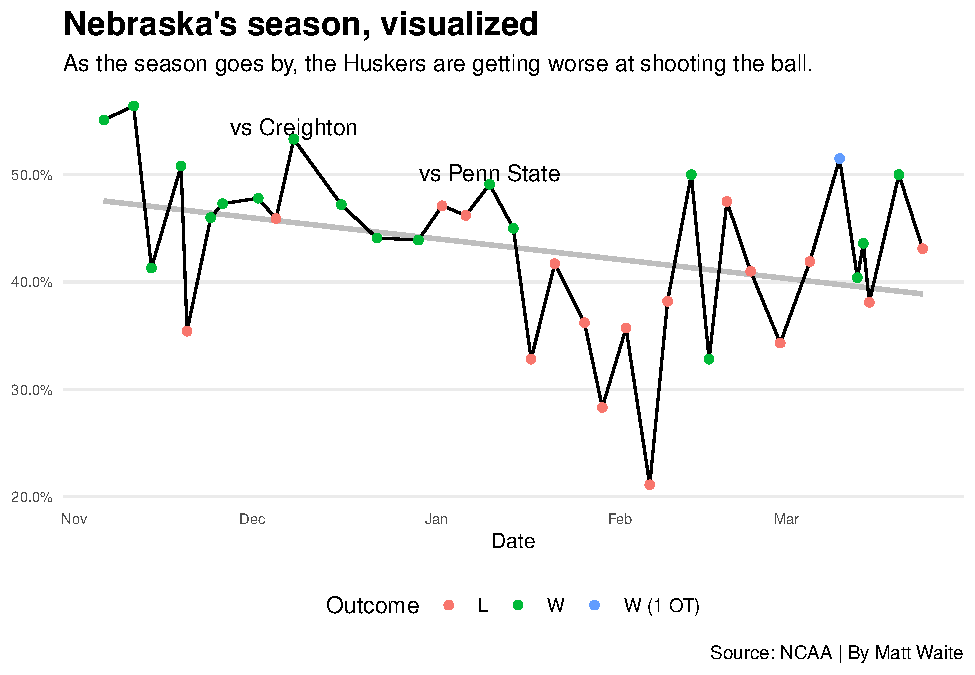
\includegraphics{SportsData_files/figure-latex/unnamed-chunk-54-1.pdf}
Oy. There it is. There's our season.

So I can tell you now, using wide data, that Nebraska's shooting
performance over the last ten games is down 12 percent from the first 10
games. And using long data, I can show you the story of the season, but
without any specific stats to back it up.

\chapter{Simulations}\label{simulations}

Two seasons ago, James Palmer Jr. shot 139 three point attempts and made
43 of them for a .309 shooting percentage last year. A few weeks into
last season, he was 7 for 39 -- a paltry .179. Is something wrong or is
this just bad luck? Let's simulate 39 attempts 1000 times with his
season long shooting percentage and see if this could just be random
chance or something else.

We do this using a base R function called \texttt{rbinom} or binomial
distribution -- another name for a normal distribution. So what that
means is there's a normally distrubuted chance that James Palmer Jr. is
going to shoot above and below his career three point shooting
percentage. If we randomly assign values in that distribution 1000
times, how many times will it come up 7, like this example?

\begin{Shaded}
\begin{Highlighting}[]
\KeywordTok{set.seed}\NormalTok{(}\DecValTok{1234}\NormalTok{)}

\NormalTok{simulations <-}\StringTok{ }\KeywordTok{rbinom}\NormalTok{(}\DataTypeTok{n =} \DecValTok{1000}\NormalTok{, }\DataTypeTok{size =} \DecValTok{39}\NormalTok{, }\DataTypeTok{prob =}\NormalTok{ .}\DecValTok{309}\NormalTok{)}

\KeywordTok{hist}\NormalTok{(simulations)}
\end{Highlighting}
\end{Shaded}

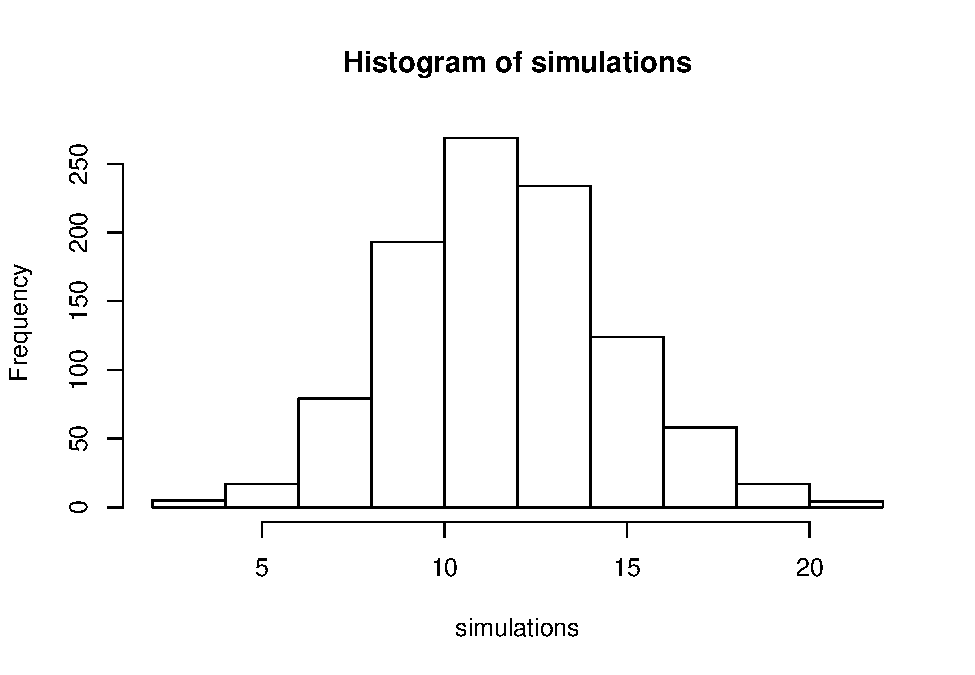
\includegraphics{SportsData_files/figure-latex/unnamed-chunk-55-1.pdf}

\begin{Shaded}
\begin{Highlighting}[]
\KeywordTok{table}\NormalTok{(simulations)}
\end{Highlighting}
\end{Shaded}

\begin{verbatim}
## simulations
##   3   4   5   6   7   8   9  10  11  12  13  14  15  16  17  18  19  20 
##   1   4   5  12  35  44  76 117 134 135 135  99  71  53  37  21  15   2 
##  21  22 
##   3   1
\end{verbatim}

So what we see is given his season long shooting percentage, it's not
out of the realm of randomness that with just 39 attempts for Palmer,
he's only hit only 7. In 1000 simulations, it comes up 35 times. Is he
below where he should be? Yes. Will he likely improve and soon? Yes.

\section{Cold streaks}\label{cold-streaks}

During the Western Illinois game, the team, shooting .329 on the season
from behind the arc, went 0-15 in the second half. How strange is that?

\begin{Shaded}
\begin{Highlighting}[]
\KeywordTok{set.seed}\NormalTok{(}\DecValTok{1234}\NormalTok{)}

\NormalTok{simulations <-}\StringTok{ }\KeywordTok{rbinom}\NormalTok{(}\DataTypeTok{n =} \DecValTok{1000}\NormalTok{, }\DataTypeTok{size =} \DecValTok{15}\NormalTok{, }\DataTypeTok{prob =}\NormalTok{ .}\DecValTok{329}\NormalTok{)}

\KeywordTok{hist}\NormalTok{(simulations)}
\end{Highlighting}
\end{Shaded}

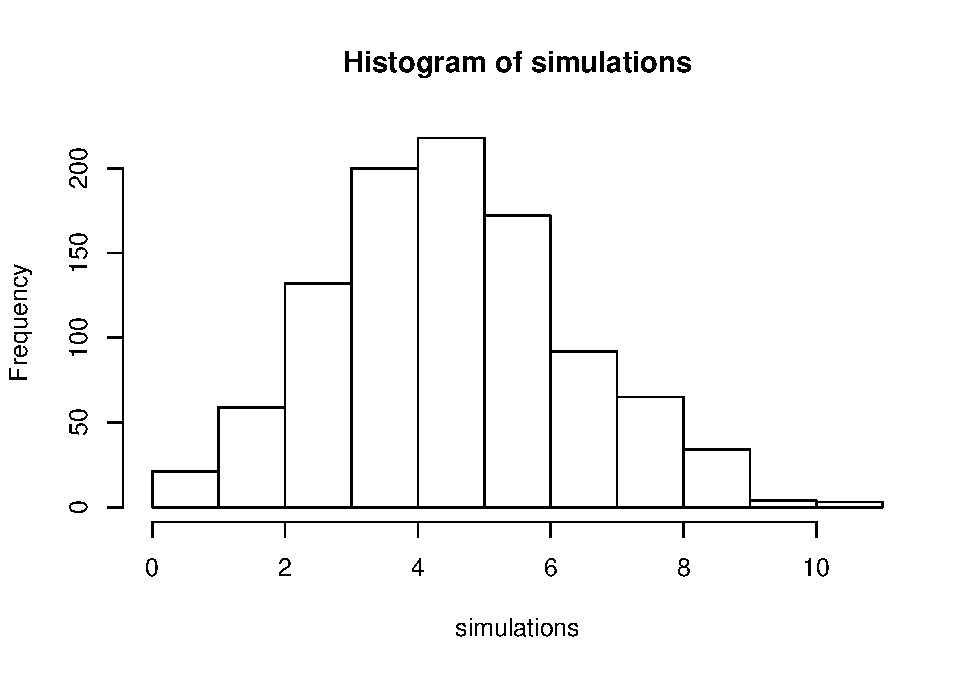
\includegraphics{SportsData_files/figure-latex/unnamed-chunk-56-1.pdf}

\begin{Shaded}
\begin{Highlighting}[]
\KeywordTok{table}\NormalTok{(simulations)}
\end{Highlighting}
\end{Shaded}

\begin{verbatim}
## simulations
##   0   1   2   3   4   5   6   7   8   9  10  11 
##   5  16  59 132 200 218 172  92  65  34   4   3
\end{verbatim}

Short answer: Really weird. If you simulate 15 threes 1000 times,
sometimes you'll see them miss all of them, but only a few times -- five
times, in this case. Most of the time, the team won't go 0-15 even once.
So going ice cold is not totally out of the realm of random chance, but
it's highly unlikely.

\chapter{Correlations and regression}\label{correlations-and-regression}

Throughout sports, you will find no shortage of opinions. From people
yelling at their TV screens to an entire industry of people paid to have
opinions, there are no shortage of reasons why this team sucks and that
player is great. They may have their reasons, but a better question is,
does that reason really matter?

Can we put some numbers behind that? Can we prove it or not?

This is what we're going to start to answer. And we'll do it with
correlations and regressions.

First, we need libraries and
\href{https://unl.box.com/s/zlxoptqixkt98gubk3i6316qun99l49r}{data}.

\begin{Shaded}
\begin{Highlighting}[]
\KeywordTok{library}\NormalTok{(tidyverse)}
\end{Highlighting}
\end{Shaded}

\begin{Shaded}
\begin{Highlighting}[]
\NormalTok{correlations <-}\StringTok{ }\KeywordTok{read_csv}\NormalTok{(}\StringTok{"data/correlations.csv"}\NormalTok{)}
\end{Highlighting}
\end{Shaded}

\begin{verbatim}
## Parsed with column specification:
## cols(
##   Name = col_character(),
##   OffPoints = col_double(),
##   OffPointsG = col_double(),
##   DefPoints = col_double(),
##   DefPointsG = col_double(),
##   Pen. = col_double(),
##   Yards = col_double(),
##   `Pen./G` = col_double(),
##   OffConversions = col_double(),
##   OffConversionPct = col_double(),
##   DefConversions = col_double(),
##   DefConversionPct = col_double()
## )
\end{verbatim}

To do this, we need all FBS college football teams and their season
stats from last year. How much, over the course of a season, does a
thing matter? That's the question you're going to answer.

In our case, we want to know how much does a team's accumulated
penalties influence the number of points they score in a season? How
much difference can we explain in points with penalties?

We're going to use two different methods here and they're closely
related. Correlations -- specifically the Pearson Correlation
Coefficient -- is a measure of how related two numbers are in a linear
fashion. In other words -- if our X value goes up one, what happens to
Y? If it also goes up 1, that's a perfect correlation. X goes up 1, Y
goes up 1. Every time. Correlation coefficients are a number between 0
and 1, with zero being no correlation and 1 being perfect correlation
\textbf{if our data is linear}. We'll soon go over scatterplots to
visually determine if our data is linear, but for now, we have a
hypothesis: More penalties are bad. Penalties hurt. So if a team gets
lots of them, they should have worse outcomes than teams that get few of
them. That is an argument for a linear relationship between them.

But is there one?

We're going create a new dataframe called newcorrelations that takes our
data that we imported and adds a column called \texttt{differential}
because we don't have separate offense and defense penalties, and then
we'll use correlations to see how related those two things are.

\begin{Shaded}
\begin{Highlighting}[]
\NormalTok{newcorrelations <-}\StringTok{ }\NormalTok{correlations }\OperatorTok\StringTok{ }
\StringTok{  }\KeywordTok{mutate}\NormalTok{(}\DataTypeTok{differential =}\NormalTok{ OffPoints }\OperatorTok{-}\StringTok{ }\NormalTok{DefPoints)}
\end{Highlighting}
\end{Shaded}

In R, there is a \texttt{cor} function, and beacuse it's base R, we have
to use a different method of referencing fields that we've not used to
this point. It involves the name of the data frame plus a \texttt{\$}
then the name of the field. So we want to see if \texttt{differential}
is correlated with \texttt{Yards}, which is the yards of penalties a
team gets in a game. We do that by referenceing
\texttt{newcorrelation\$differential} and
\texttt{newcorrelation\$Yards}. The number we get back is the
correlation coefficient.

\begin{Shaded}
\begin{Highlighting}[]
\KeywordTok{cor}\NormalTok{(newcorrelations}\OperatorTok{$}\NormalTok{differential, newcorrelations}\OperatorTok{$}\NormalTok{Yards, }\DataTypeTok{method=}\StringTok{"pearson"}\NormalTok{)}
\end{Highlighting}
\end{Shaded}

\begin{verbatim}
## [1] 0.2008676
\end{verbatim}

So on a scale of 0 to 1, penalty yards and wether or not the team scores
more points than it give up are at .2. You could say they're 20 percent
related. Another way to say it? They're 80 percent not related.

What about the number of penalties instead of the yards?

\begin{Shaded}
\begin{Highlighting}[]
\KeywordTok{cor}\NormalTok{(newcorrelations}\OperatorTok{$}\NormalTok{differential, newcorrelations}\OperatorTok{$}\StringTok{`}\DataTypeTok{Pen.}\StringTok{`}\NormalTok{, }\DataTypeTok{method=}\StringTok{"pearson"}\NormalTok{)}
\end{Highlighting}
\end{Shaded}

\begin{verbatim}
## [1] 0.1534557
\end{verbatim}

Even less related. What about looking at the average? Penalty yards per
game?

\begin{Shaded}
\begin{Highlighting}[]
\KeywordTok{cor}\NormalTok{(newcorrelations}\OperatorTok{$}\NormalTok{differential, newcorrelations}\OperatorTok{$}\StringTok{`}\DataTypeTok{Pen./G}\StringTok{`}\NormalTok{, }\DataTypeTok{method=}\StringTok{"pearson"}\NormalTok{)}
\end{Highlighting}
\end{Shaded}

\begin{verbatim}
## [1] -0.03305037
\end{verbatim}

Not only is it less related, but the relationship is inverted.

So wait, what does that mean?

It means that the number of penalty yards and penalties is actually
positively related to differential. Put another way, teams that have
more penalties and penalty yards tend to have better outcomes. The
average is barely -- 3 percent -- negatively correlated, meaning that
teams with higher averages score fewer points.

What? That makes no sense. How can that be?

Enter regression. Regression is how we try to fit our data into a line
that explains the relationship the best. Regressions will help us
predict things as well -- if we have a team that has so many penalties,
what kind of point differential could we expect, given every FBS team?
So regressions are about prediction, correlations are about description.
Correlations describe a relationship. Regressions help us predict what
that relationship means.

Another thing regressions do is give us some other tools to evaluate if
the relationship is real or not.

Here's an example of using linear modeling to look at yards. Think of
the \texttt{\textasciitilde{}} character as saying ``is predicted by''.
The output looks like a lot, but what we need is a small part of it.

\begin{Shaded}
\begin{Highlighting}[]
\NormalTok{fit <-}\StringTok{ }\KeywordTok{lm}\NormalTok{(differential }\OperatorTok{~}\StringTok{ }\NormalTok{Yards, }\DataTypeTok{data =}\NormalTok{ newcorrelations)}
\KeywordTok{summary}\NormalTok{(fit)}
\end{Highlighting}
\end{Shaded}

\begin{verbatim}
## 
## Call:
## lm(formula = differential ~ Yards, data = newcorrelations)
## 
## Residuals:
##     Min      1Q  Median      3Q     Max 
## -351.02  -93.49    2.67  107.88  444.42 
## 
## Coefficients:
##               Estimate Std. Error t value Pr(>|t|)  
## (Intercept) -108.73848   59.70868  -1.821   0.0709 .
## Yards          0.19484    0.08399   2.320   0.0219 *
## ---
## Signif. codes:  0 '***' 0.001 '**' 0.01 '*' 0.05 '.' 0.1 ' ' 1
## 
## Residual standard error: 140 on 128 degrees of freedom
## Multiple R-squared:  0.04035,    Adjusted R-squared:  0.03285 
## F-statistic: 5.382 on 1 and 128 DF,  p-value: 0.02193
\end{verbatim}

There's three things we need here:

\begin{enumerate}
\def\labelenumi{\arabic{enumi}.}
\tightlist
\item
  First we want to look at the p-value. It's at the bottom right corner
  of the output. In the case of Yards, the p-value is .02193. The
  threshold we're looking for here is .05. If it's less than .05, then
  the relationship is considered to be \emph{statistically significant}.
  Significance here does not mean it's a big deal. It means it's not
  random. That's it. Just that. Not random. So in our case, the
  relationship between penalty yards and a team's aggregate point
  differential are not random. It's a real relationship.
\item
  Second, we look at the Adjusted R-squared value. It's right above the
  p-value. Adjusted R-squared is a measure of how much of the difference
  between teams aggregate point values can be explained by penalty
  yards. Our correlation coefficient said they're 20 percent related to
  each other, but penalty yard's ability to explain the difference
  between teams? About 3.3 percent. That's \ldots{} not much. It's
  really nothing.
\item
  The third thing we can look at, and we only bother if the first two
  are meaningful, is the coefficients. In the middle, you can see the
  (Intercept) is -108.73848 and the Yards coefficient is .19484.
  Remember high school algebra? Remember learning the equation of a
  line? Remember swearing that learning \texttt{y=mx+b} is stupid
  because you'll never need it again? Surprise. It's useful again. In
  this case, we could try to predict a team's aggregate score in a
  season -- will they score more than they give up -- by using
  \texttt{y=mx+b}. In this case, y is the aggregate score, m is .19484
  and b is -108.73848. So we would multiply a teams total penalty yards
  by .19484 and then subtract 108.73848 from it. The result would tell
  you what the total aggregate score in the season would be. Chance that
  your even close with this? About 3 percent.
\end{enumerate}

You can see the problem in a graph. On the X axis is penalty yards, on
the y is aggregate score. If these elements had a strong relationship,
we'd see a clear pattern moving from right to left, sloping down. Onn
the left would be the teams with lots of penalty yards and a negative
point differential. On right would be teams with low penalty yards and
high point differentials. Do you see that below?

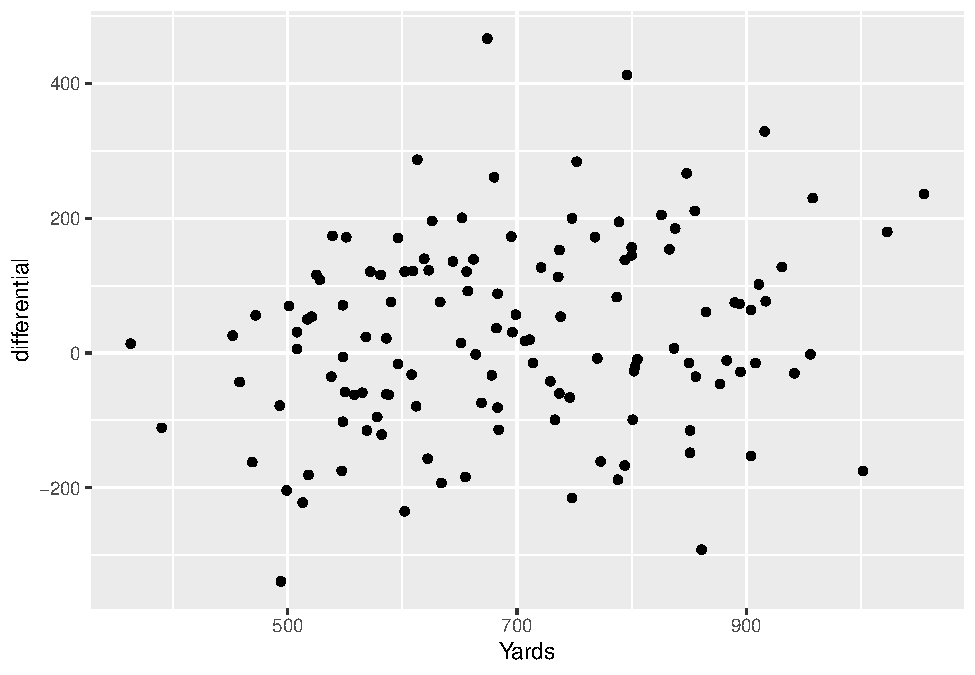
\includegraphics{SportsData_files/figure-latex/unnamed-chunk-64-1.pdf}

\begin{quote}
\textbf{Your turn}: Try it with the other penalty measures. Total
penalties and penalty yards per game. Does anything change? Do either of
these meet the .05 threshold for randomness? Are either of these any
more predictive?
\end{quote}

\section{A more predictive example}\label{a-more-predictive-example}

So we've firmly established that penalties aren't predictive. But what
is? One measure I've found to be highly predictive of a team's success
is how well do they do on third down. It's simple really: Succeed on
third down, you get to stay on offense. Fail on third down, you are
punting (most likely) or settling for a field goal. Either way, you're
scoring less than you would by scoring touchdowns. How related are
points per game and third down conversion percentage?

\begin{Shaded}
\begin{Highlighting}[]
\KeywordTok{cor}\NormalTok{(newcorrelations}\OperatorTok{$}\NormalTok{OffPointsG, newcorrelations}\OperatorTok{$}\NormalTok{OffConversionPct, }\DataTypeTok{method=}\StringTok{"pearson"}\NormalTok{)}
\end{Highlighting}
\end{Shaded}

\begin{verbatim}
## [1] 0.6658862
\end{verbatim}

Answer: 67 percent. More than three times more related than penalty
yards. But how meaningful is that relationship and how predictive is it?

\begin{Shaded}
\begin{Highlighting}[]
\NormalTok{third <-}\StringTok{ }\KeywordTok{lm}\NormalTok{(OffPointsG }\OperatorTok{~}\StringTok{ }\NormalTok{OffConversionPct, }\DataTypeTok{data =}\NormalTok{ newcorrelations)}
\KeywordTok{summary}\NormalTok{(third)}
\end{Highlighting}
\end{Shaded}

\begin{verbatim}
## 
## Call:
## lm(formula = OffPointsG ~ OffConversionPct, data = newcorrelations)
## 
## Residuals:
##      Min       1Q   Median       3Q      Max 
## -11.3861  -3.5411  -0.5885   2.9011  13.5188 
## 
## Coefficients:
##                  Estimate Std. Error t value Pr(>|t|)    
## (Intercept)      -4.74024    3.41041   -1.39    0.167    
## OffConversionPct  0.85625    0.08479   10.10   <2e-16 ***
## ---
## Signif. codes:  0 '***' 0.001 '**' 0.01 '*' 0.05 '.' 0.1 ' ' 1
## 
## Residual standard error: 5.111 on 128 degrees of freedom
## Multiple R-squared:  0.4434, Adjusted R-squared:  0.4391 
## F-statistic:   102 on 1 and 128 DF,  p-value: < 2.2e-16
\end{verbatim}

First we check p-value. See that e-16? That means scientific notation.
That means our number is 2.2 times 10 to the -16 power. So
-.000000000000000022. That's sixteen zeros between the decimal and 22.
Is that less than .05? Uh, yeah. So this is really, really, really not
random. But anyone who has watched a game of football knows this is
true. It makes intuitive sense.

Second, Adjusted R-squared: .4391. So we can predict 44 percent of the
difference in the total offensive points per game a team scores by
simply looking at their third down conversion percentage. Third, the
coefficients: In this case, our \texttt{y=mx+b} formula looks like
\texttt{y\ =\ .85625x-4.74024}. So if we were applying this, let's look
at Nebraska's 31-28 loss to Iowa on Black Friday in 2018. Nebraska was
6-15 on third down in that game, or 40 percent (Iowa was 7 of 13 or 54
percent). Given those numbers, our formula predicts Nebraska should have
scored how many points?

\begin{Shaded}
\begin{Highlighting}[]
\NormalTok{(}\FloatTok{0.85625} \OperatorTok{*}\StringTok{ }\DecValTok{40}\NormalTok{) }\OperatorTok{-}\StringTok{ }\FloatTok{4.74024} 
\end{Highlighting}
\end{Shaded}

\begin{verbatim}
## [1] 29.50976
\end{verbatim}

That's really close to the 28 they did score. And Iowa?

\begin{Shaded}
\begin{Highlighting}[]
\NormalTok{(}\FloatTok{0.85625} \OperatorTok{*}\StringTok{ }\DecValTok{54}\NormalTok{) }\OperatorTok{-}\StringTok{ }\FloatTok{4.74024} 
\end{Highlighting}
\end{Shaded}

\begin{verbatim}
## [1] 41.49726
\end{verbatim}

By our model, Iowa should have scored 10 more points than they did. But
they didn't. Why, besides Iowa is terrible and deserves punishment from
the football gods for being Iowa? Remember our model can only explain 44
percent of the points. There's more to football than one metric.

\chapter{Multiple regression}\label{multiple-regression}

Last chapter, we looked at correlations and linear regression to predict
how one element of a game would predict the score. But we know that a
single variable, in all but the rarest instances, are not going to be
that predictive. We need more than one. Enter multiple regression.
Multiple regression lets us add -- wait for it -- mulitiple predictors
to our equation to help us get a better

That presents it's own problems. So let's get our libraries and our
data, this time of
\href{https://unl.box.com/s/u9407jj007fxtnu1vbkybdawaqg6j3fw}{every
college basketball game since the 2014-15 season} loaded up.

\begin{Shaded}
\begin{Highlighting}[]
\KeywordTok{library}\NormalTok{(tidyverse)}
\end{Highlighting}
\end{Shaded}

\begin{Shaded}
\begin{Highlighting}[]
\NormalTok{logs <-}\StringTok{ }\KeywordTok{read_csv}\NormalTok{(}\StringTok{"data/logs1519.csv"}\NormalTok{)}
\end{Highlighting}
\end{Shaded}

\begin{verbatim}
## Warning: Missing column names filled in: 'X1' [1]
\end{verbatim}

\begin{verbatim}
## Parsed with column specification:
## cols(
##   .default = col_double(),
##   Date = col_date(format = ""),
##   HomeAway = col_character(),
##   Opponent = col_character(),
##   W_L = col_character(),
##   Blank = col_logical(),
##   Team = col_character(),
##   Conference = col_character(),
##   season = col_character()
## )
\end{verbatim}

\begin{verbatim}
## See spec(...) for full column specifications.
\end{verbatim}

So one way to show how successful a basketball team was for a game is to
show the differential between the team's score and the opponnent's
score. Score a lot more than the opponent = good, score a lot less than
the opponent = bad. And, relatively speaking, the more the better. So
let's create that differential.

\begin{Shaded}
\begin{Highlighting}[]
\NormalTok{logs <-}\StringTok{ }\NormalTok{logs }\OperatorTok\StringTok{ }\KeywordTok{mutate}\NormalTok{(}\DataTypeTok{Differential =}\NormalTok{ TeamScore }\OperatorTok{-}\StringTok{ }\NormalTok{OpponentScore)}
\end{Highlighting}
\end{Shaded}

The linear model code we used before is pretty straight forward. Its
\texttt{field} is predicted by \texttt{field}. Here's a simple linear
model that looks at predicting a team's point differential by looking at
their offensive shooting percentage.

\begin{Shaded}
\begin{Highlighting}[]
\NormalTok{shooting <-}\StringTok{ }\KeywordTok{lm}\NormalTok{(TeamFGPCT }\OperatorTok{~}\StringTok{ }\NormalTok{Differential, }\DataTypeTok{data=}\NormalTok{logs)}
\KeywordTok{summary}\NormalTok{(shooting)}
\end{Highlighting}
\end{Shaded}

\begin{verbatim}
## 
## Call:
## lm(formula = TeamFGPCT ~ Differential, data = logs)
## 
## Residuals:
##       Min        1Q    Median        3Q       Max 
## -0.260485 -0.040230 -0.001096  0.039038  0.267457 
## 
## Coefficients:
##               Estimate Std. Error t value Pr(>|t|)    
## (Intercept)  4.399e-01  2.487e-04  1768.4   <2e-16 ***
## Differential 2.776e-03  1.519e-05   182.8   <2e-16 ***
## ---
## Signif. codes:  0 '***' 0.001 '**' 0.01 '*' 0.05 '.' 0.1 ' ' 1
## 
## Residual standard error: 0.05949 on 57514 degrees of freedom
##   (4 observations deleted due to missingness)
## Multiple R-squared:  0.3675, Adjusted R-squared:  0.3674 
## F-statistic: 3.341e+04 on 1 and 57514 DF,  p-value: < 2.2e-16
\end{verbatim}

Remember: There's a lot here, but only some of it we care about. What is
the Adjusted R-squared value? What's the p-value and is it less than
.05? In this case, we can predict 37 percent of the difference in
differential with how well a team shoots the ball.

To add more predictors to this mix, we merely add them. But it's not
that simple, as you'll see in a moment. So first, let's look at adding
how well the other team shot to our prediction model:

\begin{Shaded}
\begin{Highlighting}[]
\NormalTok{model1 <-}\StringTok{ }\KeywordTok{lm}\NormalTok{(Differential }\OperatorTok{~}\StringTok{ }\NormalTok{TeamFGPCT }\OperatorTok{+}\StringTok{ }\NormalTok{OpponentFGPCT, }\DataTypeTok{data=}\NormalTok{logs)}
\KeywordTok{summary}\NormalTok{(model1)}
\end{Highlighting}
\end{Shaded}

\begin{verbatim}
## 
## Call:
## lm(formula = Differential ~ TeamFGPCT + OpponentFGPCT, data = logs)
## 
## Residuals:
##     Min      1Q  Median      3Q     Max 
## -49.591  -6.185  -0.198   5.938  68.344 
## 
## Coefficients:
##                Estimate Std. Error  t value Pr(>|t|)    
## (Intercept)      1.1195     0.3483    3.214  0.00131 ** 
## TeamFGPCT      118.5211     0.5279  224.518  < 2e-16 ***
## OpponentFGPCT -119.9369     0.5252 -228.372  < 2e-16 ***
## ---
## Signif. codes:  0 '***' 0.001 '**' 0.01 '*' 0.05 '.' 0.1 ' ' 1
## 
## Residual standard error: 9.407 on 57513 degrees of freedom
##   (4 observations deleted due to missingness)
## Multiple R-squared:  0.6683, Adjusted R-squared:  0.6683 
## F-statistic: 5.793e+04 on 2 and 57513 DF,  p-value: < 2.2e-16
\end{verbatim}

First things first: What is the adjusted R-squared?

Second: what is the p-value and is it less than .05?

Third: Compare the residual standard error. We went from .05949 to 9.4.
The meaning of this is both really opaque and also simple -- we added a
lot of error to our model by adding more measures -- 158 times more.
Residual standard error is the total distance between what our model
would predict and what we actually have in the data. So lots of residual
error means the distance between reality and our model is wider. So the
width of our predictive range in this example grew pretty dramatically,
but so did the amount of the difference we could predict. It's a trade
off.

One of the more difficult things to understand about multiple regression
is the issue of multicollinearity. What that means is that there is
significant correlation overlap between two variables -- the two are
related to each other as well as to the target output -- and all you are
doing by adding both of them is adding error with no real value to the
R-squared. In pure statistics, we don't want any multicollinearity at
all. Violating that assumption limits the applicability of what you are
doing. So if we have some multicollinearity, it limits our scope of
application to college basketball. We can't say this will work for every
basketball league and level everywhere. What we need to do is see how
correlated each value is to each other and throw out ones that are
highly co-correlated.

So to find those, we have to create a correlation matrix that shows us
how each value is correlated to our outcome variable, but also with each
other. We can do that in the \texttt{Hmisc} library. We install that in
the console with \texttt{install.packages("Hmisc")}

\begin{Shaded}
\begin{Highlighting}[]
\KeywordTok{library}\NormalTok{(Hmisc)}
\end{Highlighting}
\end{Shaded}

We can pass in every numeric value to the Hmisc library and get a
correlation matrix out of it, but since we have a large number of values
-- and many of them character values -- we should strip that down and
reorder them. So that's what I'm doing here. I'm saying give me
differential first, and then columns 9-24, and then 26-41. Why the skip?
There's a blank column in the middle of the data -- a remnant of the
scraper I used.

\begin{Shaded}
\begin{Highlighting}[]
\NormalTok{simplelogs <-}\StringTok{ }\NormalTok{logs }\OperatorTok\StringTok{ }\KeywordTok{select}\NormalTok{(Differential, }\DecValTok{9}\OperatorTok{:}\DecValTok{24}\NormalTok{, }\DecValTok{26}\OperatorTok{:}\DecValTok{41}\NormalTok{)}
\end{Highlighting}
\end{Shaded}

Before we proceed, what we're looking to do is follow the Differential
column down, looking for correlation values near 1 or -1. Correlations
go from -1, meaning perfect negative correlation, to 0, meaning no
correlation, to 1, meaning perfect positive correlation. So we're
looking for numbers near 1 or -1 for their predictive value. BUT: We
then need to see if that value is also highly correlated with something
else. If it is, we have a decision to make.

We get our correlation matrix like this:

\begin{Shaded}
\begin{Highlighting}[]
\NormalTok{cormatrix <-}\StringTok{ }\KeywordTok{rcorr}\NormalTok{(}\KeywordTok{as.matrix}\NormalTok{(simplelogs))}

\NormalTok{cormatrix}\OperatorTok{$}\NormalTok{r}
\end{Highlighting}
\end{Shaded}

\begin{verbatim}
##                       Differential       TeamFG      TeamFGA    TeamFGPCT
## Differential           1.000000000  0.584766682  0.107389235  0.606178206
## TeamFG                 0.584766682  1.000000000  0.563220974  0.751715176
## TeamFGA                0.107389235  0.563220974  1.000000000 -0.109620267
## TeamFGPCT              0.606178206  0.751715176 -0.109620267  1.000000000
## Team3P                 0.318300418  0.408787900  0.213352219  0.322872202
## Team3PA                0.056680627  0.179527313  0.426011924 -0.119421368
## Team3PPCT              0.367934059  0.380235821 -0.101463821  0.545986963
## TeamFT                 0.238182740 -0.022308582 -0.137853824  0.084649669
## TeamFTA                0.206075949 -0.027927391 -0.129851346  0.070632302
## TeamFTPCT              0.138833800  0.016247282 -0.044394472  0.056887587
## TeamOffRebounds        0.136095147  0.161626257  0.545231683 -0.234244567
## TeamTotalRebounds      0.470722398  0.328460524  0.470719037  0.018581908
## TeamAssists            0.540398009  0.664057724  0.284659104  0.566152928
## TeamSteals             0.277670288  0.210221346  0.208743124  0.080191710
## TeamBlocks             0.257608076  0.140856644  0.074555286  0.107327505
## TeamTurnovers         -0.180578328 -0.143210529 -0.223971265  0.001901048
## TeamPersonalFouls     -0.194427271 -0.014722266  0.107325560 -0.094653222
## OpponentFG            -0.538515115  0.144061400  0.256737262 -0.020183466
## OpponentFGA            0.001768386  0.302143806  0.301593528  0.126415534
## OpponentFGPCT         -0.614427717 -0.058571888  0.068034775 -0.114791403
## Opponent3P            -0.283754971  0.131517138  0.135290090  0.053105214
## Opponent3PA            0.013910296  0.191131927  0.138445785  0.118723805
## Opponent3PPCT         -0.382427841  0.008026622  0.057261756 -0.031370545
## OpponentFT            -0.269300868  0.019511923  0.157025930 -0.091558712
## OpponentFTA           -0.226064714  0.012937366  0.159529646 -0.101685664
## OpponentFTPCT         -0.175223632  0.007923359  0.023732217 -0.006190565
## OpponentOffRebounds   -0.089347536 -0.036316958  0.002848058 -0.042399744
## OpponentTotalRebounds -0.420010794 -0.225202127  0.316139528 -0.512983306
## OpponentAssists       -0.491676030  0.004558539  0.149320067 -0.106252682
## OpponentSteals        -0.187754380 -0.102436608 -0.131734964 -0.021724636
## OpponentBlocks        -0.262252627 -0.160469663  0.218483865 -0.356255034
## OpponentTurnovers      0.274326954  0.155293275  0.198127970  0.024254833
## OpponentPersonalFouls  0.169025733 -0.023116620 -0.107189301  0.060150658
##                             Team3P     Team3PA     Team3PPCT       TeamFT
## Differential           0.318300418  0.05668063  0.3679340589  0.238182740
## TeamFG                 0.408787900  0.17952731  0.3802358207 -0.022308582
## TeamFGA                0.213352219  0.42601192 -0.1014638212 -0.137853824
## TeamFGPCT              0.322872202 -0.11942137  0.5459869634  0.084649669
## Team3P                 1.000000000  0.70114773  0.7073663404 -0.106344056
## Team3PA                0.701147726  1.00000000  0.0407645751 -0.160515313
## Team3PPCT              0.707366340  0.04076458  1.0000000000  0.005129556
## TeamFT                -0.106344056 -0.16051531  0.0051295561  1.000000000
## TeamFTA               -0.137499074 -0.18150913 -0.0180696209  0.927525817
## TeamFTPCT              0.048777304  0.01119250  0.0553684315  0.387017653
## TeamOffRebounds       -0.062026229  0.12484929 -0.1968568361  0.087168289
## TeamTotalRebounds      0.038344971  0.12095682 -0.0628970009  0.190691619
## TeamAssists            0.519530086  0.28786139  0.4326950943 -0.016343370
## TeamSteals             0.016545254  0.04598400 -0.0246657289  0.088535320
## TeamBlocks             0.004747719 -0.02895321  0.0294277389  0.092392379
## TeamTurnovers         -0.088374940 -0.10883919 -0.0209433827  0.051609207
## TeamPersonalFouls     -0.024028303  0.02499520 -0.0498165852  0.217846416
## OpponentFG             0.123800594  0.15638030  0.0296913406  0.057853338
## OpponentFGA            0.148931744  0.13062824  0.0812237901  0.193116094
## OpponentFGPCT          0.029908235  0.08057726 -0.0264843759 -0.075399282
## Opponent3P             0.079455775  0.07482590  0.0402012413  0.024228311
## Opponent3PA            0.085704376  0.05927299  0.0601150176  0.079894905
## Opponent3PPCT          0.029666235  0.04634676  0.0005076038 -0.035478488
## OpponentFT             0.009796521  0.06316300 -0.0390873639  0.161311559
## OpponentFTA           -0.002503282  0.05474884 -0.0480732723  0.183801456
## OpponentFTPCT          0.022780414  0.02587876  0.0086512859 -0.015688533
## OpponentOffRebounds   -0.007870292 -0.01895081  0.0086776821  0.064938518
## OpponentTotalRebounds -0.062384273  0.20289676 -0.2638845414 -0.064969878
## OpponentAssists        0.029413582  0.08254506 -0.0320289494 -0.057730062
## OpponentSteals        -0.053878305 -0.05298037 -0.0251316716 -0.001883349
## OpponentBlocks        -0.111782062 -0.05804217 -0.0965607977 -0.065055523
## OpponentTurnovers      0.009284106  0.06383515 -0.0488449748  0.136922084
## OpponentPersonalFouls -0.127197007 -0.15536393 -0.0268876881  0.793539202
##                            TeamFTA    TeamFTPCT TeamOffRebounds
## Differential           0.206075949  0.138833800    0.1360951470
## TeamFG                -0.027927391  0.016247282    0.1616262575
## TeamFGA               -0.129851346 -0.044394472    0.5452316831
## TeamFGPCT              0.070632302  0.056887587   -0.2342445674
## Team3P                -0.137499074  0.048777304   -0.0620262290
## Team3PA               -0.181509133  0.011192503    0.1248492948
## Team3PPCT             -0.018069621  0.055368431   -0.1968568361
## TeamFT                 0.927525817  0.387017653    0.0871682888
## TeamFTA                1.000000000  0.053233778    0.1415933172
## TeamFTPCT              0.053233778  1.000000000   -0.0948040467
## TeamOffRebounds        0.141593317 -0.094804047    1.0000000000
## TeamTotalRebounds      0.231278690 -0.037356471    0.6373027887
## TeamAssists           -0.028289202  0.025948025    0.0509277222
## TeamSteals             0.111199125 -0.025969502    0.1195581042
## TeamBlocks             0.104112579 -0.001425412    0.1060163877
## TeamTurnovers          0.072070652 -0.034614485    0.0371728710
## TeamPersonalFouls      0.250787085 -0.025827923    0.0542337992
## OpponentFG             0.043602296  0.036986356   -0.0464694335
## OpponentFGA            0.193466766  0.040334507    0.0242353640
## OpponentFGPCT         -0.091897172  0.012864509   -0.0688833747
## Opponent3P             0.009600704  0.031763685   -0.0063710321
## Opponent3PA            0.071193179  0.032554796    0.0003753868
## Opponent3PPCT         -0.047136861  0.013996880   -0.0056578317
## OpponentFT             0.180010001 -0.009352580    0.0434399899
## OpponentFTA            0.213209437 -0.025707797    0.0584669041
## OpponentFTPCT         -0.032862991  0.028078614   -0.0319032781
## OpponentOffRebounds    0.077003661 -0.016936223   -0.0143325753
## OpponentTotalRebounds  0.004736343 -0.177541483   -0.0603891339
## OpponentAssists       -0.063875391 -0.007401206   -0.0386521955
## OpponentSteals         0.006758108 -0.022033431    0.0326977763
## OpponentBlocks        -0.053973588 -0.041175463    0.1571812909
## OpponentTurnovers      0.169704736 -0.035463921    0.1154717115
## OpponentPersonalFouls  0.866395092  0.018757079    0.1240631120
##                       TeamTotalRebounds   TeamAssists   TeamSteals
## Differential                0.470722398  0.5403980088  0.277670288
## TeamFG                      0.328460524  0.6640577242  0.210221346
## TeamFGA                     0.470719037  0.2846591045  0.208743124
## TeamFGPCT                   0.018581908  0.5661529279  0.080191710
## Team3P                      0.038344971  0.5195300862  0.016545254
## Team3PA                     0.120956819  0.2878613903  0.045984003
## Team3PPCT                  -0.062897001  0.4326950943 -0.024665729
## TeamFT                      0.190691619 -0.0163433697  0.088535320
## TeamFTA                     0.231278690 -0.0282892019  0.111199125
## TeamFTPCT                  -0.037356471  0.0259480253 -0.025969502
## TeamOffRebounds             0.637302789  0.0509277222  0.119558104
## TeamTotalRebounds           1.000000000  0.2321524530  0.027446991
## TeamAssists                 0.232152453  1.0000000000  0.164837110
## TeamSteals                  0.027446991  0.1648371104  1.000000000
## TeamBlocks                  0.265518873  0.1447645615  0.065539758
## TeamTurnovers               0.109155292 -0.0789200586  0.078278779
## TeamPersonalFouls          -0.007423332 -0.1050900267  0.005151965
## OpponentFG                 -0.229331788 -0.0022308763 -0.138728115
## OpponentFGA                 0.360268614  0.1863368268 -0.120696505
## OpponentFGPCT              -0.530432484 -0.1397140493 -0.068951590
## Opponent3P                 -0.053371243  0.0354785684 -0.062074442
## Opponent3PA                 0.232049186  0.1116023406 -0.039184667
## Opponent3PPCT              -0.273572339 -0.0502063543 -0.047114732
## OpponentFT                 -0.095266106 -0.0835716395 -0.034152581
## OpponentFTA                -0.022971823 -0.0841605708 -0.022178476
## OpponentFTPCT              -0.194279344 -0.0278263543 -0.041125993
## OpponentOffRebounds        -0.052416263 -0.0333847454  0.016707012
## OpponentTotalRebounds      -0.059965631 -0.2225952122  0.035155522
## OpponentAssists            -0.218597433  0.0006884142 -0.053327136
## OpponentSteals              0.066119486 -0.0288668673  0.055697260
## OpponentBlocks              0.013924890 -0.1657235463 -0.002230784
## OpponentTurnovers          -0.034355689  0.1314533533  0.730885169
## OpponentPersonalFouls       0.189144014 -0.0267820830  0.071442012
##                         TeamBlocks TeamTurnovers TeamPersonalFouls
## Differential           0.257608076  -0.180578328      -0.194427271
## TeamFG                 0.140856644  -0.143210529      -0.014722266
## TeamFGA                0.074555286  -0.223971265       0.107325560
## TeamFGPCT              0.107327505   0.001901048      -0.094653222
## Team3P                 0.004747719  -0.088374940      -0.024028303
## Team3PA               -0.028953212  -0.108839191       0.024995197
## Team3PPCT              0.029427739  -0.020943383      -0.049816585
## TeamFT                 0.092392379   0.051609207       0.217846416
## TeamFTA                0.104112579   0.072070652       0.250787085
## TeamFTPCT             -0.001425412  -0.034614485      -0.025827923
## TeamOffRebounds        0.106016388   0.037172871       0.054233799
## TeamTotalRebounds      0.265518873   0.109155292      -0.007423332
## TeamAssists            0.144764562  -0.078920059      -0.105090027
## TeamSteals             0.065539758   0.078278779       0.005151965
## TeamBlocks             1.000000000   0.032775757      -0.054105029
## TeamTurnovers          0.032775757   1.000000000       0.220285924
## TeamPersonalFouls     -0.054105029   0.220285924       1.000000000
## OpponentFG            -0.143969401   0.081879049      -0.015422966
## OpponentFGA            0.257245080   0.155947902      -0.122639976
## OpponentFGPCT         -0.353110391  -0.023017156       0.078411084
## Opponent3P            -0.103465578  -0.018088322      -0.126817358
## Opponent3PA           -0.042234814   0.041669476      -0.167647391
## Opponent3PPCT         -0.099440199  -0.063187150      -0.015909552
## OpponentFT            -0.070920662   0.123594852       0.793147614
## OpponentFTA           -0.056095076   0.154110278       0.865844664
## OpponentFTPCT         -0.052504157  -0.034267574       0.026877590
## OpponentOffRebounds    0.178200671   0.074131214       0.122282037
## OpponentTotalRebounds  0.037788375  -0.106168146       0.195017438
## OpponentAssists       -0.151146052   0.072644677      -0.022619097
## OpponentSteals         0.028453380   0.709987911       0.064446997
## OpponentBlocks        -0.038978593   0.006463872       0.087211248
## OpponentTurnovers      0.031375703   0.188537020       0.101693555
## OpponentPersonalFouls  0.080582762   0.131539040       0.322258517
##                         OpponentFG  OpponentFGA OpponentFGPCT   Opponent3P
## Differential          -0.538515115  0.001768386  -0.614427717 -0.283754971
## TeamFG                 0.144061400  0.302143806  -0.058571888  0.131517138
## TeamFGA                0.256737262  0.301593528   0.068034775  0.135290090
## TeamFGPCT             -0.020183466  0.126415534  -0.114791403  0.053105214
## Team3P                 0.123800594  0.148931744   0.029908235  0.079455775
## Team3PA                0.156380301  0.130628244   0.080577258  0.074825900
## Team3PPCT              0.029691341  0.081223790  -0.026484376  0.040201241
## TeamFT                 0.057853338  0.193116094  -0.075399282  0.024228311
## TeamFTA                0.043602296  0.193466766  -0.091897172  0.009600704
## TeamFTPCT              0.036986356  0.040334507   0.012864509  0.031763685
## TeamOffRebounds       -0.046469434  0.024235364  -0.068883375 -0.006371032
## TeamTotalRebounds     -0.229331788  0.360268614  -0.530432484 -0.053371243
## TeamAssists           -0.002230876  0.186336827  -0.139714049  0.035478568
## TeamSteals            -0.138728115 -0.120696505  -0.068951590 -0.062074442
## TeamBlocks            -0.143969401  0.257245080  -0.353110391 -0.103465578
## TeamTurnovers          0.081879049  0.155947902  -0.023017156 -0.018088322
## TeamPersonalFouls     -0.015422966 -0.122639976   0.078411084 -0.126817358
## OpponentFG             1.000000000  0.515517123   0.754791141  0.399027442
## OpponentFGA            0.515517123  1.000000000  -0.161220379  0.193563166
## OpponentFGPCT          0.754791141 -0.161220379   1.000000000  0.312295571
## Opponent3P             0.399027442  0.193563166   0.312295571  1.000000000
## Opponent3PA            0.144074778  0.418730422  -0.149367436  0.691451820
## Opponent3PPCT          0.395540055 -0.118020866   0.552279238  0.709404126
## OpponentFT            -0.013421944 -0.156152803   0.106226566 -0.106344743
## OpponentFTA           -0.027151720 -0.151706668   0.086625216 -0.140194309
## OpponentFTPCT          0.037049836 -0.043324702   0.076650746  0.053774302
## OpponentOffRebounds    0.120715447  0.519792207  -0.251623986 -0.085432899
## OpponentTotalRebounds  0.275438081  0.424276325  -0.005789348  0.005903551
## OpponentAssists        0.638304131  0.231851475   0.553535793  0.513869716
## OpponentSteals         0.140823916  0.165329579   0.036468797 -0.011661373
## OpponentBlocks         0.129076992  0.045565883   0.111935521 -0.004746412
## OpponentTurnovers     -0.183558009 -0.215633733  -0.048082678 -0.095218199
## OpponentPersonalFouls  0.015334210  0.136789046  -0.081776664 -0.011247805
##                         Opponent3PA Opponent3PPCT   OpponentFT
## Differential           0.0139102958 -0.3824278411 -0.269300868
## TeamFG                 0.1911319274  0.0080266219  0.019511923
## TeamFGA                0.1384457845  0.0572617563  0.157025930
## TeamFGPCT              0.1187238045 -0.0313705446 -0.091558712
## Team3P                 0.0857043764  0.0296662353  0.009796521
## Team3PA                0.0592729911  0.0463467602  0.063163000
## Team3PPCT              0.0601150176  0.0005076038 -0.039087364
## TeamFT                 0.0798949051 -0.0354784876  0.161311559
## TeamFTA                0.0711931792 -0.0471368607  0.180010001
## TeamFTPCT              0.0325547961  0.0139968801 -0.009352580
## TeamOffRebounds        0.0003753868 -0.0056578317  0.043439990
## TeamTotalRebounds      0.2320491861 -0.2735723395 -0.095266106
## TeamAssists            0.1116023406 -0.0502063543 -0.083571639
## TeamSteals            -0.0391846669 -0.0471147320 -0.034152581
## TeamBlocks            -0.0422348142 -0.0994401990 -0.070920662
## TeamTurnovers          0.0416694763 -0.0631871498  0.123594852
## TeamPersonalFouls     -0.1676473908 -0.0159095518  0.793147614
## OpponentFG             0.1440747785  0.3955400546 -0.013421944
## OpponentFGA            0.4187304220 -0.1180208656 -0.156152803
## OpponentFGPCT         -0.1493674362  0.5522792378  0.106226566
## Opponent3P             0.6914518201  0.7094041257 -0.106344743
## Opponent3PA            1.0000000000  0.0303822862 -0.174340043
## Opponent3PPCT          0.0303822862  1.0000000000  0.016928291
## OpponentFT            -0.1743400433  0.0169282910  1.000000000
## OpponentFTA           -0.1972872368 -0.0080249496  0.928286066
## OpponentFTPCT          0.0101886734  0.0623587723  0.393203255
## OpponentOffRebounds    0.0978389488 -0.2013096986  0.086671729
## OpponentTotalRebounds  0.0810576009 -0.0680836101  0.197591588
## OpponentAssists        0.2641728450  0.4428640799 -0.012378006
## OpponentSteals         0.0214481397 -0.0383569868  0.077614062
## OpponentBlocks        -0.0495426307  0.0354134646  0.101422181
## OpponentTurnovers     -0.0944428800 -0.0421344973  0.015778567
## OpponentPersonalFouls  0.0396475169 -0.0466461289  0.215609923
##                        OpponentFTA OpponentFTPCT OpponentOffRebounds
## Differential          -0.226064714  -0.175223632        -0.089347536
## TeamFG                 0.012937366   0.007923359        -0.036316958
## TeamFGA                0.159529646   0.023732217         0.002848058
## TeamFGPCT             -0.101685664  -0.006190565        -0.042399744
## Team3P                -0.002503282   0.022780414        -0.007870292
## Team3PA                0.054748838   0.025878762        -0.018950808
## Team3PPCT             -0.048073272   0.008651286         0.008677682
## TeamFT                 0.183801456  -0.015688533         0.064938518
## TeamFTA                0.213209437  -0.032862991         0.077003661
## TeamFTPCT             -0.025707797   0.028078614        -0.016936223
## TeamOffRebounds        0.058466904  -0.031903278        -0.014332575
## TeamTotalRebounds     -0.022971823  -0.194279344        -0.052416263
## TeamAssists           -0.084160571  -0.027826354        -0.033384745
## TeamSteals            -0.022178476  -0.041125993         0.016707012
## TeamBlocks            -0.056095076  -0.052504157         0.178200671
## TeamTurnovers          0.154110278  -0.034267574         0.074131214
## TeamPersonalFouls      0.865844664   0.026877590         0.122282037
## OpponentFG            -0.027151720   0.037049836         0.120715447
## OpponentFGA           -0.151706668  -0.043324702         0.519792207
## OpponentFGPCT          0.086625216   0.076650746        -0.251623986
## Opponent3P            -0.140194309   0.053774302        -0.085432899
## Opponent3PA           -0.197287237   0.010188673         0.097838949
## Opponent3PPCT         -0.008024950   0.062358772        -0.201309699
## OpponentFT             0.928286066   0.393203255         0.086671729
## OpponentFTA            1.000000000   0.063446167         0.136423744
## OpponentFTPCT          0.063446167   1.000000000        -0.082982260
## OpponentOffRebounds    0.136423744  -0.082982260         1.000000000
## OpponentTotalRebounds  0.232447345  -0.021281750         0.622115242
## OpponentAssists       -0.031205800   0.041793598         0.009549774
## OpponentSteals         0.097206119  -0.022196700         0.081573888
## OpponentBlocks         0.110063752   0.008946765         0.096186044
## OpponentTurnovers      0.038679394  -0.052040732         0.017562976
## OpponentPersonalFouls  0.251289640  -0.029978048         0.071468553
##                       OpponentTotalRebounds OpponentAssists OpponentSteals
## Differential                   -0.420010794   -0.4916760300   -0.187754380
## TeamFG                         -0.225202127    0.0045585394   -0.102436608
## TeamFGA                         0.316139528    0.1493200670   -0.131734964
## TeamFGPCT                      -0.512983306   -0.1062526818   -0.021724636
## Team3P                         -0.062384273    0.0294135821   -0.053878305
## Team3PA                         0.202896760    0.0825450568   -0.052980367
## Team3PPCT                      -0.263884541   -0.0320289494   -0.025131672
## TeamFT                         -0.064969878   -0.0577300621   -0.001883349
## TeamFTA                         0.004736343   -0.0638753907    0.006758108
## TeamFTPCT                      -0.177541483   -0.0074012062   -0.022033431
## TeamOffRebounds                -0.060389134   -0.0386521955    0.032697776
## TeamTotalRebounds              -0.059965631   -0.2185974327    0.066119486
## TeamAssists                    -0.222595212    0.0006884142   -0.028866867
## TeamSteals                      0.035155522   -0.0533271359    0.055697260
## TeamBlocks                      0.037788375   -0.1511460518    0.028453380
## TeamTurnovers                  -0.106168146    0.0726446766    0.709987911
## TeamPersonalFouls               0.195017438   -0.0226190966    0.064446997
## OpponentFG                      0.275438081    0.6383041307    0.140823916
## OpponentFGA                     0.424276325    0.2318514751    0.165329579
## OpponentFGPCT                  -0.005789348    0.5535357935    0.036468797
## Opponent3P                      0.005903551    0.5138697156   -0.011661373
## Opponent3PA                     0.081057601    0.2641728450    0.021448140
## Opponent3PPCT                  -0.068083610    0.4428640799   -0.038356987
## OpponentFT                      0.197591588   -0.0123780062    0.077614062
## OpponentFTA                     0.232447345   -0.0312058003    0.097206119
## OpponentFTPCT                  -0.021281750    0.0417935976   -0.022196700
## OpponentOffRebounds             0.622115242    0.0095497736    0.081573888
## OpponentTotalRebounds           1.000000000    0.1792668711   -0.038673692
## OpponentAssists                 0.179266871    1.0000000000    0.106822346
## OpponentSteals                 -0.038673692    0.1068223463    1.000000000
## OpponentBlocks                  0.258597044    0.1337215898    0.044367220
## OpponentTurnovers               0.073936193   -0.1060361856    0.074067854
## OpponentPersonalFouls           0.020500608   -0.0849725350    0.030766974
##                       OpponentBlocks OpponentTurnovers
## Differential           -0.2622526274      0.2743269542
## TeamFG                 -0.1604696630      0.1552932747
## TeamFGA                 0.2184838647      0.1981279705
## TeamFGPCT              -0.3562550337      0.0242548332
## Team3P                 -0.1117820624      0.0092841059
## Team3PA                -0.0580421730      0.0638351465
## Team3PPCT              -0.0965607977     -0.0488449748
## TeamFT                 -0.0650555225      0.1369220844
## TeamFTA                -0.0539735876      0.1697047361
## TeamFTPCT              -0.0411754626     -0.0354639208
## TeamOffRebounds         0.1571812909      0.1154717115
## TeamTotalRebounds       0.0139248895     -0.0343556886
## TeamAssists            -0.1657235463      0.1314533533
## TeamSteals             -0.0022307839      0.7308851693
## TeamBlocks             -0.0389785933      0.0313757033
## TeamTurnovers           0.0064638717      0.1885370196
## TeamPersonalFouls       0.0872112484      0.1016935547
## OpponentFG              0.1290769921     -0.1835580089
## OpponentFGA             0.0455658832     -0.2156337333
## OpponentFGPCT           0.1119355214     -0.0480826780
## Opponent3P             -0.0047464115     -0.0952181989
## Opponent3PA            -0.0495426307     -0.0944428800
## Opponent3PPCT           0.0354134646     -0.0421344973
## OpponentFT              0.1014221807      0.0157785673
## OpponentFTA             0.1100637520      0.0386793945
## OpponentFTPCT           0.0089467648     -0.0520407316
## OpponentOffRebounds     0.0961860439      0.0175629757
## OpponentTotalRebounds   0.2585970440      0.0739361927
## OpponentAssists         0.1337215898     -0.1060361856
## OpponentSteals          0.0443672204      0.0740678539
## OpponentBlocks          1.0000000000      0.0001223389
## OpponentTurnovers       0.0001223389      1.0000000000
## OpponentPersonalFouls  -0.0514541037      0.2252310703
##                       OpponentPersonalFouls
## Differential                     0.16902573
## TeamFG                          -0.02311662
## TeamFGA                         -0.10718930
## TeamFGPCT                        0.06015066
## Team3P                          -0.12719701
## Team3PA                         -0.15536393
## Team3PPCT                       -0.02688769
## TeamFT                           0.79353920
## TeamFTA                          0.86639509
## TeamFTPCT                        0.01875708
## TeamOffRebounds                  0.12406311
## TeamTotalRebounds                0.18914401
## TeamAssists                     -0.02678208
## TeamSteals                       0.07144201
## TeamBlocks                       0.08058276
## TeamTurnovers                    0.13153904
## TeamPersonalFouls                0.32225852
## OpponentFG                       0.01533421
## OpponentFGA                      0.13678905
## OpponentFGPCT                   -0.08177666
## Opponent3P                      -0.01124781
## Opponent3PA                      0.03964752
## Opponent3PPCT                   -0.04664613
## OpponentFT                       0.21560992
## OpponentFTA                      0.25128964
## OpponentFTPCT                   -0.02997805
## OpponentOffRebounds              0.07146855
## OpponentTotalRebounds            0.02050061
## OpponentAssists                 -0.08497254
## OpponentSteals                   0.03076697
## OpponentBlocks                  -0.05145410
## OpponentTurnovers                0.22523107
## OpponentPersonalFouls            1.00000000
\end{verbatim}

Notice right away -- TeamFG is highly correlated. But it's also highly
correlated with TeamFGPCT. And that makes sense. A team that doesn't
shoot many shots is not going to have a high score differential. But the
number of shots taken and the field goal percentage are also highly
related. So including both of these measures would be pointless -- they
would add error without adding much in the way of predictive power.

\begin{quote}
\textbf{Your turn}: What else do you see? What other values have
predictive power and aren't co-correlated?
\end{quote}

We can add more just by simply adding them.

\begin{Shaded}
\begin{Highlighting}[]
\NormalTok{model2 <-}\StringTok{ }\KeywordTok{lm}\NormalTok{(Differential }\OperatorTok{~}\StringTok{ }\NormalTok{TeamFGPCT }\OperatorTok{+}\StringTok{ }\NormalTok{OpponentFGPCT }\OperatorTok{+}\StringTok{ }\NormalTok{TeamTotalRebounds }\OperatorTok{+}\StringTok{ }\NormalTok{OpponentTotalRebounds, }\DataTypeTok{data=}\NormalTok{logs)}
\KeywordTok{summary}\NormalTok{(model2)}
\end{Highlighting}
\end{Shaded}

\begin{verbatim}
## 
## Call:
## lm(formula = Differential ~ TeamFGPCT + OpponentFGPCT + TeamTotalRebounds + 
##     OpponentTotalRebounds, data = logs)
## 
## Residuals:
##     Min      1Q  Median      3Q     Max 
## -44.813  -5.586  -0.109   5.453  60.831 
## 
## Coefficients:
##                         Estimate Std. Error  t value Pr(>|t|)    
## (Intercept)            -3.655461   0.606119   -6.031 1.64e-09 ***
## TeamFGPCT             100.880013   0.560363  180.026  < 2e-16 ***
## OpponentFGPCT         -97.563291   0.565004 -172.677  < 2e-16 ***
## TeamTotalRebounds       0.516176   0.006239   82.729  < 2e-16 ***
## OpponentTotalRebounds  -0.436402   0.006448  -67.679  < 2e-16 ***
## ---
## Signif. codes:  0 '***' 0.001 '**' 0.01 '*' 0.05 '.' 0.1 ' ' 1
## 
## Residual standard error: 8.501 on 57511 degrees of freedom
##   (4 observations deleted due to missingness)
## Multiple R-squared:  0.7291, Adjusted R-squared:  0.7291 
## F-statistic: 3.87e+04 on 4 and 57511 DF,  p-value: < 2.2e-16
\end{verbatim}

Go down the list:

What is the Adjusted R-squared now? What is the p-value and is it less
than .05? What is the Residual standard error?

The final thing we can do with this is predict things. Look at our
coefficients table. See the Estimates? We can build a formula from that,
same as we did with linear regressions.

\begin{verbatim}
Differential = (TeamFGPCT*100.880013) + (OpponentFGPCT*-97.563291) + (TeamTotalRebounds*0.516176) + (OpponentTotalRebounds*-0.436402) - 3.655461
\end{verbatim}

How does this apply in the real world? Let's pretend for a minute that
you are Fred Hoiberg, and you have just been hired as Nebraska's Mens
Basketball Coach. Your job is to win conference titles and go deep into
the NCAA tournament. To do that, we need to know what attributes of a
team should we emphasize. We can do that by looking at what previous Big
Ten conference champions looked like.

So if our goal is to predict a conference champion team, we need to know
what those teams did. Here's the regular season conference champions in
this dataset.

\begin{Shaded}
\begin{Highlighting}[]
\NormalTok{logs }\OperatorTok\StringTok{ }\KeywordTok{filter}\NormalTok{(Team }\OperatorTok{==}\StringTok{ "Michigan State Spartans"} \OperatorTok{&}\StringTok{ }\NormalTok{season }\OperatorTok{==}\StringTok{ "2018-2019"} \OperatorTok{|}\StringTok{ }\NormalTok{Team }\OperatorTok{==}\StringTok{ "Michigan State Spartans"} \OperatorTok{&}\StringTok{ }\NormalTok{season }\OperatorTok{==}\StringTok{ "2017-2018"} \OperatorTok{|}\StringTok{ }\NormalTok{Team }\OperatorTok{==}\StringTok{ "Purdue Boilermakers"} \OperatorTok{&}\StringTok{ }\NormalTok{season }\OperatorTok{==}\StringTok{ "2016-2017"} \OperatorTok{|}\StringTok{ }\NormalTok{Team }\OperatorTok{==}\StringTok{ "Indiana Hoosiers"} \OperatorTok{&}\StringTok{ }\NormalTok{season }\OperatorTok{==}\StringTok{ "2015-2016"} \OperatorTok{|}\StringTok{ }\NormalTok{Team }\OperatorTok{==}\StringTok{ "Wisconsin Badgers"} \OperatorTok{&}\StringTok{ }\NormalTok{season }\OperatorTok{==}\StringTok{ "2014-2015"}\NormalTok{) }\OperatorTok\StringTok{ }\KeywordTok{summarise}\NormalTok{(}\DataTypeTok{avgfgpct =} \KeywordTok{mean}\NormalTok{(TeamFGPCT), }\DataTypeTok{avgoppfgpct=}\KeywordTok{mean}\NormalTok{(OpponentFGPCT), }\DataTypeTok{avgtotrebound =} \KeywordTok{mean}\NormalTok{(TeamTotalRebounds), }\DataTypeTok{avgopptotrebound=}\KeywordTok{mean}\NormalTok{(OpponentTotalRebounds))}
\end{Highlighting}
\end{Shaded}

\begin{verbatim}
## # A tibble: 1 x 4
##   avgfgpct avgoppfgpct avgtotrebound avgopptotrebound
##      <dbl>       <dbl>         <dbl>            <dbl>
## 1    0.489       0.409          35.3             27.2
\end{verbatim}

Now it's just plug and chug.

\begin{Shaded}
\begin{Highlighting}[]
\NormalTok{(}\FloatTok{0.4886133}\OperatorTok{*}\FloatTok{100.880013}\NormalTok{) }\OperatorTok{+}\StringTok{ }\NormalTok{(}\FloatTok{0.4090221}\OperatorTok{*-}\FloatTok{97.563291}\NormalTok{) }\OperatorTok{+}\StringTok{ }\NormalTok{(}\FloatTok{35.29834}\OperatorTok{*}\FloatTok{0.516176}\NormalTok{) }\OperatorTok{+}\StringTok{ }\NormalTok{(}\FloatTok{27.20994}\OperatorTok{*-}\FloatTok{0.436402}\NormalTok{) }\OperatorTok{-}\StringTok{ }\FloatTok{3.655461}
\end{Highlighting}
\end{Shaded}

\begin{verbatim}
## [1] 12.076
\end{verbatim}

So a team with those numbers is going to average scoring 12 more points
per game than their opponent.

How does that compare to Nebraska of this past season? The last of the
Tim Miles era?

\begin{Shaded}
\begin{Highlighting}[]
\NormalTok{logs }\OperatorTok\StringTok{ }\KeywordTok{filter}\NormalTok{(Team }\OperatorTok{==}\StringTok{ "Nebraska Cornhuskers"} \OperatorTok{&}\StringTok{ }\NormalTok{season }\OperatorTok{==}\StringTok{ "2018-2019"}\NormalTok{) }\OperatorTok\StringTok{ }\KeywordTok{summarise}\NormalTok{(}\DataTypeTok{avgfgpct =} \KeywordTok{mean}\NormalTok{(TeamFGPCT), }\DataTypeTok{avgoppfgpct=}\KeywordTok{mean}\NormalTok{(OpponentFGPCT), }\DataTypeTok{avgtotrebound =} \KeywordTok{mean}\NormalTok{(TeamTotalRebounds), }\DataTypeTok{avgopptotrebound=}\KeywordTok{mean}\NormalTok{(OpponentTotalRebounds))}
\end{Highlighting}
\end{Shaded}

\begin{verbatim}
## # A tibble: 1 x 4
##   avgfgpct avgoppfgpct avgtotrebound avgopptotrebound
##      <dbl>       <dbl>         <dbl>            <dbl>
## 1    0.431       0.423          32.5             34.9
\end{verbatim}

\begin{Shaded}
\begin{Highlighting}[]
\NormalTok{(}\FloatTok{0.4305833}\OperatorTok{*}\FloatTok{100.880013}\NormalTok{) }\OperatorTok{+}\StringTok{ }\NormalTok{(}\FloatTok{0.4226667}\OperatorTok{*-}\FloatTok{97.563291}\NormalTok{) }\OperatorTok{+}\StringTok{ }\NormalTok{(}\FloatTok{32.5}\OperatorTok{*}\FloatTok{0.516176}\NormalTok{) }\OperatorTok{+}\StringTok{ }\NormalTok{(}\FloatTok{34.94444}\OperatorTok{*-}\FloatTok{0.436402}\NormalTok{) }\OperatorTok{-}\StringTok{ }\FloatTok{3.655461}
\end{Highlighting}
\end{Shaded}

\begin{verbatim}
## [1] 0.07093015
\end{verbatim}

By this model, it predicted we would outscore our opponent by .07 points
over the season. So we'd win slightly more than we'd lose. Nebraska's
overall record? 19-17.

\chapter{Residuals}\label{residuals}

When looking at a linear model of your data, there's a measure you need
to be aware of called residuals. The residual is the distance between
what the model predicted and what the real outcome is. So if your model
predicted a team would score 38 points per game given their third down
conversion percentage, and they score 45, then your residual is 7. If
they had scored 31, then their residual would be -7.

Residuals can tell you severals things, but most importantly is if a
linear model the right model for your data. If the residuals appear to
be random, then a linear model is appropriate. If they have a pattern,
it means something else is going on in your data and a linear model
isn't appropriate.

Residuals can also tell you who is underperforming and overperforming
the model. Let's take a look at an example we've used regularly this
semester -- third down conversion percentage and penalties.

Let's first attach libraries and use rvest to get some data. Note: In
the rvest steps, I rename the first column because it's blank on the
page and then I merge scoring offense to two different tables -- third
downs and penalties.

\begin{Shaded}
\begin{Highlighting}[]
\KeywordTok{library}\NormalTok{(tidyverse)}
\end{Highlighting}
\end{Shaded}

\begin{Shaded}
\begin{Highlighting}[]
\NormalTok{offense <-}\StringTok{ }\KeywordTok{read_csv}\NormalTok{(}\StringTok{"data/correlations.csv"}\NormalTok{)}
\end{Highlighting}
\end{Shaded}

\begin{verbatim}
## Parsed with column specification:
## cols(
##   Name = col_character(),
##   OffPoints = col_double(),
##   OffPointsG = col_double(),
##   DefPoints = col_double(),
##   DefPointsG = col_double(),
##   Pen. = col_double(),
##   Yards = col_double(),
##   `Pen./G` = col_double(),
##   OffConversions = col_double(),
##   OffConversionPct = col_double(),
##   DefConversions = col_double(),
##   DefConversionPct = col_double()
## )
\end{verbatim}

First, let's build a linear model and save it as a new dataframe called
\texttt{fit}.

\begin{Shaded}
\begin{Highlighting}[]
\NormalTok{fit <-}\StringTok{ }\KeywordTok{lm}\NormalTok{(}\StringTok{`}\DataTypeTok{OffPointsG}\StringTok{`} \OperatorTok{~}\StringTok{ `}\DataTypeTok{OffConversionPct}\StringTok{`}\NormalTok{, }\DataTypeTok{data =}\NormalTok{ offense)}
\KeywordTok{summary}\NormalTok{(fit)}
\end{Highlighting}
\end{Shaded}

\begin{verbatim}
## 
## Call:
## lm(formula = OffPointsG ~ OffConversionPct, data = offense)
## 
## Residuals:
##      Min       1Q   Median       3Q      Max 
## -11.3861  -3.5411  -0.5885   2.9011  13.5188 
## 
## Coefficients:
##                  Estimate Std. Error t value Pr(>|t|)    
## (Intercept)      -4.74024    3.41041   -1.39    0.167    
## OffConversionPct  0.85625    0.08479   10.10   <2e-16 ***
## ---
## Signif. codes:  0 '***' 0.001 '**' 0.01 '*' 0.05 '.' 0.1 ' ' 1
## 
## Residual standard error: 5.111 on 128 degrees of freedom
## Multiple R-squared:  0.4434, Adjusted R-squared:  0.4391 
## F-statistic:   102 on 1 and 128 DF,  p-value: < 2.2e-16
\end{verbatim}

We've seen this output before, but let's review because if you are using
scatterplots to make a point, you should do this. First, note the Min
and Max residual at the top. A team has underperformed the model by 11.4
points, and a team has overperformed it by 13.5. The median residual,
where half are above and half are below, is just slightly under the fit
line. Close here is good.

Next: Look at the Adjusted R-squared value. What that says is that 44
percent of a team's scoring output can be predicted by their third down
conversion percentage. This is just one year, so that's a little low. If
we did this with more years, that would go up.

Last: Look at the p-value. We are looking for a p-value smaller than
.05. At .05, we can say that our correlation didn't happen at random.
And, in this case, it REALLY didn't happen at random.

What we want to do now is look at those residuals. We can add them to
our dataframe like this:

\begin{Shaded}
\begin{Highlighting}[]
\NormalTok{offense}\OperatorTok{$}\NormalTok{predicted <-}\StringTok{ }\KeywordTok{predict}\NormalTok{(fit)}
\NormalTok{offense}\OperatorTok{$}\NormalTok{residuals <-}\StringTok{ }\KeywordTok{residuals}\NormalTok{(fit)}
\end{Highlighting}
\end{Shaded}

Now we can sort our data by those residuals. Sorting in descending order
gives us the teams that are overperforming the model.

\begin{Shaded}
\begin{Highlighting}[]
\NormalTok{offense }\OperatorTok\StringTok{ }\KeywordTok{arrange}\NormalTok{(}\KeywordTok{desc}\NormalTok{(residuals))}
\end{Highlighting}
\end{Shaded}

\begin{verbatim}
## # A tibble: 130 x 14
##    Name  OffPoints OffPointsG DefPoints DefPointsG  Pen. Yards `Pen./G`
##    <chr>     <dbl>      <dbl>     <dbl>      <dbl> <dbl> <dbl>    <dbl>
##  1 Tole~       525       40.4       397       30.5    99   931      7.6
##  2 Utah~       618       47.5       289       22.2   101   916      7.8
##  3 Syra~       523       40.2       351       27      94   768      7.2
##  4 Okla~       677       48.4       466       33.3    86   855      6.1
##  5 Clem~       664       44.3       197       13.1    73   674      4.9
##  6 Hous~       571       43.9       483       37.2    87   683      6.7
##  7 Miss~       407       33.9       434       36.2    88   802      7.3
##  8 Neva~       404       31.1       350       26.9    77   738      5.9
##  9 Bost~       384       32         308       25.7    75   590      6.3
## 10 West~       483       40.3       326       27.2    85   800      7.1
## # ... with 120 more rows, and 6 more variables: OffConversions <dbl>,
## #   OffConversionPct <dbl>, DefConversions <dbl>, DefConversionPct <dbl>,
## #   predicted <dbl>, residuals <dbl>
\end{verbatim}

So looking at this table, what you see here are the teams who scored
more than their third down conversion percentage would indicate. Some of
those teams were just lucky. Some of those teams were really good at
long touchdown plays that didn't need a lot of third downs to get down
the field. But these are your overperformers.

But, before we can bestow any validity on it, we need to see if this
linear model is appropriate. We've done that some looking at our
p-values and R-squared values. But one more check is to look at the
residuals themselves. We do that by plotting the residuals with the
predictor. We'll get into plotting soon, but for now just seeing it is
enough.

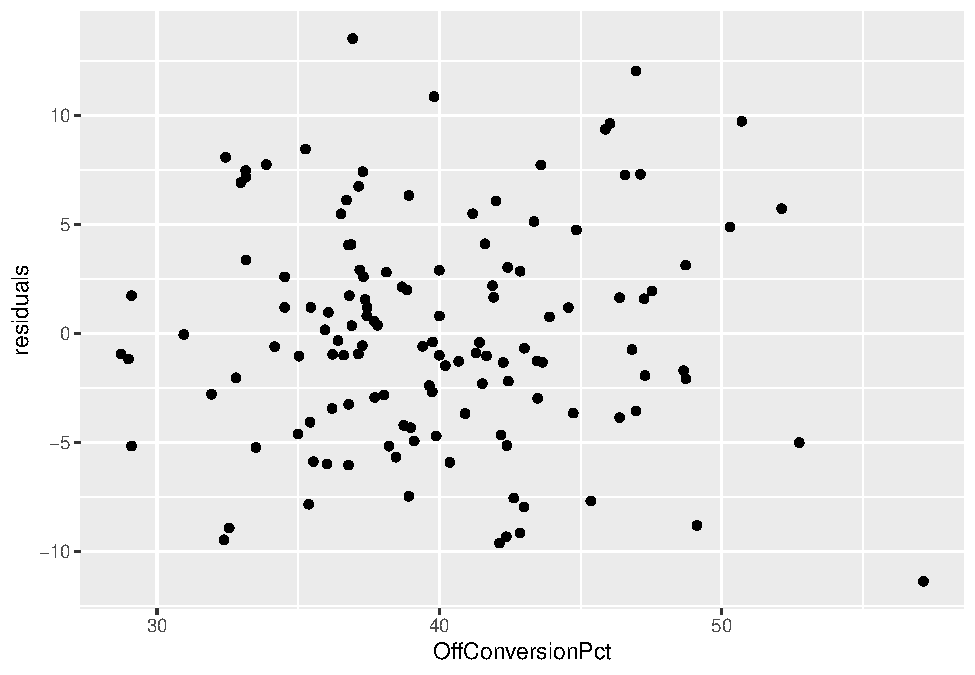
\includegraphics{SportsData_files/figure-latex/unnamed-chunk-87-1.pdf}

The lack of a shape here -- the seemingly random nature -- is a good
sign that a linear model works for our data. If there was a pattern,
that would indicate something else was going on in our data and we
needed a different model.

Another way to view your residuals is by connecting the predicted value
with the actual value.

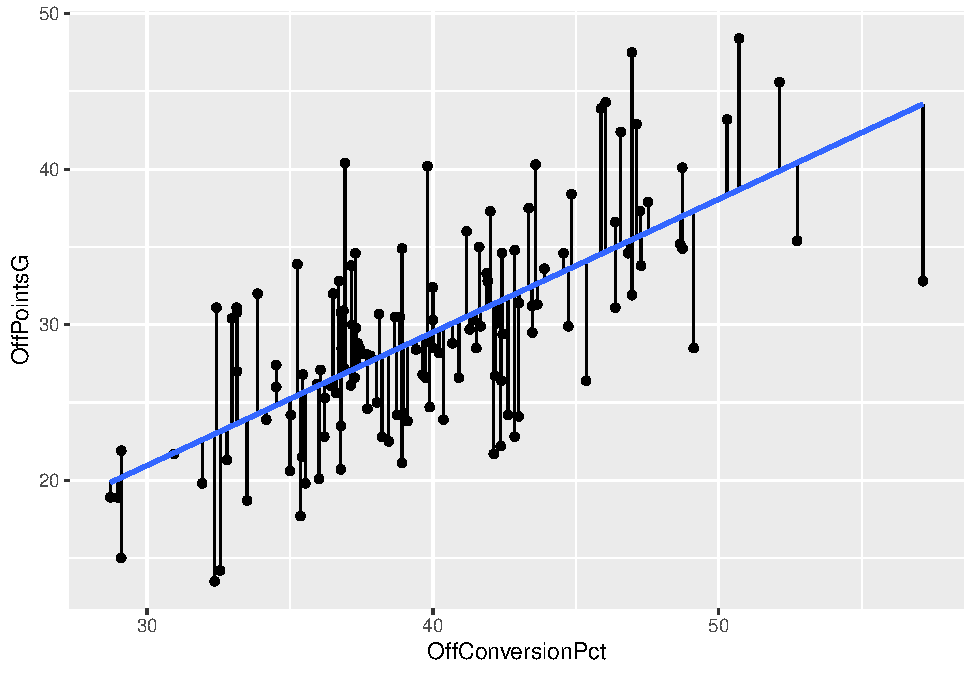
\includegraphics{SportsData_files/figure-latex/unnamed-chunk-88-1.pdf}

The blue line here separates underperformers from overperformers.

\section{Penalties}\label{penalties}

Now let's look at it where it doesn't work: Penalties.

\begin{Shaded}
\begin{Highlighting}[]
\NormalTok{penalties <-}\StringTok{ }\NormalTok{offense}
\end{Highlighting}
\end{Shaded}

\begin{Shaded}
\begin{Highlighting}[]
\NormalTok{pfit <-}\StringTok{ }\KeywordTok{lm}\NormalTok{(OffPointsG }\OperatorTok{~}\StringTok{ }\NormalTok{Yards, }\DataTypeTok{data =}\NormalTok{ penalties)}
\KeywordTok{summary}\NormalTok{(pfit)}
\end{Highlighting}
\end{Shaded}

\begin{verbatim}
## 
## Call:
## lm(formula = OffPointsG ~ Yards, data = penalties)
## 
## Residuals:
##      Min       1Q   Median       3Q      Max 
## -16.5381  -4.5779  -0.5204   4.2418  17.0543 
## 
## Coefficients:
##              Estimate Std. Error t value Pr(>|t|)    
## (Intercept) 20.897213   2.819227   7.412 1.49e-11 ***
## Yards        0.012220   0.003966   3.082  0.00252 ** 
## ---
## Signif. codes:  0 '***' 0.001 '**' 0.01 '*' 0.05 '.' 0.1 ' ' 1
## 
## Residual standard error: 6.61 on 128 degrees of freedom
## Multiple R-squared:  0.06907,    Adjusted R-squared:  0.06179 
## F-statistic: 9.496 on 1 and 128 DF,  p-value: 0.002521
\end{verbatim}

So from top to bottom:

\begin{itemize}
\tightlist
\item
  Our min and max go from -16.5 to positive 17.1
\item
  Our adjusted R-squared is \ldots{} .06. Not much at all.
\item
  Our p-value is \ldots{} .002, which is less than than .05.
\end{itemize}

So what we can say about this model is that it's statistically
significant but utterly meaningless. Normally, we'd stop right here --
why bother going forward with a predictive model that isn't predictive?
But let's do it anyway.

\begin{Shaded}
\begin{Highlighting}[]
\NormalTok{penalties}\OperatorTok{$}\NormalTok{predicted <-}\StringTok{ }\KeywordTok{predict}\NormalTok{(pfit)}
\NormalTok{penalties}\OperatorTok{$}\NormalTok{residuals <-}\StringTok{ }\KeywordTok{residuals}\NormalTok{(pfit)}
\end{Highlighting}
\end{Shaded}

\begin{Shaded}
\begin{Highlighting}[]
\NormalTok{penalties }\OperatorTok\StringTok{ }\KeywordTok{arrange}\NormalTok{(}\KeywordTok{desc}\NormalTok{(residuals))}
\end{Highlighting}
\end{Shaded}

\begin{verbatim}
## # A tibble: 130 x 14
##    Name  OffPoints OffPointsG DefPoints DefPointsG  Pen. Yards `Pen./G`
##    <chr>     <dbl>      <dbl>     <dbl>      <dbl> <dbl> <dbl>    <dbl>
##  1 Okla~       677       48.4       466       33.3    86   855      6.1
##  2 Utah~       618       47.5       289       22.2   101   916      7.8
##  3 Clem~       664       44.3       197       13.1    73   674      4.9
##  4 Alab~       684       45.6       271       18.1    87   796      5.8
##  5 Hous~       571       43.9       483       37.2    87   683      6.7
##  6 UCF         562       43.2       295       22.7    97   848      7.5
##  7 Memp~       601       42.9       447       31.9   101   833      7.2
##  8 Ohio        521       40.1       320       24.6    64   652      4.9
##  9 Syra~       523       40.2       351       27      94   768      7.2
## 10 West~       483       40.3       326       27.2    85   800      7.1
## # ... with 120 more rows, and 6 more variables: OffConversions <dbl>,
## #   OffConversionPct <dbl>, DefConversions <dbl>, DefConversionPct <dbl>,
## #   predicted <dbl>, residuals <dbl>
\end{verbatim}

So our model says Oklahoma \emph{should} only be scoring 31.3 points per
game given how many penalty yards per game, but they're really scoring
48.4. Oy. What happens if we plot those residuals?

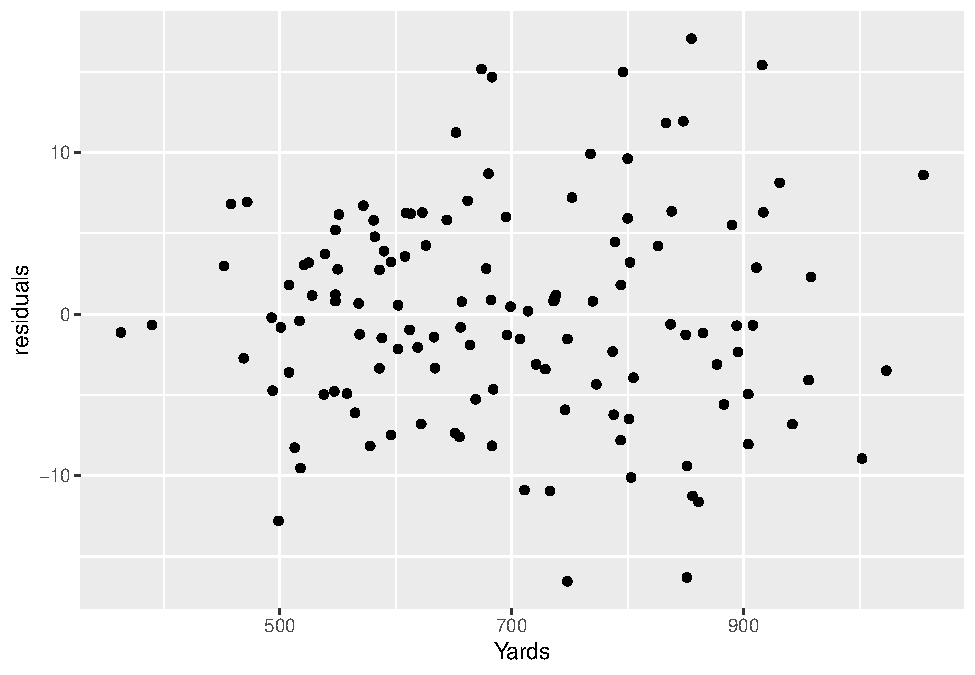
\includegraphics{SportsData_files/figure-latex/unnamed-chunk-93-1.pdf}

Well \ldots{} it actually says that a linear model is appropriate. Which
an important lesson -- just because your residual plot says a linear
model works here, that doesn't say your linear model is good. There are
other measures for that, and you need to use them.

Here's the segment plot of residuals -- you'll see some really long
lines. That's a bad sign.

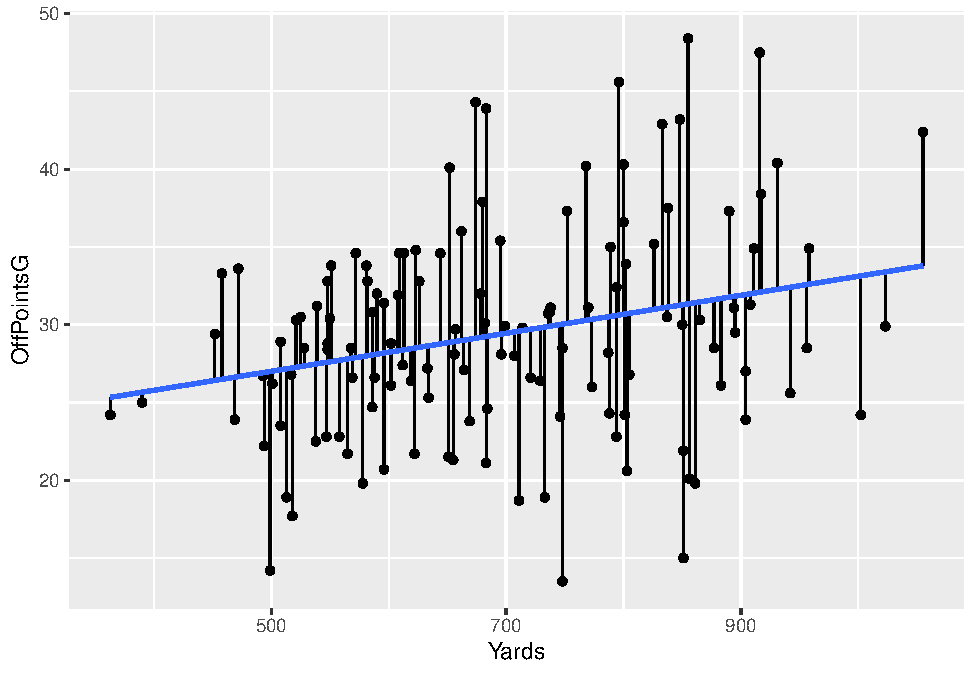
\includegraphics{SportsData_files/figure-latex/unnamed-chunk-94-1.pdf}

\chapter{Z scores}\label{z-scores}

Z scores are a handy way to standardize scores so you can compare things
across groupings. In our case, we may want to compare teams by year, or
era. We can use z scores to answer questions like who was the greatest X
of all time, because a Z score can put them in context to their era.

We can also use z scores to ask how much better is team A from team B.

So let's use Nebraska basketball, which if you haven't been reading
lately is at a bit of a crossroads.

A Z score is a measure of how far a number is from the population mean
of that number. An easier way to say that -- how different is my grade
from the average grade in the class. The formula for calculating a Z
score is
\texttt{(MyScore\ -\ AverageScore)/Standard\ Deviation\ of\ Scores}. The
standard deviation is a number calculated to show the amount of
variation in a set of data. In a normal distribution, 68 percent of all
scores will be within 1 standard deviation, 95 percent will be within 2
and 99 within 3.

\section{Calculating a Z score in R}\label{calculating-a-z-score-in-r}

\begin{Shaded}
\begin{Highlighting}[]
\KeywordTok{library}\NormalTok{(tidyverse)}
\end{Highlighting}
\end{Shaded}

\begin{Shaded}
\begin{Highlighting}[]
\NormalTok{gamelogs <-}\StringTok{ }\KeywordTok{read_csv}\NormalTok{(}\StringTok{"data/logs19.csv"}\NormalTok{)}
\end{Highlighting}
\end{Shaded}

\begin{verbatim}
## Warning: Missing column names filled in: 'X1' [1]
\end{verbatim}

\begin{verbatim}
## Parsed with column specification:
## cols(
##   .default = col_double(),
##   Date = col_date(format = ""),
##   HomeAway = col_character(),
##   Opponent = col_character(),
##   W_L = col_character(),
##   Blank = col_logical(),
##   Team = col_character(),
##   Conference = col_character(),
##   season = col_character()
## )
\end{verbatim}

\begin{verbatim}
## See spec(...) for full column specifications.
\end{verbatim}

The first thing we need to do is select some fields we think represent
team quality:

\begin{Shaded}
\begin{Highlighting}[]
\NormalTok{teamquality <-}\StringTok{ }\NormalTok{gamelogs }\OperatorTok\StringTok{ }\KeywordTok{select}\NormalTok{(Conference, Team, TeamFGPCT, TeamTotalRebounds, OpponentFGPCT)}
\end{Highlighting}
\end{Shaded}

And since we have individual game data, we need to collapse this into
one record for each team. We do that with \ldots{} group by.

\begin{Shaded}
\begin{Highlighting}[]
\NormalTok{teamtotals <-}\StringTok{ }\NormalTok{teamquality }\OperatorTok\StringTok{ }
\StringTok{  }\KeywordTok{group_by}\NormalTok{(Conference, Team) }\OperatorTok\StringTok{ }
\StringTok{  }\KeywordTok{summarise}\NormalTok{(}
    \DataTypeTok{FGAvg =} \KeywordTok{mean}\NormalTok{(TeamFGPCT), }
    \DataTypeTok{ReboundAvg =} \KeywordTok{mean}\NormalTok{(TeamTotalRebounds), }
    \DataTypeTok{OppFGAvg =} \KeywordTok{mean}\NormalTok{(OpponentFGPCT)}
\NormalTok{    )}
\end{Highlighting}
\end{Shaded}

To calculate a Z score in R, the easiest way is to use the scale
function in base R. To use it, you use
\texttt{scale(FieldName,\ center=TRUE,\ scale=TRUE)}. The center and
scale indicate if you want to subtract from the mean and if you want to
divide by the standard deviation, respectively. We do.

When we have multiple Z Scores, it's pretty standard practice to add
them together into a composite score. That's what we're doing at the end
here with \texttt{TotalZscore}. Note: We have to invert OppZscore by
multiplying it by a negative 1 because the lower someone's opponent
shooting percentage is, the better.

\begin{Shaded}
\begin{Highlighting}[]
\NormalTok{teamzscore <-}\StringTok{ }\NormalTok{teamtotals }\OperatorTok\StringTok{ }\KeywordTok{mutate}\NormalTok{(}
  \DataTypeTok{FGzscore =} \KeywordTok{as.numeric}\NormalTok{(}\KeywordTok{scale}\NormalTok{(FGAvg, }\DataTypeTok{center =} \OtherTok{TRUE}\NormalTok{, }\DataTypeTok{scale =} \OtherTok{TRUE}\NormalTok{)),}
  \DataTypeTok{RebZscore =} \KeywordTok{as.numeric}\NormalTok{(}\KeywordTok{scale}\NormalTok{(ReboundAvg, }\DataTypeTok{center =} \OtherTok{TRUE}\NormalTok{, }\DataTypeTok{scale =} \OtherTok{TRUE}\NormalTok{)),}
  \DataTypeTok{OppZscore =} \KeywordTok{as.numeric}\NormalTok{(}\KeywordTok{scale}\NormalTok{(OppFGAvg, }\DataTypeTok{center =} \OtherTok{TRUE}\NormalTok{, }\DataTypeTok{scale =} \OtherTok{TRUE}\NormalTok{)) }\OperatorTok{*}\StringTok{ }\OperatorTok{-}\DecValTok{1}\NormalTok{,}
  \DataTypeTok{TotalZscore =}\NormalTok{ FGzscore }\OperatorTok{+}\StringTok{ }\NormalTok{RebZscore }\OperatorTok{+}\StringTok{ }\NormalTok{OppZscore}
\NormalTok{  )  }
\end{Highlighting}
\end{Shaded}

So now we have a dataframe called \texttt{teamzscore} that has 353
basketball teams with Z scores. What does it look like?

\begin{Shaded}
\begin{Highlighting}[]
\KeywordTok{head}\NormalTok{(teamzscore)}
\end{Highlighting}
\end{Shaded}

\begin{verbatim}
## # A tibble: 6 x 9
## # Groups:   Conference [1]
##   Conference Team  FGAvg ReboundAvg OppFGAvg FGzscore RebZscore OppZscore
##   <chr>      <chr> <dbl>      <dbl>    <dbl>    <dbl>     <dbl>     <dbl>
## 1 A-10       Davi~ 0.453       32.2    0.409    0.606    0.106      1.000
## 2 A-10       Dayt~ 0.506       32.1    0.415    2.42     0.0525     0.753
## 3 A-10       Duqu~ 0.427       32.7    0.444   -0.286    0.339     -0.511
## 4 A-10       Ford~ 0.402       31      0.436   -1.12    -0.432     -0.169
## 5 A-10       Geor~ 0.443       32      0.441    0.278    0.0248    -0.380
## 6 A-10       Geor~ 0.409       31.3    0.445   -0.891   -0.308     -0.559
## # ... with 1 more variable: TotalZscore <dbl>
\end{verbatim}

A way to read this -- a team at zero is precisely average. The larger
the positive number, the more exceptional they are. The larger the
negative number, the more truly terrible they are.

So who are the best teams in the country?

\begin{Shaded}
\begin{Highlighting}[]
\NormalTok{teamzscore }\OperatorTok\StringTok{ }\KeywordTok{arrange}\NormalTok{(}\KeywordTok{desc}\NormalTok{(TotalZscore))}
\end{Highlighting}
\end{Shaded}

\begin{verbatim}
## # A tibble: 353 x 9
## # Groups:   Conference [32]
##    Conference Team  FGAvg ReboundAvg OppFGAvg FGzscore RebZscore OppZscore
##    <chr>      <chr> <dbl>      <dbl>    <dbl>    <dbl>     <dbl>     <dbl>
##  1 WCC        Gonz~ 0.531       36.3    0.386    2.25      2.02       2.23
##  2 Big Ten    Mich~ 0.486       38.1    0.378    2.13      2.22       1.86
##  3 Summit     Sout~ 0.501       35.1    0.419    1.89      1.68       2.27
##  4 Ivy        Yale~ 0.494       36.2    0.414    1.84      1.80       1.42
##  5 AAC        Hous~ 0.447       37.2    0.370    0.530     2.14       2.22
##  6 SEC        Kent~ 0.479       36.2    0.399    1.31      1.48       2.08
##  7 SEC        Tenn~ 0.496       34.7    0.400    2.08      0.775      2.01
##  8 SWAC       Gram~ 0.451       34.7    0.395    1.18      1.19       2.26
##  9 Big West   UC-I~ 0.457       36.5    0.382    0.774     1.55       2.29
## 10 OVC        Belm~ 0.501       36.2    0.423    1.91      1.46       1.09
## # ... with 343 more rows, and 1 more variable: TotalZscore <dbl>
\end{verbatim}

Don't sleep on South Dakota State come tournament time!

But closer to home, how is Nebraska doing.

\begin{Shaded}
\begin{Highlighting}[]
\NormalTok{teamzscore }\OperatorTok\StringTok{ }\KeywordTok{filter}\NormalTok{(Conference }\OperatorTok{==}\StringTok{ "Big Ten"}\NormalTok{) }\OperatorTok\StringTok{ }\KeywordTok{arrange}\NormalTok{(}\KeywordTok{desc}\NormalTok{(TotalZscore))}
\end{Highlighting}
\end{Shaded}

\begin{verbatim}
## # A tibble: 14 x 9
## # Groups:   Conference [1]
##    Conference Team  FGAvg ReboundAvg OppFGAvg FGzscore RebZscore OppZscore
##    <chr>      <chr> <dbl>      <dbl>    <dbl>    <dbl>     <dbl>     <dbl>
##  1 Big Ten    Mich~ 0.486       38.1    0.378    2.13     2.22     1.86   
##  2 Big Ten    Mary~ 0.451       36.1    0.398    0.439    1.31     0.996  
##  3 Big Ten    Mich~ 0.451       32.4    0.397    0.480   -0.414    1.02   
##  4 Big Ten    Wisc~ 0.450       32.4    0.397    0.421   -0.430    1.01   
##  5 Big Ten    Purd~ 0.450       34.1    0.416    0.421    0.354    0.218  
##  6 Big Ten    Indi~ 0.460       33.4    0.421    0.911    0.0431   0.0192 
##  7 Big Ten    Rutg~ 0.419       35.9    0.425   -1.06     1.20    -0.147  
##  8 Big Ten    Iowa~ 0.457       32.7    0.450    0.726   -0.251   -1.22   
##  9 Big Ten    Nebr~ 0.431       32.5    0.423   -0.509   -0.363   -0.0525 
## 10 Big Ten    Ohio~ 0.436       31.9    0.426   -0.264   -0.632   -0.185  
## 11 Big Ten    Minn~ 0.435       32.7    0.439   -0.277   -0.261   -0.757  
## 12 Big Ten    Penn~ 0.418       33.1    0.442   -1.09    -0.0897  -0.891  
## 13 Big Ten    Nort~ 0.403       30.9    0.421   -1.84    -1.10     0.00345
## 14 Big Ten    Illi~ 0.431       29.8    0.466   -0.489   -1.60    -1.88   
## # ... with 1 more variable: TotalZscore <dbl>
\end{verbatim}

So, as we can see, with our composite Z Score, Nebraska is \ldots{} not
bad, but not good either: 9 of 14 teams in the Big Ten.

\chapter{Intro to ggplot}\label{intro-to-ggplot}

With \texttt{ggplot2}, we dive into the world of programmatic data
visualization. The \texttt{ggplot2} library implements something called
the grammar of graphics. The main concepts are:

\begin{itemize}
\tightlist
\item
  aesthetics - which in this case means the data which we are going to
  plot
\item
  geometries - which means the shape the data is going to take
\item
  scales - which means any transformations we might make on the data
\item
  facets - which means how we might graph many elements of the same
  dataset in the same space
\item
  layers - which means how we might lay multiple geometries over top of
  each other to reveal new information.
\end{itemize}

Hadley Wickam, who is behind all of the libaries we have used in this
course to date, wrote about his layered grammar of graphics in
\href{http://byrneslab.net/classes/biol607/readings/wickham_layered-grammar.pdf}{this
2009 paper that is worth your time to read}.

Here are some \texttt{ggplot2} resources you'll want to keep handy:

\begin{itemize}
\tightlist
\item
  \href{http://ggplot2.tidyverse.org/reference/index.html}{The ggplot
  documentation}.
\item
  \href{http://www.cookbook-r.com/Graphs/}{The ggplot cookbook}
\end{itemize}

Let's dive in using data we've already seen before -- football
attendance. This workflow will represent a clear picture of what your
work in this class will be like for much of the rest of the semester.
One way to think of this workflow is that your R Notebook is now your
digital sketchbook, where you will try different types of visualizations
to find ones that work. Then, you will export your work into a program
like Illustrator to finish the work.

To begin, we'll import the \texttt{ggplot2} and \texttt{dplyr}
libraries. We'll read in the data, then create a new dataframe that
represents our attendance data, similar to what we've done before.

\begin{Shaded}
\begin{Highlighting}[]
\KeywordTok{library}\NormalTok{(tidyverse)}
\end{Highlighting}
\end{Shaded}

\begin{Shaded}
\begin{Highlighting}[]
\NormalTok{attendance <-}\StringTok{ }\KeywordTok{read_csv}\NormalTok{(}\StringTok{'data/attendance.csv'}\NormalTok{)}
\end{Highlighting}
\end{Shaded}

\begin{verbatim}
## Parsed with column specification:
## cols(
##   Institution = col_character(),
##   Conference = col_character(),
##   `2013` = col_double(),
##   `2014` = col_double(),
##   `2015` = col_double(),
##   `2016` = col_double(),
##   `2017` = col_double(),
##   `2018` = col_double()
## )
\end{verbatim}

First, let's get a top 10 list by announced attendance this last season.
We'll use the same tricks we used in the filtering assignment.

\begin{Shaded}
\begin{Highlighting}[]
\NormalTok{attendance }\OperatorTok\StringTok{ }\KeywordTok{arrange}\NormalTok{(}\KeywordTok{desc}\NormalTok{(}\StringTok{`}\DataTypeTok{2018}\StringTok{`}\NormalTok{)) }\OperatorTok\StringTok{ }\KeywordTok{top_n}\NormalTok{(}\DecValTok{10}\NormalTok{) }\OperatorTok\StringTok{ }\KeywordTok{select}\NormalTok{(Institution, }\StringTok{`}\DataTypeTok{2018}\StringTok{`}\NormalTok{)}
\end{Highlighting}
\end{Shaded}

\begin{verbatim}
## Selecting by 2018
\end{verbatim}

\begin{verbatim}
## # A tibble: 10 x 2
##    Institution `2018`
##    <chr>        <dbl>
##  1 Michigan    775156
##  2 Penn St.    738396
##  3 Ohio St.    713630
##  4 Alabama     710931
##  5 LSU         705733
##  6 Texas A&M   698908
##  7 Tennessee   650887
##  8 Georgia     649222
##  9 Nebraska    623240
## 10 Oklahoma    607146
\end{verbatim}

That looks good, so let's save it to a new data frame and use that data
frame instead going forward.

\begin{Shaded}
\begin{Highlighting}[]
\NormalTok{top10 <-}\StringTok{ }\NormalTok{attendance }\OperatorTok\StringTok{ }\KeywordTok{arrange}\NormalTok{(}\KeywordTok{desc}\NormalTok{(}\StringTok{`}\DataTypeTok{2018}\StringTok{`}\NormalTok{)) }\OperatorTok\StringTok{ }\KeywordTok{top_n}\NormalTok{(}\DecValTok{10}\NormalTok{) }\OperatorTok\StringTok{ }\KeywordTok{select}\NormalTok{(Institution, }\StringTok{`}\DataTypeTok{2018}\StringTok{`}\NormalTok{)}
\end{Highlighting}
\end{Shaded}

\begin{verbatim}
## Selecting by 2018
\end{verbatim}

The easiest thing we can do is create a simple bar chart of our data. We
could, for instance, create a bar chart of the total attendance. To do
that, we simply tell \texttt{ggplot2} what our dataset is, what element
of the data we want to make the bar chart out of (which is the
aesthetic), and the geometry type (which is the geom). It looks like
this:

\texttt{ggplot(top10,\ aes(x=Institution))\ +\ geom\_bar()}

Note: attendace is our data, \texttt{aes} means aesthetics,
\texttt{x=Institution} explicitly tells \texttt{ggplot2} that our x
value -- our horizontal value -- is the Instituition field from the
data, and then we add on the \texttt{geom\_bar()} as the geometry. And
what do we get when we run that?

\begin{Shaded}
\begin{Highlighting}[]
\KeywordTok{ggplot}\NormalTok{(top10, }\KeywordTok{aes}\NormalTok{(}\DataTypeTok{x=}\NormalTok{Institution)) }\OperatorTok{+}\StringTok{ }\KeywordTok{geom_bar}\NormalTok{()}
\end{Highlighting}
\end{Shaded}

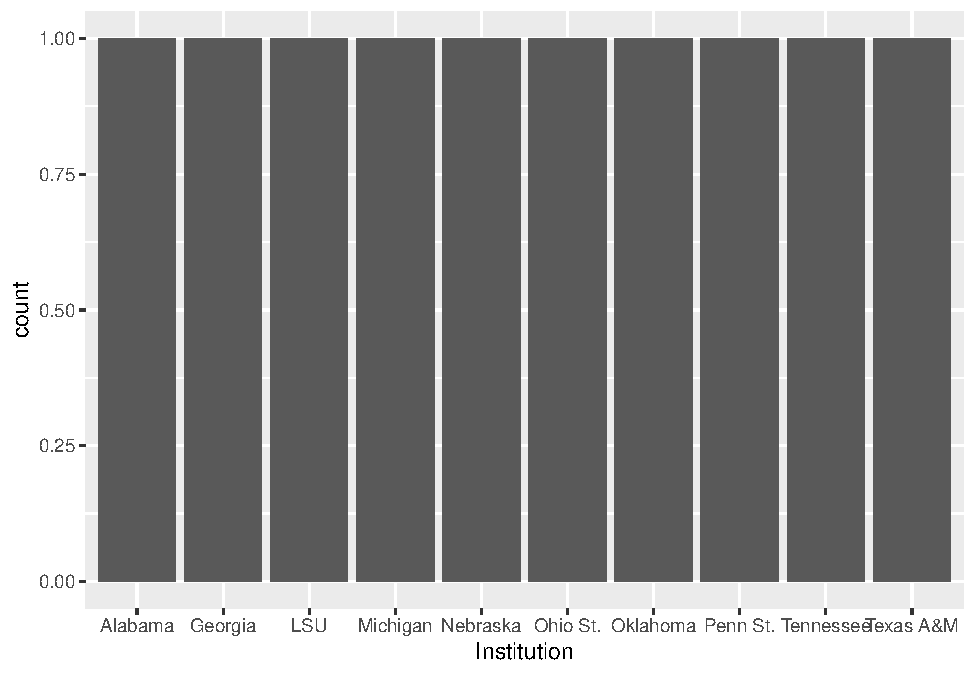
\includegraphics{SportsData_files/figure-latex/unnamed-chunk-107-1.pdf}

We get \ldots{} weirdness. We expected to see bars of different sizes,
but we get all with a count of 1. What gives? Well, this is the default
behavior. What we have here is something called a histogram, where
\texttt{ggplot2} helpfully counted up the number of times the
Institution appears and counted them up. Since we only have one record
per Institution, the count is always 1. How do we fix this? By adding
\texttt{weight} to our aesthetic.

\begin{Shaded}
\begin{Highlighting}[]
\KeywordTok{ggplot}\NormalTok{(top10, }\KeywordTok{aes}\NormalTok{(}\DataTypeTok{x=}\NormalTok{Institution, }\DataTypeTok{weight=}\StringTok{`}\DataTypeTok{2018}\StringTok{`}\NormalTok{)) }\OperatorTok{+}\StringTok{ }\KeywordTok{geom_bar}\NormalTok{()}
\end{Highlighting}
\end{Shaded}

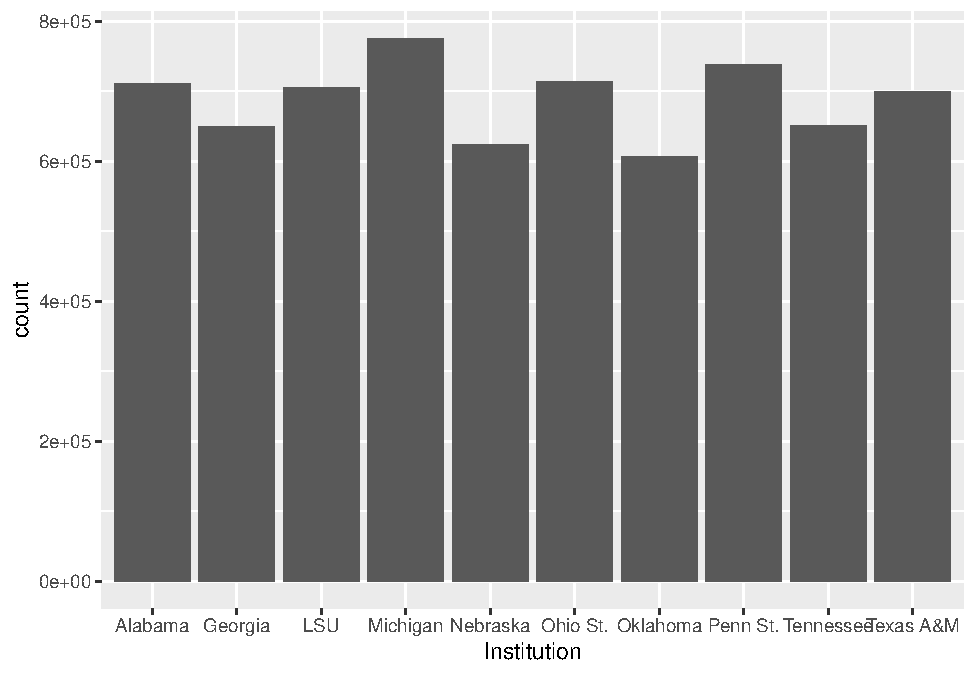
\includegraphics{SportsData_files/figure-latex/unnamed-chunk-108-1.pdf}

Closer. But \ldots{} what order is that in? And what happened to our
count numbers on the left? Why are they in scientific notation?

Let's deal with the ordering first. \texttt{ggplot2}'s default behavior
is to sort the data by the x axis variable. So it's in alphabetical
order. To change that, we have to \texttt{reorder} it. With
\texttt{reorder}, we first have to tell \texttt{ggplot} what we are
reordering, and then we have to tell it HOW we are reordering it. So
it's reorder(FIELD, SORTFIELD).

\begin{Shaded}
\begin{Highlighting}[]
\KeywordTok{ggplot}\NormalTok{(top10, }\KeywordTok{aes}\NormalTok{(}\DataTypeTok{x=}\KeywordTok{reorder}\NormalTok{(Institution, }\StringTok{`}\DataTypeTok{2018}\StringTok{`}\NormalTok{), }\DataTypeTok{weight=}\StringTok{`}\DataTypeTok{2018}\StringTok{`}\NormalTok{)) }\OperatorTok{+}\StringTok{ }\KeywordTok{geom_bar}\NormalTok{()}
\end{Highlighting}
\end{Shaded}

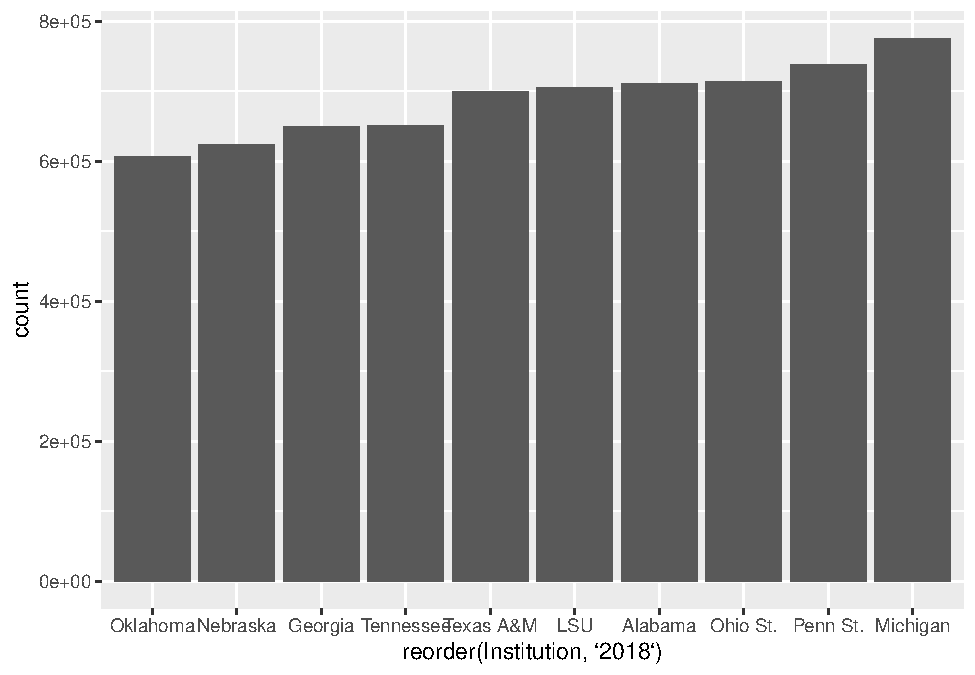
\includegraphics{SportsData_files/figure-latex/unnamed-chunk-109-1.pdf}

Better. We can argue about if the right order is smallest to largest or
largest to smallest. But this gets us close. By the way, to sort it
largest to smallest, put a negative sign in front of the sort field.

\begin{Shaded}
\begin{Highlighting}[]
\KeywordTok{ggplot}\NormalTok{(top10, }\KeywordTok{aes}\NormalTok{(}\DataTypeTok{x=}\KeywordTok{reorder}\NormalTok{(Institution, }\OperatorTok{-}\StringTok{`}\DataTypeTok{2018}\StringTok{`}\NormalTok{), }\DataTypeTok{weight=}\StringTok{`}\DataTypeTok{2018}\StringTok{`}\NormalTok{)) }\OperatorTok{+}\StringTok{ }\KeywordTok{geom_bar}\NormalTok{()}
\end{Highlighting}
\end{Shaded}

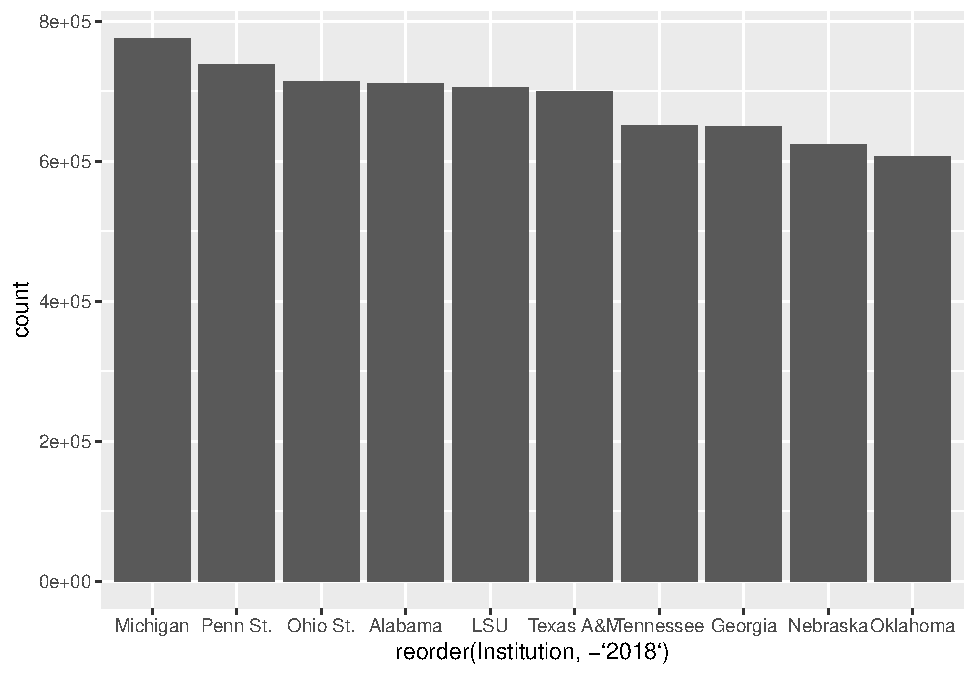
\includegraphics{SportsData_files/figure-latex/unnamed-chunk-110-1.pdf}

\section{Scales}\label{scales}

To fix the axis labels, we need try one of the other main elements of
the \texttt{ggplot2} library, which is transform a scale. More often
that not, that means doing something like putting it on a logarithmic
scale or soem other kind of transformation. In this case, we're just
changing how it's represented. The default in \texttt{ggplot2} for large
values is to express them as scientific notation. Rarely ever is that
useful in our line of work. So we have to transform them into human
readable numbers.

The easiest way to do this is to use a library called \texttt{scales}
and it's already installed.

\begin{Shaded}
\begin{Highlighting}[]
\KeywordTok{library}\NormalTok{(scales)}
\end{Highlighting}
\end{Shaded}

To alter the scale, we add a piece to our plot with \texttt{+} and we
tell it which scale is getting altered and what kind of data it is. In
our case, our Y axis is what is needing to be altered, and it's
continuous data (meaning it can be any number between x and y, vs
discrete data which are categorical). So we need to add
\texttt{scale\_y\_continuous} and the information we want to pass it is
to alter the labels with a function called \texttt{comma}.

\begin{Shaded}
\begin{Highlighting}[]
\KeywordTok{ggplot}\NormalTok{(top10, }\KeywordTok{aes}\NormalTok{(}\DataTypeTok{x=}\KeywordTok{reorder}\NormalTok{(Institution, }\OperatorTok{-}\StringTok{`}\DataTypeTok{2018}\StringTok{`}\NormalTok{), }\DataTypeTok{weight=}\StringTok{`}\DataTypeTok{2018}\StringTok{`}\NormalTok{)) }\OperatorTok{+}\StringTok{ }\KeywordTok{geom_bar}\NormalTok{() }\OperatorTok{+}\StringTok{ }\KeywordTok{scale_y_continuous}\NormalTok{(}\DataTypeTok{labels=}\NormalTok{comma)}
\end{Highlighting}
\end{Shaded}

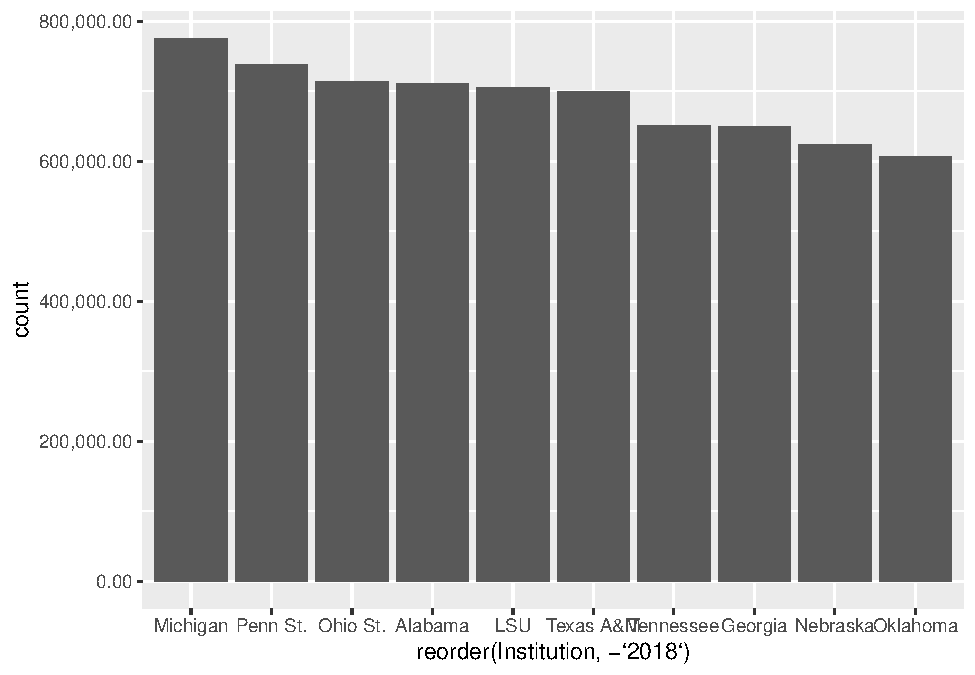
\includegraphics{SportsData_files/figure-latex/unnamed-chunk-112-1.pdf}

Better.

\section{Styling}\label{styling}

We are going to spend a lot more time on styling, but let's add some
simple labels to this with a new bit called \texttt{labs} which is short
for labels.

\begin{Shaded}
\begin{Highlighting}[]
\KeywordTok{ggplot}\NormalTok{(top10, }\KeywordTok{aes}\NormalTok{(}\DataTypeTok{x=}\KeywordTok{reorder}\NormalTok{(Institution, }\OperatorTok{-}\StringTok{`}\DataTypeTok{2018}\StringTok{`}\NormalTok{), }\DataTypeTok{weight=}\StringTok{`}\DataTypeTok{2018}\StringTok{`}\NormalTok{)) }\OperatorTok{+}\StringTok{ }\KeywordTok{geom_bar}\NormalTok{() }\OperatorTok{+}\StringTok{ }\KeywordTok{scale_y_continuous}\NormalTok{(}\DataTypeTok{labels=}\NormalTok{comma) }\OperatorTok{+}\StringTok{ }\KeywordTok{labs}\NormalTok{(}\DataTypeTok{title=}\StringTok{"Top 10 Football Programs By Attendance"}\NormalTok{, }\DataTypeTok{x=}\StringTok{"School"}\NormalTok{, }\DataTypeTok{y=}\StringTok{"Attendance"}\NormalTok{)}
\end{Highlighting}
\end{Shaded}

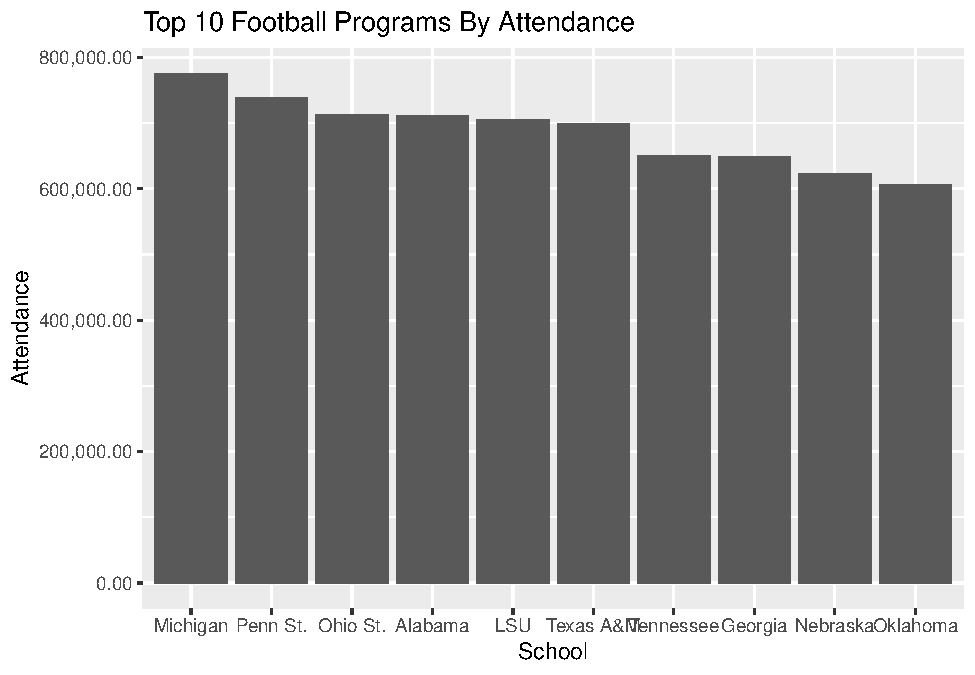
\includegraphics{SportsData_files/figure-latex/unnamed-chunk-113-1.pdf}

The library has lots and lots of ways to alter the styling -- we can
programmatically control nearly every part of the look and feel of the
chart. One simple way is to apply themes in the library already. We do
that the same way we've done other things -- we add them. Here's the
light theme.

\begin{Shaded}
\begin{Highlighting}[]
\KeywordTok{ggplot}\NormalTok{(top10, }\KeywordTok{aes}\NormalTok{(}\DataTypeTok{x=}\KeywordTok{reorder}\NormalTok{(Institution, }\OperatorTok{-}\StringTok{`}\DataTypeTok{2018}\StringTok{`}\NormalTok{), }\DataTypeTok{weight=}\StringTok{`}\DataTypeTok{2018}\StringTok{`}\NormalTok{)) }\OperatorTok{+}\StringTok{ }\KeywordTok{geom_bar}\NormalTok{() }\OperatorTok{+}\StringTok{ }\KeywordTok{scale_y_continuous}\NormalTok{(}\DataTypeTok{labels=}\NormalTok{comma) }\OperatorTok{+}\StringTok{ }\KeywordTok{labs}\NormalTok{(}\DataTypeTok{title=}\StringTok{"Top 10 Football Programs By Attendance"}\NormalTok{, }\DataTypeTok{x=}\StringTok{"School"}\NormalTok{, }\DataTypeTok{y=}\StringTok{"Attendance"}\NormalTok{) }\OperatorTok{+}\StringTok{ }\KeywordTok{theme_light}\NormalTok{()}
\end{Highlighting}
\end{Shaded}

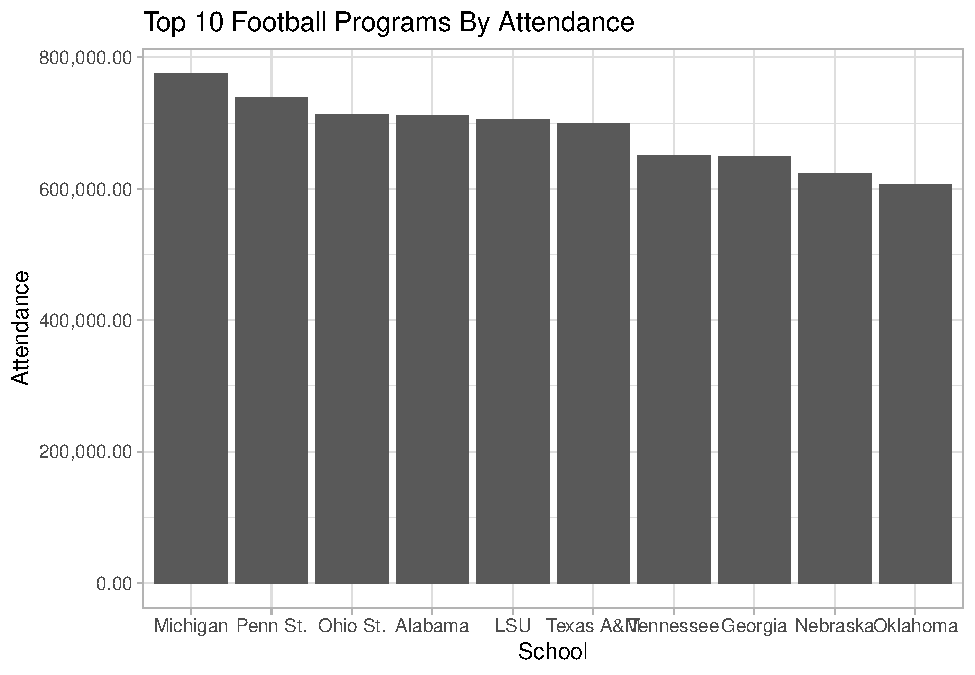
\includegraphics{SportsData_files/figure-latex/unnamed-chunk-114-1.pdf}

Or the minimal theme:

\begin{Shaded}
\begin{Highlighting}[]
\KeywordTok{ggplot}\NormalTok{(top10, }\KeywordTok{aes}\NormalTok{(}\DataTypeTok{x=}\KeywordTok{reorder}\NormalTok{(Institution, }\OperatorTok{-}\StringTok{`}\DataTypeTok{2018}\StringTok{`}\NormalTok{), }\DataTypeTok{weight=}\StringTok{`}\DataTypeTok{2018}\StringTok{`}\NormalTok{)) }\OperatorTok{+}\StringTok{ }\KeywordTok{geom_bar}\NormalTok{() }\OperatorTok{+}\StringTok{ }\KeywordTok{scale_y_continuous}\NormalTok{(}\DataTypeTok{labels=}\NormalTok{comma) }\OperatorTok{+}\StringTok{ }\KeywordTok{labs}\NormalTok{(}\DataTypeTok{title=}\StringTok{"Top 10 Football Programs By Attendance"}\NormalTok{, }\DataTypeTok{x=}\StringTok{"School"}\NormalTok{, }\DataTypeTok{y=}\StringTok{"Attendance"}\NormalTok{) }\OperatorTok{+}\StringTok{ }\KeywordTok{theme_minimal}\NormalTok{()}
\end{Highlighting}
\end{Shaded}

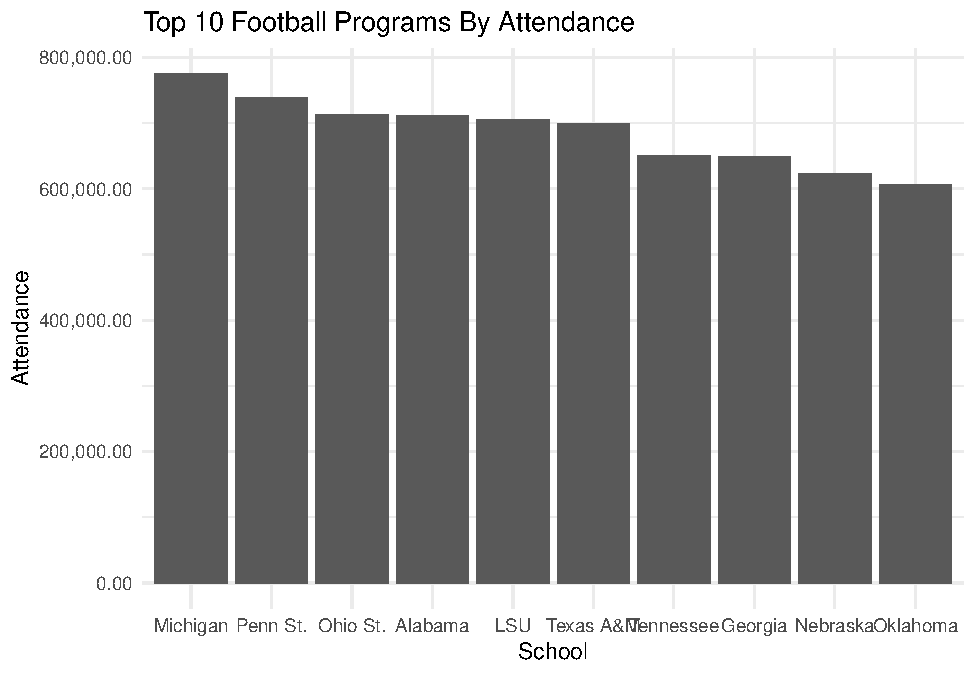
\includegraphics{SportsData_files/figure-latex/unnamed-chunk-115-1.pdf}

Later on, we'll write our own themes. For now, the built in ones will
get us closer to something that looks good.

\section{One last trick: coord flip}\label{one-last-trick-coord-flip}

Sometimes, we don't want vertical bars. Maybe we think this would look
better horizontal. How do we do that? By adding \texttt{coord\_flip()}
to our code. It does what it says -- it inverts the coordinates of the
figures.

\begin{Shaded}
\begin{Highlighting}[]
\KeywordTok{ggplot}\NormalTok{(top10, }\KeywordTok{aes}\NormalTok{(}\DataTypeTok{x=}\KeywordTok{reorder}\NormalTok{(Institution, }\OperatorTok{-}\StringTok{`}\DataTypeTok{2018}\StringTok{`}\NormalTok{), }\DataTypeTok{weight=}\StringTok{`}\DataTypeTok{2018}\StringTok{`}\NormalTok{)) }\OperatorTok{+}\StringTok{ }\KeywordTok{geom_bar}\NormalTok{() }\OperatorTok{+}\StringTok{ }\KeywordTok{scale_y_continuous}\NormalTok{(}\DataTypeTok{labels=}\NormalTok{comma) }\OperatorTok{+}\StringTok{ }\KeywordTok{labs}\NormalTok{(}\DataTypeTok{title=}\StringTok{"Top 10 Football Programs By Attendance"}\NormalTok{, }\DataTypeTok{x=}\StringTok{"School"}\NormalTok{, }\DataTypeTok{y=}\StringTok{"Attendance"}\NormalTok{) }\OperatorTok{+}\StringTok{ }\KeywordTok{theme_minimal}\NormalTok{() }\OperatorTok{+}\StringTok{ }\KeywordTok{coord_flip}\NormalTok{()}
\end{Highlighting}
\end{Shaded}

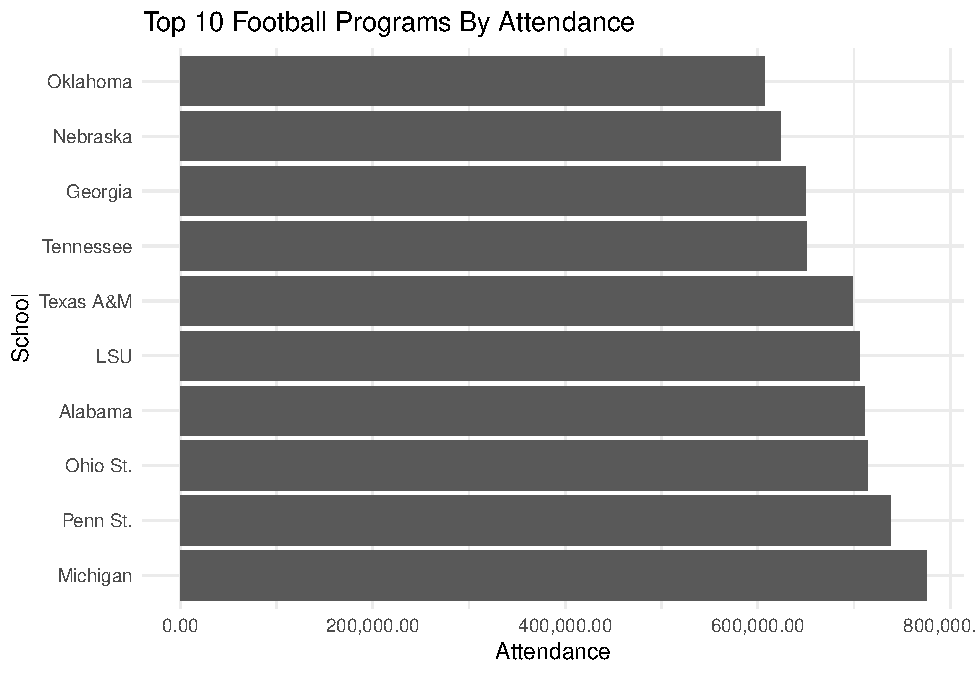
\includegraphics{SportsData_files/figure-latex/unnamed-chunk-116-1.pdf}

\chapter{Stacked bar charts}\label{stacked-bar-charts}

One of the elements of data visualization excellence, accoring to Tufte,
is inviting comparison. Often that comes in showing what proportion a
thing is in relation to the whole thing. With bar charts, if we have
information about the parts of the whole, we can stack them on top of
each other to compare them. And it's a simple change to what we've
already done.

\begin{Shaded}
\begin{Highlighting}[]
\KeywordTok{library}\NormalTok{(tidyverse)}
\end{Highlighting}
\end{Shaded}

We're going to use a dataset of graduation rates by gender by school in
the NCAA.
\href{https://unl.box.com/s/3nw1eokvs9zfdjyzvjaj3xdq01rm8sym}{You can
get it here}.

\begin{Shaded}
\begin{Highlighting}[]
\NormalTok{grads <-}\StringTok{ }\KeywordTok{read_csv}\NormalTok{(}\StringTok{'data/grads.csv'}\NormalTok{)}
\end{Highlighting}
\end{Shaded}

\begin{verbatim}
## Parsed with column specification:
## cols(
##   `Institution name` = col_character(),
##   `Primary Conference in Actual Year` = col_character(),
##   `Cohort year` = col_double(),
##   Gender = col_character(),
##   `Number of completers` = col_double(),
##   Total = col_double()
## )
\end{verbatim}

What we have here is the name of the school, the conference, the cohort
of when they started school, the gender, the number of that gender that
graduated and the total number of graduates in that cohort.

Let's pretend for a moment we're looking at the graduation rates of men
and women in the Big 10 Conference and we want to chart that. First,
let's work on our data. We need to filter the ``Big Ten Conference''
school, and we want the latest year, which is 2009. So we'll create a
dataframe called \texttt{BIG09} and populate it.

\begin{Shaded}
\begin{Highlighting}[]
\NormalTok{BIG09 <-}\StringTok{ }\NormalTok{grads }\OperatorTok\StringTok{ }\KeywordTok{filter}\NormalTok{(}\StringTok{`}\DataTypeTok{Primary Conference in Actual Year}\StringTok{`}\OperatorTok{==}\StringTok{"Big Ten Conference"}\NormalTok{) }\OperatorTok\StringTok{ }\KeywordTok{filter}\NormalTok{(}\StringTok{`}\DataTypeTok{Cohort year}\StringTok{`} \OperatorTok{==}\StringTok{ }\DecValTok{2009}\NormalTok{)}
\end{Highlighting}
\end{Shaded}

\begin{Shaded}
\begin{Highlighting}[]
\KeywordTok{head}\NormalTok{(BIG09)}
\end{Highlighting}
\end{Shaded}

\begin{verbatim}
## # A tibble: 6 x 6
##   `Institution na~ `Primary Confer~ `Cohort year` Gender `Number of comp~
##   <chr>            <chr>                    <dbl> <chr>             <dbl>
## 1 University of I~ Big Ten Confere~          2009 Men                2973
## 2 University of I~ Big Ten Confere~          2009 Women              2967
## 3 Northwestern Un~ Big Ten Confere~          2009 Men                 963
## 4 Northwestern Un~ Big Ten Confere~          2009 Women              1011
## 5 Indiana Univers~ Big Ten Confere~          2009 Men                2667
## 6 Indiana Univers~ Big Ten Confere~          2009 Women              2959
## # ... with 1 more variable: Total <dbl>
\end{verbatim}

Building on what we learned in the last chapter, we know we can turn
this into a bar chart with an x value, a weight and a geom\_bar. What're
going to add is a \texttt{fill}. The \texttt{fill} will stack bars on
each other based on which element it is. In this case, we can fill the
bar by Gender, which means it will stack the number of male graduates on
top of the number of female graduates and we can see how they compare.

\begin{Shaded}
\begin{Highlighting}[]
\KeywordTok{ggplot}\NormalTok{(BIG09, }\KeywordTok{aes}\NormalTok{(}\DataTypeTok{x=}\KeywordTok{reorder}\NormalTok{(}\StringTok{`}\DataTypeTok{Institution name}\StringTok{`}\NormalTok{, }\OperatorTok{-}\NormalTok{Total), }\DataTypeTok{weight=}\StringTok{`}\DataTypeTok{Number of completers}\StringTok{`}\NormalTok{, }\DataTypeTok{fill=}\NormalTok{Gender)) }\OperatorTok{+}\StringTok{ }\KeywordTok{geom_bar}\NormalTok{() }\OperatorTok{+}\StringTok{ }\KeywordTok{coord_flip}\NormalTok{()}
\end{Highlighting}
\end{Shaded}

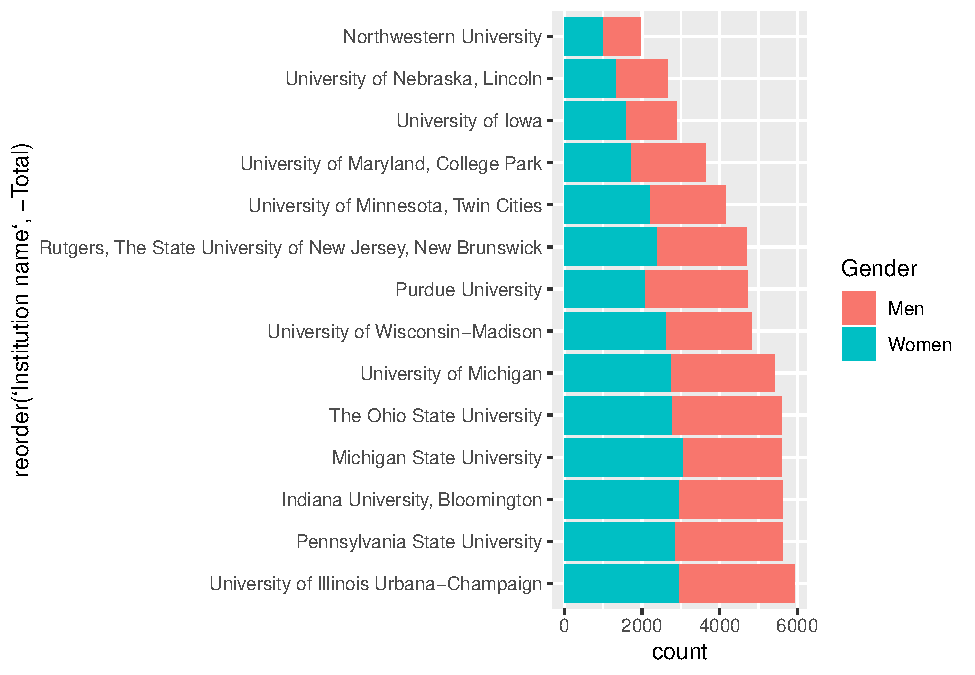
\includegraphics{SportsData_files/figure-latex/unnamed-chunk-121-1.pdf}

What's the problem with this chart?

Let me ask a different question -- which schools have larger differences
in male and female graduation rates? Can you compare Illnois to
Northwestern? Not really. We've charted the total numbers. We need the
percentage of the whole.

\begin{quote}
\textbf{YOUR TURN}: Using what you know -- hint: mutate -- how could you
chart this using percents of the whole instead of counts?
\end{quote}

\chapter{Waffle charts}\label{waffle-charts}

Pie charts are the devil. They should be an instant F in any data
visualization class. I'll give you an example of why.

What's the racial breakdown of journalism majors at UNL?

Here it is in a pie chart:

\begin{Shaded}
\begin{Highlighting}[]
\KeywordTok{library}\NormalTok{(tidyverse)}

\NormalTok{enrollment <-}\StringTok{ }\KeywordTok{read.csv}\NormalTok{(}\StringTok{"~/Dropbox/JOUR407-Data-Visualization/Data/collegeenrollment.csv"}\NormalTok{)}

\NormalTok{jour <-}\StringTok{ }\KeywordTok{filter}\NormalTok{(enrollment, MajorName }\OperatorTok{==}\StringTok{ "Journalism"}\NormalTok{)}

\NormalTok{jdf <-}\StringTok{ }\NormalTok{jour }\OperatorTok\StringTok{ }
\KeywordTok{group_by}\NormalTok{(Race) }\OperatorTok
\KeywordTok{summarise}\NormalTok{(}
       \DataTypeTok{total=}\KeywordTok{sum}\NormalTok{(Count)) }\OperatorTok
\KeywordTok{select}\NormalTok{(Race, total) }\OperatorTok\StringTok{ }
\KeywordTok{filter}\NormalTok{(total }\OperatorTok{!=}\StringTok{ }\DecValTok{0}\NormalTok{)}

\KeywordTok{ggplot}\NormalTok{(jdf, }\KeywordTok{aes}\NormalTok{(}\DataTypeTok{x=}\StringTok{""}\NormalTok{, }\DataTypeTok{y=}\NormalTok{total, }\DataTypeTok{fill=}\NormalTok{Race)) }\OperatorTok{+}\StringTok{ }\KeywordTok{geom_bar}\NormalTok{(}\DataTypeTok{width =} \DecValTok{1}\NormalTok{, }\DataTypeTok{stat =} \StringTok{"identity"}\NormalTok{) }\OperatorTok{+}\StringTok{ }\KeywordTok{coord_polar}\NormalTok{(}\StringTok{"y"}\NormalTok{, }\DataTypeTok{start=}\DecValTok{0}\NormalTok{)}
\end{Highlighting}
\end{Shaded}

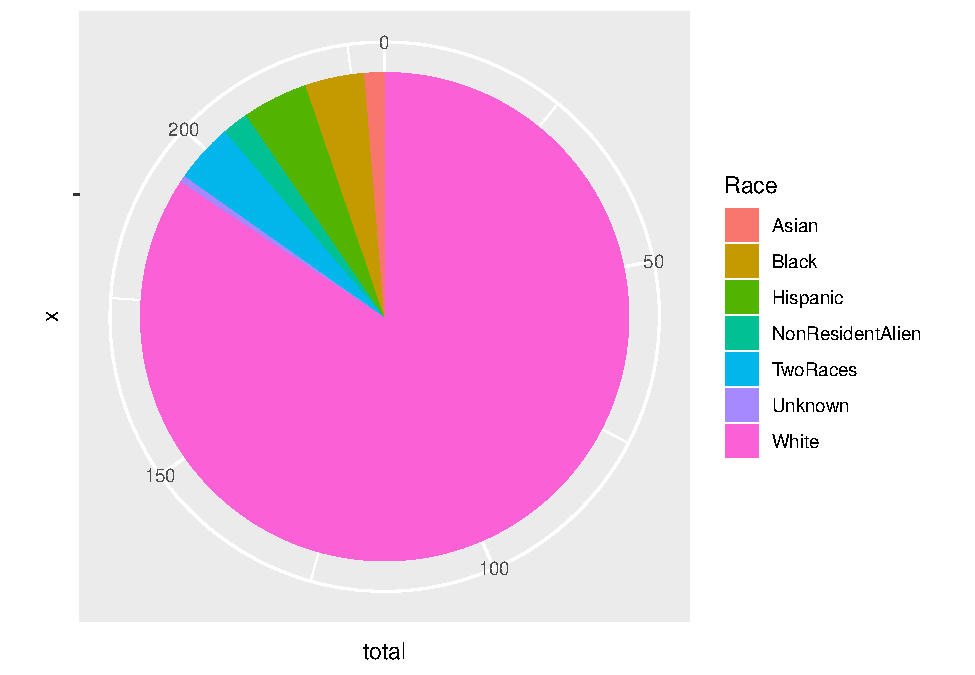
\includegraphics{SportsData_files/figure-latex/unnamed-chunk-122-1.pdf}
You can see, it's pretty white. But \ldots{} what about beyond that? How
carefully can you evaluate angles and area?

Not well.

So let's introduce a better way: The Waffle Chart. Some call it a square
pie chart. I personally hate that. Waffles it is.

First, install the library in the console:

\texttt{install.packages(\textquotesingle{}waffle\textquotesingle{})}

Now load it:

\begin{Shaded}
\begin{Highlighting}[]
\KeywordTok{library}\NormalTok{(waffle)}
\end{Highlighting}
\end{Shaded}

Let's look at the debacle in Ann Arbor with Nebraska basketball.
\href{https://www.sports-reference.com/cbb/boxscores/2019-02-28-19-michigan.html}{Here's
the box score}, which we'll use for this walkthrough.

The easiest way to do waffle charts is to make vectors of your data and
plug them in. To make a vector, we use the \texttt{c} or concatenate
function, something we've done before.

So let's look at \ldots{} shooting. We shot like crap that night, they
didn't.

\begin{Shaded}
\begin{Highlighting}[]
\NormalTok{nu <-}\StringTok{ }\KeywordTok{c}\NormalTok{(}\StringTok{"Made"}\NormalTok{=}\DecValTok{23}\NormalTok{, }\StringTok{"Missed"}\NormalTok{=}\DecValTok{44}\NormalTok{)}
\NormalTok{mi <-}\StringTok{ }\KeywordTok{c}\NormalTok{(}\StringTok{"Made"}\NormalTok{=}\DecValTok{30}\NormalTok{, }\StringTok{"Missed"}\NormalTok{=}\DecValTok{24}\NormalTok{)}
\end{Highlighting}
\end{Shaded}

So what does the breakdown of the night look like?

The waffle library can break this down in a way that's easier on the
eyes than a pie chart. We call the library, add the data, specify the
number of rows, give it a title and an x value label, and to clean up a
quirk of the library, we've got to specify colors.

\begin{Shaded}
\begin{Highlighting}[]
\KeywordTok{waffle}\NormalTok{(nu, }\DataTypeTok{rows =} \DecValTok{5}\NormalTok{, }\DataTypeTok{title=}\StringTok{"Nebraska's shooting night"}\NormalTok{, }\DataTypeTok{xlab=}\StringTok{"1 square = 1 shot"}\NormalTok{, }\DataTypeTok{colors =} \KeywordTok{c}\NormalTok{(}\StringTok{"black"}\NormalTok{, }\StringTok{"red"}\NormalTok{))}
\end{Highlighting}
\end{Shaded}

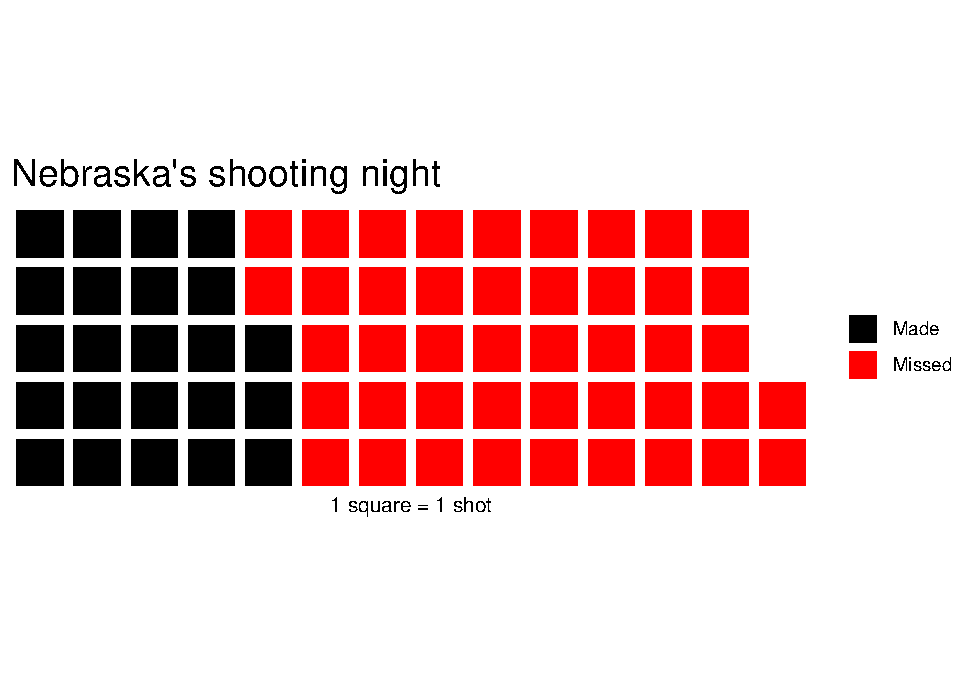
\includegraphics{SportsData_files/figure-latex/unnamed-chunk-125-1.pdf}

Or, we could make this two teams in the same chart.

\begin{Shaded}
\begin{Highlighting}[]
\NormalTok{game <-}\StringTok{ }\KeywordTok{c}\NormalTok{(}\StringTok{"Nebraska"}\NormalTok{=}\DecValTok{23}\NormalTok{, }\StringTok{"Michigan"}\NormalTok{=}\DecValTok{30}\NormalTok{)}
\end{Highlighting}
\end{Shaded}

\begin{Shaded}
\begin{Highlighting}[]
\KeywordTok{waffle}\NormalTok{(game, }\DataTypeTok{rows =} \DecValTok{5}\NormalTok{, }\DataTypeTok{title=}\StringTok{"Nebraska vs Michigan: made shots"}\NormalTok{, }\DataTypeTok{xlab=}\StringTok{"1 square = 1 shot"}\NormalTok{, }\DataTypeTok{colors =} \KeywordTok{c}\NormalTok{(}\StringTok{"red"}\NormalTok{, }\StringTok{"dark blue"}\NormalTok{))}
\end{Highlighting}
\end{Shaded}

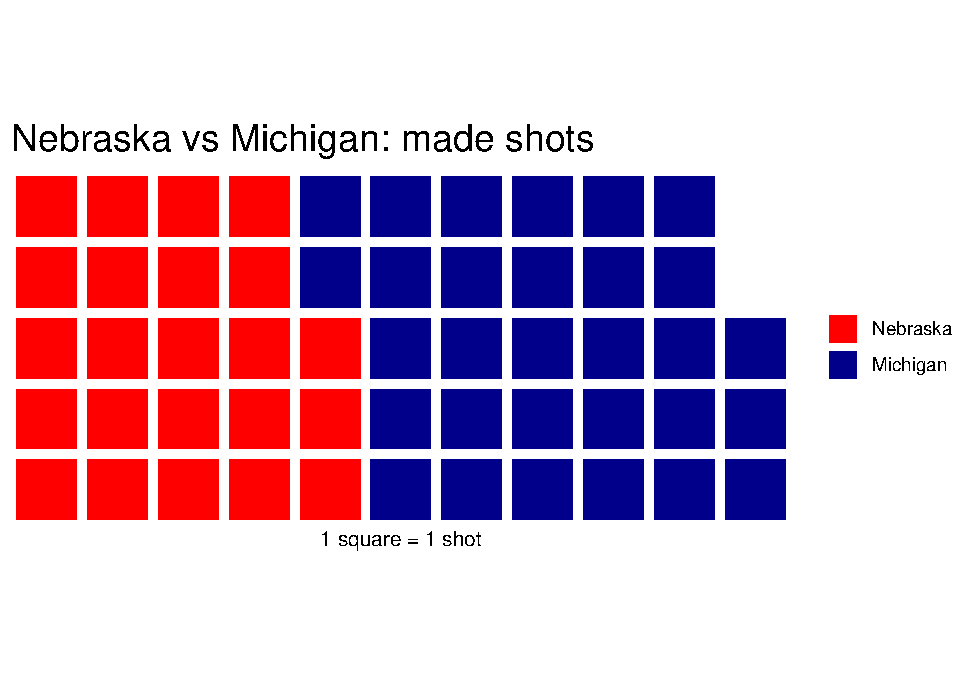
\includegraphics{SportsData_files/figure-latex/unnamed-chunk-127-1.pdf}

\section{Waffle Irons}\label{waffle-irons}

So what does it look like if we compare the two teams. Do do that -- and
I am not making this up -- you have to create a waffle iron. Get it?
Waffle charts? Iron?

\begin{Shaded}
\begin{Highlighting}[]
\KeywordTok{iron}\NormalTok{(}
 \KeywordTok{waffle}\NormalTok{(nu, }\DataTypeTok{rows =} \DecValTok{5}\NormalTok{, }\DataTypeTok{title=}\StringTok{"Nebraska's night shooting"}\NormalTok{, }\DataTypeTok{xlab=}\StringTok{"1 square = 1 shot"}\NormalTok{, }\DataTypeTok{colors =} \KeywordTok{c}\NormalTok{(}\StringTok{"black"}\NormalTok{, }\StringTok{"red"}\NormalTok{)),}
 \KeywordTok{waffle}\NormalTok{(mi, }\DataTypeTok{rows =} \DecValTok{5}\NormalTok{, }\DataTypeTok{title=}\StringTok{"Michigan's night shooting"}\NormalTok{, }\DataTypeTok{xlab=}\StringTok{"1 square = 1 shot"}\NormalTok{, }\DataTypeTok{colors =} \KeywordTok{c}\NormalTok{(}\StringTok{"dark blue"}\NormalTok{, }\StringTok{"yellow"}\NormalTok{))}
\NormalTok{)}
\end{Highlighting}
\end{Shaded}

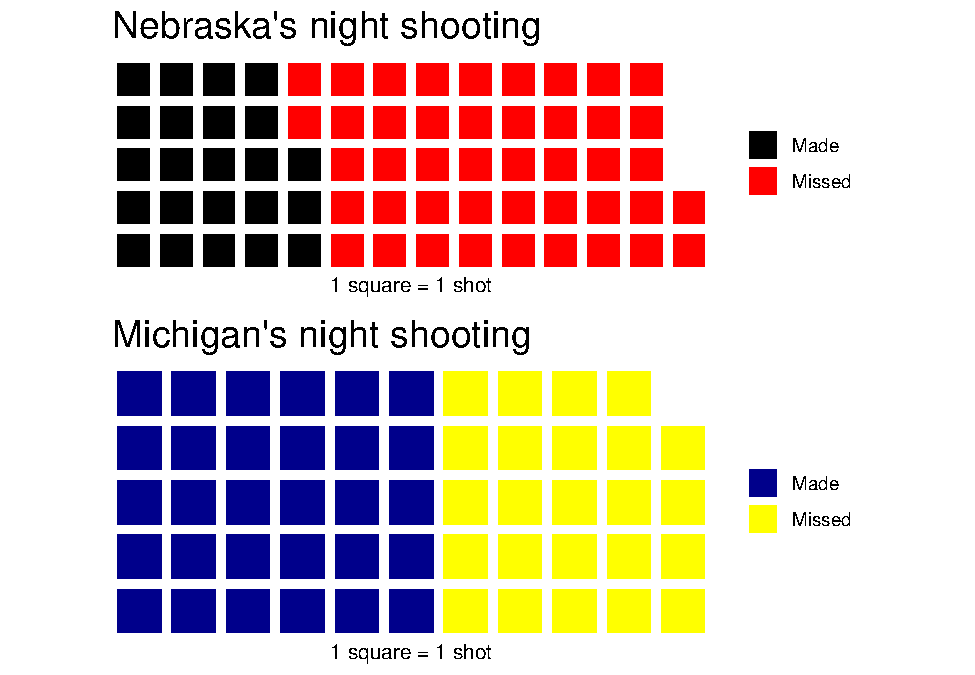
\includegraphics{SportsData_files/figure-latex/unnamed-chunk-128-1.pdf}

What do you notice about this chart? Notice how the squares aren't the
same size? Well, Michigan only took 54 shots. We took 67. So the squares
aren't the same size because the numbers aren't the same. We can fix
that by adding an unnamed padding number so the number of shots add up
to the same thing. Let's make the total for everyone be 70. So to do
that, we need to add a padding of 3 to Nebraska and a padding of 16 to
Michigan. REMEMBER: Don't name it or it'll show up in the legend.

\begin{Shaded}
\begin{Highlighting}[]
\NormalTok{nu <-}\StringTok{ }\KeywordTok{c}\NormalTok{(}\StringTok{"Made"}\NormalTok{=}\DecValTok{23}\NormalTok{, }\StringTok{"Missed"}\NormalTok{=}\DecValTok{44}\NormalTok{, }\DecValTok{3}\NormalTok{)}
\NormalTok{mi <-}\StringTok{ }\KeywordTok{c}\NormalTok{(}\StringTok{"Made"}\NormalTok{=}\DecValTok{30}\NormalTok{, }\StringTok{"Missed"}\NormalTok{=}\DecValTok{24}\NormalTok{, }\DecValTok{16}\NormalTok{)}
\end{Highlighting}
\end{Shaded}

Now, in our waffle iron, if we don't give that padding a color, we'll
get an error. So we need to make it white. Which, given our white
background, means it will disappear.

\begin{Shaded}
\begin{Highlighting}[]
\KeywordTok{iron}\NormalTok{(}
 \KeywordTok{waffle}\NormalTok{(nu, }\DataTypeTok{rows =} \DecValTok{5}\NormalTok{, }\DataTypeTok{title=}\StringTok{"Nebraska's night shooting"}\NormalTok{, }\DataTypeTok{colors =} \KeywordTok{c}\NormalTok{(}\StringTok{"black"}\NormalTok{, }\StringTok{"red"}\NormalTok{, }\StringTok{"white"}\NormalTok{)),}
 \KeywordTok{waffle}\NormalTok{(mi, }\DataTypeTok{rows =} \DecValTok{5}\NormalTok{, }\DataTypeTok{title=}\StringTok{"Michigan's night shooting"}\NormalTok{, }\DataTypeTok{xlab=}\StringTok{"1 square = 1 shot"}\NormalTok{, }\DataTypeTok{colors =} \KeywordTok{c}\NormalTok{(}\StringTok{"dark blue"}\NormalTok{, }\StringTok{"yellow"}\NormalTok{, }\StringTok{"white"}\NormalTok{))}
\NormalTok{)}
\end{Highlighting}
\end{Shaded}

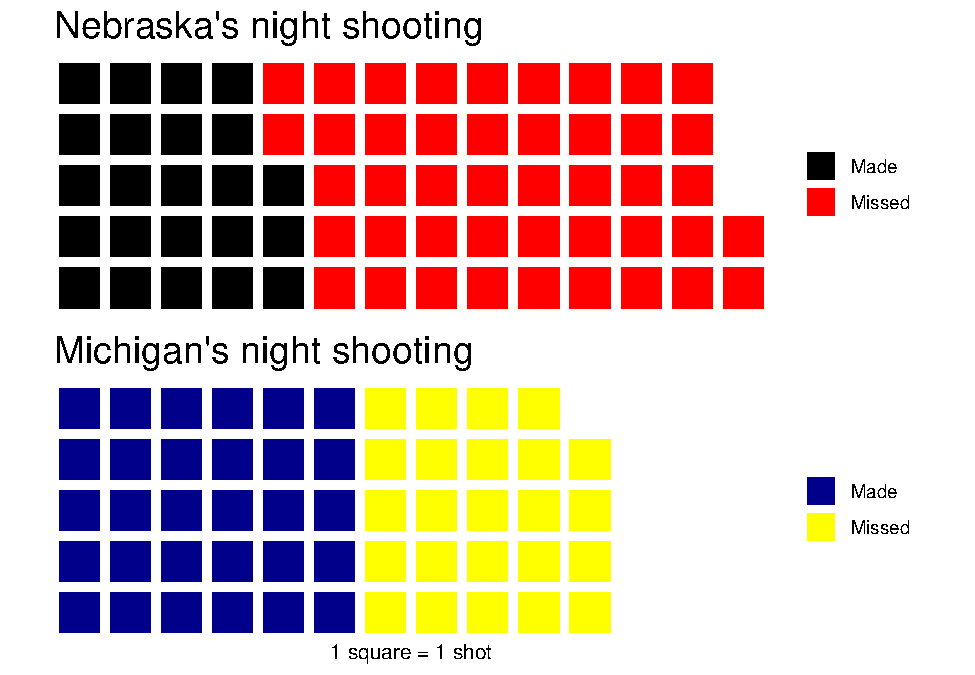
\includegraphics{SportsData_files/figure-latex/unnamed-chunk-130-1.pdf}

\chapter{Line charts}\label{line-charts}

Bar charts -- stacked or otherwise -- are good for showing relative size
of a thing compared to another thing. Line charts, which we work on
here, are good for showing change over time.

So let's look at how we can answer this question: Why was Nebraska
terrible last season?

Let's start getting all that we need. We can use the tidyverse shortcut.

\begin{Shaded}
\begin{Highlighting}[]
\KeywordTok{library}\NormalTok{(tidyverse)}
\end{Highlighting}
\end{Shaded}

Now we'll import the data you created. Mine looks like this:

\begin{Shaded}
\begin{Highlighting}[]
\NormalTok{logs <-}\StringTok{ }\KeywordTok{read_csv}\NormalTok{(}\StringTok{"data/logs19.csv"}\NormalTok{)}
\end{Highlighting}
\end{Shaded}

\begin{verbatim}
## Warning: Missing column names filled in: 'X1' [1]
\end{verbatim}

\begin{verbatim}
## Parsed with column specification:
## cols(
##   .default = col_double(),
##   Date = col_date(format = ""),
##   HomeAway = col_character(),
##   Opponent = col_character(),
##   W_L = col_character(),
##   Blank = col_logical(),
##   Team = col_character(),
##   Conference = col_character(),
##   season = col_character()
## )
\end{verbatim}

\begin{verbatim}
## See spec(...) for full column specifications.
\end{verbatim}

This data has every game from every team in it, so we need to use
filtering to limit it, because we just want to look at Nebraska. If you
don't remember, flip back to chapter 5.

\begin{Shaded}
\begin{Highlighting}[]
\NormalTok{nu <-}\StringTok{ }\NormalTok{logs }\OperatorTok\StringTok{ }\KeywordTok{filter}\NormalTok{(Team }\OperatorTok{==}\StringTok{ "Nebraska Cornhuskers"}\NormalTok{)}
\end{Highlighting}
\end{Shaded}

Because this data has just Nebraska data in it, the dates are formatted
correctly, and the data is long data (instead of wide), we have what we
need to make line charts.

Line charts, unlike bar charts, do have a y-axis. So in our ggplot step,
we have to define what our x and y axes are. In this case, the x axis is
our Date -- the most common x axis in line charts is going to be a date
of some variety -- and y in this case is up to us. We've seen from
previous walkthroughs that how well a team shoots the ball has a lot to
do with how well a team does in a season, so let's chart that.

\begin{Shaded}
\begin{Highlighting}[]
\KeywordTok{ggplot}\NormalTok{(nu, }\KeywordTok{aes}\NormalTok{(}\DataTypeTok{x=}\NormalTok{Date, }\DataTypeTok{y=}\NormalTok{TeamFGPCT)) }\OperatorTok{+}\StringTok{ }\KeywordTok{geom_line}\NormalTok{()}
\end{Highlighting}
\end{Shaded}

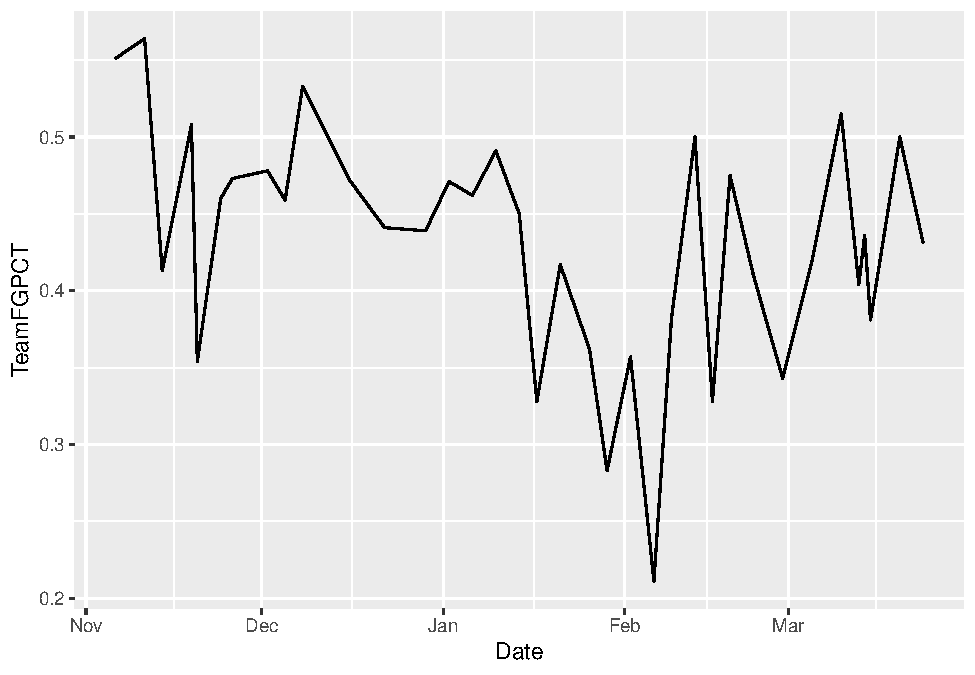
\includegraphics{SportsData_files/figure-latex/unnamed-chunk-134-1.pdf}

See a problem here? Note the Y axis doesn't start with zero. That makes
this look worse than it is (and that February swoon is pretty bad). To
make the axis what you want, you can use \texttt{scale\_x\_continuous}
or \texttt{scale\_y\_continuous} and pass in a list with the bottom and
top value you want. You do that like this:

\begin{Shaded}
\begin{Highlighting}[]
\KeywordTok{ggplot}\NormalTok{(nu, }\KeywordTok{aes}\NormalTok{(}\DataTypeTok{x=}\NormalTok{Date, }\DataTypeTok{y=}\NormalTok{TeamFGPCT)) }\OperatorTok{+}\StringTok{ }\KeywordTok{geom_line}\NormalTok{() }\OperatorTok{+}\StringTok{ }\KeywordTok{scale_y_continuous}\NormalTok{(}\DataTypeTok{limits =} \KeywordTok{c}\NormalTok{(}\DecValTok{0}\NormalTok{, .}\DecValTok{6}\NormalTok{))}
\end{Highlighting}
\end{Shaded}

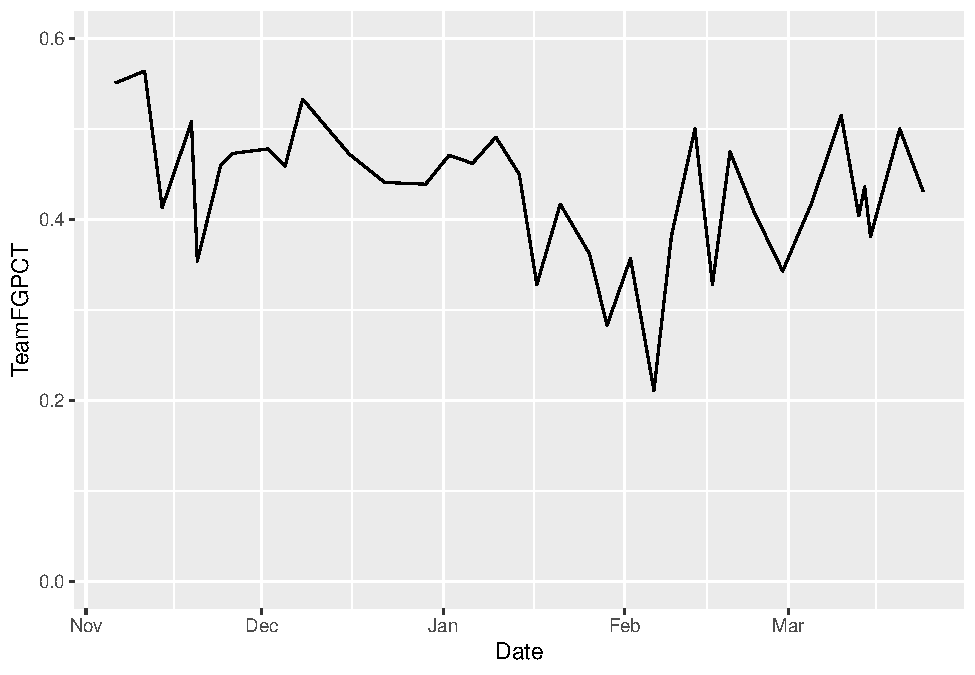
\includegraphics{SportsData_files/figure-latex/unnamed-chunk-135-1.pdf}

Note also that our X axis labels are automated. It knows it's a date and
it just labels it by month. \#\# This is too simple.

With datasets, we want to invite comparison. So let's answer the
question visually. Let's put two lines on the same chart. How does
Nebraska compare to Michigan State and Purdue, the eventual regular
season co-champions?

\begin{Shaded}
\begin{Highlighting}[]
\NormalTok{msu <-}\StringTok{ }\NormalTok{logs }\OperatorTok\StringTok{ }\KeywordTok{filter}\NormalTok{(Team }\OperatorTok{==}\StringTok{ "Michigan State Spartans"}\NormalTok{)}
\end{Highlighting}
\end{Shaded}

In this case, because we have two different datasets, we're going to put
everything in the geom instead of the ggplot step. We also have to
explicitly state what dataset we're using by saying \texttt{data=} in
the geom step.

First, let's chart Nebraska. Read carefully. First we set the data. Then
we set our aesthetic. Unlike bars, we need an X and a Y variable. In
this case, our X is the date of the game, Y is the thing we want the
lines to move with. In this case, the Team Field Goal Percentage --
TeamFGPCT.

\begin{Shaded}
\begin{Highlighting}[]
\KeywordTok{ggplot}\NormalTok{() }\OperatorTok{+}\StringTok{ }\KeywordTok{geom_line}\NormalTok{(}\DataTypeTok{data=}\NormalTok{nu, }\KeywordTok{aes}\NormalTok{(}\DataTypeTok{x=}\NormalTok{Date, }\DataTypeTok{y=}\NormalTok{TeamFGPCT), }\DataTypeTok{color=}\StringTok{"red"}\NormalTok{)}
\end{Highlighting}
\end{Shaded}

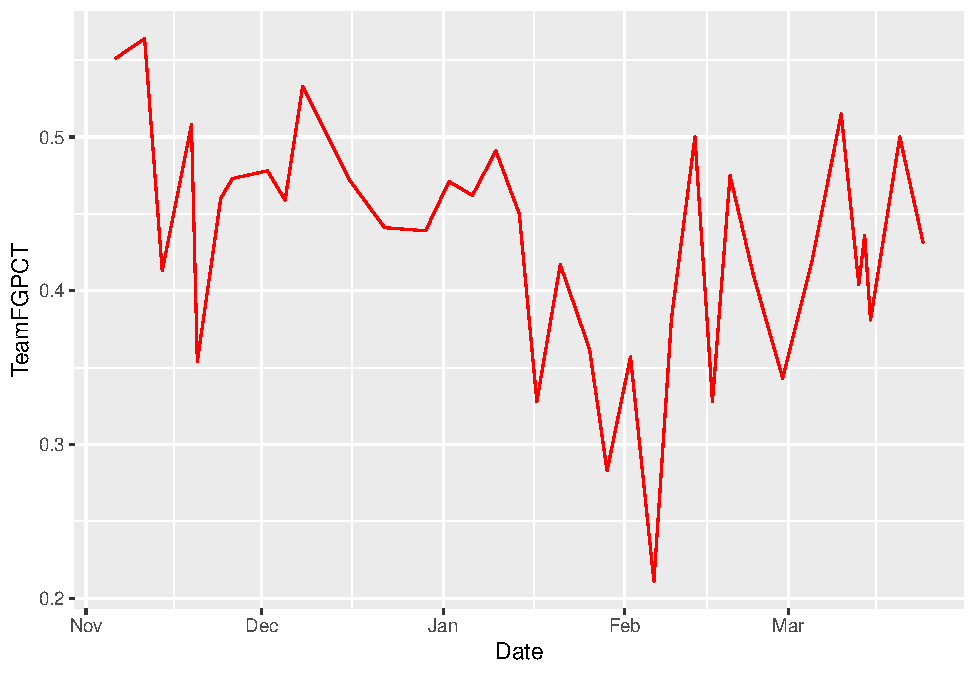
\includegraphics{SportsData_files/figure-latex/unnamed-chunk-137-1.pdf}

Now, by using +, we can add Michigan State to it. REMEMBER COPY AND
PASTE IS A THING. Nothing changes except what data you are using.

\begin{Shaded}
\begin{Highlighting}[]
\KeywordTok{ggplot}\NormalTok{() }\OperatorTok{+}\StringTok{ }\KeywordTok{geom_line}\NormalTok{(}\DataTypeTok{data=}\NormalTok{nu, }\KeywordTok{aes}\NormalTok{(}\DataTypeTok{x=}\NormalTok{Date, }\DataTypeTok{y=}\NormalTok{TeamFGPCT), }\DataTypeTok{color=}\StringTok{"red"}\NormalTok{) }\OperatorTok{+}\StringTok{ }\KeywordTok{geom_line}\NormalTok{(}\DataTypeTok{data=}\NormalTok{msu, }\KeywordTok{aes}\NormalTok{(}\DataTypeTok{x=}\NormalTok{Date, }\DataTypeTok{y=}\NormalTok{TeamFGPCT), }\DataTypeTok{color=}\StringTok{"dark green"}\NormalTok{)}
\end{Highlighting}
\end{Shaded}

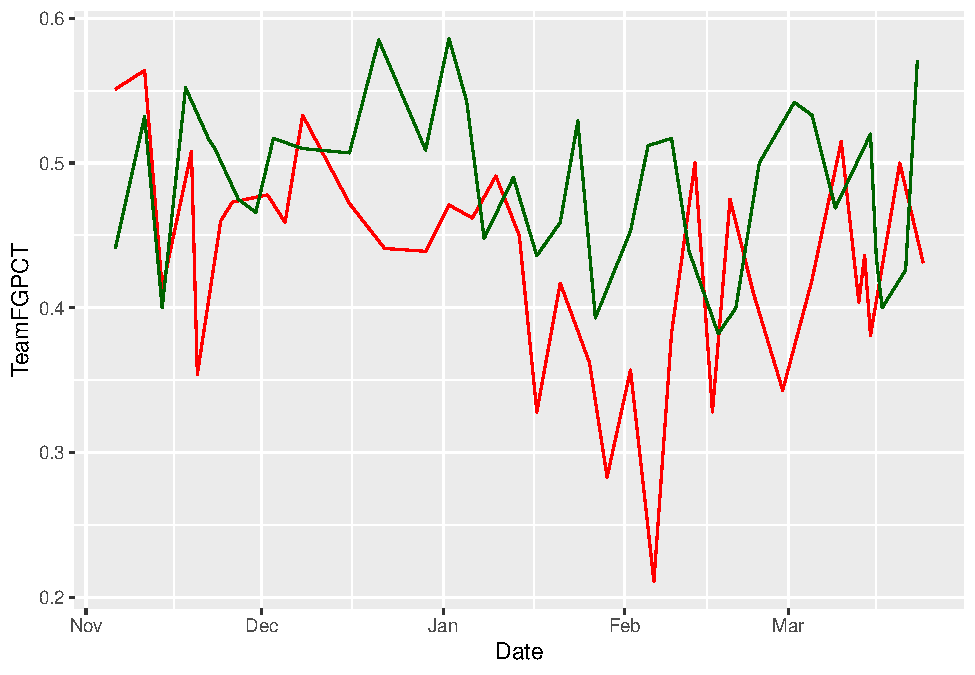
\includegraphics{SportsData_files/figure-latex/unnamed-chunk-138-1.pdf}

Let's flatten our lines out by zeroing the Y axis.

\begin{Shaded}
\begin{Highlighting}[]
\KeywordTok{ggplot}\NormalTok{() }\OperatorTok{+}\StringTok{ }\KeywordTok{geom_line}\NormalTok{(}\DataTypeTok{data=}\NormalTok{nu, }\KeywordTok{aes}\NormalTok{(}\DataTypeTok{x=}\NormalTok{Date, }\DataTypeTok{y=}\NormalTok{TeamFGPCT), }\DataTypeTok{color=}\StringTok{"red"}\NormalTok{) }\OperatorTok{+}\StringTok{ }\KeywordTok{geom_line}\NormalTok{(}\DataTypeTok{data=}\NormalTok{msu, }\KeywordTok{aes}\NormalTok{(}\DataTypeTok{x=}\NormalTok{Date, }\DataTypeTok{y=}\NormalTok{TeamFGPCT), }\DataTypeTok{color=}\StringTok{"dark green"}\NormalTok{) }\OperatorTok{+}\StringTok{ }\KeywordTok{scale_y_continuous}\NormalTok{(}\DataTypeTok{limits =} \KeywordTok{c}\NormalTok{(}\DecValTok{0}\NormalTok{, .}\DecValTok{6}\NormalTok{))}
\end{Highlighting}
\end{Shaded}

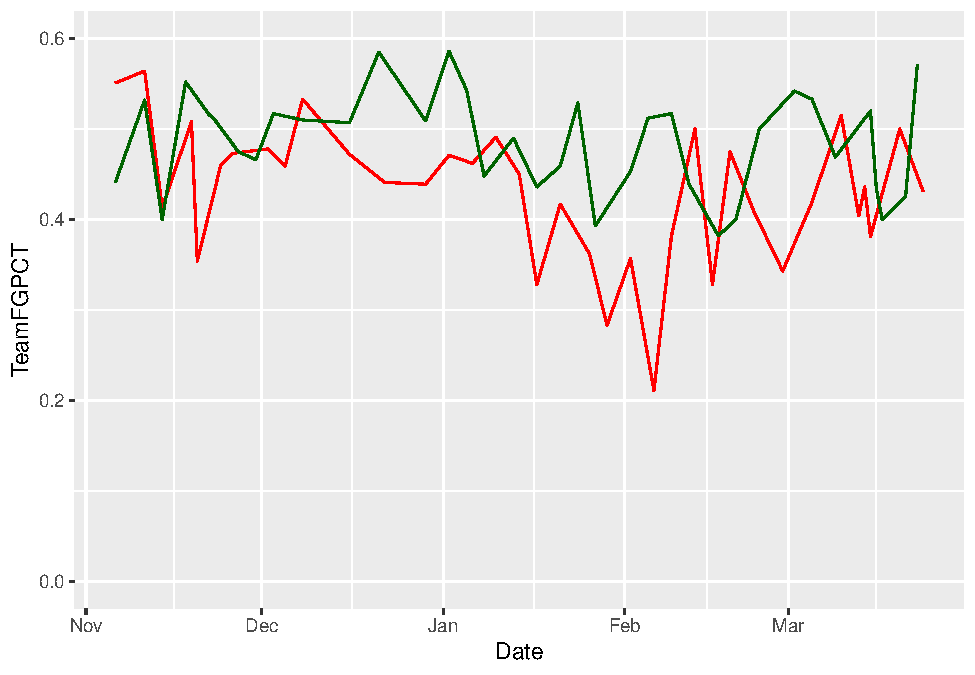
\includegraphics{SportsData_files/figure-latex/unnamed-chunk-139-1.pdf}

So visually speaking, the difference between Nebraska and Michigan
State's season is that Michigan State stayed mostly on an even keel, and
Nebraska went on a two month swoon.

\section{But what if I wanted to add a lot of
lines.}\label{but-what-if-i-wanted-to-add-a-lot-of-lines.}

Fine. How about all Power Five Schools? This data for example purposes.
You don't have to do it.

\begin{Shaded}
\begin{Highlighting}[]
\NormalTok{powerfive <-}\StringTok{ }\KeywordTok{c}\NormalTok{(}\StringTok{"SEC"}\NormalTok{, }\StringTok{"Big Ten"}\NormalTok{, }\StringTok{"Pac-12"}\NormalTok{, }\StringTok{"Big 12"}\NormalTok{, }\StringTok{"ACC"}\NormalTok{)}

\NormalTok{p5conf <-}\StringTok{ }\NormalTok{logs }\OperatorTok\StringTok{ }\KeywordTok{filter}\NormalTok{(Conference }\OperatorTok\StringTok{ }\NormalTok{powerfive)}
\end{Highlighting}
\end{Shaded}

I can keep layering on layers all day if I want. And if my dataset has
more than one team in it, I need to use the \texttt{group} command. And,
the layering comes in order -- so if you're going to layer a bunch of
lines with a smaller group of lines, you want the bunch on the bottom.
So to do that, your code stacks from the bottom. The first geom in the
code gets rendered first. The second gets layered on top of that. The
third gets layered on that and so on.

\begin{Shaded}
\begin{Highlighting}[]
\KeywordTok{ggplot}\NormalTok{() }\OperatorTok{+}\StringTok{ }\KeywordTok{geom_line}\NormalTok{(}\DataTypeTok{data=}\NormalTok{p5conf, }\KeywordTok{aes}\NormalTok{(}\DataTypeTok{x=}\NormalTok{Date, }\DataTypeTok{y=}\NormalTok{TeamFGPCT, }\DataTypeTok{group=}\NormalTok{Team), }\DataTypeTok{color=}\StringTok{"light grey"}\NormalTok{) }\OperatorTok{+}\StringTok{ }\KeywordTok{geom_line}\NormalTok{(}\DataTypeTok{data=}\NormalTok{nu, }\KeywordTok{aes}\NormalTok{(}\DataTypeTok{x=}\NormalTok{Date, }\DataTypeTok{y=}\NormalTok{TeamFGPCT), }\DataTypeTok{color=}\StringTok{"red"}\NormalTok{) }\OperatorTok{+}\StringTok{ }\KeywordTok{geom_line}\NormalTok{(}\DataTypeTok{data=}\NormalTok{msu, }\KeywordTok{aes}\NormalTok{(}\DataTypeTok{x=}\NormalTok{Date, }\DataTypeTok{y=}\NormalTok{TeamFGPCT), }\DataTypeTok{color=}\StringTok{"dark green"}\NormalTok{) }\OperatorTok{+}\StringTok{ }\KeywordTok{scale_y_continuous}\NormalTok{(}\DataTypeTok{limits =} \KeywordTok{c}\NormalTok{(}\DecValTok{0}\NormalTok{, .}\DecValTok{6}\NormalTok{))}
\end{Highlighting}
\end{Shaded}

\begin{verbatim}
## Warning: Removed 1 rows containing missing values (geom_path).
\end{verbatim}

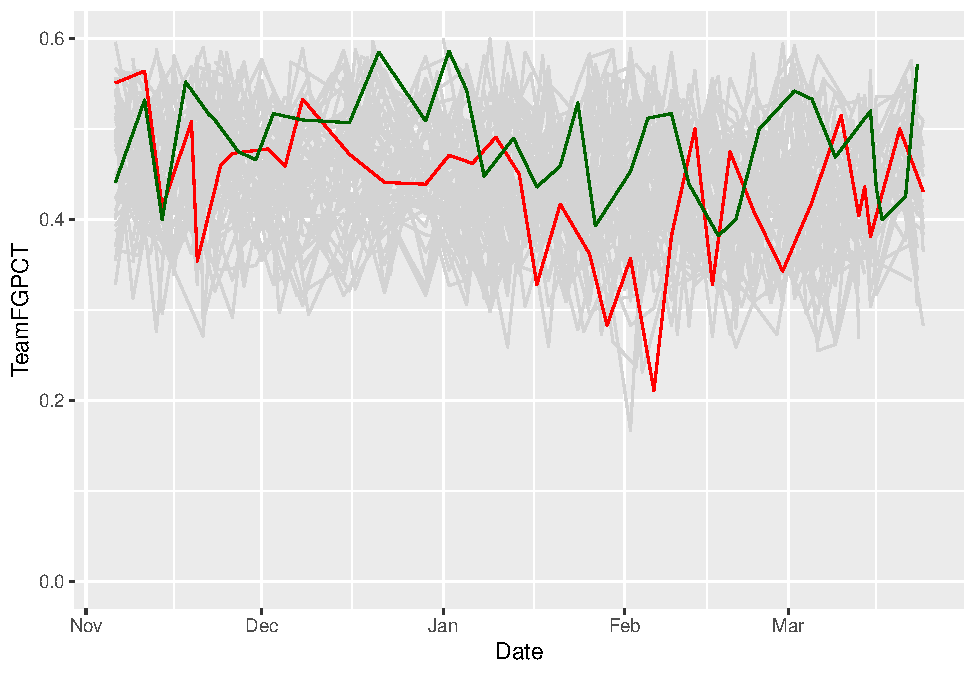
\includegraphics{SportsData_files/figure-latex/unnamed-chunk-141-1.pdf}

What do we see here? How has Nebraska and Michigan State's season
evolved against all the rest of the teams in college basketball?

But how does that compare to the average? We can add that pretty easily
by creating a new dataframe with it and add another geom\_line.

\begin{Shaded}
\begin{Highlighting}[]
\NormalTok{average <-}\StringTok{ }\NormalTok{logs }\OperatorTok\StringTok{ }\KeywordTok{group_by}\NormalTok{(Date) }\OperatorTok\StringTok{ }\KeywordTok{summarise}\NormalTok{(}\DataTypeTok{mean_shooting=}\KeywordTok{mean}\NormalTok{(TeamFGPCT))}
\end{Highlighting}
\end{Shaded}

\begin{Shaded}
\begin{Highlighting}[]
\KeywordTok{ggplot}\NormalTok{() }\OperatorTok{+}\StringTok{ }\KeywordTok{geom_line}\NormalTok{(}\DataTypeTok{data=}\NormalTok{p5conf, }\KeywordTok{aes}\NormalTok{(}\DataTypeTok{x=}\NormalTok{Date, }\DataTypeTok{y=}\NormalTok{TeamFGPCT, }\DataTypeTok{group=}\NormalTok{Team), }\DataTypeTok{color=}\StringTok{"light grey"}\NormalTok{) }\OperatorTok{+}\StringTok{ }\KeywordTok{geom_line}\NormalTok{(}\DataTypeTok{data=}\NormalTok{nu, }\KeywordTok{aes}\NormalTok{(}\DataTypeTok{x=}\NormalTok{Date, }\DataTypeTok{y=}\NormalTok{TeamFGPCT), }\DataTypeTok{color=}\StringTok{"red"}\NormalTok{) }\OperatorTok{+}\StringTok{ }\KeywordTok{geom_line}\NormalTok{(}\DataTypeTok{data=}\NormalTok{msu, }\KeywordTok{aes}\NormalTok{(}\DataTypeTok{x=}\NormalTok{Date, }\DataTypeTok{y=}\NormalTok{TeamFGPCT), }\DataTypeTok{color=}\StringTok{"dark green"}\NormalTok{) }\OperatorTok{+}\StringTok{ }\KeywordTok{geom_line}\NormalTok{(}\DataTypeTok{data=}\NormalTok{average, }\KeywordTok{aes}\NormalTok{(}\DataTypeTok{x=}\NormalTok{Date, }\DataTypeTok{y=}\NormalTok{mean_shooting), }\DataTypeTok{color=}\StringTok{"black"}\NormalTok{) }\OperatorTok{+}\StringTok{ }\KeywordTok{scale_y_continuous}\NormalTok{(}\DataTypeTok{limits =} \KeywordTok{c}\NormalTok{(}\DecValTok{0}\NormalTok{, .}\DecValTok{6}\NormalTok{))}
\end{Highlighting}
\end{Shaded}

\begin{verbatim}
## Warning: Removed 1 rows containing missing values (geom_path).
\end{verbatim}

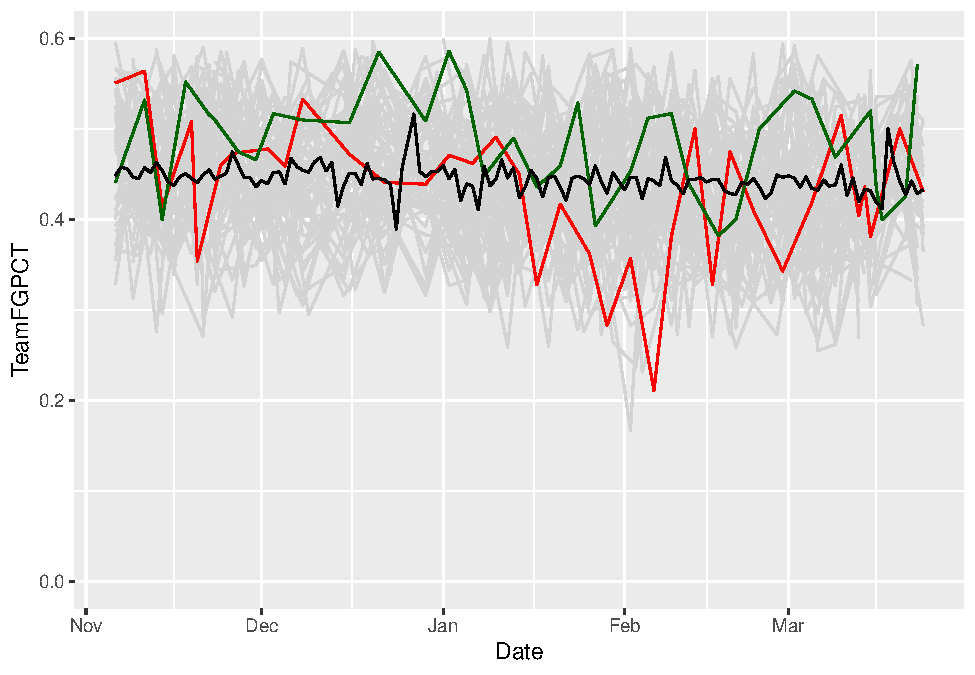
\includegraphics{SportsData_files/figure-latex/unnamed-chunk-143-1.pdf}

\chapter{Step charts}\label{step-charts}

Step charts are a method of showing progress toward something. There's
been two great examples lately. First is the Washignton Post looking at
\href{https://www.washingtonpost.com/graphics/sports/lebron-james-michael-jordan-nba-scoring-list/?utm_term=.481074150849}{Lebron
passing Jordan's career point total}. Another is John Burn-Murdoch's
work at the Financial Times (which is paywalled) about soccer stars.
\href{http://johnburnmurdoch.github.io/projects/goal-lines/CL/}{Here's
an example of his work outside the paywall}.

To replicate this, we need cumulative data -- data that is the running
total of data at a given point. So think of it this way -- Nebraska
scores 50 points in a basketball game and then 50 more the next, their
cumulative total at two games is 100 points.

Step charts can be used for all kinds of things -- showing how a
player's career has evolved over time, how a team fares over a season,
or franchise history. Let's walk through an example.

\begin{Shaded}
\begin{Highlighting}[]
\KeywordTok{library}\NormalTok{(tidyverse)}
\end{Highlighting}
\end{Shaded}

And we'll use our basketball log data.

\begin{Shaded}
\begin{Highlighting}[]
\NormalTok{logs <-}\StringTok{ }\KeywordTok{read_csv}\NormalTok{(}\StringTok{"data/logs19.csv"}\NormalTok{)}
\end{Highlighting}
\end{Shaded}

\begin{verbatim}
## Warning: Missing column names filled in: 'X1' [1]
\end{verbatim}

\begin{verbatim}
## Parsed with column specification:
## cols(
##   .default = col_double(),
##   Date = col_date(format = ""),
##   HomeAway = col_character(),
##   Opponent = col_character(),
##   W_L = col_character(),
##   Blank = col_logical(),
##   Team = col_character(),
##   Conference = col_character(),
##   season = col_character()
## )
\end{verbatim}

\begin{verbatim}
## See spec(...) for full column specifications.
\end{verbatim}

Here we're going to look at the scoring differential of teams. If you
score more than your opponent, you win. So it stands to reason that if
you score a lot more than your opponent over the course of a season, you
should be very good, right? Let's see.

The first thing we're going to do is calculate that differential. Then,
we'll group it by the team. After that, we're going to summarize using a
new function called \texttt{cumsum} or cumulative sum -- the sum for
each game as we go forward.

\begin{Shaded}
\begin{Highlighting}[]
\NormalTok{difflogs <-}\StringTok{ }\NormalTok{logs }\OperatorTok\StringTok{ }\KeywordTok{mutate}\NormalTok{(}\DataTypeTok{Differential =}\NormalTok{ TeamScore }\OperatorTok{-}\StringTok{ }\NormalTok{OpponentScore) }\OperatorTok\StringTok{ }\KeywordTok{group_by}\NormalTok{(Team) }\OperatorTok\StringTok{ }\KeywordTok{mutate}\NormalTok{(}\DataTypeTok{CumDiff =} \KeywordTok{cumsum}\NormalTok{(Differential))}
\end{Highlighting}
\end{Shaded}

Now that we have the cumulative sum for each, let's filter it down to
just Big Ten teams.

\begin{Shaded}
\begin{Highlighting}[]
\NormalTok{bigdiff <-}\StringTok{ }\NormalTok{difflogs }\OperatorTok\StringTok{ }\KeywordTok{filter}\NormalTok{(Conference }\OperatorTok{==}\StringTok{ "Big Ten"}\NormalTok{)}
\end{Highlighting}
\end{Shaded}

The step chart is it's own geom, so we can employ it just like we have
the others. It works almost exactly the same as a line chart, but it
just has to use the cumulative sum instead of a regular value.

\begin{Shaded}
\begin{Highlighting}[]
\KeywordTok{ggplot}\NormalTok{() }\OperatorTok{+}\StringTok{ }\KeywordTok{geom_step}\NormalTok{(}\DataTypeTok{data=}\NormalTok{bigdiff, }\KeywordTok{aes}\NormalTok{(}\DataTypeTok{x=}\NormalTok{Date, }\DataTypeTok{y=}\NormalTok{CumDiff, }\DataTypeTok{group=}\NormalTok{Team))}
\end{Highlighting}
\end{Shaded}

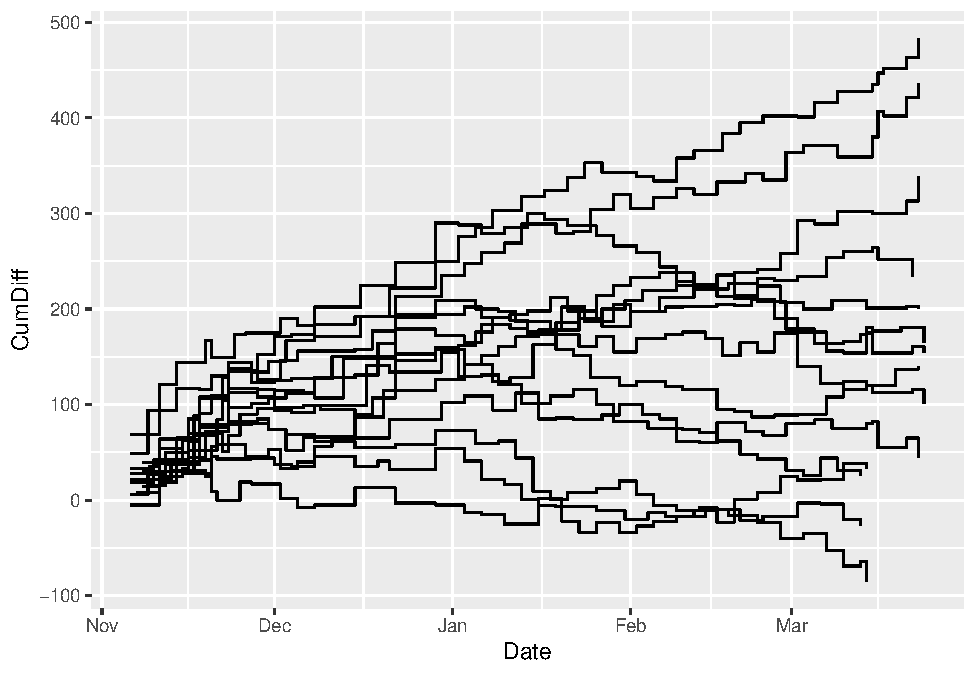
\includegraphics{SportsData_files/figure-latex/unnamed-chunk-148-1.pdf}

Let's try a different element of the aesthetic: color, but this time
inside the aesthetic. Last time, we did the color outside. When you put
it inside, you pass it a column name and ggplot will color each line
based on what thing that is, and it will create a legend that labels
each line that thing.

\begin{Shaded}
\begin{Highlighting}[]
\KeywordTok{ggplot}\NormalTok{() }\OperatorTok{+}\StringTok{ }\KeywordTok{geom_step}\NormalTok{(}\DataTypeTok{data=}\NormalTok{bigdiff, }\KeywordTok{aes}\NormalTok{(}\DataTypeTok{x=}\NormalTok{Date, }\DataTypeTok{y=}\NormalTok{CumDiff, }\DataTypeTok{group=}\NormalTok{Team, }\DataTypeTok{color=}\NormalTok{Team))}
\end{Highlighting}
\end{Shaded}

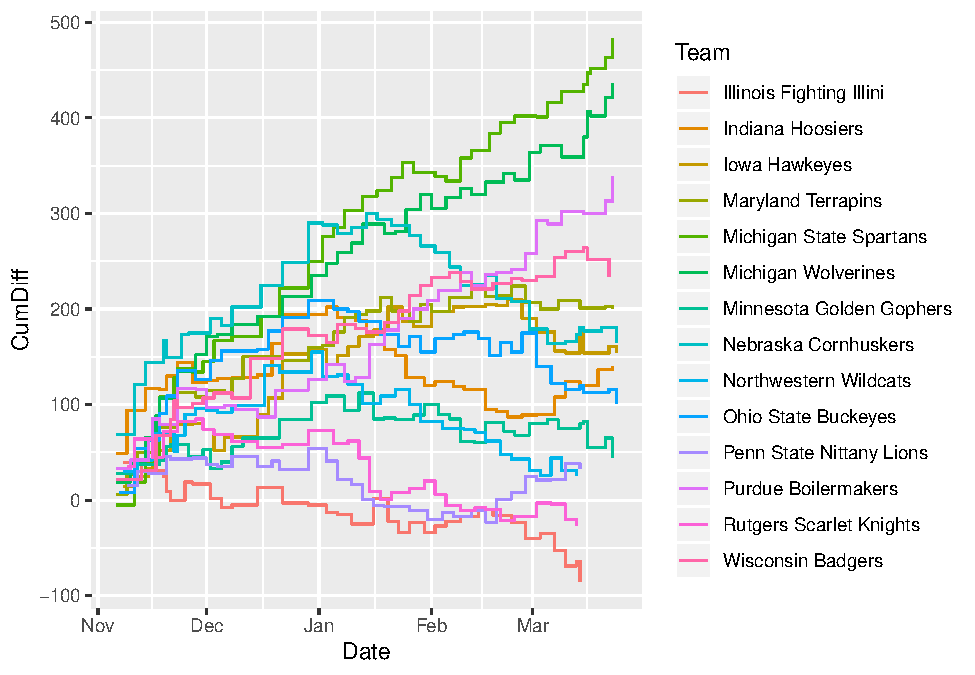
\includegraphics{SportsData_files/figure-latex/unnamed-chunk-149-1.pdf}

From this, we can see two teams in the Big Ten have negative point
differentials on the season -- Illinois and Rutgers.

Let's look at those top teams plus Nebraska.

\begin{Shaded}
\begin{Highlighting}[]
\NormalTok{nu <-}\StringTok{ }\NormalTok{bigdiff }\OperatorTok\StringTok{ }\KeywordTok{filter}\NormalTok{(Team }\OperatorTok{==}\StringTok{ "Nebraska Cornhuskers"}\NormalTok{)}
\NormalTok{mi <-}\StringTok{ }\NormalTok{bigdiff }\OperatorTok\StringTok{ }\KeywordTok{filter}\NormalTok{(Team }\OperatorTok{==}\StringTok{ "Michigan Wolverines"}\NormalTok{)}
\NormalTok{ms <-}\StringTok{ }\NormalTok{bigdiff }\OperatorTok\StringTok{ }\KeywordTok{filter}\NormalTok{(Team }\OperatorTok{==}\StringTok{ "Michigan State Spartans"}\NormalTok{)}
\end{Highlighting}
\end{Shaded}

Let's introduce a couple of new things here. First, note when I take the
color OUT of the aesthetic, the legend disappears.

The second thing I'm going to add is the annotation layer. In this case,
I am adding a text annotation layer, and I can specify where by adding
in a x and a y value where I want to put it. This takes some finesse.
After that, I'm going to add labels and a theme.

\begin{Shaded}
\begin{Highlighting}[]
\KeywordTok{ggplot}\NormalTok{() }\OperatorTok{+}\StringTok{ }
\StringTok{  }\KeywordTok{geom_step}\NormalTok{(}\DataTypeTok{data=}\NormalTok{bigdiff, }\KeywordTok{aes}\NormalTok{(}\DataTypeTok{x=}\NormalTok{Date, }\DataTypeTok{y=}\NormalTok{CumDiff, }\DataTypeTok{group=}\NormalTok{Team), }\DataTypeTok{color=}\StringTok{"light grey"}\NormalTok{) }\OperatorTok{+}
\StringTok{  }\KeywordTok{geom_step}\NormalTok{(}\DataTypeTok{data=}\NormalTok{nu, }\KeywordTok{aes}\NormalTok{(}\DataTypeTok{x=}\NormalTok{Date, }\DataTypeTok{y=}\NormalTok{CumDiff, }\DataTypeTok{group=}\NormalTok{Team), }\DataTypeTok{color=}\StringTok{"red"}\NormalTok{) }\OperatorTok{+}\StringTok{ }
\StringTok{  }\KeywordTok{geom_step}\NormalTok{(}\DataTypeTok{data=}\NormalTok{mi, }\KeywordTok{aes}\NormalTok{(}\DataTypeTok{x=}\NormalTok{Date, }\DataTypeTok{y=}\NormalTok{CumDiff, }\DataTypeTok{group=}\NormalTok{Team), }\DataTypeTok{color=}\StringTok{"blue"}\NormalTok{) }\OperatorTok{+}\StringTok{ }
\StringTok{  }\KeywordTok{geom_step}\NormalTok{(}\DataTypeTok{data=}\NormalTok{ms, }\KeywordTok{aes}\NormalTok{(}\DataTypeTok{x=}\NormalTok{Date, }\DataTypeTok{y=}\NormalTok{CumDiff, }\DataTypeTok{group=}\NormalTok{Team), }\DataTypeTok{color=}\StringTok{"dark green"}\NormalTok{) }\OperatorTok{+}
\StringTok{  }\KeywordTok{annotate}\NormalTok{(}\StringTok{"text"}\NormalTok{, }\DataTypeTok{x=}\NormalTok{(}\KeywordTok{as.Date}\NormalTok{(}\StringTok{"2018-12-10"}\NormalTok{)), }\DataTypeTok{y=}\DecValTok{220}\NormalTok{, }\DataTypeTok{label=}\StringTok{"Nebraska"}\NormalTok{) }\OperatorTok{+}
\StringTok{  }\KeywordTok{labs}\NormalTok{(}\DataTypeTok{x=}\StringTok{"Date"}\NormalTok{, }\DataTypeTok{y=}\StringTok{"Cumulative Point Differential"}\NormalTok{, }\DataTypeTok{title=}\StringTok{"Nebraska was among the league's most dominant"}\NormalTok{, }\DataTypeTok{subtitle=}\StringTok{"Before the misseason skid, Nebraska was at the top of the Big Ten in point differential"}\NormalTok{, }\DataTypeTok{caption=}\StringTok{"Source: Sports-Reference.com | By Matt Waite"}\NormalTok{) }\OperatorTok{+}
\StringTok{  }\KeywordTok{theme_minimal}\NormalTok{()}
\end{Highlighting}
\end{Shaded}

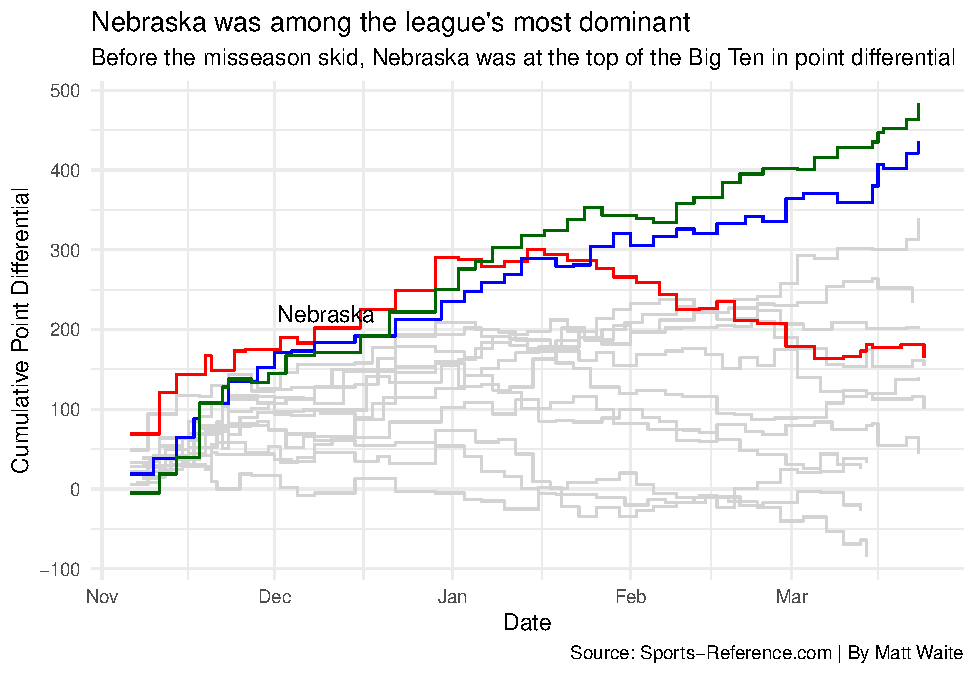
\includegraphics{SportsData_files/figure-latex/unnamed-chunk-151-1.pdf}

\chapter{Ridge charts}\label{ridge-charts}

Ridgeplots are useful for when you want to show how different groupings
compare with a large number of datapoints. So let's look at how we do
this, and in the process, we learn about ggplot extensions. The
extensions add functionality to ggplot, which doesn't out of the box
have ridgeplots (sometimes called joyplots).

In the console, run this: \texttt{install.packages("ggridges")}

Now we can add those libraries.

\begin{Shaded}
\begin{Highlighting}[]
\KeywordTok{library}\NormalTok{(tidyverse)}
\KeywordTok{library}\NormalTok{(ggridges)}
\end{Highlighting}
\end{Shaded}

So for this, let's look at every basketball game played since the
2014-15 season. That's more than 28,000 basketball games.
\href{https://unl.box.com/s/u9407jj007fxtnu1vbkybdawaqg6j3fw}{Download
that data here}.

\begin{Shaded}
\begin{Highlighting}[]
\NormalTok{logs <-}\StringTok{ }\KeywordTok{read_csv}\NormalTok{(}\StringTok{"data/logs1519.csv"}\NormalTok{)}
\end{Highlighting}
\end{Shaded}

\begin{verbatim}
## Warning: Missing column names filled in: 'X1' [1]
\end{verbatim}

\begin{verbatim}
## Parsed with column specification:
## cols(
##   .default = col_double(),
##   Date = col_date(format = ""),
##   HomeAway = col_character(),
##   Opponent = col_character(),
##   W_L = col_character(),
##   Blank = col_logical(),
##   Team = col_character(),
##   Conference = col_character(),
##   season = col_character()
## )
\end{verbatim}

\begin{verbatim}
## See spec(...) for full column specifications.
\end{verbatim}

So I want to group teams by wins. Wins are the only thing that matter --
ask Tim Miles. So our data has a column called W\_L that lists if the
team won or lost. The problem is it doens't just say W or L. If the game
went to overtime, it lists that. That complicates counting wins. And,
with ridgeplots, I want to be be able to separate EVERY GAME by how many
wins the team had over a SEASON. So I've got some work to do.

First, here's a trick to find a string of text and make that. It's
called \texttt{grepl} and the basic syntax is grepl for this string in
this field and then do what I tell you. In this case, we're going to
create a new field called winloss look for W or L (and ignore any OT
notation) and give wins a 1 and losses a 0.

\begin{Shaded}
\begin{Highlighting}[]
\NormalTok{winlosslogs <-}\StringTok{ }\NormalTok{logs }\OperatorTok\StringTok{ }\KeywordTok{mutate}\NormalTok{(}\DataTypeTok{winloss =} \KeywordTok{case_when}\NormalTok{(}
  \KeywordTok{grepl}\NormalTok{(}\StringTok{"W"}\NormalTok{, W_L) }\OperatorTok{~}\StringTok{ }\DecValTok{1}\NormalTok{, }
  \KeywordTok{grepl}\NormalTok{(}\StringTok{"L"}\NormalTok{, W_L) }\OperatorTok{~}\StringTok{ }\DecValTok{0}\NormalTok{)}
\NormalTok{)}
\end{Highlighting}
\end{Shaded}

Now I'm going to add up all the winlosses for each team, which should
give me the number of wins for each team.

\begin{Shaded}
\begin{Highlighting}[]
\NormalTok{winlosslogs }\OperatorTok\StringTok{ }\KeywordTok{group_by}\NormalTok{(Team, Conference, season) }\OperatorTok\StringTok{ }\KeywordTok{summarise}\NormalTok{(}\DataTypeTok{TeamWins =} \KeywordTok{sum}\NormalTok{(winloss)) ->}\StringTok{ }\NormalTok{teamseasonwins}
\end{Highlighting}
\end{Shaded}

Now that I have season win totals, I can join that data back to my log
data so each game has the total number of wins in each season.

\begin{Shaded}
\begin{Highlighting}[]
\NormalTok{winlosslogs }\OperatorTok\StringTok{ }\KeywordTok{left_join}\NormalTok{(teamseasonwins, }\DataTypeTok{by=}\KeywordTok{c}\NormalTok{(}\StringTok{"Team"}\NormalTok{, }\StringTok{"Conference"}\NormalTok{, }\StringTok{"season"}\NormalTok{)) ->}\StringTok{ }\NormalTok{wintotallogs}
\end{Highlighting}
\end{Shaded}

Now I can use that same \texttt{case\_when} logic to create some
groupings. So I want to group teams together by how many wins they had
over the season. For no good reason, I started with more than 25 wins,
then did groups of 5 down to 10 wins. If you had fewer than 10 wins, God
help your program.

\begin{Shaded}
\begin{Highlighting}[]
\NormalTok{wintotallogs }\OperatorTok\StringTok{ }\KeywordTok{mutate}\NormalTok{(}\DataTypeTok{grouping =} \KeywordTok{case_when}\NormalTok{(}
\NormalTok{  TeamWins }\OperatorTok{>}\StringTok{ }\DecValTok{25} \OperatorTok{~}\StringTok{ "More than 25 wins"}\NormalTok{,}
\NormalTok{  TeamWins }\OperatorTok{>=}\StringTok{ }\DecValTok{20} \OperatorTok{&}\StringTok{ }\NormalTok{TeamWins }\OperatorTok{<=}\DecValTok{25} \OperatorTok{~}\StringTok{ "20-25 wins"}\NormalTok{,}
\NormalTok{  TeamWins }\OperatorTok{>=}\StringTok{ }\DecValTok{15} \OperatorTok{&}\StringTok{ }\NormalTok{TeamWins }\OperatorTok{<=}\DecValTok{19} \OperatorTok{~}\StringTok{ "15-19 wins"}\NormalTok{,}
\NormalTok{  TeamWins }\OperatorTok{>=}\StringTok{ }\DecValTok{10} \OperatorTok{&}\StringTok{ }\NormalTok{TeamWins }\OperatorTok{<=}\DecValTok{14} \OperatorTok{~}\StringTok{ "10-14 wins"}\NormalTok{,}
\NormalTok{  TeamWins }\OperatorTok{<}\StringTok{ }\DecValTok{10} \OperatorTok{~}\StringTok{ "Less than 10 wins"}\NormalTok{)}
\NormalTok{) ->}\StringTok{ }\NormalTok{wintotalgroupinglogs}
\end{Highlighting}
\end{Shaded}

So my \texttt{wintotalgroupinglogs} table has each game, with a field
that gives the total number of wins each team had that season and
labeling each game with one of five groupings. I could use
\texttt{dplyr} to do group\_by on those five groups and find some things
out about them, but ridgeplots do that visually.

Let's look at the differences in rebounds by those five groups. Do teams
that win more than 25 games rebound better than teams that win fewer
games?

The answer might surprise you.

\begin{Shaded}
\begin{Highlighting}[]
\KeywordTok{ggplot}\NormalTok{(wintotalgroupinglogs, }\KeywordTok{aes}\NormalTok{(}\DataTypeTok{x =}\NormalTok{ TeamTotalRebounds, }\DataTypeTok{y =}\NormalTok{ grouping, }\DataTypeTok{fill =}\NormalTok{ grouping)) }\OperatorTok{+}
\StringTok{  }\KeywordTok{geom_density_ridges}\NormalTok{() }\OperatorTok{+}
\StringTok{  }\KeywordTok{theme_ridges}\NormalTok{() }\OperatorTok{+}\StringTok{ }
\StringTok{  }\KeywordTok{theme}\NormalTok{(}\DataTypeTok{legend.position =} \StringTok{"none"}\NormalTok{)}
\end{Highlighting}
\end{Shaded}

\begin{verbatim}
## Picking joint bandwidth of 0.88
\end{verbatim}

\begin{verbatim}
## Warning: Removed 2 rows containing non-finite values (stat_density_ridges).
\end{verbatim}

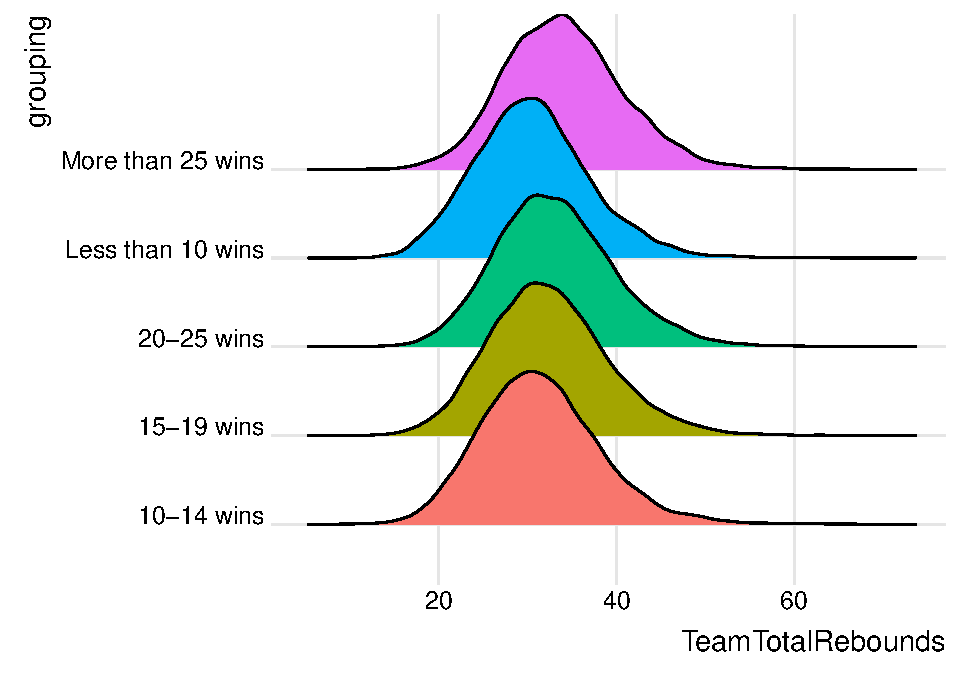
\includegraphics{SportsData_files/figure-latex/unnamed-chunk-158-1.pdf}

Answer? Not really. Game to game, maybe. Over five seasons? The
differences are indistiguishable.

How about assists?

\begin{Shaded}
\begin{Highlighting}[]
\KeywordTok{ggplot}\NormalTok{(wintotalgroupinglogs, }\KeywordTok{aes}\NormalTok{(}\DataTypeTok{x =}\NormalTok{ TeamAssists, }\DataTypeTok{y =}\NormalTok{ grouping, }\DataTypeTok{fill =}\NormalTok{ grouping)) }\OperatorTok{+}
\StringTok{  }\KeywordTok{geom_density_ridges}\NormalTok{() }\OperatorTok{+}
\StringTok{  }\KeywordTok{theme_ridges}\NormalTok{() }\OperatorTok{+}\StringTok{ }
\StringTok{  }\KeywordTok{theme}\NormalTok{(}\DataTypeTok{legend.position =} \StringTok{"none"}\NormalTok{)}
\end{Highlighting}
\end{Shaded}

\begin{verbatim}
## Picking joint bandwidth of 0.601
\end{verbatim}

\begin{verbatim}
## Warning: Removed 2 rows containing non-finite values (stat_density_ridges).
\end{verbatim}

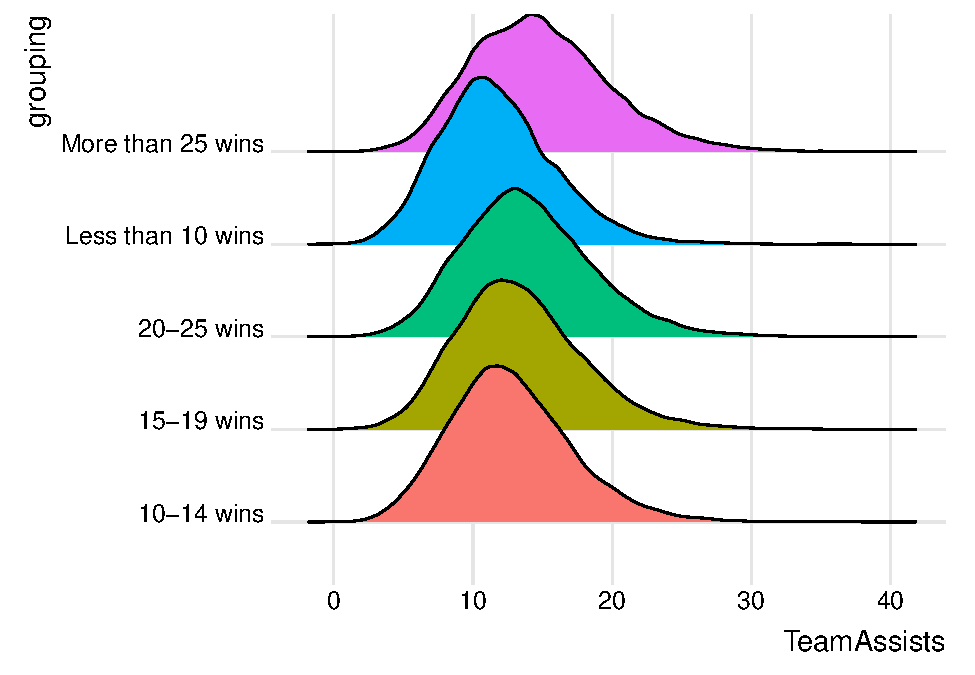
\includegraphics{SportsData_files/figure-latex/unnamed-chunk-159-1.pdf}

There's a little better, especially between top and bottom.

\begin{Shaded}
\begin{Highlighting}[]
\KeywordTok{ggplot}\NormalTok{(wintotalgroupinglogs, }\KeywordTok{aes}\NormalTok{(}\DataTypeTok{x =}\NormalTok{ Team3PPCT, }\DataTypeTok{y =}\NormalTok{ grouping, }\DataTypeTok{fill =}\NormalTok{ grouping)) }\OperatorTok{+}
\StringTok{  }\KeywordTok{geom_density_ridges}\NormalTok{() }\OperatorTok{+}
\StringTok{  }\KeywordTok{theme_ridges}\NormalTok{() }\OperatorTok{+}\StringTok{ }
\StringTok{  }\KeywordTok{theme}\NormalTok{(}\DataTypeTok{legend.position =} \StringTok{"none"}\NormalTok{)}
\end{Highlighting}
\end{Shaded}

\begin{verbatim}
## Picking joint bandwidth of 0.0156
\end{verbatim}

\begin{verbatim}
## Warning: Removed 2 rows containing non-finite values (stat_density_ridges).
\end{verbatim}

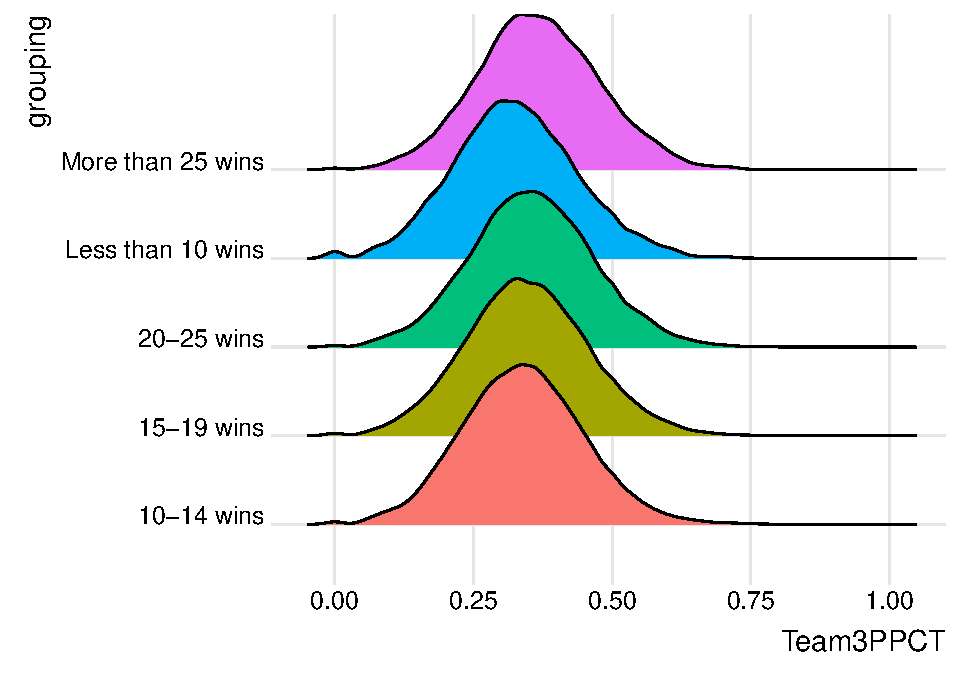
\includegraphics{SportsData_files/figure-latex/unnamed-chunk-160-1.pdf}

If you've been paying attention this semester, you know what's coming
next.

\begin{Shaded}
\begin{Highlighting}[]
\KeywordTok{ggplot}\NormalTok{(wintotalgroupinglogs, }\KeywordTok{aes}\NormalTok{(}\DataTypeTok{x =}\NormalTok{ TeamFGPCT, }\DataTypeTok{y =}\NormalTok{ grouping, }\DataTypeTok{fill =}\NormalTok{ grouping)) }\OperatorTok{+}
\StringTok{  }\KeywordTok{geom_density_ridges}\NormalTok{() }\OperatorTok{+}
\StringTok{  }\KeywordTok{theme_ridges}\NormalTok{() }\OperatorTok{+}\StringTok{ }
\StringTok{  }\KeywordTok{theme}\NormalTok{(}\DataTypeTok{legend.position =} \StringTok{"none"}\NormalTok{)}
\end{Highlighting}
\end{Shaded}

\begin{verbatim}
## Picking joint bandwidth of 0.0102
\end{verbatim}

\begin{verbatim}
## Warning: Removed 2 rows containing non-finite values (stat_density_ridges).
\end{verbatim}

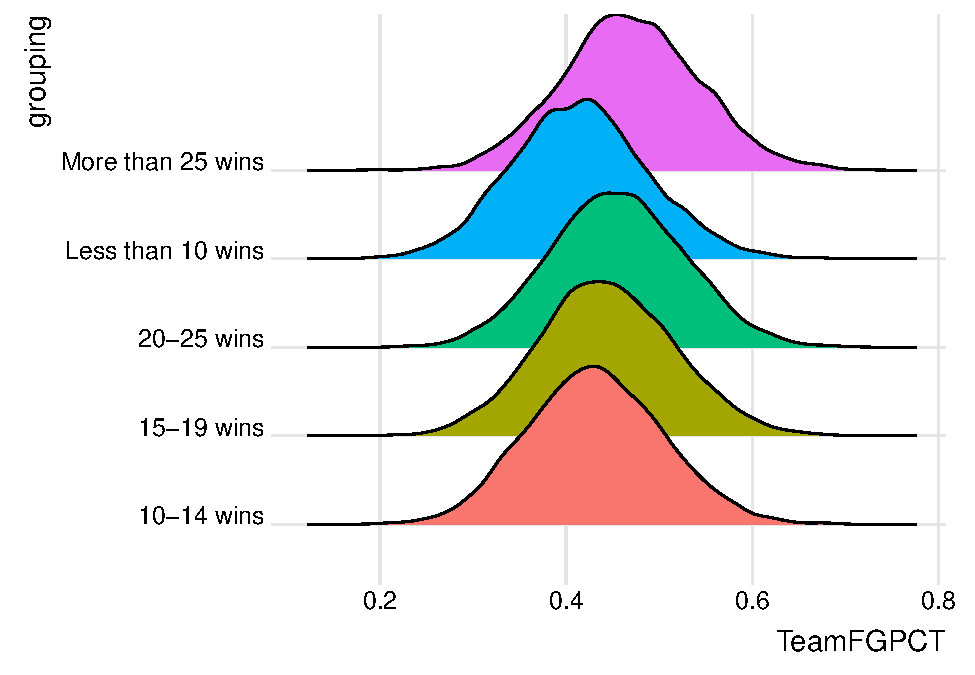
\includegraphics{SportsData_files/figure-latex/unnamed-chunk-161-1.pdf}

\chapter{Lollipop charts}\label{lollipop-charts}

Second to my love of waffle charts because I'm always hungry, lollipop
charts are an excellently named way of showing the difference between
two things on a number line -- a start and a finish, for instance. Or
the difference between two related things. Say, turnovers and assists.
They aren't a geom, specifically, but you can assemble them out of
points and segments, which are geoms.

\begin{Shaded}
\begin{Highlighting}[]
\KeywordTok{library}\NormalTok{(tidyverse)}
\end{Highlighting}
\end{Shaded}

\begin{Shaded}
\begin{Highlighting}[]
\NormalTok{logs <-}\StringTok{ }\KeywordTok{read_csv}\NormalTok{(}\StringTok{"data/logs19.csv"}\NormalTok{)}
\end{Highlighting}
\end{Shaded}

\begin{verbatim}
## Warning: Missing column names filled in: 'X1' [1]
\end{verbatim}

\begin{verbatim}
## Parsed with column specification:
## cols(
##   .default = col_double(),
##   Date = col_date(format = ""),
##   HomeAway = col_character(),
##   Opponent = col_character(),
##   W_L = col_character(),
##   Blank = col_logical(),
##   Team = col_character(),
##   Conference = col_character(),
##   season = col_character()
## )
\end{verbatim}

\begin{verbatim}
## See spec(...) for full column specifications.
\end{verbatim}

For the first example, let's look at the difference between a team's
shooting performance and the conference's shooting performance as a
whole. To get this, we're going to add up all the shots made by the
conference, all the attempts taken by the conference, and then mutate a
percentage based on that.

\begin{Shaded}
\begin{Highlighting}[]
\NormalTok{conferenceshooting <-}\StringTok{ }\NormalTok{logs }\OperatorTok\StringTok{ }\KeywordTok{group_by}\NormalTok{(Conference) }\OperatorTok\StringTok{ }\KeywordTok{summarise}\NormalTok{(}\DataTypeTok{totalshots =} \KeywordTok{sum}\NormalTok{(TeamFG), }\DataTypeTok{totalattempts =} \KeywordTok{sum}\NormalTok{(TeamFGA)) }\OperatorTok\StringTok{ }\KeywordTok{mutate}\NormalTok{(}\DataTypeTok{conferenceshootingpct =}\NormalTok{ totalshots}\OperatorTok{/}\NormalTok{totalattempts)}
\end{Highlighting}
\end{Shaded}

Now I'm going to do the same with teams.

\begin{Shaded}
\begin{Highlighting}[]
\NormalTok{teamshooting <-}\StringTok{ }\NormalTok{logs }\OperatorTok\StringTok{ }\KeywordTok{group_by}\NormalTok{(Team, Conference) }\OperatorTok\StringTok{ }\KeywordTok{summarise}\NormalTok{(}\DataTypeTok{totalshots =} \KeywordTok{sum}\NormalTok{(TeamFG), }\DataTypeTok{totalattempts =} \KeywordTok{sum}\NormalTok{(TeamFGA)) }\OperatorTok\StringTok{ }\KeywordTok{mutate}\NormalTok{(}\DataTypeTok{teamshootingpct =}\NormalTok{ totalshots}\OperatorTok{/}\NormalTok{totalattempts)}
\end{Highlighting}
\end{Shaded}

The last thing I need to do is join them together. So each team will
have the conference shooting percentage as well as their own.

\begin{Shaded}
\begin{Highlighting}[]
\NormalTok{shooting <-}\StringTok{ }\NormalTok{teamshooting }\OperatorTok\StringTok{ }\KeywordTok{left_join}\NormalTok{(conferenceshooting, }\DataTypeTok{by=}\StringTok{"Conference"}\NormalTok{)}
\end{Highlighting}
\end{Shaded}

I have every team in college basketball, but that's insane.

\begin{Shaded}
\begin{Highlighting}[]
\NormalTok{big10 <-}\StringTok{ }\NormalTok{shooting }\OperatorTok\StringTok{ }\KeywordTok{filter}\NormalTok{(Conference }\OperatorTok{==}\StringTok{ "Big Ten"}\NormalTok{)}
\end{Highlighting}
\end{Shaded}

So this takes a little doing, but the logic is pretty clear in the end.

A lollipop chart is made up of two things -- a line between two points,
and two points. So we need a geom\_segment and two geom\_points. And
because they get layered starting at the bottom, our segment is first. A
geom segment is made up of two things -- an x and a y value, and an x
and y end. In this case, our x and xend are the same -- the Team -- and
our y and yend are our two stats. For our points, both x values are the
Team and the y is the different stats. What that does is put each point
on the same line.

\begin{Shaded}
\begin{Highlighting}[]
\KeywordTok{ggplot}\NormalTok{(big10) }\OperatorTok{+}
\StringTok{  }\KeywordTok{geom_segment}\NormalTok{(}\KeywordTok{aes}\NormalTok{(}\DataTypeTok{x=}\NormalTok{Team, }\DataTypeTok{xend=}\NormalTok{Team, }\DataTypeTok{y=}\NormalTok{teamshootingpct, }\DataTypeTok{yend=}\NormalTok{conferenceshootingpct), }\DataTypeTok{color=}\StringTok{"grey"}\NormalTok{) }\OperatorTok{+}\StringTok{ }
\StringTok{  }\KeywordTok{geom_point}\NormalTok{(}\KeywordTok{aes}\NormalTok{(}\DataTypeTok{x=}\NormalTok{Team, }\DataTypeTok{y=}\NormalTok{teamshootingpct), }\DataTypeTok{color=}\StringTok{"red"}\NormalTok{) }\OperatorTok{+}\StringTok{ }
\StringTok{  }\KeywordTok{geom_point}\NormalTok{(}\KeywordTok{aes}\NormalTok{(}\DataTypeTok{x=}\NormalTok{Team, }\DataTypeTok{y=}\NormalTok{conferenceshootingpct), }\DataTypeTok{color=}\StringTok{"blue"}\NormalTok{) }\OperatorTok{+}
\StringTok{  }\KeywordTok{coord_flip}\NormalTok{()}
\end{Highlighting}
\end{Shaded}

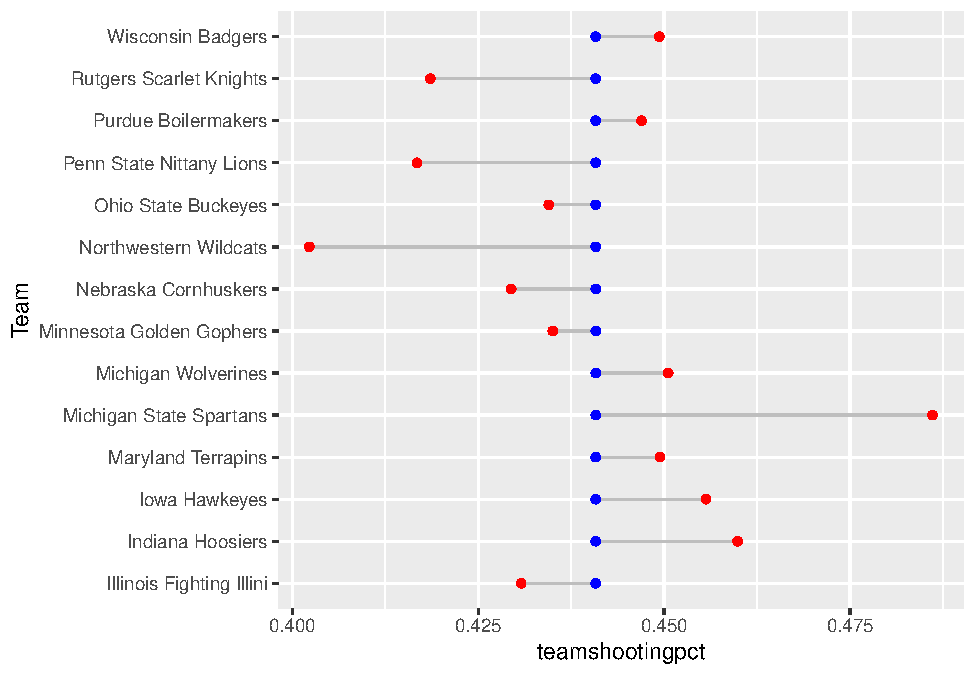
\includegraphics{SportsData_files/figure-latex/unnamed-chunk-168-1.pdf}

We can do better by changing the order of the teams by their shooting
performance and giving it some theme love.

\begin{Shaded}
\begin{Highlighting}[]
\KeywordTok{ggplot}\NormalTok{(big10) }\OperatorTok{+}
\StringTok{  }\KeywordTok{geom_segment}\NormalTok{(}\KeywordTok{aes}\NormalTok{(}\DataTypeTok{x=}\KeywordTok{reorder}\NormalTok{(Team, teamshootingpct), }\DataTypeTok{xend=}\NormalTok{Team, }\DataTypeTok{y=}\NormalTok{teamshootingpct, }\DataTypeTok{yend=}\NormalTok{conferenceshootingpct), }\DataTypeTok{color=}\StringTok{"grey"}\NormalTok{) }\OperatorTok{+}\StringTok{ }
\StringTok{  }\KeywordTok{geom_point}\NormalTok{(}\KeywordTok{aes}\NormalTok{(}\DataTypeTok{x=}\KeywordTok{reorder}\NormalTok{(Team, teamshootingpct), }\DataTypeTok{y=}\NormalTok{teamshootingpct), }\DataTypeTok{color=}\StringTok{"red"}\NormalTok{) }\OperatorTok{+}\StringTok{ }
\StringTok{  }\KeywordTok{geom_point}\NormalTok{(}\KeywordTok{aes}\NormalTok{(}\DataTypeTok{x=}\KeywordTok{reorder}\NormalTok{(Team, teamshootingpct), }\DataTypeTok{y=}\NormalTok{conferenceshootingpct), }\DataTypeTok{color=}\StringTok{"blue"}\NormalTok{) }\OperatorTok{+}
\StringTok{  }\KeywordTok{coord_flip}\NormalTok{() }\OperatorTok{+}
\StringTok{   }\KeywordTok{labs}\NormalTok{(}\DataTypeTok{x=}\StringTok{""}\NormalTok{, }\DataTypeTok{y=}\StringTok{"Shooting percentage vs league average"}\NormalTok{, }\DataTypeTok{title=}\StringTok{"Except Purdue, shooting predicted Big Ten success"}\NormalTok{, }\DataTypeTok{subtitle=}\StringTok{"The Boilermakers were average shooters, went deep in the NCAA tournament"}\NormalTok{, }\DataTypeTok{caption=}\StringTok{"Source: sports-reference.com | By Matt Waite"}\NormalTok{) }\OperatorTok{+}
\StringTok{  }\KeywordTok{theme_minimal}\NormalTok{() }\OperatorTok{+}\StringTok{ }
\StringTok{  }\KeywordTok{theme}\NormalTok{(}
    \DataTypeTok{plot.title =} \KeywordTok{element_text}\NormalTok{(}\DataTypeTok{size =} \DecValTok{16}\NormalTok{, }\DataTypeTok{face =} \StringTok{"bold"}\NormalTok{, }\DataTypeTok{hjust =} \DecValTok{1}\NormalTok{),}
    \DataTypeTok{plot.subtitle =} \KeywordTok{element_text}\NormalTok{(}\DataTypeTok{hjust =} \FloatTok{1.3}\NormalTok{),}
    \DataTypeTok{axis.title =} \KeywordTok{element_text}\NormalTok{(}\DataTypeTok{size =} \DecValTok{10}\NormalTok{),}
    \DataTypeTok{axis.title.y =} \KeywordTok{element_blank}\NormalTok{(),}
    \DataTypeTok{axis.text =} \KeywordTok{element_text}\NormalTok{(}\DataTypeTok{size =} \DecValTok{7}\NormalTok{),}
    \DataTypeTok{axis.ticks =} \KeywordTok{element_blank}\NormalTok{()}
\NormalTok{  )}
\end{Highlighting}
\end{Shaded}

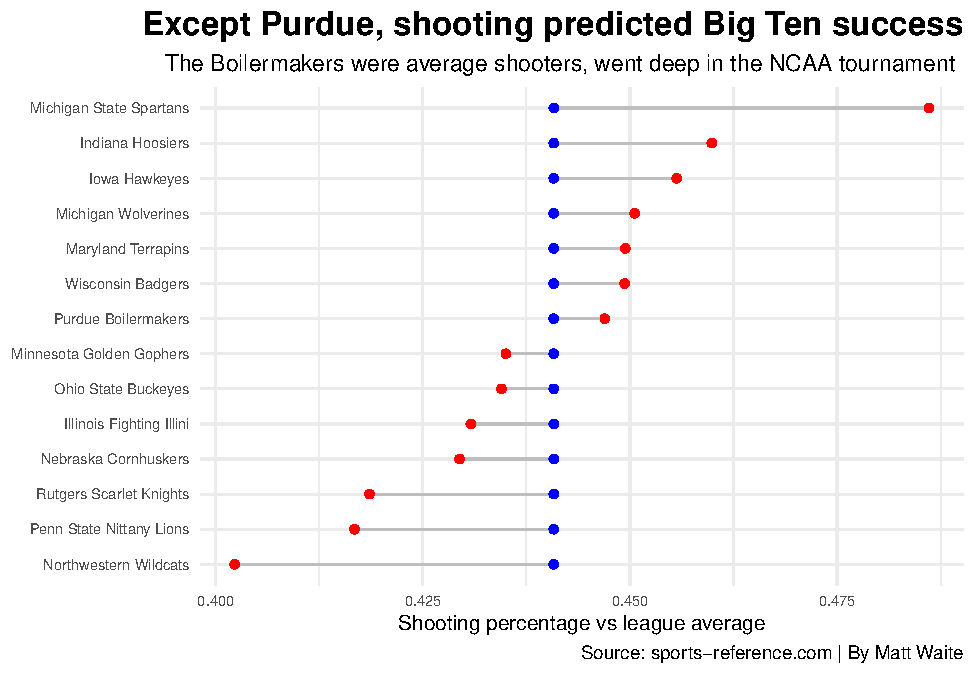
\includegraphics{SportsData_files/figure-latex/unnamed-chunk-169-1.pdf}

What if we wanted to order them by wins? Our data has a column called
W\_L that lists if the team won or lost. The problem is it doens't just
say W or L. If the game went to overtime, it lists that. That
complicates counting wins. Here's a trick to find a string of text and
make that. It's called \texttt{grepl} and the basic syntax is grepl for
this string in this field and then do what I tell you. In this case,
we're going to create a new field called winloss look for W or L (and
ignore any OT notation) and give wins a 1 and losses a 0.

\begin{Shaded}
\begin{Highlighting}[]
\NormalTok{winlosslogs <-}\StringTok{ }\NormalTok{logs }\OperatorTok\StringTok{ }\KeywordTok{mutate}\NormalTok{(}\DataTypeTok{winloss =} \KeywordTok{case_when}\NormalTok{(}
  \KeywordTok{grepl}\NormalTok{(}\StringTok{"W"}\NormalTok{, W_L) }\OperatorTok{~}\StringTok{ }\DecValTok{1}\NormalTok{, }
  \KeywordTok{grepl}\NormalTok{(}\StringTok{"L"}\NormalTok{, W_L) }\OperatorTok{~}\StringTok{ }\DecValTok{0}\NormalTok{)}
\NormalTok{)}
\end{Highlighting}
\end{Shaded}

So let's look at turnovers and assists. We'll call it give and take.
Does the difference between those two things indicate something when we
sort them by wins?

\begin{Shaded}
\begin{Highlighting}[]
\NormalTok{giveandtake <-}\StringTok{ }\NormalTok{winlosslogs }\OperatorTok\StringTok{ }\KeywordTok{group_by}\NormalTok{(Conference, Team) }\OperatorTok\StringTok{ }\KeywordTok{summarise}\NormalTok{(}\DataTypeTok{turnovers =} \KeywordTok{sum}\NormalTok{(TeamTurnovers), }\DataTypeTok{assists =} \KeywordTok{sum}\NormalTok{(TeamAssists), }\DataTypeTok{wins=}\KeywordTok{sum}\NormalTok{(winloss)) }
\end{Highlighting}
\end{Shaded}

\begin{Shaded}
\begin{Highlighting}[]
\NormalTok{big10gt <-}\StringTok{ }\NormalTok{giveandtake }\OperatorTok\StringTok{ }\KeywordTok{filter}\NormalTok{(Conference }\OperatorTok{==}\StringTok{ "Big Ten"}\NormalTok{)}
\end{Highlighting}
\end{Shaded}

\begin{Shaded}
\begin{Highlighting}[]
\KeywordTok{ggplot}\NormalTok{(big10gt) }\OperatorTok{+}
\StringTok{  }\KeywordTok{geom_segment}\NormalTok{(}\KeywordTok{aes}\NormalTok{(}\DataTypeTok{x=}\KeywordTok{reorder}\NormalTok{(Team, wins), }\DataTypeTok{xend=}\NormalTok{Team, }\DataTypeTok{y=}\NormalTok{turnovers, }\DataTypeTok{yend=}\NormalTok{assists), }\DataTypeTok{color=}\StringTok{"grey"}\NormalTok{) }\OperatorTok{+}\StringTok{ }
\StringTok{  }\KeywordTok{geom_point}\NormalTok{(}\KeywordTok{aes}\NormalTok{(}\DataTypeTok{x=}\KeywordTok{reorder}\NormalTok{(Team, wins), }\DataTypeTok{y=}\NormalTok{turnovers), }\DataTypeTok{color=}\StringTok{"red"}\NormalTok{) }\OperatorTok{+}\StringTok{ }
\StringTok{  }\KeywordTok{geom_point}\NormalTok{(}\KeywordTok{aes}\NormalTok{(}\DataTypeTok{x=}\KeywordTok{reorder}\NormalTok{(Team, wins), }\DataTypeTok{y=}\NormalTok{assists), }\DataTypeTok{color=}\StringTok{"blue"}\NormalTok{) }\OperatorTok{+}
\StringTok{  }\KeywordTok{coord_flip}\NormalTok{()}
\end{Highlighting}
\end{Shaded}

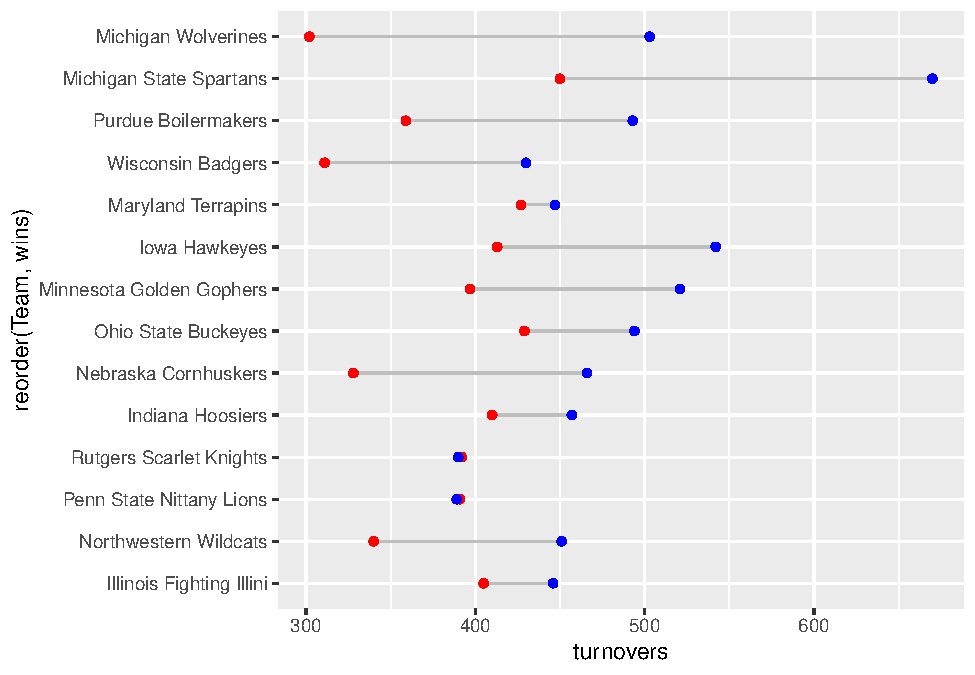
\includegraphics{SportsData_files/figure-latex/unnamed-chunk-173-1.pdf}

Short answer: Not really.

\chapter{Scatterplots}\label{scatterplots}

In several chapters of this book, we've been fixated on the Nebraska
basketball team's shooting percentage, which took a nose dive during the
season and ultimately doomed Tim Miles job. The question is \ldots{}
does it matter?

This is what we're going to start to answer today. And we'll do it with
scatterplots and correlations.

First, we need libraries and
\href{https://unl.box.com/s/a8m91bro10t89watsyo13yjegb1fy009}{data}.

\begin{Shaded}
\begin{Highlighting}[]
\KeywordTok{library}\NormalTok{(tidyverse)}
\end{Highlighting}
\end{Shaded}

\begin{Shaded}
\begin{Highlighting}[]
\NormalTok{logs <-}\StringTok{ }\KeywordTok{read_csv}\NormalTok{(}\StringTok{"data/logs19.csv"}\NormalTok{)}
\end{Highlighting}
\end{Shaded}

\begin{verbatim}
## Warning: Missing column names filled in: 'X1' [1]
\end{verbatim}

\begin{verbatim}
## Parsed with column specification:
## cols(
##   .default = col_double(),
##   Date = col_date(format = ""),
##   HomeAway = col_character(),
##   Opponent = col_character(),
##   W_L = col_character(),
##   Blank = col_logical(),
##   Team = col_character(),
##   Conference = col_character(),
##   season = col_character()
## )
\end{verbatim}

\begin{verbatim}
## See spec(...) for full column specifications.
\end{verbatim}

To do this, we need all teams and their season stats. How much, over the
course of a season, does a thing matter? That's the question you're
going to answer.

In our case, we want to know how much does shooting percentage influence
wins? How much different can we explain in wins with shooting
percentage? We're going to total up the number of wins each team has and
their season shooting percentage in one swoop.

Let's borrow from our ridgecharts work to get the correct wins and
losses totals for each team.

\begin{Shaded}
\begin{Highlighting}[]
\NormalTok{winlosslogs <-}\StringTok{ }\NormalTok{logs }\OperatorTok\StringTok{ }\KeywordTok{mutate}\NormalTok{(}\DataTypeTok{winloss =} \KeywordTok{case_when}\NormalTok{(}
  \KeywordTok{grepl}\NormalTok{(}\StringTok{"W"}\NormalTok{, W_L) }\OperatorTok{~}\StringTok{ }\DecValTok{1}\NormalTok{, }
  \KeywordTok{grepl}\NormalTok{(}\StringTok{"L"}\NormalTok{, W_L) }\OperatorTok{~}\StringTok{ }\DecValTok{0}\NormalTok{)}
\NormalTok{)}
\end{Highlighting}
\end{Shaded}

Now we can get a dataframe together that gives us the total wins for
each team, and the total shots taken and made, which let's us calculate
a season shooting percentage.

\begin{Shaded}
\begin{Highlighting}[]
\NormalTok{winlosslogs }\OperatorTok\StringTok{ }
\StringTok{  }\KeywordTok{group_by}\NormalTok{(Team) }\OperatorTok
\StringTok{  }\KeywordTok{summarise}\NormalTok{(}
    \DataTypeTok{wins =} \KeywordTok{sum}\NormalTok{(winloss),}
    \DataTypeTok{totalFGAttempts =} \KeywordTok{sum}\NormalTok{(TeamFGA),}
    \DataTypeTok{totalFG =} \KeywordTok{sum}\NormalTok{(TeamFG)}
\NormalTok{  ) }\OperatorTok
\StringTok{  }\KeywordTok{mutate}\NormalTok{(}\DataTypeTok{fgpct =}\NormalTok{ totalFG}\OperatorTok{/}\NormalTok{totalFGAttempts) ->}\StringTok{ }\NormalTok{fgmodel}
\end{Highlighting}
\end{Shaded}

Now let's look at the scatterplot. With a scatterplot, we put what
predicts the thing on the X axis, and the thing being predicted on the Y
axis. In this case, X is our shooting percentage, y is our wins.

\begin{Shaded}
\begin{Highlighting}[]
\KeywordTok{ggplot}\NormalTok{(fgmodel, }\KeywordTok{aes}\NormalTok{(}\DataTypeTok{x=}\NormalTok{fgpct, }\DataTypeTok{y=}\NormalTok{wins)) }\OperatorTok{+}\StringTok{ }\KeywordTok{geom_point}\NormalTok{()}
\end{Highlighting}
\end{Shaded}

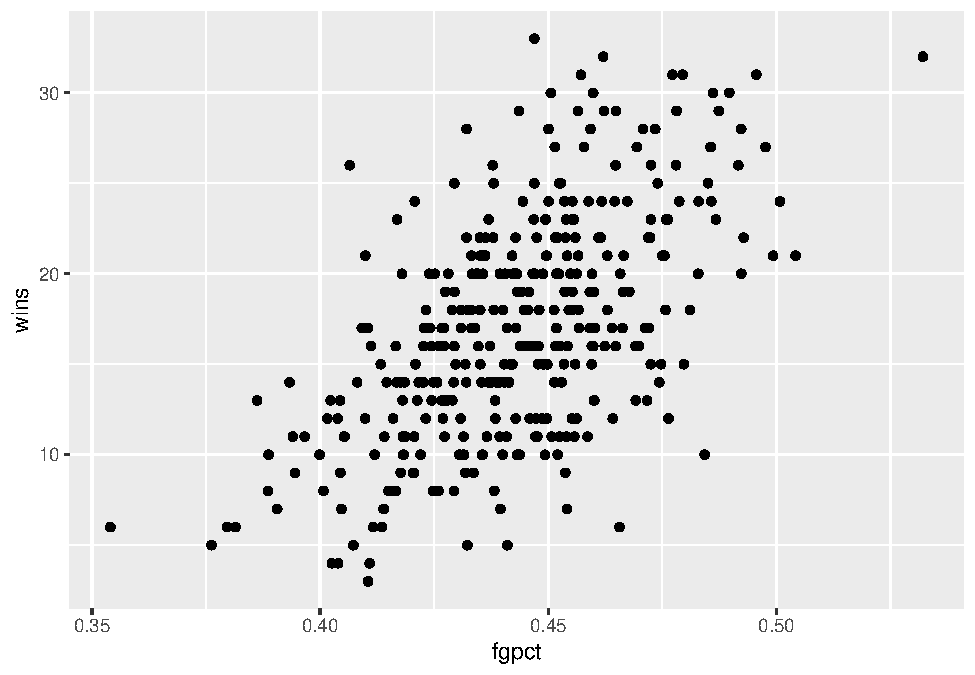
\includegraphics{SportsData_files/figure-latex/unnamed-chunk-178-1.pdf}

Let's talk about this. It seems that the data slopes up to the right.
That would indicate a positive correlation between shooting percentage
and wins. And that makes sense, no? You'd expect teams that shoot the
ball well to win. But can we get a better sense of this? Yes, by adding
another geom -- \texttt{geom\_smooth}.

\begin{Shaded}
\begin{Highlighting}[]
\KeywordTok{ggplot}\NormalTok{(fgmodel, }\KeywordTok{aes}\NormalTok{(}\DataTypeTok{x=}\NormalTok{fgpct, }\DataTypeTok{y=}\NormalTok{wins)) }\OperatorTok{+}\StringTok{ }\KeywordTok{geom_point}\NormalTok{() }\OperatorTok{+}\StringTok{ }\KeywordTok{geom_smooth}\NormalTok{(}\DataTypeTok{method=}\NormalTok{lm, }\DataTypeTok{se=}\OtherTok{TRUE}\NormalTok{)}
\end{Highlighting}
\end{Shaded}

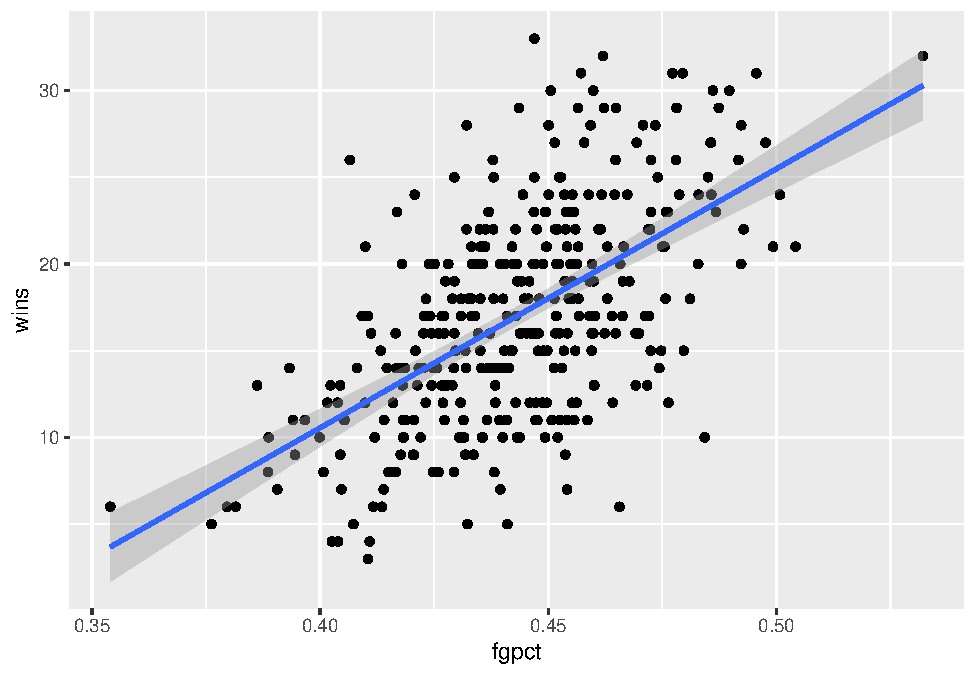
\includegraphics{SportsData_files/figure-latex/unnamed-chunk-179-1.pdf}

But \ldots{} how strong a relationship is this? How much can shooting
percentage explain wins? Can we put some numbers to this?

Of course we can. We can apply a linear model to this -- remember
Chapter 8? We're going to create an object called fit, and then we're
going to put into that object a linear model -- \texttt{lm} -- and the
way to read this is ``wins are predicted by field goal percentage''.
Then we just want the summary of that model.

\begin{Shaded}
\begin{Highlighting}[]
\NormalTok{fit <-}\StringTok{ }\KeywordTok{lm}\NormalTok{(wins }\OperatorTok{~}\StringTok{ }\NormalTok{fgpct, }\DataTypeTok{data =}\NormalTok{ fgmodel)}
\KeywordTok{summary}\NormalTok{(fit)}
\end{Highlighting}
\end{Shaded}

\begin{verbatim}
## 
## Call:
## lm(formula = wins ~ fgpct, data = fgmodel)
## 
## Residuals:
##      Min       1Q   Median       3Q      Max 
## -14.3536  -3.4523  -0.1125   3.3834  15.4318 
## 
## Coefficients:
##             Estimate Std. Error t value Pr(>|t|)    
## (Intercept)  -49.217      4.845  -10.16   <2e-16 ***
## fgpct        149.416     10.915   13.69   <2e-16 ***
## ---
## Signif. codes:  0 '***' 0.001 '**' 0.01 '*' 0.05 '.' 0.1 ' ' 1
## 
## Residual standard error: 5.035 on 351 degrees of freedom
## Multiple R-squared:  0.348,  Adjusted R-squared:  0.3462 
## F-statistic: 187.4 on 1 and 351 DF,  p-value: < 2.2e-16
\end{verbatim}

Remember from Chapter 8: There's just a few things you really need.

The first thing: R-squared. In this case, the Adjusted R-squared value
is .3462, which we can interpret as shooting percentage predicts about
35 percent of the variance in wins. Which sounds not great, but in
social science, that's huge. That's great. A psychology major would
murder for that R-squared.

Second: The P-value. We want anything less than .05. If it's above .05,
the change between them is not statistically significant -- it's
probably explained by random chance. In our case, we have 2.2e-16, which
is to say 2.2 with 16 zeros in front of it, or .000000000000000022. Is
that less than .05? Yes. Yes it is. So this is not random. Again, we
would expect this, so it's a good logic test.

Third: The coefficient. In this case, the coefficient for fgpct is
149.416. Since I didn't convert percentages to decimals, what this says
is that for every perentage point improvement in shooting percentage, we
can expect the team to win 1.49 more games plus or minus some error.

And we can use this to predict a team's wins: remember your algebra and
y = mx + b. In this case, y is the wins, m is the coefficient, x is the
shooting percentage and b is the intercept.

So can plug these together: Expected wins = 149.416 * shooting
percentage - 49.217

Let's use Nebraska as an example. They shot about .43 on the season
(.4294421 to be exact).

y = 149.416 * .4294421 - 49.217 or 14.95 wins. How many wins did
Nebraska have? 19.

What does that mean? It means that as disappointing a season as it was,
Nebraska actually OVERPERFORMED it's season shooting percentage. They
shouldn't have won as many games as they did.

\chapter{Facet wraps}\label{facet-wraps}

Sometimes the easiest way to spot a trend is to chart a bunch of small
things side by side. Edward Tufte calls this ``small multiples'' where
ggplot calls this a facet wrap or a facet grid, depending.

One thing we noticed earlier in the semester -- it seems that a lot of
teams shoot worse as the season goes on. Do they? We could answer this a
number of ways, but the best way to show people would be visually. Let's
use Small Mulitples.

As always, we start with libraries.

\begin{Shaded}
\begin{Highlighting}[]
\KeywordTok{library}\NormalTok{(tidyverse)}
\end{Highlighting}
\end{Shaded}

Now data.

\begin{Shaded}
\begin{Highlighting}[]
\NormalTok{logs <-}\StringTok{ }\KeywordTok{read_csv}\NormalTok{(}\StringTok{"data/logs19.csv"}\NormalTok{)}
\end{Highlighting}
\end{Shaded}

\begin{verbatim}
## Warning: Missing column names filled in: 'X1' [1]
\end{verbatim}

\begin{verbatim}
## Parsed with column specification:
## cols(
##   .default = col_double(),
##   Date = col_date(format = ""),
##   HomeAway = col_character(),
##   Opponent = col_character(),
##   W_L = col_character(),
##   Blank = col_logical(),
##   Team = col_character(),
##   Conference = col_character(),
##   season = col_character()
## )
\end{verbatim}

\begin{verbatim}
## See spec(...) for full column specifications.
\end{verbatim}

Let's narrow our pile and look just at the Big Ten.

\begin{Shaded}
\begin{Highlighting}[]
\NormalTok{big10 <-}\StringTok{ }\NormalTok{logs }\OperatorTok\StringTok{ }\KeywordTok{filter}\NormalTok{(Conference }\OperatorTok{==}\StringTok{ "Big Ten"}\NormalTok{)}
\end{Highlighting}
\end{Shaded}

The first thing we can do is look at a line chart, like we have done in
previous chapters.

\begin{Shaded}
\begin{Highlighting}[]
\KeywordTok{ggplot}\NormalTok{() }\OperatorTok{+}\StringTok{ }\KeywordTok{geom_line}\NormalTok{(}\DataTypeTok{data=}\NormalTok{big10, }\KeywordTok{aes}\NormalTok{(}\DataTypeTok{x=}\NormalTok{Date, }\DataTypeTok{y=}\NormalTok{TeamFGPCT, }\DataTypeTok{group=}\NormalTok{Team)) }\OperatorTok{+}\StringTok{ }\KeywordTok{scale_y_continuous}\NormalTok{(}\DataTypeTok{limits =} \KeywordTok{c}\NormalTok{(}\DecValTok{0}\NormalTok{, .}\DecValTok{7}\NormalTok{))}
\end{Highlighting}
\end{Shaded}

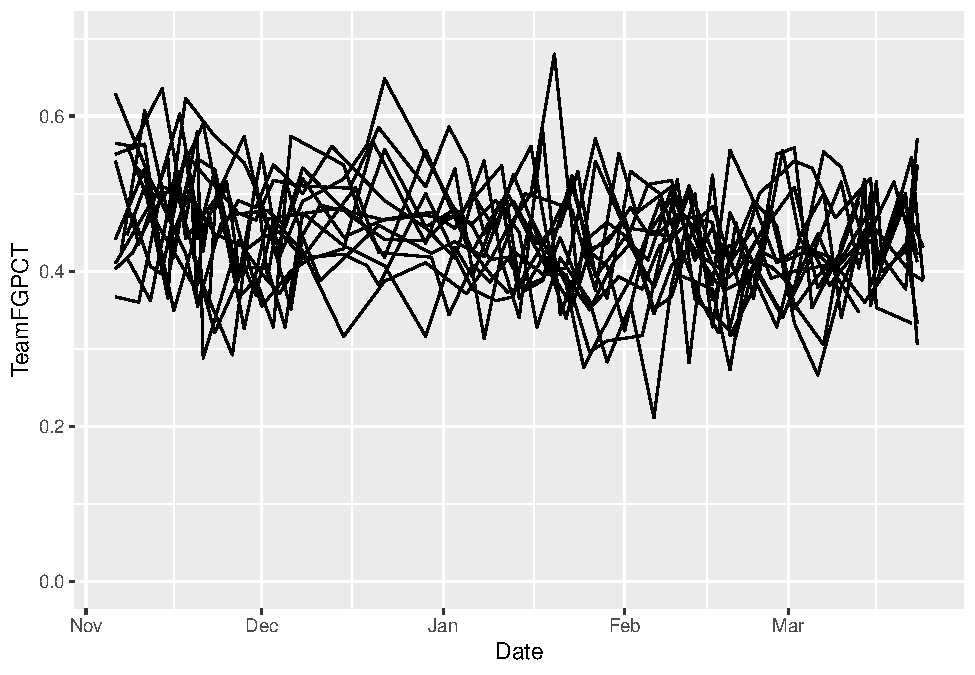
\includegraphics{SportsData_files/figure-latex/unnamed-chunk-184-1.pdf}

And, not surprisingly, we get a hairball. We could color certain lines,
but that would limit us to focus on one team. What if we did all of them
at once? We do that with a \texttt{facet\_wrap}. The only thing we MUST
pass into a \texttt{facet\_wrap} is what thing we're going to separate
them out by. In this case, we preceed that field with a tilde, so in our
case we want the Team field. It looks like this:

\begin{Shaded}
\begin{Highlighting}[]
\KeywordTok{ggplot}\NormalTok{() }\OperatorTok{+}\StringTok{ }\KeywordTok{geom_line}\NormalTok{(}\DataTypeTok{data=}\NormalTok{big10, }\KeywordTok{aes}\NormalTok{(}\DataTypeTok{x=}\NormalTok{Date, }\DataTypeTok{y=}\NormalTok{TeamFGPCT, }\DataTypeTok{group=}\NormalTok{Team)) }\OperatorTok{+}\StringTok{ }\KeywordTok{scale_y_continuous}\NormalTok{(}\DataTypeTok{limits =} \KeywordTok{c}\NormalTok{(}\DecValTok{0}\NormalTok{, .}\DecValTok{7}\NormalTok{)) }\OperatorTok{+}\StringTok{ }\KeywordTok{facet_wrap}\NormalTok{(}\OperatorTok{~}\NormalTok{Team)}
\end{Highlighting}
\end{Shaded}

\includegraphics{SportsData_files/figure-latex/unnamed-chunk-185-1.pdf}

Answer: Not immediately clear, but we can look at this and analyze it.
We could add a peice of annotation to help us out.

\begin{Shaded}
\begin{Highlighting}[]
\NormalTok{big10 }\OperatorTok\StringTok{ }\KeywordTok{summarise}\NormalTok{(}\KeywordTok{mean}\NormalTok{(TeamFGPCT))}
\end{Highlighting}
\end{Shaded}

\begin{verbatim}
## # A tibble: 1 x 1
##   `mean(TeamFGPCT)`
##               <dbl>
## 1             0.442
\end{verbatim}

\begin{Shaded}
\begin{Highlighting}[]
\KeywordTok{ggplot}\NormalTok{() }\OperatorTok{+}\StringTok{ }\KeywordTok{geom_hline}\NormalTok{(}\DataTypeTok{yintercept=}\NormalTok{.}\DecValTok{4447}\NormalTok{, }\DataTypeTok{color=}\StringTok{"dark grey"}\NormalTok{) }\OperatorTok{+}\StringTok{ }\KeywordTok{geom_line}\NormalTok{(}\DataTypeTok{data=}\NormalTok{big10, }\KeywordTok{aes}\NormalTok{(}\DataTypeTok{x=}\NormalTok{Date, }\DataTypeTok{y=}\NormalTok{TeamFGPCT, }\DataTypeTok{group=}\NormalTok{Team)) }\OperatorTok{+}\StringTok{ }\KeywordTok{scale_y_continuous}\NormalTok{(}\DataTypeTok{limits =} \KeywordTok{c}\NormalTok{(}\DecValTok{0}\NormalTok{, .}\DecValTok{7}\NormalTok{)) }\OperatorTok{+}\StringTok{ }\KeywordTok{facet_wrap}\NormalTok{(}\OperatorTok{~}\NormalTok{Team)}
\end{Highlighting}
\end{Shaded}

\includegraphics{SportsData_files/figure-latex/unnamed-chunk-187-1.pdf}

What do you see here? How do teams compare? How do they change over
time? I'm not asking you these questions because they're an assignment
-- I'm asking because that's exactly what this chart helps answer. Your
brain will immediately start making those connections.

\section{Facet grid vs facet wraps}\label{facet-grid-vs-facet-wraps}

Facet grids allow us to put teams on the same plane, versus just
repeating them. And we can specify that plane as vertical or horizontal.
For example, here's our chart from above, but using facet\_grid to stack
them.

\begin{Shaded}
\begin{Highlighting}[]
\KeywordTok{ggplot}\NormalTok{() }\OperatorTok{+}\StringTok{ }\KeywordTok{geom_hline}\NormalTok{(}\DataTypeTok{yintercept=}\NormalTok{.}\DecValTok{4447}\NormalTok{, }\DataTypeTok{color=}\StringTok{"dark grey"}\NormalTok{) }\OperatorTok{+}\StringTok{ }\KeywordTok{geom_line}\NormalTok{(}\DataTypeTok{data=}\NormalTok{big10, }\KeywordTok{aes}\NormalTok{(}\DataTypeTok{x=}\NormalTok{Date, }\DataTypeTok{y=}\NormalTok{TeamFGPCT, }\DataTypeTok{group=}\NormalTok{Team)) }\OperatorTok{+}\StringTok{ }\KeywordTok{scale_y_continuous}\NormalTok{(}\DataTypeTok{limits =} \KeywordTok{c}\NormalTok{(}\DecValTok{0}\NormalTok{, .}\DecValTok{7}\NormalTok{)) }\OperatorTok{+}\StringTok{ }\KeywordTok{facet_grid}\NormalTok{(Team }\OperatorTok{~}\StringTok{ }\NormalTok{.)}
\end{Highlighting}
\end{Shaded}

\includegraphics{SportsData_files/figure-latex/unnamed-chunk-188-1.pdf}

And here they are next to each other:

\begin{Shaded}
\begin{Highlighting}[]
\KeywordTok{ggplot}\NormalTok{() }\OperatorTok{+}\StringTok{ }\KeywordTok{geom_hline}\NormalTok{(}\DataTypeTok{yintercept=}\NormalTok{.}\DecValTok{4447}\NormalTok{, }\DataTypeTok{color=}\StringTok{"dark grey"}\NormalTok{) }\OperatorTok{+}\StringTok{ }\KeywordTok{geom_line}\NormalTok{(}\DataTypeTok{data=}\NormalTok{big10, }\KeywordTok{aes}\NormalTok{(}\DataTypeTok{x=}\NormalTok{Date, }\DataTypeTok{y=}\NormalTok{TeamFGPCT, }\DataTypeTok{group=}\NormalTok{Team)) }\OperatorTok{+}\StringTok{ }\KeywordTok{scale_y_continuous}\NormalTok{(}\DataTypeTok{limits =} \KeywordTok{c}\NormalTok{(}\DecValTok{0}\NormalTok{, .}\DecValTok{7}\NormalTok{)) }\OperatorTok{+}\StringTok{ }\KeywordTok{facet_grid}\NormalTok{(. }\OperatorTok{~}\StringTok{ }\NormalTok{Team)}
\end{Highlighting}
\end{Shaded}

\includegraphics{SportsData_files/figure-latex/unnamed-chunk-189-1.pdf}

Note: We'd have some work to do with the labeling on this -- we'll get
to that -- but you can see where this is valuable comparing a group of
things. One warning: Don't go too crazy with this or it loses it's
visual power.

\section{Other types}\label{other-types}

Line charts aren't the only things we can do. We can do any kind of
chart in ggplot. Staying with shooting, where are team's winning and
losing performances coming fromwhen we talk about team shooting and
opponent shooting?

\begin{Shaded}
\begin{Highlighting}[]
\KeywordTok{ggplot}\NormalTok{() }\OperatorTok{+}\StringTok{ }\KeywordTok{geom_point}\NormalTok{(}\DataTypeTok{data=}\NormalTok{big10, }\KeywordTok{aes}\NormalTok{(}\DataTypeTok{x=}\NormalTok{TeamFGPCT, }\DataTypeTok{y=}\NormalTok{OpponentFGPCT, }\DataTypeTok{color=}\NormalTok{W_L)) }\OperatorTok{+}\StringTok{ }\KeywordTok{scale_y_continuous}\NormalTok{(}\DataTypeTok{limits =} \KeywordTok{c}\NormalTok{(}\DecValTok{0}\NormalTok{, .}\DecValTok{7}\NormalTok{)) }\OperatorTok{+}\StringTok{ }\KeywordTok{scale_x_continuous}\NormalTok{(}\DataTypeTok{limits =} \KeywordTok{c}\NormalTok{(}\DecValTok{0}\NormalTok{, .}\DecValTok{7}\NormalTok{)) }\OperatorTok{+}\StringTok{ }\KeywordTok{facet_wrap}\NormalTok{(}\OperatorTok{~}\NormalTok{Team)}
\end{Highlighting}
\end{Shaded}

\includegraphics{SportsData_files/figure-latex/unnamed-chunk-190-1.pdf}

\chapter{Tables}\label{tables}

But not a table. A table with features.

Sometimes, the best way to show your data is with a table. R has a neat
package called \texttt{formattable} and you'll install it like anything
else with
\texttt{install.packages(\textquotesingle{}formattable\textquotesingle{})}.

So what does it do? Let's gather our libraries and get some data.

\begin{Shaded}
\begin{Highlighting}[]
\KeywordTok{library}\NormalTok{(tidyverse)}
\KeywordTok{library}\NormalTok{(formattable)}
\end{Highlighting}
\end{Shaded}

\begin{Shaded}
\begin{Highlighting}[]
\NormalTok{offense <-}\StringTok{ }\KeywordTok{read_csv}\NormalTok{(}\StringTok{"data/offensechange.csv"}\NormalTok{)}
\end{Highlighting}
\end{Shaded}

\begin{verbatim}
## Parsed with column specification:
## cols(
##   Rank = col_double(),
##   Name = col_character(),
##   G = col_double(),
##   `Rush Yards` = col_double(),
##   `Pass Yards` = col_double(),
##   Plays = col_double(),
##   `Total Yards` = col_double(),
##   `Yards/Play` = col_double(),
##   `Yards/G` = col_double(),
##   Year = col_double()
## )
\end{verbatim}

Let's ask this question: Which college football team saw the greatest
improvement in yards per game this regular season? The simplest way to
calculate that is by percent change.

\begin{Shaded}
\begin{Highlighting}[]
\NormalTok{changeTotalOffense <-}\StringTok{ }\NormalTok{offense }\OperatorTok
\StringTok{  }\KeywordTok{select}\NormalTok{(Name, Year, }\StringTok{`}\DataTypeTok{Yards/G}\StringTok{`}\NormalTok{) }\OperatorTok\StringTok{ }
\StringTok{  }\KeywordTok{spread}\NormalTok{(Year, }\StringTok{`}\DataTypeTok{Yards/G}\StringTok{`}\NormalTok{) }\OperatorTok\StringTok{ }
\StringTok{  }\KeywordTok{mutate}\NormalTok{(}\DataTypeTok{Change=}\NormalTok{(}\StringTok{`}\DataTypeTok{2018}\StringTok{`}\OperatorTok{-}\StringTok{`}\DataTypeTok{2017}\StringTok{`}\NormalTok{)}\OperatorTok{/}\StringTok{`}\DataTypeTok{2017}\StringTok{`}\NormalTok{) }\OperatorTok\StringTok{ }
\StringTok{  }\KeywordTok{arrange}\NormalTok{(}\KeywordTok{desc}\NormalTok{(Change)) }\OperatorTok\StringTok{ }
\StringTok{  }\KeywordTok{top_n}\NormalTok{(}\DecValTok{20}\NormalTok{)}
\end{Highlighting}
\end{Shaded}

\begin{verbatim}
## Selecting by Change
\end{verbatim}

We've output tables to the screen a thousand times in this class with
\texttt{head}, but formattable makes them look good with very little
code.

\begin{Shaded}
\begin{Highlighting}[]
\KeywordTok{formattable}\NormalTok{(changeTotalOffense)}
\end{Highlighting}
\end{Shaded}

Name

2017

2018

Change

Illinois

280.4

408.7

0.4575606

Kent State

275.2

383.6

0.3938953

UTEP

230.5

307.7

0.3349241

Cincinnati

351.8

458.5

0.3032973

Old Dominion

332.3

427.8

0.2873909

Florida

335.9

426.7

0.2703185

South Carolina

337.1

425.6

0.2625334

Utah State

397.4

497.4

0.2516356

Minnesota

308.5

379.6

0.2304700

Clemson

429.6

527.2

0.2271881

Ball State

335.2

408.6

0.2189737

Oregon State

333.8

404.8

0.2127022

Michigan

348.9

419.5

0.2023502

Houston

428.2

512.5

0.1968706

North Carolina

369.6

442.1

0.1961580

Nebraska

385.0

456.2

0.1849351

Alabama

444.1

522.0

0.1754109

Vanderbilt

350.8

411.2

0.1721779

Texas A\&M

406.8

471.6

0.1592920

Wyoming

286.0

330.8

0.1566434

So there you have it. Illinois improved the most. Because Nebraska gave
them a quarterback, but I digress. First thing I don't like about
formattable tables -- the right alignment. Let's fix that.

\begin{Shaded}
\begin{Highlighting}[]
\KeywordTok{formattable}\NormalTok{(changeTotalOffense, }\DataTypeTok{align=}\StringTok{"l"}\NormalTok{)}
\end{Highlighting}
\end{Shaded}

Name

2017

2018

Change

Illinois

280.4

408.7

0.4575606

Kent State

275.2

383.6

0.3938953

UTEP

230.5

307.7

0.3349241

Cincinnati

351.8

458.5

0.3032973

Old Dominion

332.3

427.8

0.2873909

Florida

335.9

426.7

0.2703185

South Carolina

337.1

425.6

0.2625334

Utah State

397.4

497.4

0.2516356

Minnesota

308.5

379.6

0.2304700

Clemson

429.6

527.2

0.2271881

Ball State

335.2

408.6

0.2189737

Oregon State

333.8

404.8

0.2127022

Michigan

348.9

419.5

0.2023502

Houston

428.2

512.5

0.1968706

North Carolina

369.6

442.1

0.1961580

Nebraska

385.0

456.2

0.1849351

Alabama

444.1

522.0

0.1754109

Vanderbilt

350.8

411.2

0.1721779

Texas A\&M

406.8

471.6

0.1592920

Wyoming

286.0

330.8

0.1566434

Next? I forgot to multiply by 100. No matter. Formattable can fix that
for us.

\begin{Shaded}
\begin{Highlighting}[]
\KeywordTok{formattable}\NormalTok{(}
\NormalTok{  changeTotalOffense, }
  \DataTypeTok{align=}\StringTok{"l"}\NormalTok{,}
  \KeywordTok{list}\NormalTok{(}
    \StringTok{`}\DataTypeTok{Change}\StringTok{`}\NormalTok{ =}\StringTok{ }\NormalTok{percent)}
\NormalTok{  )}
\end{Highlighting}
\end{Shaded}

Name

2017

2018

Change

Illinois

280.4

408.7

45.76\%

Kent State

275.2

383.6

39.39\%

UTEP

230.5

307.7

33.49\%

Cincinnati

351.8

458.5

30.33\%

Old Dominion

332.3

427.8

28.74\%

Florida

335.9

426.7

27.03\%

South Carolina

337.1

425.6

26.25\%

Utah State

397.4

497.4

25.16\%

Minnesota

308.5

379.6

23.05\%

Clemson

429.6

527.2

22.72\%

Ball State

335.2

408.6

21.90\%

Oregon State

333.8

404.8

21.27\%

Michigan

348.9

419.5

20.24\%

Houston

428.2

512.5

19.69\%

North Carolina

369.6

442.1

19.62\%

Nebraska

385.0

456.2

18.49\%

Alabama

444.1

522.0

17.54\%

Vanderbilt

350.8

411.2

17.22\%

Texas A\&M

406.8

471.6

15.93\%

Wyoming

286.0

330.8

15.66\%

Something else not great? I can't really see the magnitude of the 2018
column. A team could improve a lot, but still not gain that many yards
(ahem, UTEP). Formattable has embeddable bar charts in the table. They
look like this.

\begin{Shaded}
\begin{Highlighting}[]
\KeywordTok{formattable}\NormalTok{(}
\NormalTok{  changeTotalOffense, }
  \DataTypeTok{align=}\StringTok{"l"}\NormalTok{,}
  \KeywordTok{list}\NormalTok{(}
    \StringTok{`}\DataTypeTok{2018}\StringTok{`}\NormalTok{ =}\StringTok{ }\KeywordTok{color_bar}\NormalTok{(}\StringTok{"#FA614B"}\NormalTok{), }
    \StringTok{`}\DataTypeTok{Change}\StringTok{`}\NormalTok{ =}\StringTok{ }\NormalTok{percent)}
\NormalTok{  )}
\end{Highlighting}
\end{Shaded}

Name

2017

2018

Change

Illinois

280.4

{408.7}

45.76\%

Kent State

275.2

{383.6}

39.39\%

UTEP

230.5

{307.7}

33.49\%

Cincinnati

351.8

{458.5}

30.33\%

Old Dominion

332.3

{427.8}

28.74\%

Florida

335.9

{426.7}

27.03\%

South Carolina

337.1

{425.6}

26.25\%

Utah State

397.4

{497.4}

25.16\%

Minnesota

308.5

{379.6}

23.05\%

Clemson

429.6

{527.2}

22.72\%

Ball State

335.2

{408.6}

21.90\%

Oregon State

333.8

{404.8}

21.27\%

Michigan

348.9

{419.5}

20.24\%

Houston

428.2

{512.5}

19.69\%

North Carolina

369.6

{442.1}

19.62\%

Nebraska

385.0

{456.2}

18.49\%

Alabama

444.1

{522.0}

17.54\%

Vanderbilt

350.8

{411.2}

17.22\%

Texas A\&M

406.8

{471.6}

15.93\%

Wyoming

286.0

{330.8}

15.66\%

That gives me some more to mess with.

One thing you can do is set the bar widths to the results of a function.
In this case, it returns a number between 0 and 1, with 1 being the max
and 0 being the minimum. It gives you some idea how far out UTEP is with
their peers.

\begin{Shaded}
\begin{Highlighting}[]
\NormalTok{unit.scale =}\StringTok{ }\ControlFlowTok{function}\NormalTok{(x) (x }\OperatorTok{-}\StringTok{ }\KeywordTok{min}\NormalTok{(x)) }\OperatorTok{/}\StringTok{ }\NormalTok{(}\KeywordTok{max}\NormalTok{(x) }\OperatorTok{-}\StringTok{ }\KeywordTok{min}\NormalTok{(x))}

\KeywordTok{formattable}\NormalTok{(}
\NormalTok{  changeTotalOffense, }
  \DataTypeTok{align=}\StringTok{"r"}\NormalTok{,}
  \KeywordTok{list}\NormalTok{(}
    \StringTok{`}\DataTypeTok{2018}\StringTok{`}\NormalTok{ =}\StringTok{ }\KeywordTok{color_bar}\NormalTok{(}\StringTok{"#FA614B"}\NormalTok{, }\DataTypeTok{fun =}\NormalTok{ unit.scale), }
    \StringTok{`}\DataTypeTok{2017}\StringTok{`}\NormalTok{ =}\StringTok{ }\KeywordTok{color_bar}\NormalTok{(}\StringTok{"#FA614B"}\NormalTok{, }\DataTypeTok{fun =}\NormalTok{ unit.scale), }
    \StringTok{`}\DataTypeTok{Change}\StringTok{`}\NormalTok{ =}\StringTok{ }\NormalTok{percent)}
\NormalTok{  )}
\end{Highlighting}
\end{Shaded}

Name

2017

2018

Change

Illinois

{280.4}

{408.7}

45.76\%

Kent State

{275.2}

{383.6}

39.39\%

UTEP

{230.5}

{307.7}

33.49\%

Cincinnati

{351.8}

{458.5}

30.33\%

Old Dominion

{332.3}

{427.8}

28.74\%

Florida

{335.9}

{426.7}

27.03\%

South Carolina

{337.1}

{425.6}

26.25\%

Utah State

{397.4}

{497.4}

25.16\%

Minnesota

{308.5}

{379.6}

23.05\%

Clemson

{429.6}

{527.2}

22.72\%

Ball State

{335.2}

{408.6}

21.90\%

Oregon State

{333.8}

{404.8}

21.27\%

Michigan

{348.9}

{419.5}

20.24\%

Houston

{428.2}

{512.5}

19.69\%

North Carolina

{369.6}

{442.1}

19.62\%

Nebraska

{385.0}

{456.2}

18.49\%

Alabama

{444.1}

{522.0}

17.54\%

Vanderbilt

{350.8}

{411.2}

17.22\%

Texas A\&M

{406.8}

{471.6}

15.93\%

Wyoming

{286.0}

{330.8}

15.66\%

Another way to deal with this -- color tiles. Change the rectangle that
houses the data to a color indicating the intensity of it. Again, UTEP
stands out.

\begin{Shaded}
\begin{Highlighting}[]
\KeywordTok{formattable}\NormalTok{(}
\NormalTok{  changeTotalOffense, }
  \DataTypeTok{align=}\StringTok{"r"}\NormalTok{,}
  \KeywordTok{list}\NormalTok{(}
     \KeywordTok{area}\NormalTok{(}\DataTypeTok{col =} \DecValTok{2}\OperatorTok{:}\DecValTok{3}\NormalTok{) }\OperatorTok{~}\StringTok{ }\KeywordTok{color_tile}\NormalTok{(}\StringTok{"#FFF6F4"}\NormalTok{, }\StringTok{"#FA614B"}\NormalTok{),}
    \StringTok{`}\DataTypeTok{Change}\StringTok{`}\NormalTok{ =}\StringTok{ }\NormalTok{percent)}
\NormalTok{  )}
\end{Highlighting}
\end{Shaded}

Name

2017

2018

Change

Illinois

{280.4}

{408.7}

45.76\%

Kent State

{275.2}

{383.6}

39.39\%

UTEP

{230.5}

{307.7}

33.49\%

Cincinnati

{351.8}

{458.5}

30.33\%

Old Dominion

{332.3}

{427.8}

28.74\%

Florida

{335.9}

{426.7}

27.03\%

South Carolina

{337.1}

{425.6}

26.25\%

Utah State

{397.4}

{497.4}

25.16\%

Minnesota

{308.5}

{379.6}

23.05\%

Clemson

{429.6}

{527.2}

22.72\%

Ball State

{335.2}

{408.6}

21.90\%

Oregon State

{333.8}

{404.8}

21.27\%

Michigan

{348.9}

{419.5}

20.24\%

Houston

{428.2}

{512.5}

19.69\%

North Carolina

{369.6}

{442.1}

19.62\%

Nebraska

{385.0}

{456.2}

18.49\%

Alabama

{444.1}

{522.0}

17.54\%

Vanderbilt

{350.8}

{411.2}

17.22\%

Texas A\&M

{406.8}

{471.6}

15.93\%

Wyoming

{286.0}

{330.8}

15.66\%

\subsection{Exporting tables}\label{exporting-tables}

The first thing you need to do is install some libraries -- do this in
the console, not in an R Studio code block because htmltools get's a
little weird.

\begin{verbatim}
install.packages("htmltools")
install.packages("webshot")

webshot::install_phantomjs()
\end{verbatim}

Now, copy, paste and run this code block entirely. Don't change
anything.

\begin{Shaded}
\begin{Highlighting}[]
\KeywordTok{library}\NormalTok{(}\StringTok{"htmltools"}\NormalTok{)}
\KeywordTok{library}\NormalTok{(}\StringTok{"webshot"}\NormalTok{)    }

\NormalTok{export_formattable <-}\StringTok{ }\ControlFlowTok{function}\NormalTok{(f, file, }\DataTypeTok{width =} \StringTok{"100%"}\NormalTok{, }\DataTypeTok{height =} \OtherTok{NULL}\NormalTok{, }
                               \DataTypeTok{background =} \StringTok{"white"}\NormalTok{, }\DataTypeTok{delay =} \FloatTok{0.2}\NormalTok{)}
\NormalTok{    \{}
\NormalTok{      w <-}\StringTok{ }\KeywordTok{as.htmlwidget}\NormalTok{(f, }\DataTypeTok{width =}\NormalTok{ width, }\DataTypeTok{height =}\NormalTok{ height)}
\NormalTok{      path <-}\StringTok{ }\KeywordTok{html_print}\NormalTok{(w, }\DataTypeTok{background =}\NormalTok{ background, }\DataTypeTok{viewer =} \OtherTok{NULL}\NormalTok{)}
\NormalTok{      url <-}\StringTok{ }\KeywordTok{paste0}\NormalTok{(}\StringTok{"file:///"}\NormalTok{, }\KeywordTok{gsub}\NormalTok{(}\StringTok{"}\CharTok{\textbackslash{}\textbackslash{}\textbackslash{}\textbackslash{}}\StringTok{"}\NormalTok{, }\StringTok{"/"}\NormalTok{, }\KeywordTok{normalizePath}\NormalTok{(path)))}
      \KeywordTok{webshot}\NormalTok{(url,}
              \DataTypeTok{file =}\NormalTok{ file,}
              \DataTypeTok{selector =} \StringTok{".formattable_widget"}\NormalTok{,}
              \DataTypeTok{delay =}\NormalTok{ delay)}
\NormalTok{    \}}
\end{Highlighting}
\end{Shaded}

Now, save your formattable table to an object using the
\texttt{\textless{}-} assignment operator.

After you've done that, you can call the function you ran in the
previous block to export as a png file. In my case, I created an object
called table, which is populated with my formattable table. Then, in
export\_formattable, I pass in that \texttt{table} object and give it a
name.

\begin{Shaded}
\begin{Highlighting}[]
\NormalTok{table <-}\StringTok{ }\KeywordTok{formattable}\NormalTok{(}
\NormalTok{  changeTotalOffense, }
  \DataTypeTok{align=}\StringTok{"r"}\NormalTok{,}
  \KeywordTok{list}\NormalTok{(}
     \KeywordTok{area}\NormalTok{(}\DataTypeTok{col =} \DecValTok{2}\OperatorTok{:}\DecValTok{3}\NormalTok{) }\OperatorTok{~}\StringTok{ }\KeywordTok{color_tile}\NormalTok{(}\StringTok{"#FFF6F4"}\NormalTok{, }\StringTok{"#FA614B"}\NormalTok{),}
    \StringTok{`}\DataTypeTok{Change}\StringTok{`}\NormalTok{ =}\StringTok{ }\NormalTok{percent)}
\NormalTok{  )}

\KeywordTok{export_formattable}\NormalTok{(table,}\StringTok{"table.png"}\NormalTok{)}
\end{Highlighting}
\end{Shaded}

\includegraphics{SportsData_files/figure-latex/unnamed-chunk-201-1.png}

For now, pngs are what you need to export. There is a way to export
PDFs, but they lose all the formatting when you do that, which is kind
of pointless.

\chapter{Intro to rvest}\label{intro-to-rvest}

All the way back in Chapter 2, we used Google Sheets and importHTML to
get our own data out of a website. For me, that's a lot of pointing and
clicking and copying and pasting. R has a library that can automate the
harvesting of data from HTML on the internet. It's called
\texttt{rvest}.

Let's grab
\href{http://www.cfbstats.com/2018/leader/national/team/offense/split01/category09/sort01.html}{a
simple, basic HTML table from College Football Stats}. This is scoring
offense for 2018. There's nothing particularly strange about this table
-- it's simply formatted and easy to scrape.

First we'll need some libraries. We're going to use a library called
\texttt{rvest}, which you can get by running
\texttt{install.packages(\textquotesingle{}rvest\textquotesingle{})} in
the console.

\begin{Shaded}
\begin{Highlighting}[]
\KeywordTok{library}\NormalTok{(rvest)}
\KeywordTok{library}\NormalTok{(tidyverse)}
\end{Highlighting}
\end{Shaded}

The rvest package has functions that make fetching, reading and parsing
HTML simple. The first thing we need to do is specify a url that we're
going to scrape.

\begin{Shaded}
\begin{Highlighting}[]
\NormalTok{scoringoffenseurl <-}\StringTok{ "http://www.cfbstats.com/2018/leader/national/team/offense/split01/category09/sort01.html"}
\end{Highlighting}
\end{Shaded}

Now, the most difficult part of scraping data from any website is
knowing what exact HTML tag you need to grab. In this case, we want a
\texttt{\textless{}table\textgreater{}} tag that has all of our data
table in it. But how do you tell R which one that is? Well, it's easy,
once you know what to do. But it's not simple. So I've made a short
video to show you how to find it.

\begin{figure}
\centering
\includegraphics{https://youtu.be/kYkSE3zWa9Y}
\caption{}
\end{figure}

When you have simple tables, the code is very simple. You create a
variable to receive the data, then pass it the url, read the html that
was fetched, find the node you need using your XPath value you just
copied and you tell rvest that it's a table.

\begin{Shaded}
\begin{Highlighting}[]
\NormalTok{scoringoffense <-}\StringTok{ }\NormalTok{scoringoffenseurl }\OperatorTok
\StringTok{  }\KeywordTok{read_html}\NormalTok{() }\OperatorTok
\StringTok{  }\KeywordTok{html_nodes}\NormalTok{(}\DataTypeTok{xpath =} \StringTok{'//*[@id="content"]/div[2]/table'}\NormalTok{) }\OperatorTok
\StringTok{  }\KeywordTok{html_table}\NormalTok{()}
\end{Highlighting}
\end{Shaded}

What we get from this is \ldots{} not a dataframe. It's a list with one
element in it, which just so happens to be our dataframe. When you get
this, the solution is simple: just overwrite the variable you created
with the first list element.

\begin{Shaded}
\begin{Highlighting}[]
\NormalTok{scoringoffense <-}\StringTok{ }\NormalTok{scoringoffense[[}\DecValTok{1}\NormalTok{]]}
\end{Highlighting}
\end{Shaded}

And what do we have?

\begin{Shaded}
\begin{Highlighting}[]
\KeywordTok{head}\NormalTok{(scoringoffense)}
\end{Highlighting}
\end{Shaded}

\begin{verbatim}
##           Name  G TD FG 1XP 2XP Safety Points Points/G
## 1 1   Oklahoma 14 89 17  88   1      1    677     48.4
## 2 2 Utah State 13 79 22  78   0      0    618     47.5
## 3 3    Alabama 15 92 15  83   0      2    684     45.6
## 4 4    Clemson 15 90 12  88   0      0    664     44.3
## 5 5    Houston 13 78  8  75   2      0    571     43.9
## 6 6        UCF 13 75 12  74   1      0    562     43.2
\end{verbatim}

We have data, ready for analysis.

\section{A slightly more complicated
example}\label{a-slightly-more-complicated-example}

What if we want more than one year in our dataframe?

This is a common problem. What if we want to look at every scoring
offense going back several years? The website has them going back to
2009. How can we combine them?

First, we should note, that the data does not have anything in it to
indicate what year it comes from. So we're going to have to add that.
And we're going to have to figure out a way to stack two dataframes on
top of each other.

So let's grab 2017.

\begin{Shaded}
\begin{Highlighting}[]
\NormalTok{scoringoffenseurl17 <-}\StringTok{ "http://www.cfbstats.com/2017/leader/national/team/offense/split01/category09/sort01.html"}

\NormalTok{scoringoffense17 <-}\StringTok{ }\NormalTok{scoringoffenseurl17 }\OperatorTok
\StringTok{  }\KeywordTok{read_html}\NormalTok{() }\OperatorTok
\StringTok{  }\KeywordTok{html_nodes}\NormalTok{(}\DataTypeTok{xpath =} \StringTok{'//*[@id="content"]/div[2]/table'}\NormalTok{) }\OperatorTok
\StringTok{  }\KeywordTok{html_table}\NormalTok{()}

\NormalTok{scoringoffense17 <-}\StringTok{ }\NormalTok{scoringoffense17[[}\DecValTok{1}\NormalTok{]]}
\end{Highlighting}
\end{Shaded}

First, how are we going to know, in the data, which year our data is
from? We can use mutate.

\begin{Shaded}
\begin{Highlighting}[]
\NormalTok{scoringoffense18 <-}\StringTok{ }\NormalTok{scoringoffense }\OperatorTok\StringTok{ }\KeywordTok{mutate}\NormalTok{(}\DataTypeTok{YEAR =} \DecValTok{2018}\NormalTok{)}
\end{Highlighting}
\end{Shaded}

\begin{verbatim}
## Column 1 must be named.
## Use .name_repair to specify repair.
\end{verbatim}

Uh oh. Error. What does it say? Column 1 must be named. If you look at
our data in the environment tab in the upper right corner, you'll see
that indeed, the first column has no name. It's the FBS rank of each
team. So we can fix that and mutate in the same step. We'll do that
using \texttt{rename} and since the field doesn't have a name to rename
it, we'll use a position argument. We'll say rename column 1 as Rank.

\begin{Shaded}
\begin{Highlighting}[]
\NormalTok{scoringoffense18 <-}\StringTok{ }\NormalTok{scoringoffense }\OperatorTok\StringTok{ }\KeywordTok{rename}\NormalTok{(}\DataTypeTok{Rank =} \DecValTok{1}\NormalTok{) }\OperatorTok\StringTok{ }\KeywordTok{mutate}\NormalTok{(}\DataTypeTok{YEAR =} \DecValTok{2018}\NormalTok{)}
\NormalTok{scoringoffense17 <-}\StringTok{ }\NormalTok{scoringoffense17 }\OperatorTok\StringTok{ }\KeywordTok{rename}\NormalTok{(}\DataTypeTok{Rank =} \DecValTok{1}\NormalTok{) }\OperatorTok\StringTok{ }\KeywordTok{mutate}\NormalTok{(}\DataTypeTok{YEAR =} \DecValTok{2017}\NormalTok{)}
\end{Highlighting}
\end{Shaded}

And now, to combine the two tables together length-wise -- we need to
make long data -- we'll use a base R function called \texttt{rbind}. The
good thing is rbind is simple. The bad part is it can only do two tables
at a time, so if you have more than that, you'll need to do it in steps.

\begin{Shaded}
\begin{Highlighting}[]
\NormalTok{combined <-}\StringTok{ }\KeywordTok{rbind}\NormalTok{(scoringoffense18, scoringoffense17)}
\end{Highlighting}
\end{Shaded}

Note in the environment tab we now have a data frame called combined
that has 260 observations -- which just so happens to be what 130 from
2018 and 130 from 2017 add up to.

\begin{Shaded}
\begin{Highlighting}[]
\KeywordTok{head}\NormalTok{(combined)}
\end{Highlighting}
\end{Shaded}

\begin{verbatim}
##   Rank       Name  G TD FG 1XP 2XP Safety Points Points/G YEAR
## 1    1   Oklahoma 14 89 17  88   1      1    677     48.4 2018
## 2    2 Utah State 13 79 22  78   0      0    618     47.5 2018
## 3    3    Alabama 15 92 15  83   0      2    684     45.6 2018
## 4    4    Clemson 15 90 12  88   0      0    664     44.3 2018
## 5    5    Houston 13 78  8  75   2      0    571     43.9 2018
## 6    6        UCF 13 75 12  74   1      0    562     43.2 2018
\end{verbatim}

\section{An even more complicated
example}\label{an-even-more-complicated-example}

What do you do when the table has non-standard headers?

Unfortunately, non-standard means there's no one way to do it -- it's
going to depend on the table and the headers. But here's one idea: Don't
try to make it work.

I'll explain.

Let's try to get
\href{https://www.sports-reference.com/cbb/seasons/2019-school-stats.html}{season
team stats from Sports Reference}. If you look at that page, you'll see
the problem right away -- the headers span two rows, and they repeat.
That's going to be all kinds of no good.

First we'll grab the page.

\begin{Shaded}
\begin{Highlighting}[]
\NormalTok{url <-}\StringTok{ "https://www.sports-reference.com/cbb/seasons/2019-school-stats.html"}
\end{Highlighting}
\end{Shaded}

Now, similar to our example above, we'll read the html, use XPath to
find the table, and then read that table with a directive passed to it
setting the header to FALSE. That tells rvest that there isn't a header
row. Just import it as data.

\begin{Shaded}
\begin{Highlighting}[]
\NormalTok{stats <-}\StringTok{ }\NormalTok{url }\OperatorTok
\StringTok{  }\KeywordTok{read_html}\NormalTok{() }\OperatorTok
\StringTok{  }\KeywordTok{html_nodes}\NormalTok{(}\DataTypeTok{xpath =} \StringTok{'//*[@id="basic_school_stats"]'}\NormalTok{) }\OperatorTok
\StringTok{  }\KeywordTok{html_table}\NormalTok{(}\DataTypeTok{header=}\OtherTok{FALSE}\NormalTok{)}
\end{Highlighting}
\end{Shaded}

What we get back is a list of one element (similar to above). So let's
pop it out into a data frame.

\begin{Shaded}
\begin{Highlighting}[]
\NormalTok{stats <-}\StringTok{ }\NormalTok{stats[[}\DecValTok{1}\NormalTok{]]}
\end{Highlighting}
\end{Shaded}

And we'll take a look at what we have.

\begin{Shaded}
\begin{Highlighting}[]
\KeywordTok{head}\NormalTok{(stats)}
\end{Highlighting}
\end{Shaded}

\begin{verbatim}
##   X1                     X2      X3      X4      X5      X6      X7
## 1                           Overall Overall Overall Overall Overall
## 2 Rk                 School       G       W       L    W-L%     SRS
## 3  1 Abilene Christian NCAA      34      27       7    .794   -1.91
## 4  2              Air Force      32      14      18    .438   -4.28
## 5  3                  Akron      33      17      16    .515    4.86
## 6  4            Alabama A&M      32       5      27    .156  -19.23
##        X8    X9   X10  X11  X12  X13  X14    X15    X16 X17           X18
## 1 Overall Conf. Conf. Home Home Away Away Points Points  NA School Totals
## 2     SOS     W     L    W    L    W    L    Tm.   Opp.  NA            MP
## 3   -7.34    14     4   13    2   10    4   2502   2161  NA          1370
## 4    0.24     8    10    9    6    3    9   2179   2294  NA          1300
## 5    1.09     8    10   14    3    1   10   2271   2107  NA          1325
## 6   -8.38     4    14    4    7    0   18   1938   2285  NA          1295
##             X19           X20           X21           X22           X23
## 1 School Totals School Totals School Totals School Totals School Totals
## 2            FG           FGA           FG%            3P           3PA
## 3           897          1911          .469           251           660
## 4           802          1776          .452           234           711
## 5           797          1948          .409           297           929
## 6           736          1809          .407           182           578
##             X24           X25           X26           X27           X28
## 1 School Totals School Totals School Totals School Totals School Totals
## 2           3P%            FT           FTA           FT%           ORB
## 3          .380           457           642          .712           325
## 4          .329           341           503          .678           253
## 5          .320           380           539          .705           312
## 6          .315           284           453          .627           314
##             X29           X30           X31           X32           X33
## 1 School Totals School Totals School Totals School Totals School Totals
## 2           TRB           AST           STL           BLK           TOV
## 3          1110           525           297            93           407
## 4          1077           434           154            57           423
## 5          1204           399           185           106           388
## 6          1032           385           234            50           487
##             X34
## 1 School Totals
## 2            PF
## 3           635
## 4           543
## 5           569
## 6           587
\end{verbatim}

So, that's not ideal. We have headers and data mixed together, and our
columns are named X1 to X34. Also note: They're all character fields.
Because the headers are interspersed with data, it all gets called
character data. So we've got to first rename each field.

\begin{Shaded}
\begin{Highlighting}[]
\NormalTok{stats <-}\StringTok{ }\NormalTok{stats }\OperatorTok\StringTok{ }\KeywordTok{rename}\NormalTok{(}\DataTypeTok{Rank=}\NormalTok{X1, }\DataTypeTok{School=}\NormalTok{X2, }\DataTypeTok{Games=}\NormalTok{X3, }\DataTypeTok{OverallWins=}\NormalTok{X4, }\DataTypeTok{OverallLosses=}\NormalTok{X5, }\DataTypeTok{WinPct=}\NormalTok{X6, }\DataTypeTok{OverallSRS=}\NormalTok{X7, }\DataTypeTok{OverallSOS=}\NormalTok{X8, }\DataTypeTok{ConferenceWins=}\NormalTok{X9, }\DataTypeTok{ConferenceLosses=}\NormalTok{X10, }\DataTypeTok{HomeWins=}\NormalTok{X11, }\DataTypeTok{HomeLosses=}\NormalTok{X12, }\DataTypeTok{AwayWins=}\NormalTok{X13, }\DataTypeTok{AwayLosses=}\NormalTok{X14, }\DataTypeTok{ForPoints=}\NormalTok{X15, }\DataTypeTok{OppPoints=}\NormalTok{X16, }\DataTypeTok{Blank=}\NormalTok{X17, }\DataTypeTok{Minutes=}\NormalTok{X18, }\DataTypeTok{FieldGoalsMade=}\NormalTok{X19, }\DataTypeTok{FieldGoalsAttempted=}\NormalTok{X20, }\DataTypeTok{FieldGoalPCT=}\NormalTok{X21, }\DataTypeTok{ThreePointMade=}\NormalTok{X22, }\DataTypeTok{ThreePointAttempts=}\NormalTok{X23, }\DataTypeTok{ThreePointPct=}\NormalTok{X24, }\DataTypeTok{FreeThrowsMade=}\NormalTok{X25, }\DataTypeTok{FreeThrowsAttempted=}\NormalTok{X26, }\DataTypeTok{FreeThrowPCT=}\NormalTok{X27, }\DataTypeTok{OffensiveRebounds=}\NormalTok{X28, }\DataTypeTok{TotalRebounds=}\NormalTok{X29, }\DataTypeTok{Assists=}\NormalTok{X30, }\DataTypeTok{Steals=}\NormalTok{X31, }\DataTypeTok{Blocks=}\NormalTok{X32, }\DataTypeTok{Turnovers=}\NormalTok{X33, }\DataTypeTok{PersonalFouls=}\NormalTok{X34)}
\end{Highlighting}
\end{Shaded}

Now we have to get rid of those headers interspersed in the data. We can
do that with filter that say keep all the stuff that isn't this.

\begin{Shaded}
\begin{Highlighting}[]
\NormalTok{stats <-}\StringTok{ }\NormalTok{stats }\OperatorTok\StringTok{ }\KeywordTok{filter}\NormalTok{(Rank }\OperatorTok{!=}\StringTok{ "Rk"} \OperatorTok{&}\StringTok{ }\NormalTok{Games }\OperatorTok{!=}\StringTok{ "Overall"}\NormalTok{) }
\end{Highlighting}
\end{Shaded}

And finally, we need to change the file type of all the fields that need
it. We're going to use a clever little trick, which goes like this:
We're going to use \texttt{mutate\_at}, which means mutate these fields.
The pattern for \texttt{mutate\_at} is \texttt{mutate\_at} these
variables and do this thing to them. But instead of specifying which of
33 variables we're going to mutate, we're going to specify the one we
don't want to change, which is the name of the school. And we just want
to convert them to numeric. Here's what it looks like:

\begin{Shaded}
\begin{Highlighting}[]
\NormalTok{stats }\OperatorTok\StringTok{ }\KeywordTok{mutate_at}\NormalTok{(}\KeywordTok{vars}\NormalTok{(}\OperatorTok{-}\NormalTok{School), as.numeric)}
\end{Highlighting}
\end{Shaded}

\begin{verbatim}
##     Rank                      School Games OverallWins OverallLosses
## 1      1      Abilene Christian NCAA    34          27             7
## 2      2                   Air Force    32          14            18
## 3      3                       Akron    33          17            16
## 4      4                 Alabama A&M    32           5            27
## 5      5          Alabama-Birmingham    35          20            15
## 6      6               Alabama State    31          12            19
## 7      7                     Alabama    34          18            16
## 8      8                 Albany (NY)    32          12            20
## 9      9                Alcorn State    31          10            21
## 10    10                    American    30          15            15
## 11    11           Appalachian State    32          11            21
## 12    12          Arizona State NCAA    34          23            11
## 13    13                     Arizona    32          17            15
## 14    14                 Little Rock    31          10            21
## 15    15         Arkansas-Pine Bluff    32          13            19
## 16    16              Arkansas State    32          13            19
## 17    17                    Arkansas    34          18            16
## 18    18                        Army    32          13            19
## 19    19                 Auburn NCAA    40          30            10
## 20    20                 Austin Peay    33          22            11
## 21    21                  Ball State    33          16            17
## 22    22                 Baylor NCAA    34          20            14
## 23    23                Belmont NCAA    33          27             6
## 24    24             Bethune-Cookman    31          14            17
## 25    25                  Binghamton    33          10            23
## 26    26                 Boise State    33          13            20
## 27    27              Boston College    31          14            17
## 28    28           Boston University    33          15            18
## 29    29         Bowling Green State    34          22            12
## 30    30                Bradley NCAA    35          20            15
## 31    31               Brigham Young    32          19            13
## 32    32                       Brown    32          20            12
## 33    33                      Bryant    30          10            20
## 34    34                    Bucknell    33          21            12
## 35    35                Buffalo NCAA    36          32             4
## 36    36                      Butler    33          16            17
## 37    37                    Cal Poly    29           6            23
## 38    38       Cal State Bakersfield    34          18            16
## 39    39         Cal State Fullerton    34          16            18
## 40    40        Cal State Northridge    34          13            21
## 41    41          California Baptist    31          16            15
## 42    42                    UC-Davis    31          11            20
## 43    43              UC-Irvine NCAA    37          31             6
## 44    44                UC-Riverside    33          10            23
## 45    45            UC-Santa Barbara    32          22            10
## 46    46    University of California    31           8            23
## 47    47                    Campbell    33          20            13
## 48    48                    Canisius    32          15            17
## 49    49            Central Arkansas    33          14            19
## 50    50   Central Connecticut State    31          11            20
## 51    51        Central Florida NCAA    33          24             9
## 52    52            Central Michigan    35          23            12
## 53    53         Charleston Southern    34          18            16
## 54    54                   Charlotte    29           8            21
## 55    55                 Chattanooga    32          12            20
## 56    56               Chicago State    32           3            29
## 57    57             Cincinnati NCAA    35          28             7
## 58    58                     Citadel    30          12            18
## 59    59                     Clemson    34          20            14
## 60    60             Cleveland State    31          10            21
## 61    61            Coastal Carolina    34          17            17
## 62    62                Colgate NCAA    35          24            11
## 63    63       College of Charleston    33          24             9
## 64    64              Colorado State    32          12            20
## 65    65                    Colorado    36          23            13
## 66    66                    Columbia    28          10            18
## 67    67                 Connecticut    33          16            17
## 68    68                Coppin State    33           8            25
## 69    69                     Cornell    31          15            16
## 70    70                   Creighton    35          20            15
## 71    71                   Dartmouth    30          11            19
## 72    72                    Davidson    34          24            10
## 73    73                      Dayton    33          21            12
## 74    74              Delaware State    31           6            25
## 75    75                    Delaware    33          17            16
## 76    76                      Denver    30           8            22
## 77    77                      DePaul    36          19            17
## 78    78               Detroit Mercy    31          11            20
## 79    79                       Drake    34          24            10
## 80    80                      Drexel    32          13            19
## 81    81                   Duke NCAA    38          32             6
## 82    82                    Duquesne    32          19            13
## 83    83               East Carolina    31          10            21
## 84    84        East Tennessee State    34          24            10
## 85    85            Eastern Illinois    32          14            18
## 86    86            Eastern Kentucky    31          13            18
## 87    87            Eastern Michigan    32          15            17
## 88    88          Eastern Washington    34          16            18
## 89    89                        Elon    32          11            21
## 90    90                  Evansville    32          11            21
## 91    91                   Fairfield    31           9            22
## 92    92    Fairleigh Dickinson NCAA    35          21            14
## 93    93                 Florida A&M    31          12            19
## 94    94            Florida Atlantic    33          17            16
## 95    95          Florida Gulf Coast    32          14            18
## 96    96       Florida International    34          20            14
## 97    97          Florida State NCAA    37          29             8
## 98    98                Florida NCAA    36          20            16
## 99    99                     Fordham    32          12            20
## 100  100                Fresno State    32          23             9
## 101  101                      Furman    33          25             8
## 102  102           Gardner-Webb NCAA    35          23            12
## 103  103                George Mason    33          18            15
## 104  104           George Washington    33           9            24
## 105  105                  Georgetown    33          19            14
## 106  106            Georgia Southern    33          21            12
## 107  107          Georgia State NCAA    34          24            10
## 108  108                Georgia Tech    32          14            18
## 109  109                     Georgia    32          11            21
## 110  110                Gonzaga NCAA    37          33             4
## 111  111                   Grambling    34          17            17
## 112  112                Grand Canyon    34          20            14
## 113  113                   Green Bay    38          21            17
## 114  114                     Hampton    35          18            17
## 115  115                    Hartford    33          18            15
## 116  116                     Harvard    31          19            12
## 117  117                      Hawaii    31          18            13
## 118  118                  High Point    31          16            15
## 119  119                     Hofstra    35          27             8
## 120  120                  Holy Cross    33          16            17
## 121  121             Houston Baptist    30          12            18
## 122  122                Houston NCAA    37          33             4
## 123  123                      Howard    34          17            17
## 124  124                 Idaho State    30          11            19
## 125  125                       Idaho    32           5            27
## 126  126            Illinois-Chicago    32          16            16
## 127  127              Illinois State    33          17            16
## 128  128                    Illinois    33          12            21
## 129  129              Incarnate Word    31           6            25
## 130  130               Indiana State    31          15            16
## 131  131                     Indiana    35          19            16
## 132  132                   Iona NCAA    33          17            16
## 133  133             Iowa State NCAA    35          23            12
## 134  134                   Iowa NCAA    35          23            12
## 135  135           Purdue-Fort Wayne    33          18            15
## 136  136                       IUPUI    33          16            17
## 137  137               Jackson State    32          13            19
## 138  138          Jacksonville State    33          24             9
## 139  139                Jacksonville    32          12            20
## 140  140               James Madison    33          14            19
## 141  141           Kansas State NCAA    34          25             9
## 142  142                 Kansas NCAA    36          26            10
## 143  143              Kennesaw State    32           6            26
## 144  144                  Kent State    33          22            11
## 145  145               Kentucky NCAA    37          30             7
## 146  146                    La Salle    31          10            21
## 147  147                   Lafayette    30          10            20
## 148  148                       Lamar    33          20            13
## 149  149                      Lehigh    31          20            11
## 150  150                Liberty NCAA    36          29             7
## 151  151                    Lipscomb    37          29             8
## 152  152            Long Beach State    34          15            19
## 153  153      Long Island University    32          16            16
## 154  154                    Longwood    34          16            18
## 155  155                   Louisiana    32          19            13
## 156  156            Louisiana-Monroe    35          19            16
## 157  157        Louisiana State NCAA    35          28             7
## 158  158              Louisiana Tech    33          20            13
## 159  159             Louisville NCAA    34          20            14
## 160  160                 Loyola (IL)    34          20            14
## 161  161            Loyola Marymount    34          22            12
## 162  162                 Loyola (MD)    32          11            21
## 163  163                       Maine    32           5            27
## 164  164                   Manhattan    32          11            21
## 165  165                      Marist    31          12            19
## 166  166              Marquette NCAA    34          24            10
## 167  167                    Marshall    37          23            14
## 168  168   Maryland-Baltimore County    34          21            13
## 169  169      Maryland-Eastern Shore    32           7            25
## 170  170               Maryland NCAA    34          23            11
## 171  171        Massachusetts-Lowell    32          15            17
## 172  172               Massachusetts    32          11            21
## 173  173               McNeese State    31           9            22
## 174  174                     Memphis    36          22            14
## 175  175                      Mercer    31          11            20
## 176  176                  Miami (FL)    32          14            18
## 177  177                  Miami (OH)    32          15            17
## 178  178         Michigan State NCAA    39          32             7
## 179  179               Michigan NCAA    37          30             7
## 180  180            Middle Tennessee    32          11            21
## 181  181                   Milwaukee    31           9            22
## 182  182              Minnesota NCAA    36          22            14
## 183  183      Mississippi State NCAA    34          23            11
## 184  184    Mississippi Valley State    32           6            26
## 185  185            Mississippi NCAA    33          20            13
## 186  186        Missouri-Kansas City    32          11            21
## 187  187              Missouri State    32          16            16
## 188  188                    Missouri    32          15            17
## 189  189                    Monmouth    35          14            21
## 190  190               Montana State    32          15            17
## 191  191                Montana NCAA    35          26             9
## 192  192              Morehead State    33          13            20
## 193  193                Morgan State    30           9            21
## 194  194            Mount St. Mary's    31           9            22
## 195  195           Murray State NCAA    33          28             5
## 196  196                        Navy    31          12            19
## 197  197                       Omaha    32          21            11
## 198  198                    Nebraska    36          19            17
## 199  199            Nevada-Las Vegas    31          17            14
## 200  200                 Nevada NCAA    34          29             5
## 201  201               New Hampshire    29           5            24
## 202  202       New Mexico State NCAA    35          30             5
## 203  203                  New Mexico    32          14            18
## 204  204                 New Orleans    33          19            14
## 205  205                     Niagara    32          13            19
## 206  206              Nicholls State    31          14            17
## 207  207                        NJIT    35          22            13
## 208  208               Norfolk State    36          22            14
## 209  209               North Alabama    32          10            22
## 210  210    North Carolina-Asheville    31           4            27
## 211  211          North Carolina A&T    32          19            13
## 212  212 North Carolina Central NCAA    34          18            16
## 213  213   North Carolina-Greensboro    36          29             7
## 214  214        North Carolina State    36          24            12
## 215  215   North Carolina-Wilmington    33          10            23
## 216  216         North Carolina NCAA    36          29             7
## 217  217     North Dakota State NCAA    35          19            16
## 218  218                North Dakota    30          12            18
## 219  219               North Florida    33          16            17
## 220  220                 North Texas    33          21            12
## 221  221           Northeastern NCAA    34          23            11
## 222  222            Northern Arizona    31          10            21
## 223  223           Northern Colorado    32          21            11
## 224  224           Northern Illinois    34          17            17
## 225  225               Northern Iowa    34          16            18
## 226  226      Northern Kentucky NCAA    35          26             9
## 227  227          Northwestern State    31          11            20
## 228  228                Northwestern    32          13            19
## 229  229                  Notre Dame    33          14            19
## 230  230                     Oakland    33          16            17
## 231  231             Ohio State NCAA    35          20            15
## 232  232                        Ohio    31          14            17
## 233  233              Oklahoma State    32          12            20
## 234  234               Oklahoma NCAA    34          20            14
## 235  235           Old Dominion NCAA    35          26             9
## 236  236                Oral Roberts    32          11            21
## 237  237                Oregon State    31          18            13
## 238  238                 Oregon NCAA    38          25            13
## 239  239                     Pacific    32          14            18
## 240  240                  Penn State    32          14            18
## 241  241                Pennsylvania    31          19            12
## 242  242                  Pepperdine    34          16            18
## 243  243                  Pittsburgh    33          14            19
## 244  244              Portland State    32          16            16
## 245  245                    Portland    32           7            25
## 246  246           Prairie View NCAA    35          22            13
## 247  247                Presbyterian    36          20            16
## 248  248                   Princeton    28          16            12
## 249  249                  Providence    34          18            16
## 250  250                 Purdue NCAA    36          26            10
## 251  251                  Quinnipiac    31          16            15
## 252  252                     Radford    33          22            11
## 253  253                Rhode Island    33          18            15
## 254  254                        Rice    32          13            19
## 255  255                    Richmond    33          13            20
## 256  256                       Rider    31          16            15
## 257  257               Robert Morris    35          18            17
## 258  258                     Rutgers    31          14            17
## 259  259            Sacramento State    31          15            16
## 260  260                Sacred Heart    32          15            17
## 261  261          Saint Francis (PA)    33          18            15
## 262  262              Saint Joseph's    33          14            19
## 263  263            Saint Louis NCAA    36          23            13
## 264  264      Saint Mary's (CA) NCAA    34          22            12
## 265  265               Saint Peter's    32          10            22
## 266  266           Sam Houston State    33          21            12
## 267  267                     Samford    33          17            16
## 268  268             San Diego State    34          21            13
## 269  269                   San Diego    36          21            15
## 270  270               San Francisco    31          21            10
## 271  271              San Jose State    31           4            27
## 272  272                 Santa Clara    31          16            15
## 273  273              Savannah State    31          11            20
## 274  274                     Seattle    33          18            15
## 275  275             Seton Hall NCAA    34          20            14
## 276  276                       Siena    33          17            16
## 277  277               South Alabama    34          17            17
## 278  278        South Carolina State    34           8            26
## 279  279      South Carolina Upstate    32           6            26
## 280  280              South Carolina    32          16            16
## 281  281          South Dakota State    33          24             9
## 282  282                South Dakota    30          13            17
## 283  283               South Florida    38          24            14
## 284  284    Southeast Missouri State    31          10            21
## 285  285      Southeastern Louisiana    33          17            16
## 286  286         Southern California    33          16            17
## 287  287            SIU Edwardsville    31          10            21
## 288  288           Southern Illinois    32          17            15
## 289  289          Southern Methodist    32          15            17
## 290  290        Southern Mississippi    33          20            13
## 291  291               Southern Utah    34          17            17
## 292  292                    Southern    32           7            25
## 293  293             St. Bonaventure    34          18            16
## 294  294            St. Francis (NY)    33          17            16
## 295  295        St. John's (NY) NCAA    34          21            13
## 296  296                    Stanford    31          15            16
## 297  297           Stephen F. Austin    30          14            16
## 298  298                     Stetson    31           7            24
## 299  299                 Stony Brook    33          24             9
## 300  300               Syracuse NCAA    34          20            14
## 301  301                 Temple NCAA    33          23            10
## 302  302            Tennessee-Martin    31          12            19
## 303  303             Tennessee State    30           9            21
## 304  304              Tennessee Tech    31           8            23
## 305  305              Tennessee NCAA    37          31             6
## 306  306    Texas A&M-Corpus Christi    32          14            18
## 307  307                   Texas A&M    32          14            18
## 308  308             Texas-Arlington    33          17            16
## 309  309             Texas Christian    37          23            14
## 310  310               Texas-El Paso    29           8            21
## 311  311     Texas-Rio Grande Valley    37          20            17
## 312  312           Texas-San Antonio    32          17            15
## 313  313              Texas Southern    38          24            14
## 314  314                 Texas State    34          24            10
## 315  315             Texas Tech NCAA    38          31             7
## 316  316                       Texas    37          21            16
## 317  317                      Toledo    33          25             8
## 318  318                      Towson    32          10            22
## 319  319                        Troy    30          12            18
## 320  320                      Tulane    31           4            27
## 321  321                       Tulsa    32          18            14
## 322  322                        UCLA    33          17            16
## 323  323             Utah State NCAA    35          28             7
## 324  324                 Utah Valley    35          25            10
## 325  325                        Utah    31          17            14
## 326  326                  Valparaiso    33          15            18
## 327  327                  Vanderbilt    32           9            23
## 328  328                Vermont NCAA    34          27             7
## 329  329              Villanova NCAA    36          26            10
## 330  330  Virginia Commonwealth NCAA    33          25             8
## 331  331                         VMI    32          11            21
## 332  332          Virginia Tech NCAA    35          26             9
## 333  333               Virginia NCAA    38          35             3
## 334  334                      Wagner    30          13            17
## 335  335                 Wake Forest    31          11            20
## 336  336            Washington State    32          11            21
## 337  337             Washington NCAA    36          27             9
## 338  338                 Weber State    33          18            15
## 339  339               West Virginia    36          15            21
## 340  340            Western Carolina    32           7            25
## 341  341            Western Illinois    31          10            21
## 342  342            Western Kentucky    34          20            14
## 343  343            Western Michigan    32           8            24
## 344  344               Wichita State    37          22            15
## 345  345              William & Mary    31          14            17
## 346  346                    Winthrop    30          18            12
## 347  347              Wisconsin NCAA    34          23            11
## 348  348                Wofford NCAA    35          30             5
## 349  349                Wright State    35          21            14
## 350  350                     Wyoming    32           8            24
## 351  351                      Xavier    35          19            16
## 352  352                   Yale NCAA    30          22             8
## 353  353            Youngstown State    32          12            20
##     WinPct OverallSRS OverallSOS ConferenceWins ConferenceLosses HomeWins
## 1    0.794      -1.91      -7.34             14                4       13
## 2    0.438      -4.28       0.24              8               10        9
## 3    0.515       4.86       1.09              8               10       14
## 4    0.156     -19.23      -8.38              4               14        4
## 5    0.571       0.36      -1.52             10                8       11
## 6    0.387     -15.60      -7.84              9                9        8
## 7    0.529       9.45       9.01              8               10       10
## 8    0.375      -9.38      -6.70              7                9        6
## 9    0.323     -22.08      -8.97              6               12       10
## 10   0.500      -4.19      -7.23              9                9        8
## 11   0.344      -3.73       0.10              6               12        9
## 12   0.676      10.28       6.04             12                6       13
## 13   0.531       8.32       6.32              8               10       12
## 14   0.323      -4.87      -2.07              5               13        7
## 15   0.406     -14.43      -8.18             10                8        8
## 16   0.406      -7.10      -1.23              7               11       10
## 17   0.529      11.75       8.78              8               10       12
## 18   0.406      -7.57      -4.73              8               10       10
## 19   0.750      20.84      10.92             11                7       15
## 20   0.667       0.59      -4.41             13                5       10
## 21   0.485       3.39       1.21              6               12        7
## 22   0.588      13.38       9.26             10                8       13
## 23   0.818       9.12      -2.60             16                2       13
## 24   0.452     -11.98      -9.74              9                7       11
## 25   0.303     -13.92      -4.69              5               11        5
## 26   0.394       3.61       1.08              7               11        8
## 27   0.452       5.83       7.76              5               13       10
## 28   0.455      -6.61      -5.39              7               11        7
## 29   0.647       4.24       0.86             12                6       14
## 30   0.571      -0.08      -0.90              9                9       10
## 31   0.594       6.15       3.31             11                5       13
## 32   0.625      -0.62      -3.29              7                7       13
## 33   0.333     -15.19      -7.66              7               11        8
## 34   0.636       0.59      -2.93             13                5       12
## 35   0.889      15.56       2.62             16                2       14
## 36   0.485       9.22       8.10              7               11       12
## 37   0.207     -13.95      -3.54              2               14        4
## 38   0.529      -5.12      -2.63              7                9        9
## 39   0.471      -3.29      -1.14             10                6        9
## 40   0.382      -6.54      -3.39              7                9        7
## 41   0.516      -3.89      -4.12              7                9        8
## 42   0.355      -6.26      -1.50              7                9        7
## 43   0.838       5.70      -2.30             15                1       12
## 44   0.303     -11.12      -3.19              4               12        7
## 45   0.688      -1.62      -5.55             10                6       12
## 46   0.258      -3.16       5.42              3               15        7
## 47   0.606      -3.62      -4.39             12                4       12
## 48   0.469      -8.79      -4.85             11                7        5
## 49   0.424     -11.37      -4.81              8               10        8
## 50   0.355     -14.02      -6.71              5               13        5
## 51   0.727      13.37       5.58             13                5       15
## 52   0.657       2.79      -0.34             10                8       13
## 53   0.529      -2.43      -4.19              9                7       12
## 54   0.276      -8.34      -0.89              5               13        5
## 55   0.375      -7.87      -0.76              7               11        8
## 56   0.094     -24.83       0.67              0               16        3
## 57   0.800      14.53       5.50             14                4       16
## 58   0.400      -7.94       0.03              4               14        8
## 59   0.588      13.85       8.99              9                9       14
## 60   0.323      -7.96      -1.52              5               13        8
## 61   0.500      -0.50      -1.94              9                9       10
## 62   0.686       1.23      -3.83             13                5       15
## 63   0.727       2.36      -2.95             12                6       13
## 64   0.375      -0.11       1.41              7               11        8
## 65   0.639       9.68       3.60             10                8       15
## 66   0.357      -5.18      -2.14              5                9        5
## 67   0.485       6.81       4.32              6               12       13
## 68   0.242     -18.90      -7.11              7                9        3
## 69   0.484      -6.12      -2.02              7                7        9
## 70   0.571      12.00       8.59              9                9       13
## 71   0.367      -5.75      -3.00              2               12        8
## 72   0.706       6.38       1.96             14                4       14
## 73   0.636       9.67       2.91             13                5       13
## 74   0.194     -26.82     -10.13              2               14        3
## 75   0.515      -7.91      -4.82              8               10        9
## 76   0.267     -11.84      -2.97              3               13        6
## 77   0.528       6.00       4.05              7               11       16
## 78   0.355      -6.33      -0.36              8               10        6
## 79   0.706       2.52      -0.66             12                6       13
## 80   0.406      -7.02      -2.93              7               11        9
## 81   0.842      26.90      11.98             14                4       15
## 82   0.594       0.53      -0.63             10                8       14
## 83   0.323      -5.49       1.31              3               15        8
## 84   0.706       5.21      -1.79             13                5       13
## 85   0.438     -11.81      -5.01              7               11        7
## 86   0.419      -7.40      -2.47              6               12        9
## 87   0.469       0.40       4.43              9                9       11
## 88   0.471      -6.77      -4.17             12                8        9
## 89   0.344     -11.53      -3.56              7               11        5
## 90   0.344      -3.84       0.13              5               13        9
## 91   0.290     -10.20      -7.14              6               12        5
## 92   0.600      -6.09      -7.24             12                6       13
## 93   0.387     -13.57      -8.09              9                7        6
## 94   0.515      -1.42      -1.76              8               10        9
## 95   0.438      -5.11      -1.48              9                7       10
## 96   0.588      -4.55      -1.45             10                8       12
## 97   0.784      17.99      10.26             13                5       15
## 98   0.556      15.42      11.22              9                9        9
## 99   0.375      -5.02      -2.40              3               15        9
## 100  0.719       8.99       0.67             13                5       13
## 101  0.758       7.46      -1.50             13                5       13
## 102  0.657      -2.61      -4.43             11                6       13
## 103  0.545       0.84       0.08             11                7       11
## 104  0.273      -6.65       1.20              4               14        6
## 105  0.576       6.80       5.31              9                9       13
## 106  0.636       3.75       0.13             12                6       10
## 107  0.706       2.44       0.65             13                5       13
## 108  0.438       6.93       8.15              6               12       11
## 109  0.344       5.31       8.12              2               16        8
## 110  0.892      27.79       5.01             16                0       17
## 111  0.500      -9.73      -9.34             10                8       11
## 112  0.588       3.85      -1.49             10                6       12
## 113  0.553      -2.24      -0.36             10                8       15
## 114  0.514      -3.34      -5.06              9                7       12
## 115  0.545      -3.95      -4.89             10                6       10
## 116  0.613       1.86       0.66             10                4        9
## 117  0.581      -1.30      -3.61              9                7       12
## 118  0.516      -5.63      -4.39              9                7        9
## 119  0.771       4.68      -4.53             15                3       15
## 120  0.485      -6.43      -4.01              6               12        8
## 121  0.400      -9.36      -5.53              8               10        9
## 122  0.892      18.91       4.61             16                2       19
## 123  0.500     -12.30      -9.52             10                6        6
## 124  0.367     -13.17      -4.81              7               13        6
## 125  0.156     -18.74      -6.19              2               18        4
## 126  0.500      -3.15      -1.99             10                8       12
## 127  0.515      -2.06       0.25              9                9       12
## 128  0.364       8.95      11.53              7               13        9
## 129  0.194     -18.93      -5.11              1               17        5
## 130  0.484      -2.72       0.62              7               11        9
## 131  0.543      13.82      10.10              8               12       15
## 132  0.515      -4.78      -5.50             12                6        8
## 133  0.657      18.07       9.30              9                9       12
## 134  0.657      14.27       9.84             10               10       14
## 135  0.545      -3.47      -3.60              9                7       11
## 136  0.485      -2.72      -3.04              8               10       11
## 137  0.406     -14.60      -9.33             10                8        9
## 138  0.727       1.59      -5.47             15                3       11
## 139  0.375      -8.27      -4.74              5               11        5
## 140  0.424      -8.52      -4.07              6               12        8
## 141  0.735      15.39       9.18             14                4       13
## 142  0.722      18.35      12.79             12                6       16
## 143  0.188     -16.17      -1.04              3               13        6
## 144  0.667       1.26       0.61             11                7       14
## 145  0.811      21.43      10.29             15                3       17
## 146  0.323      -3.61       1.29              8               10        5
## 147  0.333     -11.17      -4.93              7               11        4
## 148  0.606      -5.94      -7.22             12                6       13
## 149  0.645      -2.34      -4.46             12                6       11
## 150  0.806       5.27      -3.88             14                2       16
## 151  0.784       9.21      -1.20             14                2       14
## 152  0.441      -4.57      -0.44              8                8        9
## 153  0.500      -8.99      -9.08              9                9        8
## 154  0.471      -8.43      -6.62              5               11       10
## 155  0.594      -2.07      -1.51             10                8       10
## 156  0.543       0.81      -1.96              9                9       14
## 157  0.800      16.50       9.16             16                2       15
## 158  0.606       0.95      -2.31              9                9       15
## 159  0.588      17.28      11.04             10                8       14
## 160  0.588       3.99      -0.16             12                6       13
## 161  0.647       2.93       0.90              8                8       12
## 162  0.344      -9.13      -4.60              7               11        7
## 163  0.156     -15.11      -4.21              3               13        3
## 164  0.344     -12.89      -7.32              8               10        4
## 165  0.387      -9.49      -7.53              7               11        4
## 166  0.706      14.78       6.96             12                6       16
## 167  0.622      -0.64      -0.61             11                7       16
## 168  0.618      -5.85      -5.85             11                5       13
## 169  0.219     -24.21      -7.91              5               11        5
## 170  0.676      16.01      10.09             13                7       15
## 171  0.469      -8.28      -6.95              7                9        8
## 172  0.344      -3.02      -0.18              4               14        9
## 173  0.290     -14.41      -6.15              5               13        7
## 174  0.611      10.70       5.09             11                7       17
## 175  0.355      -2.86      -0.24              6               12        9
## 176  0.438       9.39       8.70              5               13       11
## 177  0.469       0.77       2.31              7               11       10
## 178  0.821      24.93      12.34             16                4       15
## 179  0.811      21.82      10.55             15                5       17
## 180  0.344      -6.09       1.44              8               10        9
## 181  0.290      -8.90      -2.50              4               14        6
## 182  0.611      12.52      11.27              9               11       14
## 183  0.676      15.96       9.07             10                8       14
## 184  0.188     -22.47      -6.99              4               14        6
## 185  0.606      12.32       8.13             10                8       11
## 186  0.344      -6.61      -1.55              6               10        8
## 187  0.500      -1.20      -1.03             10                8       11
## 188  0.469       8.60       9.16              5               13        9
## 189  0.400     -10.66      -4.83             10                8        6
## 190  0.469      -7.91      -5.81             11                9        9
## 191  0.743       1.50      -5.05             16                4       12
## 192  0.394      -7.73      -1.76              8               10        7
## 193  0.300     -15.98     -10.70              4               12        6
## 194  0.290     -14.57      -6.02              6               12        4
## 195  0.848       8.96      -3.11             16                2       15
## 196  0.387     -10.09      -4.00              8               10        8
## 197  0.656      -2.32      -3.39             13                3       10
## 198  0.528      14.85      11.31              6               14       13
## 199  0.548       1.58       0.48             11                7       10
## 200  0.853      16.00       2.68             15                3       15
## 201  0.172     -18.66      -6.03              3               13        4
## 202  0.857      10.05      -2.38             15                1       16
## 203  0.438      -0.55       1.61              7               11        9
## 204  0.576      -8.88      -6.47             12                6       12
## 205  0.406     -11.33      -7.77              6               12        8
## 206  0.452     -11.87      -6.98              7               11        9
## 207  0.629      -3.63      -4.74              8                8       11
## 208  0.611      -8.04      -8.74             14                2       11
## 209  0.313     -11.00      -1.69              7                9        8
## 210  0.129     -19.81      -2.35              2               14        3
## 211  0.594     -11.24      -9.88             13                3       11
## 212  0.529     -11.53     -11.24             10                6       10
## 213  0.806       4.08      -0.90             15                3       15
## 214  0.667      14.94       6.22              9                9       17
## 215  0.303      -8.10      -2.04              5               13        5
## 216  0.806      23.94      11.35             16                2       14
## 217  0.543      -4.01      -2.07              9                7       10
## 218  0.400      -8.78      -3.55              6               10        8
## 219  0.485      -3.47      -0.70              9                7       10
## 220  0.636      -0.25      -3.48              8               10       12
## 221  0.676       3.95      -0.70             14                4       11
## 222  0.323     -10.75      -6.23              8               12        5
## 223  0.656      -3.92      -6.76             15                5       10
## 224  0.500       2.58       1.11              8               10       10
## 225  0.471      -1.54       0.62              9                9        9
## 226  0.743       4.67      -2.39             13                5       17
## 227  0.355     -17.06      -5.99              6               12        8
## 228  0.406       9.97       9.16              4               16       10
## 229  0.424       7.97       8.28              3               15       11
## 230  0.485      -2.27      -1.48             11                7       10
## 231  0.571      13.89      11.00              8               12       12
## 232  0.452      -1.84       3.16              6               12       11
## 233  0.375       8.09      11.53              5               13        8
## 234  0.588      15.30      12.21              7               11       11
## 235  0.743       3.74      -1.18             13                5       14
## 236  0.344      -9.34      -1.91              7                9        7
## 237  0.581       7.84       4.29             10                8       10
## 238  0.658      13.95       6.13             10                8       13
## 239  0.438      -2.46       1.97              4               12        9
## 240  0.438      12.55      11.51              7               13        9
## 241  0.613       2.04      -0.76              7                7       10
## 242  0.471       0.90       0.63              6               10        9
## 243  0.424       7.88       6.69              3               15       11
## 244  0.500      -8.95      -5.78             11                9       12
## 245  0.219     -10.80       0.51              0               16        6
## 246  0.629      -7.29      -9.17             17                1       11
## 247  0.556      -3.56      -5.35              9                7       12
## 248  0.571      -3.43      -0.89              8                6        7
## 249  0.529       8.29       6.71              7               11       11
## 250  0.722      21.40      11.99             16                4       15
## 251  0.516      -6.78      -8.03             11                7        7
## 252  0.667       1.28      -1.95             12                4       11
## 253  0.545       2.83       1.19              9                9        9
## 254  0.406      -6.56      -2.06              8               10        9
## 255  0.394      -1.37      -0.79              6               12        7
## 256  0.516      -4.96      -6.51             11                7        9
## 257  0.514      -9.41      -7.62             11                7       13
## 258  0.452       8.89       9.76              7               13       10
## 259  0.484      -8.78      -6.78              8               12        9
## 260  0.469      -7.88      -8.11             11                7       10
## 261  0.545      -8.74      -6.16             12                6       12
## 262  0.424      -0.43       1.66              6               12       10
## 263  0.639       5.06       2.23             10                8       15
## 264  0.647      12.58       4.40             11                5       14
## 265  0.313     -12.15      -6.40              6               12        7
## 266  0.636      -3.17      -5.84             16                2       12
## 267  0.515       0.69      -2.03              6               12       11
## 268  0.618       5.29       2.47             11                7       14
## 269  0.583       6.12       3.61              7                9       12
## 270  0.677       8.56       1.13              9                7       13
## 271  0.129     -16.37       0.59              1               17        4
## 272  0.516      -1.91       0.92              8                8       11
## 273  0.355     -20.51      -9.04              8                8        6
## 274  0.545      -1.47      -3.85              6               10       12
## 275  0.588      10.25       8.34              9                9       11
## 276  0.515      -7.90      -6.47             11                7        7
## 277  0.500      -4.46      -2.71              8               10       13
## 278  0.235     -16.86      -8.30              5               11        5
## 279  0.188     -15.30      -4.27              1               16        5
## 280  0.500       8.34       9.63             11                7       11
## 281  0.727       5.92      -4.74             14                2       14
## 282  0.433      -5.52      -3.06              7                9        8
## 283  0.632       5.96       1.69              8               10       18
## 284  0.323     -11.32      -4.39              5               13        6
## 285  0.515      -7.59      -6.30             12                6        9
## 286  0.485       8.23       4.96              8               10       12
## 287  0.323     -14.47      -5.06              6               12        7
## 288  0.531       1.39      -0.17             10                8        9
## 289  0.469       5.81       4.12              6               12       10
## 290  0.606       2.58      -0.83             11                7       11
## 291  0.500      -8.91      -6.22              9               11       11
## 292  0.219     -16.79      -7.37              6               12        6
## 293  0.529       3.34       0.25             12                6        9
## 294  0.515     -10.19      -8.45              9                9       11
## 295  0.618       7.88       5.50              8               10       11
## 296  0.484       6.03       5.13              8               10       10
## 297  0.467     -10.99      -5.92              7               11       10
## 298  0.226     -15.01      -3.46              3               13        7
## 299  0.727      -2.10      -6.48             12                4       10
## 300  0.588      13.73      10.09             10                8       13
## 301  0.697       8.17       4.93             13                5       13
## 302  0.387     -10.94      -4.32              6               12       10
## 303  0.300     -11.62      -3.15              6               12        6
## 304  0.258     -14.76      -3.00              4               14        5
## 305  0.838      21.55      10.16             15                3       18
## 306  0.438      -9.11      -5.68              9                9        9
## 307  0.438       7.21       8.59              6               12        9
## 308  0.515      -0.50       0.84             12                6        9
## 309  0.622      13.81       9.60              7               11       15
## 310  0.276      -8.23      -1.71              3               15        8
## 311  0.541      -2.04      -1.61              9                7       11
## 312  0.531       0.69       0.05             11                7       11
## 313  0.632      -5.55      -6.99             14                4       10
## 314  0.706       1.54      -3.00             12                6       11
## 315  0.816      22.79       9.53             14                4       17
## 316  0.568      16.06      11.46              8               10       15
## 317  0.758       8.21       0.71             13                5       14
## 318  0.313      -8.44      -3.57              6               12        5
## 319  0.400      -6.12      -1.01              5               13        8
## 320  0.129      -6.72       3.63              0               18        3
## 321  0.563       4.65       3.86              8               10       14
## 322  0.515       7.17       6.78              9                9       13
## 323  0.800      11.98       0.89             15                3       14
## 324  0.714       3.00      -2.30             12                4       14
## 325  0.548       6.13       5.10             11                7       10
## 326  0.455      -3.38      -1.00              7               11        8
## 327  0.281       3.57       7.79              0               18        8
## 328  0.794       4.88      -4.18             14                2       16
## 329  0.722      14.33       7.97             13                5       13
## 330  0.758      11.96       2.87             16                2       16
## 331  0.344     -10.50       0.09              4               14        8
## 332  0.743      19.28       7.79             12                6       14
## 333  0.921      25.46      10.15             16                2       15
## 334  0.433     -12.99      -7.63              8               10        7
## 335  0.355       1.21       8.47              4               14        8
## 336  0.344      -1.67       2.20              4               14        9
## 337  0.750      12.01       7.01             15                3       15
## 338  0.545      -4.37      -6.12             11                9       10
## 339  0.417       6.94      10.57              4               14       11
## 340  0.219      -9.28       0.34              4               14        4
## 341  0.323     -10.04      -5.18              4               12        7
## 342  0.588       3.14       0.96             11                7       10
## 343  0.250      -6.26       1.48              2               16        5
## 344  0.595       7.72       5.91             10                8       10
## 345  0.452      -4.78      -2.08             10                8        9
## 346  0.600      -2.89      -3.74             10                6       11
## 347  0.676      17.90      11.01             14                6       12
## 348  0.857      13.92       0.80             18                0       15
## 349  0.600       3.29      -0.89             13                5       15
## 350  0.250      -9.75       0.19              4               14        6
## 351  0.543       9.61       8.06              9                9       13
## 352  0.733       5.52      -1.24             10                4       11
## 353  0.375      -7.78      -2.05              8               10        6
##     HomeLosses AwayWins AwayLosses ForPoints OppPoints Blank Minutes
## 1            2       10          4      2502      2161    NA    1370
## 2            6        3          9      2179      2294    NA    1300
## 3            3        1         10      2271      2107    NA    1325
## 4            7        0         18      1938      2285    NA    1295
## 5            5        6          6      2470      2370    NA    1410
## 6            3        3         13      2086      2235    NA    1250
## 7            6        4          8      2448      2433    NA    1365
## 8            8        6         10      2150      2216    NA    1300
## 9            3        0         17      1995      2194    NA    1245
## 10           7        6          8      2161      2070    NA    1220
## 11           5        2         12      2557      2539    NA    1290
## 12           3        6          5      2638      2494    NA    1380
## 13           5        4          7      2269      2205    NA    1290
## 14           9        3         12      2301      2353    NA    1250
## 15           2        4         17      2108      2269    NA    1300
## 16           4        2         13      2359      2475    NA    1310
## 17           6        5          8      2559      2458    NA    1370
## 18           4        3         13      2268      2305    NA    1280
## 19           2        4          6      3188      2750    NA    1615
## 20           2        8          7      2712      2413    NA    1335
## 21           7        8          7      2478      2362    NA    1340
## 22           5        5          6      2442      2302    NA    1365
## 23           1       12          3      2868      2439    NA    1330
## 24           4        3         12      2290      2245    NA    1250
## 25          11        5         12      2152      2376    NA    1320
## 26           7        3         10      2364      2263    NA    1330
## 27           8        2          8      2196      2256    NA    1260
## 28           7        8         10      2385      2387    NA    1325
## 29           2        5          8      2668      2496    NA    1370
## 30           6        5          8      2329      2285    NA    1405
## 31           3        5          8      2527      2436    NA    1295
## 32           3        7          9      2355      2204    NA    1290
## 33           6        2         13      2088      2314    NA    1200
## 34           3        7          8      2534      2418    NA    1325
## 35           0       12          3      3037      2550    NA    1445
## 36           4        2         10      2374      2337    NA    1330
## 37           8        1         14      1930      2183    NA    1185
## 38           4        7         10      2412      2412    NA    1375
## 39           4        4         11      2437      2414    NA    1385
## 40           9        4         11      2601      2701    NA    1375
## 41           7        8          6      2403      2241    NA    1260
## 42           6        3         12      2038      2128    NA    1260
## 43           2       13          2      2675      2353    NA    1500
## 44           7        2         14      2153      2279    NA    1325
## 45           3        7          6      2350      2114    NA    1290
## 46           9        1         10      2121      2387    NA    1245
## 47           4        5          8      2495      2328    NA    1325
## 48           8        9          5      2250      2376    NA    1295
## 49           5        5         13      2383      2498    NA    1330
## 50           7        5         12      2205      2367    NA    1260
## 51           2        5          5      2385      2128    NA    1325
## 52           4        7          6      2896      2690    NA    1425
## 53           4        4         11      2574      2369    NA    1370
## 54           9        3          9      1776      1992    NA    1160
## 55           6        4         11      2268      2376    NA    1285
## 56           8        0         19      1970      2710    NA    1280
## 57           2        7          4      2510      2194    NA    1410
## 58           7        4         10      2553      2584    NA    1210
## 59           5        4          6      2339      2174    NA    1360
## 60           9        2         12      2300      2437    NA    1250
## 61           4        6         11      2641      2520    NA    1370
## 62           1        9          9      2648      2458    NA    1415
## 63           2        8          5      2453      2265    NA    1330
## 64           9        3          8      2393      2406    NA    1285
## 65           2        5          9      2648      2429    NA    1445
## 66           7        4          9      2059      2052    NA    1160
## 67           5        1          8      2436      2354    NA    1325
## 68           7        4         16      2118      2507    NA    1330
## 69           4        6         12      2149      2211    NA    1260
## 70           6        4          8      2727      2561    NA    1420
## 71           6        2         12      2160      2116    NA    1210
## 72           2        7          5      2409      2229    NA    1365
## 73           4        7          4      2406      2183    NA    1335
## 74           9        2         15      1956      2371    NA    1240
## 75           7        7          8      2352      2380    NA    1360
## 76           7        1         14      2086      2319    NA    1205
## 77           7        3          9      2821      2751    NA    1450
## 78           6        4         14      2279      2464    NA    1240
## 79           2        7          6      2563      2387    NA    1385
## 80           7        3         11      2425      2475    NA    1280
## 81           2        7          2      3143      2576    NA    1525
## 82           4        4          6      2351      2314    NA    1295
## 83           9        1         11      2088      2299    NA    1255
## 84           3        8          6      2707      2371    NA    1375
## 85           6        5         10      2299      2457    NA    1310
## 86           5        3         11      2562      2577    NA    1265
## 87           7        4         10      2203      2213    NA    1295
## 88           4        4         13      2460      2527    NA    1380
## 89          11        6          7      2266      2445    NA    1290
## 90           7        2         13      2234      2317    NA    1295
## 91           7        3         13      2072      2167    NA    1240
## 92           4        7          9      2620      2515    NA    1420
## 93           3        6         14      1927      2057    NA    1245
## 94           5        6          9      2322      2243    NA    1335
## 95           4        4         10      2280      2360    NA    1280
## 96           4        6          9      2798      2734    NA    1360
## 97           1        6          4      2771      2485    NA    1500
## 98           6        5          6      2440      2289    NA    1455
## 99          10        3          8      2108      2141    NA    1295
## 100          4        7          3      2448      2162    NA    1285
## 101          3       11          4      2562      2182    NA    1340
## 102          0        8          9      2718      2468    NA    1430
## 103          6        6          6      2314      2289    NA    1330
## 104         11        2         10      2097      2356    NA    1340
## 105          6        5          6      2625      2576    NA    1355
## 106          4        7          7      2726      2489    NA    1330
## 107          1        7          7      2598      2491    NA    1360
## 108          7        3          9      2091      2130    NA    1285
## 109          9        2          9      2274      2364    NA    1280
## 110          0        9          1      3243      2400    NA    1480
## 111          3        6         12      2426      2336    NA    1370
## 112          2        5          8      2560      2353    NA    1370
## 113          3        5         13      3090      3036    NA    1535
## 114          3        6         12      2847      2669    NA    1430
## 115          4        8          9      2477      2407    NA    1345
## 116          2        8          9      2222      2174    NA    1265
## 117          5        4          5      2241      2131    NA    1250
## 118          4        5          8      2115      2105    NA    1255
## 119          1       10          6      2919      2553    NA    1440
## 120          6        6         11      2216      2296    NA    1335
## 121          4        3         13      2465      2484    NA    1225
## 122          1       10          1      2787      2258    NA    1480
## 123          8        9          8      2684      2661    NA    1370
## 124          7        5         11      2198      2369    NA    1200
## 125         11        1         13      2174      2460    NA    1285
## 126          4        4         12      2391      2385    NA    1295
## 127          4        2         10      2257      2314    NA    1330
## 128          6        1          9      2398      2483    NA    1335
## 129          9        0         14      2044      2355    NA    1255
## 130          5        4          9      2146      2218    NA    1250
## 131          6        3          9      2504      2374    NA    1420
## 132          3        5          9      2532      2508    NA    1320
## 133          4        5          6      2692      2385    NA    1400
## 134          4        4          6      2740      2585    NA    1415
## 135          5        6          9      2728      2556    NA    1330
## 136          4        3         13      2507      2429    NA    1320
## 137          4        3         14      1974      2107    NA    1285
## 138          1       10          7      2574      2283    NA    1345
## 139          8        6         11      2385      2402    NA    1285
## 140          6        4         11      2322      2409    NA    1350
## 141          2        7          5      2236      2025    NA    1360
## 142          0        3          8      2725      2525    NA    1455
## 143          8        0         15      2030      2455    NA    1285
## 144          3        8          7      2481      2417    NA    1330
## 145          1        8          2      2806      2394    NA    1490
## 146          9        3          8      2091      2243    NA    1240
## 147         11        6          9      2209      2349    NA    1220
## 148          2        6         10      2597      2322    NA    1340
## 149          3        9          8      2479      2413    NA    1250
## 150          1       11          3      2654      2209    NA    1440
## 151          3       14          4      3076      2597    NA    1480
## 152          5        4         12      2545      2584    NA    1375
## 153          5        7          9      2373      2337    NA    1285
## 154          5        5         12      2407      2408    NA    1375
## 155          4        7          7      2612      2575    NA    1290
## 156          3        4         12      2773      2637    NA    1425
## 157          2        9          1      2815      2558    NA    1435
## 158          1        4         10      2386      2235    NA    1335
## 159          4        5          6      2536      2324    NA    1380
## 160          4        5          7      2231      2066    NA    1360
## 161          4        8          7      2278      2125    NA    1360
## 162          5        3         16      2332      2477    NA    1295
## 163          9        2         18      1988      2271    NA    1310
## 164          9        4         11      1833      2011    NA    1285
## 165          7        6         11      2086      2147    NA    1250
## 166          3        6          4      2629      2363    NA    1375
## 167          3        6         10      2978      2979    NA    1495
## 168          4        6          8      2296      2177    NA    1400
## 169          7        2         17      1833      2291    NA    1285
## 170          3        6          5      2429      2228    NA    1360
## 171          5        5         12      2456      2420    NA    1290
## 172          8        1         11      2263      2354    NA    1290
## 173          8        2         14      2149      2303    NA    1245
## 174          2        3          8      2882      2680    NA    1450
## 175          6        2         12      2248      2246    NA    1245
## 176          5        0         10      2297      2275    NA    1285
## 177          5        4         10      2267      2233    NA    1285
## 178          1        8          4      3025      2534    NA    1570
## 179          1        7          4      2575      2158    NA    1480
## 180          5        2         11      2141      2313    NA    1280
## 181          8        3         12      2146      2315    NA    1245
## 182          3        2          9      2543      2498    NA    1445
## 183          3        5          5      2628      2394    NA    1370
## 184          6        0         20      2058      2498    NA    1285
## 185          5        6          5      2485      2347    NA    1325
## 186          5        3         13      2220      2341    NA    1290
## 187          4        5          9      2206      2157    NA    1285
## 188          7        2          8      2150      2168    NA    1290
## 189          6        5         11      2286      2490    NA    1420
## 190          4        4         12      2502      2552    NA    1280
## 191          2        9          5      2665      2397    NA    1405
## 192          7        4         11      2431      2543    NA    1335
## 193          7        2         13      2161      2304    NA    1210
## 194          9        5         13      2092      2286    NA    1240
## 195          1       10          3      2727      2255    NA    1320
## 196          6        4         13      2061      2250    NA    1240
## 197          2        9          8      2523      2454    NA    1290
## 198          5        2         10      2586      2421    NA    1445
## 199          6        6          5      2276      2242    NA    1250
## 200          0        9          3      2723      2270    NA    1360
## 201         10        1         14      1742      1990    NA    1160
## 202          1       10          1      2734      2259    NA    1405
## 203          7        4          9      2443      2454    NA    1280
## 204          4        5          9      2384      2325    NA    1345
## 205          8        5         10      2318      2432    NA    1285
## 206          4        3         13      2260      2302    NA    1250
## 207          5       11          8      2472      2401    NA    1410
## 208          2        9          8      2652      2503    NA    1460
## 209          4        2         18      2145      2358    NA    1285
## 210         10        1         15      1857      2313    NA    1245
## 211          2        7         10      2241      2209    NA    1290
## 212          2        4         12      2429      2266    NA    1365
## 213          2       11          4      2738      2443    NA    1445
## 214          5        4          6      2882      2568    NA    1450
## 215          9        2         12      2515      2670    NA    1335
## 216          2       11          1      3089      2636    NA    1445
## 217          3        4          9      2556      2541    NA    1410
## 218          6        4         11      2220      2196    NA    1200
## 219          3        5         13      2485      2531    NA    1325
## 220          4        6          7      2302      2077    NA    1325
## 221          2        8          6      2564      2406    NA    1385
## 222          7        5         13      2262      2402    NA    1250
## 223          3       11          5      2450      2229    NA    1295
## 224          6        5          9      2506      2413    NA    1375
## 225          5        3          9      2215      2230    NA    1360
## 226          1        7          7      2747      2410    NA    1410
## 227          7        3         13      2051      2280    NA    1250
## 228          8        1          9      2108      2082    NA    1290
## 229          8        1          9      2266      2276    NA    1320
## 230          6        6         10      2534      2515    NA    1325
## 231          6        4          7      2419      2318    NA    1405
## 232          5        3         10      2174      2288    NA    1255
## 233          7        2         10      2178      2288    NA    1285
## 234          4        5          7      2423      2318    NA    1365
## 235          2        8          4      2300      2128    NA    1400
## 236          6        3         13      2314      2483    NA    1285
## 237          5        6          5      2275      2165    NA    1250
## 238          4        5          7      2661      2364    NA    1530
## 239          7        5         10      2138      2241    NA    1290
## 240          6        3          9      2229      2196    NA    1295
## 241          4        8          5      2250      2117    NA    1265
## 242          5        2         11      2572      2529    NA    1370
## 243          7        0         11      2306      2267    NA    1330
## 244          4        3         10      2475      2404    NA    1290
## 245         11        1         12      2078      2389    NA    1290
## 246          0        9         12      2627      2547    NA    1400
## 247          3        8         12      2817      2610    NA    1445
## 248          5        8          6      1948      1951    NA    1135
## 249          7        5          6      2428      2374    NA    1385
## 250          0        6          6      2760      2421    NA    1460
## 251          7        9          6      2294      2255    NA    1270
## 252          3        9          7      2440      2247    NA    1330
## 253          5        5          7      2293      2239    NA    1335
## 254          7        4         11      2367      2481    NA    1305
## 255         10        4          7      2314      2333    NA    1320
## 256          3        6         10      2381      2333    NA    1245
## 257          4        5         13      2448      2403    NA    1420
## 258          7        4          9      2105      2132    NA    1250
## 259          5        4         10      2197      2155    NA    1250
## 260          3        4         13      2558      2509    NA    1285
## 261          4        6         11      2517      2510    NA    1320
## 262          5        2         11      2328      2397    NA    1325
## 263          2        4          8      2399      2297    NA    1440
## 264          3        5          5      2463      2185    NA    1365
## 265          7        2         14      2012      2196    NA    1305
## 266          2        8          9      2476      2307    NA    1345
## 267          6        5          9      2583      2487    NA    1355
## 268          3        4          7      2437      2291    NA    1360
## 269          4        5          9      2591      2455    NA    1460
## 270          3        6          5      2358      2101    NA    1250
## 271         11        0         12      2042      2534    NA    1250
## 272          6        4          6      2115      2172    NA    1255
## 273          5        4         14      2360      2694    NA    1245
## 274          6        4          8      2420      2283    NA    1330
## 275          4        3          8      2508      2443    NA    1375
## 276          7        8          7      2131      2178    NA    1345
## 277          6        3         10      2478      2465    NA    1375
## 278          6        2         19      2388      2593    NA    1375
## 279          9        1         15      2169      2395    NA    1290
## 280          6        4          8      2327      2316    NA    1285
## 281          1        7          6      2789      2425    NA    1320
## 282          6        4          8      2118      2136    NA    1205
## 283          5        5          7      2752      2553    NA    1555
## 284          8        2         13      2216      2378    NA    1265
## 285          5        7          9      2224      2228    NA    1320
## 286          5        2          9      2518      2410    NA    1340
## 287          8        2         11      2265      2520    NA    1280
## 288          6        7          7      2194      2144    NA    1280
## 289          8        3          7      2303      2249    NA    1280
## 290          3        7          7      2392      2160    NA    1330
## 291          4        4         12      2573      2566    NA    1380
## 292          5        1         18      2077      2360    NA    1285
## 293          5        6          7      2250      2145    NA    1385
## 294          3        6         12      2345      2320    NA    1325
## 295          4        4          7      2623      2542    NA    1375
## 296          4        4          9      2255      2227    NA    1245
## 297          6        3          9      2105      2161    NA    1210
## 298          8        0         16      2151      2429    NA    1245
## 299          4       13          4      2364      2188    NA    1335
## 300          6        6          4      2370      2246    NA    1365
## 301          2        8          5      2465      2358    NA    1340
## 302          4        1         14      2356      2486    NA    1250
## 303          7        3         14      2182      2332    NA    1210
## 304         10        3         13      2104      2350    NA    1250
## 305          0        7          3      3035      2580    NA    1505
## 306          7        5          9      2126      2124    NA    1290
## 307          8        3          7      2253      2297    NA    1280
## 308          5        7         10      2284      2303    NA    1345
## 309          5        3          7      2730      2574    NA    1500
## 310          8        0         13      1859      2001    NA    1170
## 311          9        8          7      2634      2623    NA    1490
## 312          4        5          7      2481      2407    NA    1295
## 313          2       13         11      3102      3008    NA    1550
## 314          4       10          5      2470      2204    NA    1370
## 315          1        6          3      2765      2261    NA    1530
## 316          6        2          8      2628      2458    NA    1495
## 317          2        8          5      2537      2256    NA    1330
## 318          8        4          8      2170      2294    NA    1310
## 319          8        4         10      2179      2242    NA    1210
## 320         12        0         11      2082      2403    NA    1240
## 321          3        3          8      2296      2271    NA    1290
## 322          5        3          7      2580      2567    NA    1335
## 323          1        9          4      2753      2349    NA    1410
## 324          1        8          8      2697      2474    NA    1400
## 325          5        6          5      2343      2311    NA    1245
## 326          7        5          8      2205      2187    NA    1335
## 327         10        1         10      2180      2315    NA    1285
## 328          2       11          4      2508      2143    NA    1370
## 329          2        5          6      2654      2425    NA    1455
## 330          1        8          4      2344      2044    NA    1330
## 331          7        2         13      2433      2617    NA    1290
## 332          2        5          5      2574      2172    NA    1410
## 333          1       10          1      2714      2132    NA    1535
## 334          7        6         10      1974      2044    NA    1205
## 335          8        1         10      2119      2344    NA    1250
## 336          7        2          8      2393      2517    NA    1280
## 337          1        7          4      2511      2331    NA    1445
## 338          5        5          7      2617      2454    NA    1330
## 339          7        0         10      2655      2786    NA    1460
## 340          8        3         14      2304      2563    NA    1295
## 341          6        2         14      2198      2272    NA    1245
## 342          4        6          8      2429      2355    NA    1380
## 343          9        2         14      2246      2439    NA    1300
## 344          4        7          7      2609      2542    NA    1485
## 345          5        5         11      2321      2385    NA    1265
## 346          3        7          8      2499      2358    NA    1210
## 347          3        8          5      2333      2099    NA    1385
## 348          1       11          3      2879      2295    NA    1410
## 349          2        5          8      2561      2365    NA    1405
## 350         10        1         11      2105      2411    NA    1285
## 351          5        4          8      2526      2472    NA    1420
## 352          2        8          5      2427      2202    NA    1215
## 353          7        5         11      2415      2526    NA    1305
##     FieldGoalsMade FieldGoalsAttempted FieldGoalPCT ThreePointMade
## 1              897                1911        0.469            251
## 2              802                1776        0.452            234
## 3              797                1948        0.409            297
## 4              736                1809        0.407            182
## 5              906                2003        0.452            234
## 6              712                1764        0.404            216
## 7              856                1945        0.440            244
## 8              728                1750        0.416            274
## 9              709                1721        0.412            211
## 10             780                1645        0.474            190
## 11             880                1938        0.454            292
## 12             899                2012        0.447            240
## 13             794                1861        0.427            235
## 14             817                1687        0.484            206
## 15             719                1685        0.427            194
## 16             796                1904        0.418            237
## 17             893                2004        0.446            259
## 18             837                1956        0.428            272
## 19            1097                2439        0.450            454
## 20             973                2060        0.472            268
## 21             889                1892        0.470            202
## 22             869                1966        0.442            274
## 23            1042                2094        0.498            343
## 24             833                1899        0.439            204
## 25             793                1842        0.431            275
## 26             845                1801        0.469            252
## 27             768                1808        0.425            218
## 28             922                1922        0.480            221
## 29             945                2134        0.443            272
## 30             812                1874        0.433            240
## 31             878                1878        0.468            226
## 32             805                1818        0.443            255
## 33             709                1680        0.422            230
## 34             867                1928        0.450            311
## 35            1083                2344        0.462            344
## 36             861                1934        0.445            292
## 37             706                1715        0.412            225
## 38             887                2092        0.424            221
## 39             868                1911        0.454            187
## 40             968                2103        0.460            234
## 41             831                1859        0.447            287
## 42             735                1673        0.439            203
## 43             987                2159        0.457            252
## 44             792                1787        0.443            279
## 45             825                1819        0.454            204
## 46             739                1735        0.426            207
## 47             867                1906        0.455            313
## 48             798                1834        0.435            256
## 49             810                1903        0.426            276
## 50             754                1821        0.414            201
## 51             819                1763        0.465            229
## 52             991                2177        0.455            305
## 53             926                2156        0.429            324
## 54             598                1442        0.415            191
## 55             833                1881        0.443            290
## 56             718                1752        0.410            141
## 57             872                2018        0.432            232
## 58             899                2011        0.447            370
## 59             833                1857        0.449            217
## 60             799                1834        0.436            303
## 61             899                1986        0.453            284
## 62             955                1995        0.479            320
## 63             878                1818        0.483            227
## 64             866                1818        0.476            259
## 65             924                2036        0.454            230
## 66             778                1720        0.452            237
## 67             874                1959        0.446            252
## 68             710                1827        0.389            240
## 69             754                1705        0.442            243
## 70             980                2044        0.479            372
## 71             791                1750        0.452            264
## 72             852                1893        0.450            312
## 73             902                1789        0.504            205
## 74             695                1963        0.354            234
## 75             830                1808        0.459            282
## 76             755                1723        0.438            227
## 77            1009                2143        0.471            241
## 78             784                1874        0.418            294
## 79             908                1943        0.467            279
## 80             874                1900        0.460            237
## 81            1157                2418        0.478            278
## 82             810                1894        0.428            271
## 83             749                1791        0.418            155
## 84            1004                2067        0.486            274
## 85             826                1912        0.432            272
## 86             902                2125        0.424            272
## 87             818                1823        0.449            187
## 88             876                2040        0.429            310
## 89             812                1862        0.436            335
## 90             747                1776        0.421            264
## 91             761                1755        0.434            259
## 92             921                1939        0.475            269
## 93             719                1640        0.438            180
## 94             809                1971        0.410            290
## 95             809                1787        0.453            269
## 96             986                2239        0.440            279
## 97             960                2171        0.442            272
## 98             857                2015        0.425            291
## 99             759                1890        0.402            276
## 100            847                1866        0.454            342
## 101            930                1962        0.474            338
## 102            955                1962        0.487            281
## 103            825                1855        0.445            210
## 104            745                1842        0.404            196
## 105            894                2017        0.443            269
## 106           1012                2028        0.499            204
## 107            903                1968        0.459            330
## 108            755                1714        0.440            176
## 109            776                1761        0.441            210
## 110           1177                2239        0.526            287
## 111            834                1846        0.452            223
## 112            907                2006        0.452            257
## 113           1106                2413        0.458            303
## 114            966                2236        0.432            291
## 115            848                1862        0.455            322
## 116            787                1711        0.460            260
## 117            788                1746        0.451            266
## 118            763                1719        0.444            180
## 119            998                2055        0.486            308
## 120            848                1834        0.462            237
## 121            865                1896        0.456            200
## 122            982                2203        0.446            333
## 123            937                2163        0.433            244
## 124            779                1742        0.447            274
## 125            778                1764        0.441            251
## 126            865                1883        0.459            303
## 127            813                1887        0.431            244
## 128            862                2001        0.431            259
## 129            711                1527        0.466            174
## 130            757                1719        0.440            178
## 131            919                2009        0.457            211
## 132            857                1897        0.452            297
## 133            974                2047        0.476            294
## 134            914                2006        0.456            285
## 135            991                2059        0.481            360
## 136            891                1969        0.453            234
## 137            717                1774        0.404            155
## 138            953                2063        0.462            200
## 139            889                1953        0.455            213
## 140            821                1859        0.442            243
## 141            806                1878        0.429            241
## 142            989                2128        0.465            260
## 143            742                1945        0.381            136
## 144            878                2032        0.432            261
## 145            978                2050        0.477            215
## 146            719                1798        0.400            259
## 147            802                1786        0.449            280
## 148            902                1976        0.456            228
## 149            856                1775        0.482            287
## 150            963                1977        0.487            322
## 151           1071                2230        0.480            327
## 152            877                2031        0.432            217
## 153            822                1880        0.437            277
## 154            803                1875        0.428            333
## 155            901                2026        0.445            283
## 156            922                2029        0.454            353
## 157            988                2162        0.457            236
## 158            840                1928        0.436            253
## 159            854                1967        0.434            294
## 160            831                1687        0.493            206
## 161            817                1800        0.454            163
## 162            842                1836        0.459            210
## 163            747                1728        0.432            201
## 164            651                1608        0.405            219
## 165            739                1647        0.449            245
## 166            893                1969        0.454            319
## 167           1047                2367        0.442            362
## 168            820                1893        0.433            261
## 169            666                1705        0.391            172
## 170            858                1909        0.449            247
## 171            875                1852        0.472            246
## 172            808                1831        0.441            256
## 173            760                1676        0.453            168
## 174           1013                2238        0.453            260
## 175            787                1746        0.451            228
## 176            805                1851        0.435            268
## 177            777                1847        0.421            269
## 178           1071                2230        0.480            319
## 179            941                2102        0.448            287
## 180            778                1858        0.419            212
## 181            765                1820        0.420            237
## 182            887                2039        0.435            191
## 183            936                1982        0.472            292
## 184            730                1923        0.380            172
## 185            876                1906        0.460            272
## 186            774                1794        0.431            259
## 187            774                1714        0.452            224
## 188            758                1764        0.430            264
## 189            794                1915        0.415            168
## 190            858                1882        0.456            306
## 191            975                1983        0.492            287
## 192            855                1993        0.429            260
## 193            758                1920        0.395            168
## 194            733                1755        0.418            223
## 195            988                2007        0.492            258
## 196            732                1785        0.410            208
## 197            950                1998        0.475            282
## 198            916                2133        0.429            270
## 199            791                1852        0.427            251
## 200            924                1999        0.462            297
## 201            623                1656        0.376            261
## 202            962                2092        0.460            326
## 203            814                1927        0.422            292
## 204            862                1941        0.444            189
## 205            795                1887        0.421            265
## 206            807                1914        0.422            324
## 207            849                1913        0.444            246
## 208            900                2079        0.433            282
## 209            744                1914        0.389            240
## 210            655                1627        0.403            223
## 211            825                1797        0.459            227
## 212            874                1922        0.455            221
## 213            997                2184        0.457            280
## 214           1061                2319        0.458            292
## 215            880                1986        0.443            260
## 216           1118                2410        0.464            312
## 217            874                1926        0.454            332
## 218            822                1771        0.464            241
## 219            902                2014        0.448            308
## 220            831                1910        0.435            284
## 221            880                1848        0.476            328
## 222            785                1819        0.432            259
## 223            849                1837        0.462            307
## 224            940                1995        0.471            229
## 225            769                1847        0.416            276
## 226            979                2047        0.478            306
## 227            725                1790        0.405            190
## 228            735                1827        0.402            233
## 229            776                1973        0.393            272
## 230            864                1859        0.465            314
## 231            839                1931        0.434            264
## 232            803                1838        0.437            187
## 233            760                1796        0.423            280
## 234            883                1975        0.447            226
## 235            823                2026        0.406            264
## 236            854                1874        0.456            266
## 237            800                1728        0.463            203
## 238            958                2126        0.451            295
## 239            710                1681        0.422            198
## 240            791                1898        0.417            222
## 241            821                1810        0.454            282
## 242            865                1949        0.444            313
## 243            769                1841        0.418            225
## 244            856                2017        0.424            238
## 245            707                1708        0.414            216
## 246            903                2061        0.438            225
## 247            966                2150        0.449            394
## 248            685                1666        0.411            207
## 249            835                1973        0.423            225
## 250            967                2145        0.451            365
## 251            739                1730        0.427            348
## 252            893                1938        0.461            285
## 253            821                1914        0.429            172
## 254            795                1867        0.426            277
## 255            849                1800        0.472            251
## 256            847                1893        0.447            222
## 257            861                1991        0.432            280
## 258            771                1842        0.419            191
## 259            806                1800        0.448            175
## 260            885                1926        0.460            243
## 261            885                2035        0.435            254
## 262            793                1943        0.408            280
## 263            855                2052        0.417            205
## 264            899                1905        0.472            253
## 265            707                1639        0.431            184
## 266            889                2011        0.442            308
## 267            921                1951        0.472            254
## 268            845                1940        0.436            261
## 269            914                2002        0.457            284
## 270            864                1851        0.467            258
## 271            713                1765        0.404            210
## 272            735                1653        0.445            239
## 273            825                2080        0.397            351
## 274            852                1945        0.438            238
## 275            888                2021        0.439            240
## 276            772                1779        0.434            288
## 277            867                1883        0.460            285
## 278            811                1891        0.429            193
## 279            775                1872        0.414            269
## 280            806                1907        0.423            242
## 281            984                1965        0.501            327
## 282            729                1664        0.438            227
## 283            911                2120        0.430            272
## 284            796                1809        0.440            266
## 285            765                1735        0.441            235
## 286            937                2039        0.460            281
## 287            794                1898        0.418            201
## 288            802                1720        0.466            213
## 289            833                1884        0.442            263
## 290            899                1929        0.466            275
## 291            881                1997        0.441            272
## 292            752                1710        0.440            180
## 293            821                1914        0.429            208
## 294            841                1989        0.423            270
## 295            944                2100        0.450            289
## 296            808                1783        0.453            207
## 297            745                1696        0.439            201
## 298            794                1962        0.405            215
## 299            815                1937        0.421            233
## 300            808                1907        0.424            274
## 301            873                1998        0.437            247
## 302            854                1915        0.446            250
## 303            751                1739        0.432            240
## 304            742                1784        0.416            213
## 305           1106                2231        0.496            262
## 306            774                1803        0.429            202
## 307            806                1842        0.438            204
## 308            781                1908        0.409            234
## 309            990                2168        0.457            281
## 310            639                1592        0.401            199
## 311            895                2139        0.418            203
## 312            896                2068        0.433            294
## 313           1083                2379        0.455            276
## 314            876                1971        0.444            244
## 315            990                2110        0.469            277
## 316            929                2146        0.433            325
## 317            901                1990        0.453            325
## 318            810                1860        0.435            180
## 319            773                1719        0.450            236
## 320            733                1783        0.411            213
## 321            776                1732        0.448            222
## 322            919                2012        0.457            256
## 323            959                2038        0.471            274
## 324            930                1929        0.482            283
## 325            805                1735        0.464            298
## 326            802                1783        0.450            185
## 327            736                1750        0.421            230
## 328            864                1887        0.458            273
## 329            884                2019        0.438            380
## 330            820                1872        0.438            235
## 331            843                1974        0.427            323
## 332            893                1900        0.470            327
## 333            974                2056        0.474            321
## 334            655                1696        0.386            236
## 335            714                1812        0.394            197
## 336            833                1861        0.448            301
## 337            883                1956        0.451            273
## 338            920                1934        0.476            249
## 339            901                2181        0.413            269
## 340            792                1744        0.454            296
## 341            818                1860        0.440            241
## 342            853                1910        0.447            199
## 343            774                1822        0.425            228
## 344            929                2277        0.408            276
## 345            841                1773        0.474            254
## 346            855                1878        0.455            372
## 347            874                1945        0.449            241
## 348           1044                2132        0.490            385
## 349            885                2028        0.436            281
## 350            690                1656        0.417            248
## 351            922                1977        0.466            245
## 352            893                1812        0.493            230
## 353            879                2057        0.427            303
##     ThreePointAttempts ThreePointPct FreeThrowsMade FreeThrowsAttempted
## 1                  660         0.380            457                 642
## 2                  711         0.329            341                 503
## 3                  929         0.320            380                 539
## 4                  578         0.315            284                 453
## 5                  694         0.337            424                 630
## 6                  673         0.321            446                 684
## 7                  718         0.340            492                 739
## 8                  790         0.347            420                 564
## 9                  646         0.327            366                 543
## 10                 584         0.325            411                 589
## 11                 814         0.359            505                 706
## 12                 714         0.336            600                 882
## 13                 699         0.336            446                 620
## 14                 582         0.354            461                 703
## 15                 574         0.338            476                 702
## 16                 709         0.334            530                 721
## 17                 751         0.345            514                 769
## 18                 863         0.315            322                 471
## 19                1204         0.377            540                 760
## 20                 702         0.382            498                 705
## 21                 621         0.325            498                 709
## 22                 803         0.341            430                 635
## 23                 922         0.372            441                 598
## 24                 635         0.321            420                 689
## 25                 788         0.349            291                 452
## 26                 715         0.352            422                 584
## 27                 687         0.317            442                 633
## 28                 639         0.346            320                 468
## 29                 762         0.357            506                 755
## 30                 653         0.368            465                 672
## 31                 684         0.330            545                 750
## 32                 745         0.342            490                 685
## 33                 708         0.325            440                 618
## 34                 885         0.351            489                 653
## 35                1022         0.337            527                 767
## 36                 827         0.353            360                 488
## 37                 687         0.328            293                 452
## 38                 683         0.324            417                 620
## 39                 589         0.317            514                 726
## 40                 648         0.361            431                 676
## 41                 800         0.359            454                 576
## 42                 619         0.328            365                 515
## 43                 701         0.359            449                 640
## 44                 743         0.376            290                 424
## 45                 594         0.343            496                 693
## 46                 592         0.350            436                 603
## 47                 912         0.343            448                 590
## 48                 791         0.324            398                 575
## 49                 784         0.352            487                 667
## 50                 612         0.328            496                 634
## 51                 628         0.365            518                 798
## 52                 822         0.371            609                 908
## 53                 945         0.343            398                 588
## 54                 615         0.311            389                 524
## 55                 795         0.365            312                 457
## 56                 471         0.299            393                 581
## 57                 673         0.345            534                 758
## 58                1076         0.344            385                 523
## 59                 661         0.328            456                 623
## 60                 820         0.370            399                 585
## 61                 766         0.371            559                 778
## 62                 815         0.393            418                 563
## 63                 667         0.340            470                 615
## 64                 722         0.359            402                 579
## 65                 711         0.323            570                 757
## 66                 655         0.362            266                 377
## 67                 732         0.344            436                 641
## 68                 841         0.285            458                 689
## 69                 731         0.332            398                 551
## 70                 961         0.387            395                 582
## 71                 721         0.366            314                 436
## 72                 882         0.354            393                 525
## 73                 617         0.332            397                 575
## 74                 789         0.297            332                 489
## 75                 746         0.378            410                 564
## 76                 622         0.365            349                 460
## 77                 703         0.343            562                 773
## 78                 825         0.356            417                 581
## 79                 773         0.361            468                 618
## 80                 669         0.354            440                 584
## 81                 903         0.308            551                 803
## 82                 841         0.322            460                 663
## 83                 545         0.284            435                 638
## 84                 758         0.361            425                 634
## 85                 735         0.370            375                 545
## 86                 832         0.327            486                 683
## 87                 634         0.295            380                 604
## 88                 886         0.350            398                 546
## 89                 943         0.355            307                 443
## 90                 776         0.340            476                 660
## 91                 740         0.350            291                 420
## 92                 672         0.400            509                 702
## 93                 489         0.368            309                 503
## 94                 895         0.324            414                 551
## 95                 724         0.372            393                 588
## 96                 923         0.302            547                 855
## 97                 819         0.332            579                 778
## 98                 872         0.334            435                 603
## 99                 831         0.332            314                 462
## 100                897         0.381            412                 572
## 101                935         0.361            364                 508
## 102                719         0.391            527                 741
## 103                637         0.330            454                 634
## 104                631         0.311            411                 600
## 105                757         0.355            568                 771
## 106                632         0.323            498                 720
## 107                859         0.384            462                 694
## 108                573         0.307            405                 588
## 109                653         0.322            512                 726
## 110                790         0.363            602                 791
## 111                553         0.403            535                 781
## 112                777         0.331            487                 666
## 113                879         0.345            575                 818
## 114                844         0.345            622                 790
## 115                846         0.381            459                 619
## 116                722         0.360            388                 538
## 117                751         0.354            399                 576
## 118                583         0.309            409                 605
## 119                800         0.385            615                 767
## 120                670         0.354            283                 424
## 121                588         0.340            535                 793
## 122                939         0.355            490                 697
## 123                669         0.365            566                 780
## 124                752         0.364            366                 498
## 125                678         0.370            367                 507
## 126                856         0.354            358                 525
## 127                734         0.332            387                 540
## 128                751         0.345            415                 591
## 129                508         0.343            448                 553
## 130                491         0.363            454                 621
## 131                676         0.312            455                 695
## 132                845         0.351            521                 699
## 133                811         0.363            450                 615
## 134                782         0.364            627                 849
## 135                949         0.379            386                 557
## 136                695         0.337            491                 699
## 137                554         0.280            385                 607
## 138                634         0.315            468                 630
## 139                645         0.330            394                 582
## 140                670         0.363            437                 607
## 141                721         0.334            383                 574
## 142                743         0.350            487                 691
## 143                438         0.311            410                 590
## 144                775         0.337            464                 641
## 145                607         0.354            635                 859
## 146                783         0.331            394                 512
## 147                736         0.380            325                 437
## 148                664         0.343            565                 823
## 149                679         0.423            480                 620
## 150                873         0.369            406                 524
## 151                876         0.373            607                 801
## 152                630         0.344            574                 831
## 153                813         0.341            452                 643
## 154                939         0.355            468                 639
## 155                821         0.345            527                 710
## 156                891         0.396            576                 737
## 157                740         0.319            603                 802
## 158                756         0.335            453                 690
## 159                860         0.342            534                 687
## 160                563         0.366            363                 545
## 161                510         0.320            481                 645
## 162                616         0.341            438                 617
## 163                647         0.311            293                 452
## 164                661         0.331            312                 534
## 165                675         0.363            363                 530
## 166                822         0.388            524                 692
## 167               1058         0.342            522                 723
## 168                807         0.323            395                 573
## 169                610         0.282            329                 489
## 170                707         0.349            466                 627
## 171                721         0.341            460                 639
## 172                732         0.350            391                 574
## 173                548         0.307            461                 647
## 174                807         0.322            596                 835
## 175                663         0.344            446                 648
## 176                805         0.333            419                 570
## 177                832         0.323            444                 626
## 178                844         0.378            564                 749
## 179                839         0.342            406                 579
## 180                650         0.326            373                 551
## 181                692         0.342            379                 508
## 182                603         0.317            578                 848
## 183                774         0.377            464                 647
## 184                554         0.310            426                 647
## 185                760         0.358            461                 589
## 186                728         0.356            413                 590
## 187                649         0.345            434                 627
## 188                727         0.363            370                 526
## 189                565         0.297            530                 773
## 190                818         0.374            480                 651
## 191                763         0.376            428                 621
## 192                762         0.341            461                 654
## 193                521         0.322            477                 669
## 194                723         0.308            403                 594
## 195                731         0.353            493                 673
## 196                656         0.317            389                 544
## 197                719         0.392            341                 473
## 198                800         0.338            484                 694
## 199                745         0.337            443                 647
## 200                855         0.347            578                 816
## 201                787         0.332            235                 385
## 202                977         0.334            484                 714
## 203                844         0.346            523                 745
## 204                566         0.334            471                 681
## 205                738         0.359            463                 629
## 206                883         0.367            322                 418
## 207                713         0.345            528                 732
## 208                770         0.366            570                 803
## 209                805         0.298            417                 619
## 210                687         0.325            324                 437
## 211                649         0.350            364                 548
## 212                693         0.319            460                 641
## 213                818         0.342            464                 666
## 214                830         0.352            468                 661
## 215                744         0.349            493                 673
## 216                862         0.362            541                 728
## 217                910         0.365            476                 613
## 218                647         0.372            335                 482
## 219                897         0.343            373                 539
## 220                838         0.339            356                 532
## 221                858         0.382            476                 634
## 222                749         0.346            433                 614
## 223                849         0.362            445                 633
## 224                642         0.357            397                 543
## 225                792         0.348            401                 537
## 226                844         0.363            483                 725
## 227                646         0.294            411                 604
## 228                744         0.313            405                 551
## 229                863         0.315            442                 594
## 230                816         0.385            492                 663
## 231                774         0.341            477                 650
## 232                633         0.295            381                 602
## 233                753         0.372            378                 549
## 234                654         0.346            431                 618
## 235                756         0.349            388                 585
## 236                734         0.362            340                 492
## 237                633         0.321            472                 636
## 238                840         0.351            450                 624
## 239                566         0.350            520                 698
## 240                693         0.320            425                 613
## 241                803         0.351            326                 511
## 242                819         0.382            529                 696
## 243                680         0.331            543                 779
## 244                769         0.309            525                 748
## 245                664         0.325            448                 668
## 246                703         0.320            596                 875
## 247               1034         0.381            491                 674
## 248                679         0.305            371                 502
## 249                690         0.326            533                 771
## 250                977         0.374            461                 641
## 251                923         0.377            468                 646
## 252                751         0.379            369                 515
## 253                615         0.280            479                 704
## 254                797         0.348            500                 729
## 255                723         0.347            365                 552
## 256                651         0.341            465                 755
## 257                789         0.355            446                 638
## 258                612         0.312            372                 584
## 259                527         0.332            410                 592
## 260                681         0.357            545                 722
## 261                724         0.351            493                 698
## 262                869         0.322            462                 615
## 263                675         0.304            484                 809
## 264                670         0.378            412                 555
## 265                567         0.325            414                 570
## 266                840         0.367            390                 518
## 267                687         0.370            487                 666
## 268                721         0.362            486                 679
## 269                808         0.351            479                 641
## 270                727         0.355            372                 568
## 271                641         0.328            406                 620
## 272                663         0.360            406                 567
## 273               1199         0.293            359                 531
## 274                642         0.371            478                 668
## 275                741         0.324            492                 697
## 276                849         0.339            299                 440
## 277                761         0.375            459                 669
## 278                582         0.332            573                 772
## 279                817         0.329            350                 492
## 280                662         0.366            473                 694
## 281                802         0.408            494                 635
## 282                666         0.341            433                 585
## 283                819         0.332            658                1018
## 284                719         0.370            358                 519
## 285                696         0.338            459                 640
## 286                735         0.382            363                 563
## 287                665         0.302            476                 677
## 288                570         0.374            377                 550
## 289                772         0.341            374                 523
## 290                712         0.386            321                 489
## 291                799         0.340            539                 757
## 292                544         0.331            393                 588
## 293                635         0.328            400                 539
## 294                806         0.335            393                 580
## 295                809         0.357            446                 620
## 296                653         0.317            432                 643
## 297                588         0.342            414                 607
## 298                684         0.314            348                 503
## 299                715         0.326            501                 695
## 300                824         0.333            480                 701
## 301                748         0.330            472                 649
## 302                726         0.344            398                 528
## 303                716         0.335            440                 628
## 304                620         0.344            407                 645
## 305                714         0.367            561                 744
## 306                621         0.325            376                 541
## 307                663         0.308            437                 631
## 308                773         0.303            488                 659
## 309                813         0.346            469                 688
## 310                620         0.321            382                 578
## 311                636         0.319            641                 923
## 312                855         0.344            395                 536
## 313                852         0.324            660                 988
## 314                744         0.328            474                 694
## 315                759         0.365            508                 694
## 316                934         0.348            445                 637
## 317                859         0.378            410                 531
## 318                550         0.327            370                 532
## 319                704         0.335            397                 550
## 320                670         0.318            403                 585
## 321                652         0.340            522                 751
## 322                721         0.355            486                 768
## 323                772         0.355            559                 747
## 324                740         0.382            554                 764
## 325                806         0.370            435                 616
## 326                585         0.316            416                 595
## 327                739         0.311            478                 710
## 328                761         0.359            507                 678
## 329               1081         0.352            506                 695
## 330                771         0.305            469                 669
## 331                899         0.359            424                 581
## 332                831         0.394            461                 606
## 333                813         0.395            445                 598
## 334                773         0.305            428                 575
## 335                640         0.308            494                 681
## 336                828         0.364            426                 564
## 337                780         0.350            472                 679
## 338                684         0.364            528                 708
## 339                852         0.316            584                 849
## 340                800         0.370            424                 628
## 341                626         0.385            321                 440
## 342                608         0.327            524                 724
## 343                723         0.315            470                 680
## 344                890         0.310            475                 655
## 345                735         0.346            385                 576
## 346                997         0.373            417                 565
## 347                672         0.359            344                 531
## 348                929         0.414            406                 577
## 349                818         0.344            510                 692
## 350                720         0.344            477                 660
## 351                740         0.331            437                 644
## 352                634         0.363            411                 557
## 353                891         0.340            354                 505
##     FreeThrowPCT OffensiveRebounds TotalRebounds Assists Steals Blocks
## 1          0.712               325          1110     525    297     93
## 2          0.678               253          1077     434    154     57
## 3          0.705               312          1204     399    185    106
## 4          0.627               314          1032     385    234     50
## 5          0.673               367          1279     401    218     82
## 6          0.652               365          1094     313    203    102
## 7          0.666               384          1285     418    157    160
## 8          0.745               294          1081     402    195     78
## 9          0.674               334          1079     391    229    107
## 10         0.698               251          1014     402    221    131
## 11         0.715               310          1127     406    171     90
## 12         0.680               399          1351     459    213    109
## 13         0.719               324          1115     398    165     73
## 14         0.656               244          1060     443    169     87
## 15         0.678               317          1063     365    216    109
## 16         0.735               403          1211     363    183    139
## 17         0.668               345          1152     543    276    172
## 18         0.684               259          1125     499    198     50
## 19         0.711               457          1369     572    369    190
## 20         0.706               397          1215     454    252    110
## 21         0.702               308          1243     426    217    118
## 22         0.677               446          1281     473    209    159
## 23         0.737               286          1275     645    220    125
## 24         0.610               415          1274     444    234    108
## 25         0.644               244          1060     324    183    152
## 26         0.723               242          1016     398    200     68
## 27         0.698               331          1139     382    159    103
## 28         0.684               311          1091     447    199     73
## 29         0.670               408          1396     427    227     90
## 30         0.692               313          1195     423    186    132
## 31         0.727               263          1118     482    203    107
## 32         0.715               261          1157     418    241    123
## 33         0.712               285           969     319    158     79
## 34         0.749               286          1154     519    173    116
## 35         0.687               452          1470     599    263    140
## 36         0.738               288          1058     434    193     62
## 37         0.648               284           975     301    147     99
## 38         0.673               486          1272     379    218    105
## 39         0.708               277          1224     407    200    118
## 40         0.638               352          1214     512    225    154
## 41         0.788               306          1171     345    148     85
## 42         0.709               218           929     375    196     71
## 43         0.702               429          1471     479    210    153
## 44         0.684               281          1051     425    164     60
## 45         0.716               379          1204     431    159    106
## 46         0.723               249           900     338    227     99
## 47         0.759               266          1050     482    218    104
## 48         0.692               300          1026     466    204    108
## 49         0.730               299          1164     463    202    120
## 50         0.782               332          1107     353    172    110
## 51         0.649               315          1215     439    189    150
## 52         0.671               419          1321     467    267    107
## 53         0.677               407          1277     487    263    110
## 54         0.742               199           892     288    138    101
## 55         0.683               278          1095     418    139     79
## 56         0.676               249           995     376    193     72
## 57         0.704               442          1264     466    214    155
## 58         0.736               322          1107     462    201    110
## 59         0.732               309          1204     410    223    154
## 60         0.682               303          1093     460    174     97
## 61         0.719               376          1256     451    214     78
## 62         0.742               322          1240     541    213    121
## 63         0.764               260          1060     387    216     76
## 64         0.694               256          1080     472    199     76
## 65         0.753               363          1352     478    181    107
## 66         0.706               255           985     443    218     78
## 67         0.680               380          1167     422    200    145
## 68         0.665               314          1218     326    169    115
## 69         0.722               191          1015     453    181    107
## 70         0.679               288          1196     561    237     92
## 71         0.720               246          1020     426    158    100
## 72         0.749               264          1185     499    175     82
## 73         0.690               261          1145     541    164     81
## 74         0.679               378          1144     333    214     66
## 75         0.727               254          1083     425    149     78
## 76         0.759               275          1041     354    142     78
## 77         0.727               396          1347     513    227    117
## 78         0.718               336          1019     319    238     77
## 79         0.757               279          1214     518    180    130
## 80         0.753               312          1126     464    144     62
## 81         0.686               495          1567     606    346    257
## 82         0.694               379          1133     442    250    151
## 83         0.682               317          1061     382    224    110
## 84         0.670               442          1351     534    252    135
## 85         0.688               347          1147     434    200    120
## 86         0.712               362          1167     458    317    101
## 87         0.629               400          1155     369    237    143
## 88         0.729               299          1192     467    200    101
## 89         0.693               265          1082     468    135     62
## 90         0.721               215          1095     394    185     89
## 91         0.693               273           968     401    202     63
## 92         0.725               323          1155     486    261    132
## 93         0.614               288           991     355    226    111
## 94         0.751               366          1296     419    184     93
## 95         0.668               272          1064     449    219    133
## 96         0.640               367          1217     491    359    153
## 97         0.744               418          1391     475    266    161
## 98         0.721               375          1201     437    257    131
## 99         0.680               305          1082     360    188    108
## 100        0.720               300          1137     457    228    111
## 101        0.717               326          1171     524    288    137
## 102        0.711               271          1190     502    238    101
## 103        0.716               323          1166     399    204     97
## 104        0.685               274          1116     375    170     96
## 105        0.737               350          1299     542    198    131
## 106        0.692               316          1190     403    255    132
## 107        0.666               273          1110     415    269    158
## 108        0.689               262          1074     433    221    166
## 109        0.705               357          1215     423    185    163
## 110        0.761               354          1443     668    278    204
## 111        0.685               307          1287     420    193    147
## 112        0.731               350          1238     478    207     75
## 113        0.703               376          1406     578    291    154
## 114        0.787               363          1370     487    215    121
## 115        0.742               278          1050     462    228     69
## 116        0.721               288          1119     369    174    123
## 117        0.693               278          1054     478    156     66
## 118        0.676               363          1183     404    170     91
## 119        0.802               305          1170     492    228    122
## 120        0.667               220           916     513    241    127
## 121        0.675               409          1142     449    234     54
## 122        0.703               448          1502     548    240    161
## 123        0.726               396          1253     463    198    144
## 124        0.735               275           975     383    154     88
## 125        0.724               258          1061     399    130     53
## 126        0.682               271          1106     478    210    124
## 127        0.717               298          1139     421    162    106
## 128        0.702               351          1091     446    245     86
## 129        0.810               204           845     354    184     53
## 130        0.731               250          1007     342    207     73
## 131        0.655               341          1272     469    226    154
## 132        0.745               283          1152     432    223     90
## 133        0.732               327          1230     527    247    160
## 134        0.739               357          1246     542    211    112
## 135        0.693               271          1140     525    247    158
## 136        0.702               403          1233     471    228    103
## 137        0.634               331          1125     359    209    124
## 138        0.743               400          1310     451    245    138
## 139        0.677               330          1163     457    213    166
## 140        0.720               345          1123     403    211    101
## 141        0.667               320          1137     464    256     76
## 142        0.705               374          1376     478    243    139
## 143        0.695               372          1163     362    185    106
## 144        0.724               412          1185     430    226    119
## 145        0.739               427          1428     501    220    176
## 146        0.770               328          1060     391    230     98
## 147        0.744               233          1004     419    158    126
## 148        0.687               446          1282     481    283     97
## 149        0.774               232          1105     471    171     71
## 150        0.775               270          1174     532    223     96
## 151        0.758               329          1378     654    268    108
## 152        0.691               377          1263     399    219    105
## 153        0.703               321          1196     430    218    157
## 154        0.732               284          1194     401    210     71
## 155        0.742               363          1142     487    226    125
## 156        0.782               317          1176     498    206     78
## 157        0.752               460          1355     452    308    148
## 158        0.657               368          1204     440    190    115
## 159        0.777               345          1297     458    149     99
## 160        0.666               190          1013     468    220     78
## 161        0.746               314          1098     460    250    102
## 162        0.710               292           997     448    278     73
## 163        0.648               280          1015     471    239     94
## 164        0.584               326          1026     360    221     78
## 165        0.685               241           967     377    172     53
## 166        0.757               331          1292     456    168    145
## 167        0.722               319          1260     527    334    170
## 168        0.689               296          1145     453    268     83
## 169        0.673               264           989     361    186     70
## 170        0.743               378          1336     447    148    163
## 171        0.720               293          1115     500    181     85
## 172        0.681               342          1123     468    154     93
## 173        0.713               310          1054     429    147     97
## 174        0.714               436          1358     553    288    144
## 175        0.688               307          1057     393    207     80
## 176        0.735               291          1061     413    212    100
## 177        0.709               353          1190     349    194     87
## 178        0.753               414          1579     715    201    205
## 179        0.701               299          1307     512    225    149
## 180        0.677               382          1228     352    190     85
## 181        0.746               288          1094     356    145     94
## 182        0.682               402          1314     523    175    140
## 183        0.717               393          1215     481    274    172
## 184        0.658               378          1165     361    176     70
## 185        0.783               322          1128     475    235    118
## 186        0.700               261           966     351    233     90
## 187        0.692               270          1000     354    221    127
## 188        0.703               345          1130     354    149     53
## 189        0.686               360          1224     379    237    101
## 190        0.737               292          1083     491    169     46
## 191        0.689               293          1176     510    229    106
## 192        0.705               357          1177     440    186    137
## 193        0.713               397          1078     362    230     48
## 194        0.678               293          1036     354    146    107
## 195        0.733               351          1247     591    249    149
## 196        0.715               359          1160     399    167     58
## 197        0.721               273          1047     409    180     61
## 198        0.697               379          1278     466    260    151
## 199        0.685               408          1204     401    184    115
## 200        0.708               325          1274     498    211    134
## 201        0.610               260           986     325    116     53
## 202        0.678               445          1343     514    197     91
## 203        0.702               351          1199     446    220    107
## 204        0.692               393          1166     497    285    134
## 205        0.736               315          1143     343    128    127
## 206        0.770               280          1041     428    208    128
## 207        0.721               250          1178     376    223     94
## 208        0.710               366          1318     457    219    154
## 209        0.674               351          1170     334    209     74
## 210        0.741               298           931     331    196     86
## 211        0.664               291          1059     452    215    108
## 212        0.718               399          1265     526    207     93
## 213        0.697               399          1251     453    315    140
## 214        0.708               486          1390     539    257    138
## 215        0.733               387          1221     495    150     68
## 216        0.743               477          1589     678    252    120
## 217        0.777               229          1105     402    160     87
## 218        0.695               233          1009     398    171     87
## 219        0.692               363          1252     520    212    165
## 220        0.669               368          1244     428    210     88
## 221        0.751               237          1075     480    211     74
## 222        0.705               290          1055     381    196     65
## 223        0.703               309          1128     422    176    101
## 224        0.731               304          1179     374    188     75
## 225        0.747               262          1115     370    165     75
## 226        0.666               364          1298     592    218    139
## 227        0.680               352          1103     340    192    138
## 228        0.735               278          1086     451    176    134
## 229        0.744               370          1208     423    179    148
## 230        0.742               275          1063     580    191     99
## 231        0.734               328          1215     494    206     85
## 232        0.633               332          1152     451    200    115
## 233        0.689               295          1093     422    183    139
## 234        0.697               305          1263     430    203    102
## 235        0.663               418          1365     439    197    160
## 236        0.691               335          1147     434    152    107
## 237        0.742               310          1091     465    185    164
## 238        0.721               361          1307     501    290    162
## 239        0.745               285          1039     325    199     46
## 240        0.693               382          1174     389    245    122
## 241        0.638               270          1101     465    210     76
## 242        0.760               290          1085     479    229     95
## 243        0.697               383          1211     387    227    126
## 244        0.702               491          1282     434    264    130
## 245        0.671               233          1032     369    175    123
## 246        0.681               392          1151     445    309     55
## 247        0.728               324          1248     565    214     69
## 248        0.739               272          1016     295    168     72
## 249        0.691               399          1241     491    253    136
## 250        0.719               421          1341     518    220    143
## 251        0.724               311          1111     393    159     62
## 252        0.717               335          1170     467    196    101
## 253        0.680               375          1194     401    235    129
## 254        0.686               316          1221     425    171    104
## 255        0.661               196           957     519    249    101
## 256        0.616               363          1144     450    282    101
## 257        0.699               373          1178     487    257     92
## 258        0.637               391          1210     390    201    124
## 259        0.693               308          1050     431    239    104
## 260        0.755               354          1231     471    170    133
## 261        0.706               430          1246     413    221     94
## 262        0.751               258          1145     397    186    110
## 263        0.598               492          1428     460    254    145
## 264        0.742               329          1180     341    201     87
## 265        0.726               293          1032     301    172    177
## 266        0.753               369          1191     555    242     94
## 267        0.731               316          1225     461    238    127
## 268        0.716               346          1228     487    197    113
## 269        0.747               290          1238     516    204    112
## 270        0.655               340          1138     439    188    105
## 271        0.655               323          1130     423    131     52
## 272        0.716               242          1026     416    146    111
## 273        0.676               383          1188     462    234     96
## 274        0.716               336          1221     386    141    118
## 275        0.706               361          1213     459    235    132
## 276        0.680               248           973     415    190     93
## 277        0.686               288          1094     471    201    141
## 278        0.742               376          1137     386    167     60
## 279        0.711               305          1051     434    207     94
## 280        0.682               383          1160     413    202    140
## 281        0.778               251          1259     489    202     65
## 282        0.740               219           942     382    165     68
## 283        0.646               496          1483     521    306    124
## 284        0.690               284          1081     402    182     75
## 285        0.717               346          1117     452    215     80
## 286        0.645               324          1188     536    202    117
## 287        0.703               351          1079     382    198     70
## 288        0.685               289          1081     438    212    129
## 289        0.715               365          1135     441    189    123
## 290        0.656               274          1178     553    253    110
## 291        0.712               282          1250     426    199    114
## 292        0.668               313           980     372    216     86
## 293        0.742               333          1183     417    199    164
## 294        0.678               346          1191     387    194    136
## 295        0.719               264          1120     472    302    111
## 296        0.672               322          1147     392    186    147
## 297        0.682               313          1008     348    192    113
## 298        0.692               359          1110     418    210     94
## 299        0.721               410          1348     372    209    142
## 300        0.685               363          1174     408    278    162
## 301        0.727               316          1136     476    284     73
## 302        0.754               351          1062     441    223     88
## 303        0.701               317          1032     342    219     78
## 304        0.631               330          1122     389    226    134
## 305        0.754               379          1391     660    221    199
## 306        0.695               349          1158     423    197     90
## 307        0.693               372          1195     376    215    142
## 308        0.741               372          1235     421    211     97
## 309        0.682               395          1347     598    255    162
## 310        0.661               285          1070     307    135     84
## 311        0.694               358          1215     503    345    105
## 312        0.737               323          1216     420    213     82
## 313        0.668               467          1503     591    309    114
## 314        0.683               409          1291     493    234     84
## 315        0.732               315          1297     518    278    186
## 316        0.699               358          1264     486    227    152
## 317        0.772               327          1281     538    170    152
## 318        0.695               389          1184     319    154     94
## 319        0.722               277          1021     392    171    135
## 320        0.689               298          1131     444    147    109
## 321        0.695               239          1119     430    176     76
## 322        0.633               380          1361     472    194    136
## 323        0.748               377          1405     598    215    147
## 324        0.725               311          1271     484    201     89
## 325        0.706               317          1096     440    144     80
## 326        0.699               294          1115     431    202    101
## 327        0.673               325          1139     371    154    126
## 328        0.748               304          1194     399    188    136
## 329        0.728               368          1253     503    194    106
## 330        0.701               358          1208     450    263    148
## 331        0.730               280          1110     442    217     61
## 332        0.761               310          1142     531    236     78
## 333        0.744               342          1326     544    211    149
## 334        0.744               378          1095     351    184    108
## 335        0.725               399          1174     329    150     77
## 336        0.755               276          1076     478    169     89
## 337        0.695               334          1129     419    323    206
## 338        0.746               220          1177     383    179    140
## 339        0.688               519          1425     488    223    126
## 340        0.675               303          1135     389    135     53
## 341        0.730               254          1100     319    165    132
## 342        0.724               338          1256     417    235    174
## 343        0.691               345          1197     374    147     78
## 344        0.725               452          1417     499    174    135
## 345        0.668               251          1057     529    158    146
## 346        0.738               330          1232     460    134     83
## 347        0.648               283          1197     430    177    140
## 348        0.704               365          1232     528    233    105
## 349        0.737               382          1229     484    214     72
## 350        0.723               167           983     331    176     88
## 351        0.679               371          1281     519    190    128
## 352        0.738               259          1157     503    177    131
## 353        0.701               418          1207     449    210    115
##     Turnovers PersonalFouls
## 1         407           635
## 2         423           543
## 3         388           569
## 4         487           587
## 5         399           578
## 6         451           565
## 7         465           572
## 8         454           566
## 9         492           548
## 10        386           520
## 11        418           585
## 12        466           675
## 13        370           594
## 14        503           622
## 15        478           629
## 16        448           684
## 17        450           693
## 18        376           544
## 19        466           731
## 20        392           596
## 21        480           579
## 22        446           636
## 23        376           509
## 24        501           610
## 25        409           474
## 26        379           570
## 27        378           509
## 28        425           578
## 29        412           596
## 30        440           617
## 31        354           625
## 32        458           600
## 33        383           575
## 34        409           627
## 35        433           659
## 36        359           593
## 37        334           544
## 38        439           747
## 39        450           639
## 40        410           641
## 41        379           623
## 42        412           596
## 43        441           673
## 44        425           562
## 45        355           558
## 46        352           574
## 47        337           522
## 48        412           627
## 49        478           611
## 50        427           597
## 51        393           554
## 52        425           593
## 53        441           571
## 54        418           490
## 55        409           553
## 56        512           625
## 57        365           563
## 58        386           528
## 59        450           552
## 60        412           551
## 61        472           691
## 62        456           547
## 63        347           486
## 64        372           522
## 65        479           616
## 66        366           539
## 67        427           643
## 68        555           620
## 69        414           492
## 70        464           580
## 71        361           468
## 72        378           539
## 73        414           463
## 74        435           589
## 75        378           523
## 76        408           506
## 77        488           630
## 78        355           528
## 79        449           568
## 80        377           542
## 81        488           595
## 82        451           580
## 83        416           622
## 84        483           603
## 85        427           569
## 86        447           661
## 87        442           529
## 88        401           632
## 89        413           539
## 90        416           602
## 91        436           612
## 92        477           578
## 93        499           580
## 94        485           575
## 95        479           514
## 96        477           655
## 97        492           705
## 98        420           614
## 99        345           559
## 100       400           592
## 101       407           481
## 102       407           561
## 103       428           563
## 104       413           526
## 105       443           581
## 106       451           590
## 107       391           583
## 108       459           560
## 109       506           565
## 110       394           603
## 111       536           699
## 112       411           598
## 113       500           730
## 114       379           649
## 115       401           556
## 116       491           554
## 117       368           556
## 118       406           502
## 119       342           526
## 120       350           482
## 121       442           593
## 122       410           705
## 123       427           652
## 124       360           497
## 125       433           582
## 126       457           684
## 127       417           577
## 128       435           700
## 129       504           592
## 130       402           586
## 131       433           596
## 132       406           564
## 133       379           517
## 134       427           565
## 135       395           495
## 136       462           578
## 137       436           643
## 138       440           553
## 139       463           523
## 140       420           612
## 141       385           550
## 142       472           610
## 143       437           525
## 144       378           601
## 145       466           600
## 146       435           630
## 147       402           515
## 148       473           622
## 149       418           571
## 150       395           543
## 151       489           633
## 152       479           620
## 153       471           610
## 154       477           624
## 155       423           612
## 156       398           545
## 157       452           634
## 158       386           535
## 159       412           591
## 160       407           471
## 161       425           602
## 162       444           573
## 163       460           566
## 164       487           672
## 165       387           583
## 166       467           635
## 167       453           664
## 168       428           578
## 169       431           575
## 170       437           526
## 171       447           589
## 172       445           643
## 173       450           467
## 174       538           739
## 175       407           557
## 176       372           465
## 177       413           581
## 178       493           647
## 179       334           514
## 180       512           583
## 181       382           579
## 182       418           578
## 183       451           586
## 184       415           570
## 185       416           603
## 186       391           647
## 187       385           540
## 188       448           625
## 189       502           698
## 190       394           567
## 191       416           655
## 192       402           561
## 193       401           614
## 194       410           576
## 195       401           527
## 196       437           534
## 197       304           486
## 198       345           580
## 199       401           556
## 200       352           584
## 201       356           533
## 202       419           632
## 203       455           627
## 204       517           631
## 205       390           511
## 206       386           587
## 207       421           582
## 208       523           763
## 209       435           614
## 210       456           533
## 211       417           514
## 212       515           610
## 213       423           631
## 214       449           691
## 215       436           585
## 216       473           611
## 217       368           523
## 218       380           485
## 219       536           573
## 220       443           589
## 221       381           539
## 222       372           537
## 223       398           538
## 224       404           653
## 225       393           554
## 226       441           664
## 227       496           578
## 228       349           583
## 229       306           455
## 230       426           534
## 231       438           623
## 232       448           504
## 233       386           516
## 234       401           527
## 235       408           580
## 236       447           575
## 237       384           536
## 238       442           665
## 239       423           630
## 240       399           597
## 241       395           500
## 242       432           639
## 243       448           611
## 244       449           681
## 245       425           588
## 246       445           758
## 247       358           617
## 248       354           459
## 249       445           600
## 250       381           625
## 251       415           524
## 252       358           528
## 253       405           582
## 254       438           568
## 255       336           488
## 256       415           591
## 257       507           683
## 258       408           566
## 259       404           566
## 260       465           572
## 261       402           598
## 262       305           497
## 263       464           634
## 264       355           572
## 265       488           614
## 266       413           659
## 267       463           560
## 268       424           638
## 269       466           667
## 270       321           543
## 271       484           539
## 272       433           597
## 273       478           564
## 274       403           657
## 275       423           638
## 276       321           462
## 277       456           649
## 278       493           670
## 279       440           621
## 280       433           623
## 281       388           557
## 282       324           527
## 283       604           790
## 284       447           615
## 285       536           602
## 286       392           590
## 287       438           612
## 288       447           474
## 289       350           515
## 290       345           507
## 291       466           696
## 292       511           716
## 293       421           553
## 294       413           635
## 295       357           650
## 296       467           586
## 297       442           579
## 298       394           536
## 299       478           631
## 300       423           588
## 301       368           581
## 302       418           490
## 303       497           735
## 304       517           554
## 305       412           654
## 306       456           610
## 307       444           521
## 308       467           630
## 309       499           586
## 310       466           551
## 311       471           763
## 312       402           581
## 313       589           679
## 314       455           667
## 315       457           663
## 316       401           627
## 317       402           517
## 318       390           561
## 319       408           523
## 320       467           535
## 321       404           529
## 322       467           563
## 323       449           649
## 324       487           612
## 325       409           548
## 326       439           546
## 327       454           568
## 328       377           568
## 329       388           580
## 330       458           650
## 331       390           541
## 332       392           532
## 333       342           542
## 334       414           639
## 335       417           555
## 336       440           554
## 337       479           653
## 338       382           609
## 339       557           707
## 340       577           671
## 341       353           487
## 342       466           528
## 343       490           564
## 344       446           705
## 345       390           516
## 346       456           535
## 347       327           511
## 348       377           589
## 349       402           545
## 350       450           588
## 351       450           550
## 352       392           510
## 353       423           656
\end{verbatim}

And just like that, we have a method for getting up to the minute season
stats for every team in Division I.

\chapter{Advanced rvest}\label{advanced-rvest}

With the chapter, we learned how to grab one table from one page. But
what if you needed more than that? What if you needed hundreds of tables
from hundreds of pages? What if you needed to combine one table on one
page into a bigger table, but hundreds of times. There's a way to do
this, it just takes patience, a lot of logic, a lot of debugging and,
for me, a fair bit of swearing.

So what we are after are game by game stats for each college basketball
team in America.

\href{https://www.sports-reference.com/cbb/seasons/2019-school-stats.html}{We
can see from this page} that each team is linked. If we follow each
link, we get a ton of tables. But they aren't what we need. There's a
link to gamelogs underneath the team names.

So we can see from this that we've got some problems.

\begin{enumerate}
\def\labelenumi{\arabic{enumi}.}
\tightlist
\item
  The team name isn't in the table. Nor is the conference.
\item
  There's a date we'll have to deal with.
\item
  Non-standard headers and a truly huge number of fields.
\item
  And how do we get each one of those urls without having to copy them
  all into some horrible list?
\end{enumerate}

So let's start with that last question first and grab libraries we need.

\begin{Shaded}
\begin{Highlighting}[]
\KeywordTok{library}\NormalTok{(tidyverse)}
\KeywordTok{library}\NormalTok{(rvest)}
\KeywordTok{library}\NormalTok{(lubridate)}
\end{Highlighting}
\end{Shaded}

First things first, we need to grab the url to each team from that first
link.

\begin{Shaded}
\begin{Highlighting}[]
\NormalTok{url <-}\StringTok{ "https://www.sports-reference.com/cbb/seasons/2019-school-stats.html"}
\end{Highlighting}
\end{Shaded}

But notice first, we don't want to grab the table. The table doesn't
help us. We need to grab the only \emph{link} in the table. So we can do
that by using the table xpath node, then grabbing the anchor tags in the
table, then get only the link out of them (instead of the linked text).

\begin{Shaded}
\begin{Highlighting}[]
\NormalTok{schools <-}\StringTok{ }\NormalTok{url }\OperatorTok
\StringTok{  }\KeywordTok{read_html}\NormalTok{() }\OperatorTok
\StringTok{  }\KeywordTok{html_nodes}\NormalTok{(}\DataTypeTok{xpath =} \StringTok{'//*[@id="basic_school_stats"]'}\NormalTok{) }\OperatorTok
\StringTok{  }\KeywordTok{html_nodes}\NormalTok{(}\StringTok{"a"}\NormalTok{) }\OperatorTok
\StringTok{  }\KeywordTok{html_attr}\NormalTok{(}\StringTok{'href'}\NormalTok{)}
\end{Highlighting}
\end{Shaded}

Notice we now have a list called schools with \ldots{} 353 elements.
That's the number of teams in college basketball, so we're off to a good
start. Here's what the fourth element is.

\begin{Shaded}
\begin{Highlighting}[]
\NormalTok{schools[}\DecValTok{4}\NormalTok{]}
\end{Highlighting}
\end{Shaded}

\begin{verbatim}
## [1] "/cbb/schools/alabama-am/2019.html"
\end{verbatim}

So note, that's the relative path to Alabama A\&M's team page. By
relative path, I mean it doesn't have the root domain. So we need to add
that to each request or we'll get no where.

So that's a problem to note.

Before we solve that, let's just make sure we can get one page and get
what we need.

We'll scrape Abilene Christian.

To merge all this into one big table, we need to grab the team name and
their conference and merge it into the table. But those values come from
somewhere else. The scraping works just about the same, but instead of
html\_table you use html\_text.

So the first part of this is reading the html of the page so we don't do
that for each element -- we just do it once so as to not overwhelm their
servers.

The second part is we're grabbing the team name based on it's location
in the page.

Third: The conference.

Fourth is the table itself, noting to ignore the headers. The last bit
fixes the headers, removes the garbage header data from the table,
converts the data to numbers, fixes the date and mutates a team and
conference value. It looks like a lot, and it took a bit of twiddling to
get it done, but it's no different from what you did for your last
homework.

\begin{Shaded}
\begin{Highlighting}[]
\NormalTok{page <-}\StringTok{ }\KeywordTok{read_html}\NormalTok{(}\StringTok{"https://www.sports-reference.com/cbb/schools/abilene-christian/2019-gamelogs.html"}\NormalTok{)}
  
\NormalTok{team <-}\StringTok{ }\NormalTok{page }\OperatorTok
\StringTok{  }\KeywordTok{html_nodes}\NormalTok{(}\DataTypeTok{xpath =} \StringTok{'//*[@id="meta"]/div[2]/h1/span[2]'}\NormalTok{) }\OperatorTok
\StringTok{  }\KeywordTok{html_text}\NormalTok{()}

\NormalTok{conference <-}\StringTok{ }\NormalTok{page }\OperatorTok
\StringTok{    }\KeywordTok{html_nodes}\NormalTok{(}\DataTypeTok{xpath =} \StringTok{'//*[@id="meta"]/div[2]/p[1]/a'}\NormalTok{) }\OperatorTok
\StringTok{    }\KeywordTok{html_text}\NormalTok{()}

\NormalTok{table <-}\StringTok{ }\NormalTok{page }\OperatorTok
\StringTok{  }\KeywordTok{html_nodes}\NormalTok{(}\DataTypeTok{xpath =} \StringTok{'//*[@id="sgl-basic"]'}\NormalTok{) }\OperatorTok
\StringTok{  }\KeywordTok{html_table}\NormalTok{(}\DataTypeTok{header=}\OtherTok{FALSE}\NormalTok{)}

\NormalTok{table <-}\StringTok{ }\NormalTok{table[[}\DecValTok{1}\NormalTok{]] }\OperatorTok\StringTok{ }\KeywordTok{rename}\NormalTok{(}\DataTypeTok{Game=}\NormalTok{X1, }\DataTypeTok{Date=}\NormalTok{X2, }\DataTypeTok{HomeAway=}\NormalTok{X3, }\DataTypeTok{Opponent=}\NormalTok{X4, }\DataTypeTok{W_L=}\NormalTok{X5, }\DataTypeTok{TeamScore=}\NormalTok{X6, }\DataTypeTok{OpponentScore=}\NormalTok{X7, }\DataTypeTok{TeamFG=}\NormalTok{X8, }\DataTypeTok{TeamFGA=}\NormalTok{X9, }\DataTypeTok{TeamFGPCT=}\NormalTok{X10, }\DataTypeTok{Team3P=}\NormalTok{X11, }\DataTypeTok{Team3PA=}\NormalTok{X12, }\DataTypeTok{Team3PPCT=}\NormalTok{X13, }\DataTypeTok{TeamFT=}\NormalTok{X14, }\DataTypeTok{TeamFTA=}\NormalTok{X15, }\DataTypeTok{TeamFTPCT=}\NormalTok{X16, }\DataTypeTok{TeamOffRebounds=}\NormalTok{X17, }\DataTypeTok{TeamTotalRebounds=}\NormalTok{X18, }\DataTypeTok{TeamAssists=}\NormalTok{X19, }\DataTypeTok{TeamSteals=}\NormalTok{X20, }\DataTypeTok{TeamBlocks=}\NormalTok{X21, }\DataTypeTok{TeamTurnovers=}\NormalTok{X22, }\DataTypeTok{TeamPersonalFouls=}\NormalTok{X23, }\DataTypeTok{Blank=}\NormalTok{X24, }\DataTypeTok{OpponentFG=}\NormalTok{X25, }\DataTypeTok{OpponentFGA=}\NormalTok{X26, }\DataTypeTok{OpponentFGPCT=}\NormalTok{X27, }\DataTypeTok{Opponent3P=}\NormalTok{X28, }\DataTypeTok{Opponent3PA=}\NormalTok{X29, }\DataTypeTok{Opponent3PPCT=}\NormalTok{X30, }\DataTypeTok{OpponentFT=}\NormalTok{X31, }\DataTypeTok{OpponentFTA=}\NormalTok{X32, }\DataTypeTok{OpponentFTPCT=}\NormalTok{X33, }\DataTypeTok{OpponentOffRebounds=}\NormalTok{X34, }\DataTypeTok{OpponentTotalRebounds=}\NormalTok{X35, }\DataTypeTok{OpponentAssists=}\NormalTok{X36, }\DataTypeTok{OpponentSteals=}\NormalTok{X37, }\DataTypeTok{OpponentBlocks=}\NormalTok{X38, }\DataTypeTok{OpponentTurnovers=}\NormalTok{X39, }\DataTypeTok{OpponentPersonalFouls=}\NormalTok{X40) }\OperatorTok\StringTok{ }\KeywordTok{filter}\NormalTok{(Game }\OperatorTok{!=}\StringTok{ ""}\NormalTok{) }\OperatorTok\StringTok{ }\KeywordTok{filter}\NormalTok{(Game }\OperatorTok{!=}\StringTok{ "G"}\NormalTok{) }\OperatorTok\StringTok{ }\KeywordTok{mutate}\NormalTok{(}\DataTypeTok{Team=}\NormalTok{team) }\OperatorTok\StringTok{ }\KeywordTok{mutate_at}\NormalTok{(}\KeywordTok{vars}\NormalTok{(}\OperatorTok{-}\NormalTok{Team, }\OperatorTok{-}\NormalTok{Date, }\OperatorTok{-}\NormalTok{Opponent, }\OperatorTok{-}\NormalTok{HomeAway, }\OperatorTok{-}\NormalTok{W_L), as.numeric) }\OperatorTok\StringTok{ }\KeywordTok{mutate}\NormalTok{(}\DataTypeTok{Date =} \KeywordTok{ymd}\NormalTok{(Date)) }\OperatorTok\StringTok{ }\KeywordTok{mutate}\NormalTok{(}\DataTypeTok{Team=}\NormalTok{team, }\DataTypeTok{Conference=}\NormalTok{conference)}
\end{Highlighting}
\end{Shaded}

Now what we're left with is how do we do this for ALL the teams. We need
to send 353 requests to their servers to get each page. And each url is
not the one we have -- we need to alter it.

First we have to add the root domain to each request. And, each request
needs to go to /2019-gamelogs.html instead of /2019.html. If you look at
the urls two the page we have and the page we need, that's all that
changes.

What we're going to use is what is known in programming as a loop. We
can loop through a list and have it do something to each element in the
loop. And once it's done, we can move on to the next thing.

Think of it like a program that will go though a list of your classmates
and ask each one of them for their year in school. It will start at one
end of the list and move through asking each one ``What year in school
are you?'' and will move on after getting an answer.

Except we want to take a url, add something to it, alter it, then
request it and grab a bunch of data from it. Once we're done doing all
that, we'll take all that info and cram it into a bigger dataset and
then move on to the next one. Here's what that looks like:

\begin{Shaded}
\begin{Highlighting}[]
\NormalTok{uri <-}\StringTok{ "https://www.sports-reference.com"}

\NormalTok{logs <-}\StringTok{ }\KeywordTok{tibble}\NormalTok{()}

\ControlFlowTok{for}\NormalTok{ (i }\ControlFlowTok{in}\NormalTok{ schools)\{}
\NormalTok{  log_url <-}\StringTok{ }\KeywordTok{gsub}\NormalTok{(}\StringTok{"/2019.html"}\NormalTok{,}\StringTok{"/2019-gamelogs.html"}\NormalTok{, i)}
\NormalTok{  school_url <-}\StringTok{ }\KeywordTok{paste}\NormalTok{(uri, log_url, }\DataTypeTok{sep=}\StringTok{""}\NormalTok{)  }\CommentTok{# creating the url to fetch}
  
\NormalTok{  page <-}\StringTok{ }\KeywordTok{read_html}\NormalTok{(school_url)}
  
\NormalTok{  team <-}\StringTok{ }\NormalTok{page }\OperatorTok
\StringTok{    }\KeywordTok{html_nodes}\NormalTok{(}\DataTypeTok{xpath =} \StringTok{'//*[@id="meta"]/div[2]/h1/span[2]'}\NormalTok{) }\OperatorTok
\StringTok{    }\KeywordTok{html_text}\NormalTok{()}
  
\NormalTok{  conference <-}\StringTok{ }\NormalTok{page }\OperatorTok
\StringTok{    }\KeywordTok{html_nodes}\NormalTok{(}\DataTypeTok{xpath =} \StringTok{'//*[@id="meta"]/div[2]/p[1]/a'}\NormalTok{) }\OperatorTok
\StringTok{    }\KeywordTok{html_text}\NormalTok{()}

\NormalTok{  table <-}\StringTok{ }\NormalTok{page }\OperatorTok
\StringTok{    }\KeywordTok{html_nodes}\NormalTok{(}\DataTypeTok{xpath =} \StringTok{'//*[@id="sgl-basic"]'}\NormalTok{) }\OperatorTok
\StringTok{    }\KeywordTok{html_table}\NormalTok{(}\DataTypeTok{header=}\OtherTok{FALSE}\NormalTok{)}

\NormalTok{table <-}\StringTok{ }\NormalTok{table[[}\DecValTok{1}\NormalTok{]] }\OperatorTok\StringTok{ }\KeywordTok{rename}\NormalTok{(}\DataTypeTok{Game=}\NormalTok{X1, }\DataTypeTok{Date=}\NormalTok{X2, }\DataTypeTok{HomeAway=}\NormalTok{X3, }\DataTypeTok{Opponent=}\NormalTok{X4, }\DataTypeTok{W_L=}\NormalTok{X5, }\DataTypeTok{TeamScore=}\NormalTok{X6, }\DataTypeTok{OpponentScore=}\NormalTok{X7, }\DataTypeTok{TeamFG=}\NormalTok{X8, }\DataTypeTok{TeamFGA=}\NormalTok{X9, }\DataTypeTok{TeamFGPCT=}\NormalTok{X10, }\DataTypeTok{Team3P=}\NormalTok{X11, }\DataTypeTok{Team3PA=}\NormalTok{X12, }\DataTypeTok{Team3PPCT=}\NormalTok{X13, }\DataTypeTok{TeamFT=}\NormalTok{X14, }\DataTypeTok{TeamFTA=}\NormalTok{X15, }\DataTypeTok{TeamFTPCT=}\NormalTok{X16, }\DataTypeTok{TeamOffRebounds=}\NormalTok{X17, }\DataTypeTok{TeamTotalRebounds=}\NormalTok{X18, }\DataTypeTok{TeamAssists=}\NormalTok{X19, }\DataTypeTok{TeamSteals=}\NormalTok{X20, }\DataTypeTok{TeamBlocks=}\NormalTok{X21, }\DataTypeTok{TeamTurnovers=}\NormalTok{X22, }\DataTypeTok{TeamPersonalFouls=}\NormalTok{X23, }\DataTypeTok{Blank=}\NormalTok{X24, }\DataTypeTok{OpponentFG=}\NormalTok{X25, }\DataTypeTok{OpponentFGA=}\NormalTok{X26, }\DataTypeTok{OpponentFGPCT=}\NormalTok{X27, }\DataTypeTok{Opponent3P=}\NormalTok{X28, }\DataTypeTok{Opponent3PA=}\NormalTok{X29, }\DataTypeTok{Opponent3PPCT=}\NormalTok{X30, }\DataTypeTok{OpponentFT=}\NormalTok{X31, }\DataTypeTok{OpponentFTA=}\NormalTok{X32, }\DataTypeTok{OpponentFTPCT=}\NormalTok{X33, }\DataTypeTok{OpponentOffRebounds=}\NormalTok{X34, }\DataTypeTok{OpponentTotalRebounds=}\NormalTok{X35, }\DataTypeTok{OpponentAssists=}\NormalTok{X36, }\DataTypeTok{OpponentSteals=}\NormalTok{X37, }\DataTypeTok{OpponentBlocks=}\NormalTok{X38, }\DataTypeTok{OpponentTurnovers=}\NormalTok{X39, }\DataTypeTok{OpponentPersonalFouls=}\NormalTok{X40) }\OperatorTok\StringTok{ }\KeywordTok{filter}\NormalTok{(Game }\OperatorTok{!=}\StringTok{ ""}\NormalTok{) }\OperatorTok\StringTok{ }\KeywordTok{filter}\NormalTok{(Game }\OperatorTok{!=}\StringTok{ "G"}\NormalTok{) }\OperatorTok\StringTok{ }\KeywordTok{mutate}\NormalTok{(}\DataTypeTok{Team=}\NormalTok{team) }\OperatorTok\StringTok{ }\KeywordTok{mutate_at}\NormalTok{(}\KeywordTok{vars}\NormalTok{(}\OperatorTok{-}\NormalTok{Team, }\OperatorTok{-}\NormalTok{Date, }\OperatorTok{-}\NormalTok{Opponent, }\OperatorTok{-}\NormalTok{HomeAway, }\OperatorTok{-}\NormalTok{W_L), as.numeric) }\OperatorTok\StringTok{ }\KeywordTok{mutate}\NormalTok{(}\DataTypeTok{Date =} \KeywordTok{ymd}\NormalTok{(Date)) }\OperatorTok\StringTok{ }\KeywordTok{mutate}\NormalTok{(}\DataTypeTok{Team=}\NormalTok{team, }\DataTypeTok{Conference=}\NormalTok{conference)}

\NormalTok{  logs <-}\StringTok{ }\KeywordTok{rbind}\NormalTok{(logs, table)  }\CommentTok{# binding them all together}
  \KeywordTok{Sys.sleep}\NormalTok{(}\DecValTok{5}\NormalTok{)  }\CommentTok{# Sys.sleep(3) pauses the loop for 3s so as not to overwhelm website's server}
\NormalTok{\}}
\end{Highlighting}
\end{Shaded}

The magic here is in \texttt{for\ (i\ in\ schools)\{}. What that says is
for each iterator in schools -- for each school in schools -- do what
follows each time. So we take the code we wrote for one school and use
it for every school.

This part:

\begin{verbatim}
  log_url <- gsub("/2019.html","/2019-gamelogs.html", i)
  school_url <- paste(uri, log_url, sep="")  # creating the url to fetch
  
  page <- read_html(school_url)
\end{verbatim}

\texttt{log\_url} is what changes our school page url to our logs url,
and \texttt{school\_url} is taking that log url and the root domain and
merging them together to create the complete url. Then, page just reads
that url we created.

What follows that is taken straight from our example of just doing one.

The last bits are using rbind to take our data and mash it into a bigger
table, over and over and over again until we have them all in a single
table. Then, we tell our scraper to wait a few seconds because we don't
want our script to machine gun requests at their server as fast as it
can go. That's a guaranteed way to get them to block scrapers, and could
knock them off the internet. Aggressive scrapers aren't cool. Don't do
it.

Lastly, we write it out to a csv file.

\begin{Shaded}
\begin{Highlighting}[]
\KeywordTok{write.csv}\NormalTok{(logs, }\StringTok{"logs.csv"}\NormalTok{)}
\end{Highlighting}
\end{Shaded}

So with a little programming knowhow, a little bit of problem solving
and the stubbornness not to quit on it, you can get a whole lot of data
scattered all over the place with not a lot of code.

\section{One last bit}\label{one-last-bit}

Most tables that Sports Reference sites have are in plain vanilla HTML.
But some of them -- particularly player based stuff -- are hidden with a
little trick. The site puts the data in a comment -- where a browser
will ignore it -- and then uses javascript to interpret the commented
data. To a human on the page, it looks the same. To a browswer or a
scraper, it's invisible. You'll get errors. How do you get around it?

\begin{enumerate}
\def\labelenumi{\arabic{enumi}.}
\tightlist
\item
  Scrape the comments.
\item
  Turn the comment into text.
\item
  Then read that text as html.
\item
  Proceed as normal.
\end{enumerate}

\begin{Shaded}
\begin{Highlighting}[]
\NormalTok{h <-}\StringTok{ }\KeywordTok{read_html}\NormalTok{(}\StringTok{'https://www.baseball-reference.com/leagues/MLB/2017-standard-pitching.shtml'}\NormalTok{)}

\NormalTok{df <-}\StringTok{ }\NormalTok{h }\OperatorTok\StringTok{ }\KeywordTok{html_nodes}\NormalTok{(}\DataTypeTok{xpath =} \StringTok{'//comment()'}\NormalTok{) }\OperatorTok\StringTok{    }\CommentTok{# select comment nodes}
\StringTok{    }\KeywordTok{html_text}\NormalTok{() }\OperatorTok\StringTok{    }\CommentTok{# extract comment text}
\StringTok{    }\KeywordTok{paste}\NormalTok{(}\DataTypeTok{collapse =} \StringTok{''}\NormalTok{) }\OperatorTok\StringTok{    }\CommentTok{# collapse to a single string}
\StringTok{    }\KeywordTok{read_html}\NormalTok{() }\OperatorTok\StringTok{    }\CommentTok{# reparse to HTML}
\StringTok{    }\KeywordTok{html_node}\NormalTok{(}\StringTok{'table'}\NormalTok{) }\OperatorTok\StringTok{    }\CommentTok{# select the desired table}
\StringTok{    }\KeywordTok{html_table}\NormalTok{() }
\end{Highlighting}
\end{Shaded}

\chapter{Annotations}\label{annotations}

Some of the best sports data visualizations start with a provocative
question. At a college just under three hours from Kansas City, my
classes are lousy with Chiefs fans. So the first day of classes in the
spring of 2019, I asked them: Are the Chief's Screwed in the Playoffs?
The answer ultimately was yes, and how I was able to make that argument
before a playoff game had even been played is a good example of how
labeling and annotations can make a chart much better.

Going to add a new library to the mix called \texttt{ggrepel}. You'll
need to install it in the console with
\texttt{install.packages("ggrepel")}.

\begin{Shaded}
\begin{Highlighting}[]
\KeywordTok{library}\NormalTok{(tidyverse)}
\KeywordTok{library}\NormalTok{(ggrepel)}
\end{Highlighting}
\end{Shaded}

Now we'll grab the data and join that data together using the Team name
as the common element.

\begin{Shaded}
\begin{Highlighting}[]
\NormalTok{offense <-}\StringTok{ }\KeywordTok{read_csv}\NormalTok{(}\StringTok{"data/nfloffense.csv"}\NormalTok{)}
\end{Highlighting}
\end{Shaded}

\begin{verbatim}
## Parsed with column specification:
## cols(
##   .default = col_double(),
##   Team = col_character()
## )
\end{verbatim}

\begin{verbatim}
## See spec(...) for full column specifications.
\end{verbatim}

\begin{Shaded}
\begin{Highlighting}[]
\NormalTok{defense <-}\StringTok{ }\KeywordTok{read_csv}\NormalTok{(}\StringTok{"data/nfldefense.csv"}\NormalTok{)}
\end{Highlighting}
\end{Shaded}

\begin{verbatim}
## Parsed with column specification:
## cols(
##   .default = col_double(),
##   Team = col_character()
## )
## See spec(...) for full column specifications.
\end{verbatim}

\begin{Shaded}
\begin{Highlighting}[]
\NormalTok{total <-}\StringTok{ }\NormalTok{offense }\OperatorTok\StringTok{ }\KeywordTok{left_join}\NormalTok{(defense, }\DataTypeTok{by=}\StringTok{"Team"}\NormalTok{)}

\KeywordTok{head}\NormalTok{(total)}
\end{Highlighting}
\end{Shaded}

\begin{verbatim}
## # A tibble: 6 x 52
##   Team      G PointsFor OffYards OffPlays OffYardsPerPlay OffensiveTurnov~
##   <chr> <dbl>     <dbl>    <dbl>    <dbl>           <dbl>            <dbl>
## 1 Kans~    16       565     6810      996             6.8               18
## 2 Los ~    16       527     6738     1060             6.4               19
## 3 New ~    16       504     6067     1010             6                 16
## 4 New ~    16       436     6295     1073             5.9               18
## 5 Indi~    16       433     6179     1070             5.8               24
## 6 Pitt~    16       428     6453     1058             6.1               26
## # ... with 45 more variables: FumblesLost <dbl>, OffFirstDowns <dbl>,
## #   OffPassingComp <dbl>, OffPassingAtt <dbl>, OffPassingYards <dbl>,
## #   OffensivePassingTD <dbl>, OffPassingINT <dbl>,
## #   OffensivePassingYardsPerAtt <dbl>, OffensivePassingFirstDowns <dbl>,
## #   OffRushingAtt <dbl>, OffRushingYards <dbl>, OffRushingTD <dbl>,
## #   RushingYardsPerAtt <dbl>, RushingFirstDowns <dbl>,
## #   OffensivePenalties <dbl>, OffPenaltyYards <dbl>,
## #   OffFirstFromPenalties <dbl>, OffScoringPct <dbl>,
## #   OffensiveTurnoverPct <dbl>, OffensiveExpectedPoints <dbl>,
## #   PointsAllowed <dbl>, YdsAllowed <dbl>, PlaysFaced <dbl>,
## #   DefYardPerPlay <dbl>, Takeaways <dbl>, DefFumblesLost <dbl>,
## #   FirstDownsAllowed <dbl>, PassingCompsAllowed <dbl>,
## #   PassingAttFaced <dbl>, PassingYdsAllowed <dbl>,
## #   PassingTDAllowed <dbl>, DefPassingINT <dbl>,
## #   PassingYardsPerPlayAllowed <dbl>, PassingFirstDownsAllowed <dbl>,
## #   RushingAttFaced <dbl>, RushingYdsAllowed <dbl>,
## #   RushingTDAllowed <dbl>, RushingYardsPerAttAllowed <dbl>,
## #   RushingFirstDownsAllowed <dbl>, DefPenalties <dbl>,
## #   DefPenaltyYards <dbl>, DefFirstDownByPenalties <dbl>,
## #   OffensiveScoringPctAllowed <dbl>, DefTurnoverPercentage <dbl>,
## #   DefExpectedPoints <dbl>
\end{verbatim}

I'm going to set up a point chart that places team on two-axes -- yards
per play on offense on the x axis, and yards per play on defense.

To build the annotations, I want the league average for offensive yards
per play and defensive yards per play. We're going to use those as a
proxy for quality. If your team averages more yards per play on offense,
that's good. If they average fewer yards per play on defense, that too
is good. So that sets up a situation where we have four corners,
anchored by good at both and bad at both. The averages will create lines
to divide those four corners up.

\begin{Shaded}
\begin{Highlighting}[]
\NormalTok{league_averages <-}\StringTok{ }\NormalTok{total }\OperatorTok\StringTok{ }\KeywordTok{summarise}\NormalTok{(}\DataTypeTok{AvgOffYardsPer =} \KeywordTok{mean}\NormalTok{(OffYardsPerPlay), }\DataTypeTok{AvgDefYardsPer =} \KeywordTok{mean}\NormalTok{(DefYardPerPlay))}

\NormalTok{league_averages}
\end{Highlighting}
\end{Shaded}

\begin{verbatim}
## # A tibble: 1 x 2
##   AvgOffYardsPer AvgDefYardsPer
##            <dbl>          <dbl>
## 1           5.59           5.59
\end{verbatim}

I also want to highlight playoff teams and, of course, the Chiefs, since
that was my question. Are they screwed. First, we filter them from our
total list.

\begin{Shaded}
\begin{Highlighting}[]
\NormalTok{playoff_teams <-}\StringTok{ }\KeywordTok{c}\NormalTok{(}\StringTok{"Kansas City Chiefs"}\NormalTok{, }\StringTok{"New England Patriots"}\NormalTok{, }\StringTok{"Los Angeles Chargers"}\NormalTok{, }\StringTok{"Indianapolis Colts"}\NormalTok{, }\StringTok{"New Orleans Saints"}\NormalTok{, }\StringTok{"Los Angeles Rams"}\NormalTok{, }\StringTok{"Chicago Bears"}\NormalTok{, }\StringTok{"Dallas Cowboys"}\NormalTok{, }\StringTok{"Philadelphia Eagles"}\NormalTok{)}

\NormalTok{playoffs <-}\StringTok{ }\NormalTok{total }\OperatorTok\StringTok{ }\KeywordTok{filter}\NormalTok{(Team }\OperatorTok\StringTok{ }\NormalTok{playoff_teams)}

\NormalTok{chiefs <-}\StringTok{ }\NormalTok{total }\OperatorTok\StringTok{ }\KeywordTok{filter}\NormalTok{(Team }\OperatorTok{==}\StringTok{ "Kansas City Chiefs"}\NormalTok{)}
\end{Highlighting}
\end{Shaded}

Now we create the plot. We have three geom\_points, starting with
everyone, then playoff teams, then the Chiefs. I alter the colors on
each to separate them. Next, I add a geom\_hline to add the horizontal
line of my defensive average and a geom\_vline for my offensive average.
Next, I want to add some text annotations, labeling two corners of my
chart (the other two, in my opinion, become obvious). Then, I want to
label all the playoff teams. I use \texttt{geom\_text\_repel} to do that
-- it's using the ggrepel library to push the text away from the dots,
respective of other labels and other dots. It means you don't have to
move them around so you can read them, or so they don't cover up the
dots.

The rest is just adding labels and messing with the theme.

\begin{Shaded}
\begin{Highlighting}[]
\KeywordTok{ggplot}\NormalTok{() }\OperatorTok{+}\StringTok{ }
\StringTok{  }\KeywordTok{geom_point}\NormalTok{(}\DataTypeTok{data=}\NormalTok{total, }\KeywordTok{aes}\NormalTok{(}\DataTypeTok{x=}\NormalTok{OffYardsPerPlay, }\DataTypeTok{y=}\NormalTok{DefYardPerPlay), }\DataTypeTok{color=}\StringTok{"light grey"}\NormalTok{) }\OperatorTok{+}
\StringTok{  }\KeywordTok{geom_point}\NormalTok{(}\DataTypeTok{data=}\NormalTok{playoffs, }\KeywordTok{aes}\NormalTok{(}\DataTypeTok{x=}\NormalTok{OffYardsPerPlay, }\DataTypeTok{y=}\NormalTok{DefYardPerPlay)) }\OperatorTok{+}
\StringTok{  }\KeywordTok{geom_point}\NormalTok{(}\DataTypeTok{data=}\NormalTok{chiefs, }\KeywordTok{aes}\NormalTok{(}\DataTypeTok{x=}\NormalTok{OffYardsPerPlay, }\DataTypeTok{y=}\NormalTok{DefYardPerPlay), }\DataTypeTok{color=}\StringTok{"red"}\NormalTok{) }\OperatorTok{+}
\StringTok{  }\KeywordTok{geom_hline}\NormalTok{(}\DataTypeTok{yintercept=}\FloatTok{5.59375}\NormalTok{, }\DataTypeTok{color=}\StringTok{"dark grey"}\NormalTok{) }\OperatorTok{+}\StringTok{ }
\StringTok{  }\KeywordTok{geom_vline}\NormalTok{(}\DataTypeTok{xintercept=}\FloatTok{5.590625}\NormalTok{, }\DataTypeTok{color=}\StringTok{"dark grey"}\NormalTok{) }\OperatorTok{+}\StringTok{ }
\StringTok{  }\KeywordTok{geom_text}\NormalTok{(}\KeywordTok{aes}\NormalTok{(}\DataTypeTok{x=}\FloatTok{6.2}\NormalTok{, }\DataTypeTok{y=}\DecValTok{5}\NormalTok{, }\DataTypeTok{label=}\StringTok{"Good Offense, Good Defense"}\NormalTok{), }\DataTypeTok{color=}\StringTok{"light blue"}\NormalTok{) }\OperatorTok{+}
\StringTok{  }\KeywordTok{geom_text}\NormalTok{(}\KeywordTok{aes}\NormalTok{(}\DataTypeTok{x=}\DecValTok{5}\NormalTok{, }\DataTypeTok{y=}\DecValTok{6}\NormalTok{, }\DataTypeTok{label=}\StringTok{"Bad Defense, Bad Offense"}\NormalTok{), }\DataTypeTok{color=}\StringTok{"light blue"}\NormalTok{) }\OperatorTok{+}
\StringTok{  }\KeywordTok{geom_text_repel}\NormalTok{(}\DataTypeTok{data=}\NormalTok{playoffs, }\KeywordTok{aes}\NormalTok{(}\DataTypeTok{x=}\NormalTok{OffYardsPerPlay, }\DataTypeTok{y=}\NormalTok{DefYardPerPlay, }\DataTypeTok{label=}\NormalTok{Team)) }\OperatorTok{+}
\StringTok{  }\KeywordTok{labs}\NormalTok{(}\DataTypeTok{x=}\StringTok{"Offensive Yards Per Play"}\NormalTok{, }\DataTypeTok{y=}\StringTok{"Defensive Points Per Play"}\NormalTok{, }\DataTypeTok{title=}\StringTok{"Are the Chiefs screwed in the playoffs?"}\NormalTok{, }\DataTypeTok{subtitle=}\StringTok{"Their offense is great. Their defense? Not so much"}\NormalTok{, }\DataTypeTok{caption=}\StringTok{"Source: Sports-Reference.com | By Matt Waite"}\NormalTok{) }\OperatorTok{+}
\StringTok{  }\KeywordTok{theme_minimal}\NormalTok{() }\OperatorTok{+}\StringTok{ }
\StringTok{  }\KeywordTok{theme}\NormalTok{(}
    \DataTypeTok{plot.title =} \KeywordTok{element_text}\NormalTok{(}\DataTypeTok{size =} \DecValTok{16}\NormalTok{, }\DataTypeTok{face =} \StringTok{"bold"}\NormalTok{),}
    \DataTypeTok{axis.title =} \KeywordTok{element_text}\NormalTok{(}\DataTypeTok{size =} \DecValTok{10}\NormalTok{),}
    \DataTypeTok{axis.text =} \KeywordTok{element_text}\NormalTok{(}\DataTypeTok{size =} \DecValTok{7}\NormalTok{),}
    \DataTypeTok{axis.ticks =} \KeywordTok{element_blank}\NormalTok{(),}
    \DataTypeTok{panel.grid.minor =} \KeywordTok{element_blank}\NormalTok{(),}
    \DataTypeTok{panel.grid.major.x =} \KeywordTok{element_blank}\NormalTok{()}
\NormalTok{  )}
\end{Highlighting}
\end{Shaded}

\includegraphics{SportsData_files/figure-latex/unnamed-chunk-231-1.pdf}

\chapter{Finishing touches, part 1}\label{finishing-touches-part-1}

The output from ggplot is good, but not great. We need to add some
pieces to it. The elements of a good graphic are:

\begin{itemize}
\tightlist
\item
  Headline
\item
  Chatter
\item
  The main body
\item
  Annotations
\item
  Labels
\item
  Source line
\item
  Credit line
\end{itemize}

That looks like:

\includegraphics[width=12.97in]{images/chartannotated}

\section{Graphics vs visual stories}\label{graphics-vs-visual-stories}

While the elements above are nearly required in every chart, they aren't
when you are making visual stories.

\begin{itemize}
\tightlist
\item
  When you have a visual story, things like credit lines can become a
  byline.
\item
  In visual stories, source lines are often a note at the end of the
  story.
\item
  Graphics don't always get headlines -- sometimes just labels, letting
  the visual story headline carry the load.
\end{itemize}

\href{https://www.nytimes.com/interactive/2018/02/14/business/economy/inflation-prices.html}{An
example from The Upshot}. Note how the charts don't have headlines,
source or credit lines.

\section{Getting ggplot closer to
output}\label{getting-ggplot-closer-to-output}

Let's explore fixing up ggplot's output before we send it to a finishing
program like Adobe Illustrator. We'll need a graphic to work with first.

\begin{Shaded}
\begin{Highlighting}[]
\KeywordTok{library}\NormalTok{(tidyverse)}
\KeywordTok{library}\NormalTok{(ggrepel)}
\end{Highlighting}
\end{Shaded}

\begin{Shaded}
\begin{Highlighting}[]
\NormalTok{scoring <-}\StringTok{ }\KeywordTok{read_csv}\NormalTok{(}\StringTok{"data/scoringoffense.csv"}\NormalTok{)}
\end{Highlighting}
\end{Shaded}

\begin{verbatim}
## Parsed with column specification:
## cols(
##   Name = col_character(),
##   G = col_double(),
##   TD = col_double(),
##   FG = col_double(),
##   `1XP` = col_double(),
##   `2XP` = col_double(),
##   Safety = col_double(),
##   Points = col_double(),
##   `Points/G` = col_double(),
##   Year = col_double()
## )
\end{verbatim}

\begin{Shaded}
\begin{Highlighting}[]
\NormalTok{total <-}\StringTok{ }\KeywordTok{read_csv}\NormalTok{(}\StringTok{"data/totaloffense.csv"}\NormalTok{)}
\end{Highlighting}
\end{Shaded}

\begin{verbatim}
## Parsed with column specification:
## cols(
##   Name = col_character(),
##   G = col_double(),
##   `Rush Yards` = col_double(),
##   `Pass Yards` = col_double(),
##   Plays = col_double(),
##   `Total Yards` = col_double(),
##   `Yards/Play` = col_double(),
##   `Yards/G` = col_double(),
##   Year = col_double()
## )
\end{verbatim}

\begin{Shaded}
\begin{Highlighting}[]
\NormalTok{offense <-}\StringTok{ }\NormalTok{total }\OperatorTok\StringTok{ }\KeywordTok{left_join}\NormalTok{(scoring, }\DataTypeTok{by=}\KeywordTok{c}\NormalTok{(}\StringTok{"Name"}\NormalTok{, }\StringTok{"Year"}\NormalTok{))}
\end{Highlighting}
\end{Shaded}

We're going to need this later, so let's grab Nebraska's 2018 stats from
this dataframe.

\begin{Shaded}
\begin{Highlighting}[]
\NormalTok{nu <-}\StringTok{ }\NormalTok{offense }\OperatorTok\StringTok{ }\KeywordTok{filter}\NormalTok{(Name }\OperatorTok{==}\StringTok{ "Nebraska"}\NormalTok{) }\OperatorTok\StringTok{ }\KeywordTok{filter}\NormalTok{(Year }\OperatorTok{==}\StringTok{ }\DecValTok{2018}\NormalTok{)}
\end{Highlighting}
\end{Shaded}

We'll start with the basics.

\begin{Shaded}
\begin{Highlighting}[]
\KeywordTok{ggplot}\NormalTok{(offense, }\KeywordTok{aes}\NormalTok{(}\DataTypeTok{x=}\StringTok{`}\DataTypeTok{Yards/G}\StringTok{`}\NormalTok{, }\DataTypeTok{y=}\StringTok{`}\DataTypeTok{Points/G}\StringTok{`}\NormalTok{)) }\OperatorTok{+}\StringTok{ }
\StringTok{  }\KeywordTok{geom_point}\NormalTok{(}\DataTypeTok{color=}\StringTok{"grey"}\NormalTok{)}
\end{Highlighting}
\end{Shaded}

\includegraphics{SportsData_files/figure-latex/unnamed-chunk-236-1.pdf}

Let's take changing things one by one. The first thing we can do is
change the figure size. Sometimes you don't want a square. We can use
the \texttt{knitr} output settings in our chunk to do this easily in our
notebooks.

\begin{Shaded}
\begin{Highlighting}[]
\KeywordTok{ggplot}\NormalTok{(offense, }\KeywordTok{aes}\NormalTok{(}\DataTypeTok{x=}\StringTok{`}\DataTypeTok{Yards/G}\StringTok{`}\NormalTok{, }\DataTypeTok{y=}\StringTok{`}\DataTypeTok{Points/G}\StringTok{`}\NormalTok{)) }\OperatorTok{+}\StringTok{ }
\StringTok{  }\KeywordTok{geom_point}\NormalTok{(}\DataTypeTok{color=}\StringTok{"grey"}\NormalTok{)}
\end{Highlighting}
\end{Shaded}

\includegraphics{SportsData_files/figure-latex/unnamed-chunk-237-1.pdf}

Now let's add a fit line.

\begin{Shaded}
\begin{Highlighting}[]
\KeywordTok{ggplot}\NormalTok{(offense, }\KeywordTok{aes}\NormalTok{(}\DataTypeTok{x=}\StringTok{`}\DataTypeTok{Yards/G}\StringTok{`}\NormalTok{, }\DataTypeTok{y=}\StringTok{`}\DataTypeTok{Points/G}\StringTok{`}\NormalTok{)) }\OperatorTok{+}\StringTok{ }
\StringTok{  }\KeywordTok{geom_point}\NormalTok{(}\DataTypeTok{color=}\StringTok{"grey"}\NormalTok{) }\OperatorTok{+}\StringTok{ }\KeywordTok{geom_smooth}\NormalTok{(}\DataTypeTok{method=}\NormalTok{lm, }\DataTypeTok{se=}\OtherTok{FALSE}\NormalTok{)}
\end{Highlighting}
\end{Shaded}

\includegraphics{SportsData_files/figure-latex/unnamed-chunk-238-1.pdf}

And now some labels.

\begin{Shaded}
\begin{Highlighting}[]
\KeywordTok{ggplot}\NormalTok{(offense, }\KeywordTok{aes}\NormalTok{(}\DataTypeTok{x=}\StringTok{`}\DataTypeTok{Yards/G}\StringTok{`}\NormalTok{, }\DataTypeTok{y=}\StringTok{`}\DataTypeTok{Points/G}\StringTok{`}\NormalTok{)) }\OperatorTok{+}\StringTok{ }
\StringTok{  }\KeywordTok{geom_point}\NormalTok{(}\DataTypeTok{color=}\StringTok{"grey"}\NormalTok{) }\OperatorTok{+}\StringTok{ }\KeywordTok{geom_smooth}\NormalTok{(}\DataTypeTok{method=}\NormalTok{lm, }\DataTypeTok{se=}\OtherTok{FALSE}\NormalTok{) }\OperatorTok{+}\StringTok{ }
\StringTok{  }\KeywordTok{labs}\NormalTok{(}\DataTypeTok{x=}\StringTok{"Total yards per game"}\NormalTok{, }\DataTypeTok{y=}\StringTok{"Points per game"}\NormalTok{, }\DataTypeTok{title=}\StringTok{"Nebraska's underperforming offense"}\NormalTok{, }\DataTypeTok{subtitle=}\StringTok{"The Husker's offense was the strength of the team. They underperformed."}\NormalTok{, }\DataTypeTok{caption=}\StringTok{"Source: NCAA | By Matt Waite"}\NormalTok{)}
\end{Highlighting}
\end{Shaded}

\includegraphics{SportsData_files/figure-latex/unnamed-chunk-239-1.pdf}

Let's get rid of the default plot look and drop the grey background.

\begin{Shaded}
\begin{Highlighting}[]
\KeywordTok{ggplot}\NormalTok{(offense, }\KeywordTok{aes}\NormalTok{(}\DataTypeTok{x=}\StringTok{`}\DataTypeTok{Yards/G}\StringTok{`}\NormalTok{, }\DataTypeTok{y=}\StringTok{`}\DataTypeTok{Points/G}\StringTok{`}\NormalTok{)) }\OperatorTok{+}\StringTok{ }
\StringTok{  }\KeywordTok{geom_point}\NormalTok{(}\DataTypeTok{color=}\StringTok{"grey"}\NormalTok{) }\OperatorTok{+}\StringTok{ }\KeywordTok{geom_smooth}\NormalTok{(}\DataTypeTok{method=}\NormalTok{lm, }\DataTypeTok{se=}\OtherTok{FALSE}\NormalTok{) }\OperatorTok{+}\StringTok{ }
\StringTok{  }\KeywordTok{labs}\NormalTok{(}\DataTypeTok{x=}\StringTok{"Total yards per game"}\NormalTok{, }\DataTypeTok{y=}\StringTok{"Points per game"}\NormalTok{, }\DataTypeTok{title=}\StringTok{"Nebraska's underperforming offense"}\NormalTok{, }\DataTypeTok{subtitle=}\StringTok{"The Husker's offense was the strength of the team. They underperformed."}\NormalTok{, }\DataTypeTok{caption=}\StringTok{"Source: NCAA | By Matt Waite"}\NormalTok{) }\OperatorTok{+}\StringTok{ }
\StringTok{  }\KeywordTok{theme_minimal}\NormalTok{()}
\end{Highlighting}
\end{Shaded}

\includegraphics{SportsData_files/figure-latex/unnamed-chunk-240-1.pdf}

Off to a good start, but our text has no real heirarchy. We'd want our
headline to stand out more. So let's change that. When it comes to
changing text, the place to do that is in the theme element.
\href{http://ggplot2.tidyverse.org/reference/theme.html}{There are a lot
of ways to modify the theme}. We'll start easy. Let's make the headline
bigger and bold.

\begin{Shaded}
\begin{Highlighting}[]
\KeywordTok{ggplot}\NormalTok{(offense, }\KeywordTok{aes}\NormalTok{(}\DataTypeTok{x=}\StringTok{`}\DataTypeTok{Yards/G}\StringTok{`}\NormalTok{, }\DataTypeTok{y=}\StringTok{`}\DataTypeTok{Points/G}\StringTok{`}\NormalTok{)) }\OperatorTok{+}\StringTok{ }
\StringTok{  }\KeywordTok{geom_point}\NormalTok{(}\DataTypeTok{color=}\StringTok{"grey"}\NormalTok{) }\OperatorTok{+}\StringTok{ }\KeywordTok{geom_smooth}\NormalTok{(}\DataTypeTok{method=}\NormalTok{lm, }\DataTypeTok{se=}\OtherTok{FALSE}\NormalTok{) }\OperatorTok{+}\StringTok{ }
\StringTok{  }\KeywordTok{labs}\NormalTok{(}\DataTypeTok{x=}\StringTok{"Total yards per game"}\NormalTok{, }\DataTypeTok{y=}\StringTok{"Points per game"}\NormalTok{, }\DataTypeTok{title=}\StringTok{"Nebraska's underperforming offense"}\NormalTok{, }\DataTypeTok{subtitle=}\StringTok{"The Husker's offense was the strength of the team. They underperformed."}\NormalTok{, }\DataTypeTok{caption=}\StringTok{"Source: NCAA | By Matt Waite"}\NormalTok{) }\OperatorTok{+}\StringTok{ }
\StringTok{  }\KeywordTok{theme_minimal}\NormalTok{() }\OperatorTok{+}\StringTok{ }
\StringTok{  }\KeywordTok{theme}\NormalTok{(}
    \DataTypeTok{plot.title =} \KeywordTok{element_text}\NormalTok{(}\DataTypeTok{size =} \DecValTok{16}\NormalTok{, }\DataTypeTok{face =} \StringTok{"bold"}\NormalTok{)}
\NormalTok{    ) }
\end{Highlighting}
\end{Shaded}

\includegraphics{SportsData_files/figure-latex/unnamed-chunk-241-1.pdf}

Now let's fix a few other things -- like the axis labels being too big,
the subtitle could be bigger and lets drop some grid lines.

\begin{Shaded}
\begin{Highlighting}[]
\KeywordTok{ggplot}\NormalTok{(offense, }\KeywordTok{aes}\NormalTok{(}\DataTypeTok{x=}\StringTok{`}\DataTypeTok{Yards/G}\StringTok{`}\NormalTok{, }\DataTypeTok{y=}\StringTok{`}\DataTypeTok{Points/G}\StringTok{`}\NormalTok{)) }\OperatorTok{+}\StringTok{ }
\StringTok{  }\KeywordTok{geom_point}\NormalTok{(}\DataTypeTok{color=}\StringTok{"grey"}\NormalTok{) }\OperatorTok{+}\StringTok{ }\KeywordTok{geom_smooth}\NormalTok{(}\DataTypeTok{method=}\NormalTok{lm, }\DataTypeTok{se=}\OtherTok{FALSE}\NormalTok{) }\OperatorTok{+}\StringTok{ }
\StringTok{  }\KeywordTok{labs}\NormalTok{(}\DataTypeTok{x=}\StringTok{"Total yards per game"}\NormalTok{, }\DataTypeTok{y=}\StringTok{"Points per game"}\NormalTok{, }\DataTypeTok{title=}\StringTok{"Nebraska's underperforming offense"}\NormalTok{, }\DataTypeTok{subtitle=}\StringTok{"The Husker's offense was the strength of the team. They underperformed."}\NormalTok{, }\DataTypeTok{caption=}\StringTok{"Source: NCAA | By Matt Waite"}\NormalTok{) }\OperatorTok{+}\StringTok{ }
\StringTok{  }\KeywordTok{theme_minimal}\NormalTok{() }\OperatorTok{+}\StringTok{ }
\StringTok{  }\KeywordTok{theme}\NormalTok{(}
    \DataTypeTok{plot.title =} \KeywordTok{element_text}\NormalTok{(}\DataTypeTok{size =} \DecValTok{16}\NormalTok{, }\DataTypeTok{face =} \StringTok{"bold"}\NormalTok{),}
    \DataTypeTok{axis.title =} \KeywordTok{element_text}\NormalTok{(}\DataTypeTok{size =} \DecValTok{8}\NormalTok{), }
    \DataTypeTok{plot.subtitle =} \KeywordTok{element_text}\NormalTok{(}\DataTypeTok{size=}\DecValTok{10}\NormalTok{), }
    \DataTypeTok{panel.grid.minor =} \KeywordTok{element_blank}\NormalTok{()}
\NormalTok{    ) }
\end{Highlighting}
\end{Shaded}

\includegraphics{SportsData_files/figure-latex/unnamed-chunk-242-1.pdf}

Missing from this graph is the context that the headline promises. Where
is Nebraska? We haven't added it yet. So let's add a point and a label
for it.

\begin{Shaded}
\begin{Highlighting}[]
\KeywordTok{ggplot}\NormalTok{(offense, }\KeywordTok{aes}\NormalTok{(}\DataTypeTok{x=}\StringTok{`}\DataTypeTok{Yards/G}\StringTok{`}\NormalTok{, }\DataTypeTok{y=}\StringTok{`}\DataTypeTok{Points/G}\StringTok{`}\NormalTok{)) }\OperatorTok{+}\StringTok{ }
\StringTok{  }\KeywordTok{geom_point}\NormalTok{(}\DataTypeTok{color=}\StringTok{"grey"}\NormalTok{) }\OperatorTok{+}\StringTok{ }\KeywordTok{geom_smooth}\NormalTok{(}\DataTypeTok{method=}\NormalTok{lm, }\DataTypeTok{se=}\OtherTok{FALSE}\NormalTok{) }\OperatorTok{+}\StringTok{ }
\StringTok{  }\KeywordTok{labs}\NormalTok{(}\DataTypeTok{x=}\StringTok{"Total yards per game"}\NormalTok{, }\DataTypeTok{y=}\StringTok{"Points per game"}\NormalTok{, }\DataTypeTok{title=}\StringTok{"Nebraska's underperforming offense"}\NormalTok{, }\DataTypeTok{subtitle=}\StringTok{"The Husker's offense was the strength of the team. They underperformed."}\NormalTok{, }\DataTypeTok{caption=}\StringTok{"Source: NCAA | By Matt Waite"}\NormalTok{) }\OperatorTok{+}\StringTok{ }
\StringTok{  }\KeywordTok{theme_minimal}\NormalTok{() }\OperatorTok{+}\StringTok{ }
\StringTok{  }\KeywordTok{theme}\NormalTok{(}
    \DataTypeTok{plot.title =} \KeywordTok{element_text}\NormalTok{(}\DataTypeTok{size =} \DecValTok{16}\NormalTok{, }\DataTypeTok{face =} \StringTok{"bold"}\NormalTok{),}
    \DataTypeTok{axis.title =} \KeywordTok{element_text}\NormalTok{(}\DataTypeTok{size =} \DecValTok{8}\NormalTok{), }
    \DataTypeTok{plot.subtitle =} \KeywordTok{element_text}\NormalTok{(}\DataTypeTok{size=}\DecValTok{10}\NormalTok{), }
    \DataTypeTok{panel.grid.minor =} \KeywordTok{element_blank}\NormalTok{()}
\NormalTok{    ) }\OperatorTok{+}
\StringTok{  }\KeywordTok{geom_point}\NormalTok{(}\DataTypeTok{data=}\NormalTok{nu, }\KeywordTok{aes}\NormalTok{(}\DataTypeTok{x=}\StringTok{`}\DataTypeTok{Yards/G}\StringTok{`}\NormalTok{, }\DataTypeTok{y=}\StringTok{`}\DataTypeTok{Points/G}\StringTok{`}\NormalTok{), }\DataTypeTok{color=}\StringTok{"red"}\NormalTok{) }\OperatorTok{+}\StringTok{ }
\StringTok{  }\KeywordTok{geom_text_repel}\NormalTok{(}\DataTypeTok{data=}\NormalTok{nu, }\KeywordTok{aes}\NormalTok{(}\DataTypeTok{x=}\StringTok{`}\DataTypeTok{Yards/G}\StringTok{`}\NormalTok{, }\DataTypeTok{y=}\StringTok{`}\DataTypeTok{Points/G}\StringTok{`}\NormalTok{, }\DataTypeTok{label=}\StringTok{"Nebraska 2018"}\NormalTok{))}
\end{Highlighting}
\end{Shaded}

\includegraphics{SportsData_files/figure-latex/unnamed-chunk-243-1.pdf}

If we're happy with this output -- if it meets all of our needs for
publication -- then we can simply export it as a png file. We do that by
adding \texttt{+\ ggsave("plot.png",\ width=5,\ height=2)} to the end of
our code. Note the width and the height are from our knitr parameters at
the top -- you have to repeat them or the graph will export at the
default 7x7.

If there's more work you want to do with this graph that isn't easy or
possible in R but is in Illustrator, simply change the file extension to
\texttt{pdf} instead of \texttt{png}. The pdf will open as a vector file
in Illustrator with everything being fully editable.

\chapter{Finishing Touches 2}\label{finishing-touches-2}

Frequently in my classes, students use the waffle charts library quite
extensively to make graphics. This is a quick walkthough on how to get a
waffle chart into a publication ready state.

\begin{Shaded}
\begin{Highlighting}[]
\KeywordTok{library}\NormalTok{(waffle)}
\end{Highlighting}
\end{Shaded}

Let's look at the offensive numbers from Nebraska v. Wisconsin football
game. Nebraska lost 41-24, but Wisconsin gained only 15 yards more than
Nebraska did. You can find the
\href{https://www.ncaa.com/game/football/fbs/2018/10/06/nebraska-wisconsin/team-stats}{official
stats on the NCAA's website}.

I'm going to make two vectors for each team and record rushing yards and
passing yards.

\begin{Shaded}
\begin{Highlighting}[]
\NormalTok{nu <-}\StringTok{ }\KeywordTok{c}\NormalTok{(}\StringTok{"Rushing"}\NormalTok{=}\DecValTok{111}\NormalTok{, }\StringTok{"Passing"}\NormalTok{=}\DecValTok{407}\NormalTok{, }\DecValTok{15}\NormalTok{)}
\NormalTok{wi <-}\StringTok{ }\KeywordTok{c}\NormalTok{(}\StringTok{"Rushing"}\NormalTok{=}\DecValTok{370}\NormalTok{, }\StringTok{"Passing"}\NormalTok{=}\DecValTok{163}\NormalTok{, }\DecValTok{0}\NormalTok{)}
\end{Highlighting}
\end{Shaded}

So what does the breakdown of Nebraska's night look like? How balanced
was the offense?

The waffle library can break this down in a way that's easier on the
eyes than a pie chart. We call the library, add the data, specify the
number of rows, give it a title and an x value label, and to clean up a
quirk of the library, we've got to specify colors.

\textbf{ADDITIONALLY}

We can add labels and themes, but you have to be careful. The waffle
library is applying it's own theme, but if we override something they
are using in their theme, some things that are hidden come back and make
it worse. So here is an example of how to use ggplot's \texttt{labs} and
the theme to make a fully publication ready graphic.

\begin{Shaded}
\begin{Highlighting}[]
\KeywordTok{waffle}\NormalTok{(nu}\OperatorTok{/}\DecValTok{10}\NormalTok{, }\DataTypeTok{rows =} \DecValTok{5}\NormalTok{, }\DataTypeTok{xlab=}\StringTok{"1 square = 10 yards"}\NormalTok{, }\DataTypeTok{colors =} \KeywordTok{c}\NormalTok{(}\StringTok{"black"}\NormalTok{, }\StringTok{"red"}\NormalTok{, }\StringTok{"white"}\NormalTok{)) }\OperatorTok{+}\StringTok{ }\KeywordTok{labs}\NormalTok{(}\DataTypeTok{title=}\StringTok{"Nebraska vs Wisconsin on offense"}\NormalTok{, }\DataTypeTok{subtitle=}\StringTok{"The Huskers couldn't get much of a running game going."}\NormalTok{, }\DataTypeTok{caption=}\StringTok{"Source: NCAA | Graphic by Matt Waite"}\NormalTok{) }\OperatorTok{+}\StringTok{ }
\StringTok{  }\KeywordTok{theme}\NormalTok{(}
    \DataTypeTok{plot.title =} \KeywordTok{element_text}\NormalTok{(}\DataTypeTok{size =} \DecValTok{16}\NormalTok{, }\DataTypeTok{face =} \StringTok{"bold"}\NormalTok{),}
    \DataTypeTok{axis.title =} \KeywordTok{element_text}\NormalTok{(}\DataTypeTok{size =} \DecValTok{10}\NormalTok{),}
    \DataTypeTok{axis.title.y =} \KeywordTok{element_blank}\NormalTok{()}
\NormalTok{  )}
\end{Highlighting}
\end{Shaded}

\includegraphics{SportsData_files/figure-latex/unnamed-chunk-246-1.pdf}

Note: The alignment of text sucks.

How to fix that? We can use ggsave to a pdf and fix it in Illustrator.

\begin{Shaded}
\begin{Highlighting}[]
\KeywordTok{waffle}\NormalTok{(nu}\OperatorTok{/}\DecValTok{10}\NormalTok{, }\DataTypeTok{rows =} \DecValTok{5}\NormalTok{, }\DataTypeTok{xlab=}\StringTok{"1 square = 10 yards"}\NormalTok{, }\DataTypeTok{colors =} \KeywordTok{c}\NormalTok{(}\StringTok{"black"}\NormalTok{, }\StringTok{"red"}\NormalTok{)) }\OperatorTok{+}\StringTok{ }\KeywordTok{labs}\NormalTok{(}\DataTypeTok{title=}\StringTok{"Nebraska vs Wisconsin on offense"}\NormalTok{, }\DataTypeTok{subtitle=}\StringTok{"The Huskers couldn't get much of a running game going."}\NormalTok{, }\DataTypeTok{caption=}\StringTok{"Source: NCAA | Graphic by Matt Waite"}\NormalTok{) }\OperatorTok{+}\StringTok{ }
\StringTok{  }\KeywordTok{theme}\NormalTok{(}
    \DataTypeTok{plot.title =} \KeywordTok{element_text}\NormalTok{(}\DataTypeTok{size =} \DecValTok{16}\NormalTok{, }\DataTypeTok{face =} \StringTok{"bold"}\NormalTok{),}
    \DataTypeTok{axis.title =} \KeywordTok{element_text}\NormalTok{(}\DataTypeTok{size =} \DecValTok{10}\NormalTok{),}
    \DataTypeTok{axis.title.y =} \KeywordTok{element_blank}\NormalTok{()}
\NormalTok{  ) }\OperatorTok{+}\StringTok{ }\KeywordTok{ggsave}\NormalTok{(}\StringTok{"waffle.pdf"}\NormalTok{)}
\end{Highlighting}
\end{Shaded}

But what if we're using a waffle iron? And what if we want to change the
output size? It gets tougher.

Truth is, I'm not sure what is going on with the sizing. You can try it
and you'll find that the outputs are \ldots{} unpredictable.

Things you need to know about waffle irons:

\begin{itemize}
\tightlist
\item
  They're a convenience method, but all they're really doing is
  executing two waffle charts together. If you don't apply the theme to
  both waffle charts, it breaks.
\item
  You will have to get creative about applying headline and subtitle to
  the top waffle chart and the caption to the bottom.
\item
  Using ggsave doesn't work either. So you'll have to use R's pdf
  output.
\end{itemize}

Here is a full example. I start with my waffle iron code, but note that
each waffle is pretty much a self contained thing. That's because a
waffle iron isn't really a thing. It's just a way to group waffles
together, so you have to make each waffle individually. My first waffle
has the title and subtitle but no x axis labels and the bottom one has
not title or subtitle but the axis labels and the caption.

\begin{Shaded}
\begin{Highlighting}[]
\KeywordTok{iron}\NormalTok{(}
 \KeywordTok{waffle}\NormalTok{(}
\NormalTok{   nu}\OperatorTok{/}\DecValTok{10}\NormalTok{, }
   \DataTypeTok{rows =} \DecValTok{2}\NormalTok{, }
   \DataTypeTok{colors =} \KeywordTok{c}\NormalTok{(}\StringTok{"black"}\NormalTok{, }\StringTok{"red"}\NormalTok{, }\StringTok{"white"}\NormalTok{)) }\OperatorTok{+}\StringTok{ }
\StringTok{   }\KeywordTok{labs}\NormalTok{(}\DataTypeTok{title=}\StringTok{"Nebraska vs Wisconsin: By the numbers"}\NormalTok{, }\DataTypeTok{subtitle=}\StringTok{"The Huskers couldn't run, Wisconsin could."}\NormalTok{) }\OperatorTok{+}\StringTok{ }
\StringTok{   }\KeywordTok{theme}\NormalTok{(}
    \DataTypeTok{plot.title =} \KeywordTok{element_text}\NormalTok{(}\DataTypeTok{size =} \DecValTok{16}\NormalTok{, }\DataTypeTok{face =} \StringTok{"bold"}\NormalTok{),}
    \DataTypeTok{axis.title =} \KeywordTok{element_text}\NormalTok{(}\DataTypeTok{size =} \DecValTok{10}\NormalTok{),}
    \DataTypeTok{axis.title.y =} \KeywordTok{element_blank}\NormalTok{()}
\NormalTok{  ),}
 \KeywordTok{waffle}\NormalTok{(}
\NormalTok{   wi}\OperatorTok{/}\DecValTok{10}\NormalTok{, }
   \DataTypeTok{rows =} \DecValTok{2}\NormalTok{, }
   \DataTypeTok{xlab=}\StringTok{"1 square = 10 yards"}\NormalTok{, }
   \DataTypeTok{colors =} \KeywordTok{c}\NormalTok{(}\StringTok{"black"}\NormalTok{, }\StringTok{"red"}\NormalTok{, }\StringTok{"white"}\NormalTok{)) }\OperatorTok{+}\StringTok{ }\KeywordTok{labs}\NormalTok{(}\DataTypeTok{caption=}\StringTok{"Source: NCAA | Graphic by Matt Waite"}\NormalTok{)}
\NormalTok{) }
\end{Highlighting}
\end{Shaded}

\includegraphics{SportsData_files/figure-latex/unnamed-chunk-248-1.pdf}

If you try to use ggsave on that, you'll only get the last waffle chart.
Like I said, irons aren't really anything, so ggplot ignores them. So to
do this, we have to use R's pdf capability.

Here's the same code, but wrapped in the R pdf functions. The first line
says we're going to output this as a pdf with this name. Then my code,
then \texttt{dev.off} to tell R that's what I want as a PDF. Don't
forget that.

\begin{Shaded}
\begin{Highlighting}[]
\KeywordTok{pdf}\NormalTok{(}\StringTok{"waffleiron.pdf"}\NormalTok{)}
\KeywordTok{iron}\NormalTok{(}
 \KeywordTok{waffle}\NormalTok{(}
\NormalTok{   nu}\OperatorTok{/}\DecValTok{10}\NormalTok{, }
   \DataTypeTok{rows =} \DecValTok{2}\NormalTok{, }
   \DataTypeTok{colors =} \KeywordTok{c}\NormalTok{(}\StringTok{"black"}\NormalTok{, }\StringTok{"red"}\NormalTok{, }\StringTok{"white"}\NormalTok{)) }\OperatorTok{+}\StringTok{ }
\StringTok{   }\KeywordTok{labs}\NormalTok{(}\DataTypeTok{title=}\StringTok{"Nebraska vs Wisconsin: By the numbers"}\NormalTok{, }\DataTypeTok{subtitle=}\StringTok{"The Huskers couldn't run, Wisconsin could."}\NormalTok{) }\OperatorTok{+}\StringTok{ }
\StringTok{   }\KeywordTok{theme}\NormalTok{(}
    \DataTypeTok{plot.title =} \KeywordTok{element_text}\NormalTok{(}\DataTypeTok{size =} \DecValTok{16}\NormalTok{, }\DataTypeTok{face =} \StringTok{"bold"}\NormalTok{),}
    \DataTypeTok{axis.title =} \KeywordTok{element_text}\NormalTok{(}\DataTypeTok{size =} \DecValTok{10}\NormalTok{),}
    \DataTypeTok{axis.title.y =} \KeywordTok{element_blank}\NormalTok{()}
\NormalTok{  ),}
 \KeywordTok{waffle}\NormalTok{(}
\NormalTok{   wi}\OperatorTok{/}\DecValTok{10}\NormalTok{, }
   \DataTypeTok{rows =} \DecValTok{2}\NormalTok{, }
   \DataTypeTok{xlab=}\StringTok{"1 square = 10 yards"}\NormalTok{, }
   \DataTypeTok{colors =} \KeywordTok{c}\NormalTok{(}\StringTok{"black"}\NormalTok{, }\StringTok{"red"}\NormalTok{, }\StringTok{"white"}\NormalTok{)) }\OperatorTok{+}\StringTok{ }\KeywordTok{labs}\NormalTok{(}\DataTypeTok{caption=}\StringTok{"Source: NCAA | Graphic by Matt Waite"}\NormalTok{)}
\NormalTok{) }
\KeywordTok{dev.off}\NormalTok{()}
\end{Highlighting}
\end{Shaded}

It probably still needs work in Illustrator, but less than before.

\chapter{Assignments}\label{assignments}

This is a collection of assignments I've used in my Sports Data Analysis
and Visualization course at the University of Nebraska-Lincoln. The
overriding philosophy is to have students do lots of small assignments
that directly apply what they learned, and often pulling from other
assignments. Each small assignment is just a few points each -- I make
them 5 points each and make the grading a yes/no decision on 5 different
questions -- so a bad grade on one doesn't matter. Then, twice during
the semester, I have them create blog posts with visualizations on a
topic of their choosing. The topic must have a point of view --
Nebraska's woes on third down are why the team is struggling, for
example -- and must be backed up with data. They have to write a
completely documented R Notebook explaining what they did and why; they
have to write a publicly facing blog post for a general audience and
that post has to have at least three graphs backing up their point; and
they have to give a lightning talk (no more than five minutes) in class
about what they have found. Those two assignments are typically worth 50
percent of the course grade.

\textbf{Chapter 1}

\textbf{Chapter 2}

Create an R notebook (which you should have done if you were following
along). In it, delete all the generated text from it, so you have a
blank document. Then, write a sentence in the document telling me what
the last thing you did in Swirl was. Then add a code block (see above
about inserting) and add two numbers together. Any two numbers. Run that
code block. Save the file and submit the .Rmd file created when you save
it.

That's it. Simple.

\textbf{Chapter 3}

We're going to put it all together now. We're going to calculate the
mean and median salaries of departments at each campus using the salary
data.

Answer these questions:

\begin{enumerate}
\def\labelenumi{\arabic{enumi}.}
\tightlist
\item
  What are the mean and median salaries of each department on each
  campus? And how many employees are on each department?
\item
  What are the median salaries of the largest departments at each
  campus? And how does that compare to the average salary for that
  department?
\item
  What department has the highest mean salary? How does that compare
  with the median?
\end{enumerate}

To do this, you'll need to
\href{https://www.dropbox.com/s/xts9xsim3lpg7qu/nusalaries1819.csv?dl=0}{download
the salary data data}.

Rubric

\begin{enumerate}
\def\labelenumi{\arabic{enumi}.}
\tightlist
\item
  Did you read the data into a dataframe?
\item
  Did you use group by syntax correctly?
\item
  Did you use summarize syntax correctly?
\item
  Did you use Markdown comments to explain your steps?
\end{enumerate}

\textbf{Chapter 4}

Read the Wall Street Journal story about declining attendance -- in
Files in Canvas called WSJEmptySeats.pdf. Look at the walkthrough and be
ready to talk about similarities and differences on Monday.

Calculate the percent change in an rushing offense category of your
choosing
\href{https://www.dropbox.com/s/bxqmzntkwhqn24e/rushingoffense.csv?dl=0}{in
this dataset}. Do not pick Games. Look at something else. Who gained the
most in your category? Who lost the most? Explain your steps, and write
a paragraph on what you found.

\subsubsection{Rubric}\label{rubric}

\begin{enumerate}
\def\labelenumi{\arabic{enumi}.}
\tightlist
\item
  Did you import the data correctly?
\item
  Did you mutate the data correctly? Did you do it in one step?
\item
  Did you sort the data correctly?
\item
  Did you explain each step using Markdown?
\end{enumerate}

\textbf{Chapter 5}

\subsection{Assignment}\label{assignment}

Let's have some more fun with the
\href{https://www.dropbox.com/s/xts9xsim3lpg7qu/nusalaries1819.csv?dl=0}{salary
database} is out! Time to use filters, selects and top\_n.

For the first question,
\href{https://www.dropbox.com/s/iodsuouf39blbbz/coaches.csv?dl=0}{use
this dataset} of just coach salaries. The second two questions use the
salaries database you already used.

\begin{enumerate}
\def\labelenumi{\arabic{enumi}.}
\tightlist
\item
  What is the average and median salaries for coaches at UNL, UNK and
  UNO?
\item
  Who are the top 10 highest paid employees at UNL (using top\_n)?
\item
  What is my salary?
\end{enumerate}

\subsection{If you're curious how I got the coaches salaries separated
out}\label{if-youre-curious-how-i-got-the-coaches-salaries-separated-out}

First, we import the data.

\begin{Shaded}
\begin{Highlighting}[]
\NormalTok{salaries <-}\StringTok{ }\KeywordTok{read_csv}\NormalTok{(}\StringTok{"../../Data/nusalaries1819.csv"}\NormalTok{)}
\end{Highlighting}
\end{Shaded}

To filter out positions with the word Coach in it, we're going to have
to use a new library that comes with the tidyverse, meaning you have it
installed already. It's called StringR and it works with text.

\begin{Shaded}
\begin{Highlighting}[]
\KeywordTok{library}\NormalTok{(stringr)}
\end{Highlighting}
\end{Shaded}

We're going to use a function in StringR called str\_detect, which does
what you think it does -- it detects if a set of characters are in a
piece of data. So in this case, we want to find all the coaches, so
we're going to look for the word Coach. But, when I do that, I get some
people who have coach in their title but aren't coaches.

\begin{Shaded}
\begin{Highlighting}[]
\NormalTok{salaries }\OperatorTok\StringTok{ }\KeywordTok{filter}\NormalTok{(}\KeywordTok{str_detect}\NormalTok{(Position, }\StringTok{'Coach'}\NormalTok{))}
\end{Highlighting}
\end{Shaded}

I don't know about you, but's been a while since I watched a team headed
by something called an Early Childhood Coach. Or a Career Coach. So, we
need to filter them out. But how do we know which ones to filter? Let's
use group by to get us a list of departments. That will be the giveaway
-- there aren't sports coaches in the College of Arts and Sciences.

\begin{Shaded}
\begin{Highlighting}[]
\NormalTok{salaries }\OperatorTok\StringTok{ }\KeywordTok{filter}\NormalTok{(}\KeywordTok{str_detect}\NormalTok{(Position, }\StringTok{'Coach'}\NormalTok{)) }\OperatorTok\StringTok{ }\KeywordTok{group_by}\NormalTok{(Department) }\OperatorTok\StringTok{ }\KeywordTok{summarize}\NormalTok{(}\DataTypeTok{total=}\KeywordTok{n}\NormalTok{())}
\end{Highlighting}
\end{Shaded}

From that, we can build a list of the non sports related departments.

\begin{Shaded}
\begin{Highlighting}[]
\NormalTok{noncoach =}\StringTok{ }\KeywordTok{c}\NormalTok{(}\StringTok{"Academic & Career Development Center"}\NormalTok{, }\StringTok{"College of Arts & Sciences"}\NormalTok{, }\StringTok{"College of Business"}\NormalTok{, }\StringTok{"First Year Exp & Transition Programs"}\NormalTok{, }\StringTok{"NE Ctr  Rsrch on Youth,Fam & School"}\NormalTok{, }\StringTok{"Program in English Second Language"}\NormalTok{)}
\end{Highlighting}
\end{Shaded}

And we can filter them out by putting a ! in front of the logical
statement, which turns it into a negative. So here, we have Department
NOT IN our list of non sports departments.

\begin{Shaded}
\begin{Highlighting}[]
\NormalTok{salaries }\OperatorTok\StringTok{ }\KeywordTok{filter}\NormalTok{(}\KeywordTok{str_detect}\NormalTok{(Position, }\StringTok{'Coach'}\NormalTok{)) }\OperatorTok\StringTok{ }\KeywordTok{filter}\NormalTok{(}\OperatorTok{!}\NormalTok{Department }\OperatorTok\StringTok{ }\NormalTok{noncoach)}
\end{Highlighting}
\end{Shaded}

Let's do ourselves a favor and create a new data frame from this and use
that instead:

\begin{Shaded}
\begin{Highlighting}[]
\NormalTok{coaches <-}\StringTok{ }\NormalTok{salaries }\OperatorTok\StringTok{ }\KeywordTok{filter}\NormalTok{(}\KeywordTok{str_detect}\NormalTok{(Position, }\StringTok{'Coach'}\NormalTok{)) }\OperatorTok\StringTok{ }\KeywordTok{filter}\NormalTok{(}\OperatorTok{!}\NormalTok{Department }\OperatorTok\StringTok{ }\NormalTok{noncoach)}
\end{Highlighting}
\end{Shaded}

\textbf{Chapter 6}

\subsection{Assignment}\label{assignment-1}

\begin{itemize}
\tightlist
\item
  Read
  \href{https://byrneslab.net/classes/biol607/readings/wickham_layered-grammar.pdf}{A
  Layered Grammar of Graphics} by Hadley Wickham.
\item
  Watch Wickham, who created the libraries we are using,
  \href{https://www.youtube.com/watch?v=go5Au01Jrvs}{work through a data
  project}.
\end{itemize}

\textbf{Chapter 7}

\textbf{Chapter 8}

\subsection{Assignment}\label{assignment-2}

The fun of this is that you can test all kinds of theories. Given what
we have in our dataset, what do you think predicts Nebraska's win total?
Rebounds? Rebound differential? Fouls? Three point shooting? Total up
every team's season performance, produce a scatterplot and a linear
model and evaluate. Does it? What's your R-squared? What's your P-value?
Create a model -- y = mx + b -- and see how Nebraska is performing
relative to expectations.

\paragraph{Rubric}\label{rubric-1}

\begin{enumerate}
\def\labelenumi{\arabic{enumi}.}
\tightlist
\item
  Did you import the data correctly?
\item
  Did you summarize it correctly?
\item
  Did you produce a scatterplot?
\item
  Did you produce a linear model?
\item
  Did you apply the model?
\item
  Did you interpret your results?
\item
  Did you comment your code in markdown?
\end{enumerate}

\textbf{Chapter 9}

\subsubsection{Assignment}\label{assignment-3}

You have been hired by Fred Hoiberg to build a team. He's interested in
this model, but wants more.

There are more predictors to be added to our model. You are to find two.
Two that contribute to the predictive quality of the model without
largely overlapping another predictor.

In your notebook, report the adjusted r-squared you achieved.

You are to generate a new set of coefficients, a new formula and a new
set of numbers of what a conference champion would expect in terms of
differential. I've done a lot of work for you. Continue it. Add two more
predictors and complete the prediction. And compare that to Nebraska of
this season.

Turn in your notebook with these answers and comments to the code you
added, making sure to add WHY you are doing things. Why did you select
those two variables.

\textbf{Chapter 10}

\textbf{Chapter 11}

\section{Assignment}\label{assignment-4}

Refine the composite Z Score I started here. Add two more elements to
it. What else do you think is important to the success of a basketball
team? I've got shooting, rebounds and the opponents shooting. What else
would you add?

In an R Notebook, make your case for the two elements you are adding.
Then, follow my steps here until you get to the \texttt{teamquality}
dataframe step, where you'll need to add the fields you are going to add
to the composite. Then you'll need to add your fields to the
\texttt{teamtotals} dataframe. Then you'll need to adjust
\texttt{teamzscore}.

Finally, look at your ranking of Big Ten teams and compare it to mine.
Did adding more elements to the composite change anything? Explain the
differences in your notebook. Which one do you think is more accurate? I
won't be offended if you say yours, but why do you feel that way?

\href{https://www.dropbox.com/s/k6s758v5gwy7n4z/logs.csv?dl=0}{The data
you'll need is here}.

\subsubsection{Rubric}\label{rubric-2}

\begin{enumerate}
\def\labelenumi{\arabic{enumi}.}
\tightlist
\item
  Did you import the data correctly?
\item
  Did you mutate the data correctly?
\item
  Did you sort the data correctly?
\item
  Did you explain each step using Markdown?
\end{enumerate}

\textbf{Chapter 12}

\subsection{Assignment}\label{assignment-5}

\href{https://www.dropbox.com/s/m52dkdon3zs3ssq/attendance.csv?dl=0}{Take
this same attendance data}. I want you to produce a bar chart of the top
10 schools by percent change in attendance between 2017-2018 and
2013-2014. I want you to change the title and the labels and I want you
to apply a theme different from the ones I used above. You can find
\href{https://ggplot2.tidyverse.org/reference/ggtheme.html}{more themes
in the ggplot documentation}.

\subsubsection{Rubric}\label{rubric-3}

\begin{enumerate}
\def\labelenumi{\arabic{enumi}.}
\tightlist
\item
  Did you import the data correctly?
\item
  Did you manipulate the data correctly?
\item
  Did you chart the data?
\item
  Did you explain your steps in Markdown comments?
\end{enumerate}

\textbf{Chapter 13}

\subsection{Assignment}\label{assignment-6}

I want you to make this same chart, except I want you to make the weight
the percentage of the total number of graduates that gender represents.
You'll be mutating a new field to create that percentage. You'll then
chart it with the fill. The end result should be a stacked bar chart
allowing you to compare genders between universities.

\subsubsection{Rubric}\label{rubric-4}

\begin{enumerate}
\def\labelenumi{\arabic{enumi}.}
\tightlist
\item
  Did you import the data correctly?
\item
  Did you mutate the data correctly?
\item
  Did you save that new data to a new data frame?
\item
  Did you chart it correctly with fill?
\end{enumerate}

\textbf{Chapter 14}

\subsection{Assignment}\label{assignment-7}

Compare Nebraska and Michgan using a Waffle chart and another metric
than what I've done above for the game last night.

\href{https://github.com/hrbrmstr/waffle}{Here's the library's
documentation}.
\href{https://www.sports-reference.com/cbb/boxscores/2019-02-28-19-michigan.html}{Here's
the stats from the game}.

Turn in your notebook with your waffle chart. It must contain these two
things:

\begin{itemize}
\tightlist
\item
  Your waffle chart
\item
  A written narrative of what it says. What does your waffle chart say
  about how that game turned out?
\end{itemize}

\textbf{Chapter 15}

\subsection{Assignment}\label{assignment-8}

\begin{itemize}
\item
  How does Nebraska's shooting percentage compare to the Big Ten? Put
  the Big Ten on the same chart as Nebraska, you'll need two dataframes,
  two geoms and with your Big Ten dataframe, you need to use
  \texttt{group} in the aesthetic.
\item
  After working on this chart, your boss comes in and says they don't
  care about field goal percentage anymore. They just care about
  three-point shooting because they read on some blog that three-point
  shooting was all the rage. Change what you need to change to make your
  line chart now about how the season has gone behind the three-point
  line. How does Nebraska compare to the rest of the Big Ten?
\end{itemize}

\subsubsection{Rubric}\label{rubric-5}

\begin{enumerate}
\def\labelenumi{\arabic{enumi}.}
\tightlist
\item
  Did you gather the data correctly?
\item
  Did you import it into R Notebook correctly?
\item
  Did you create the data frames needed to chart correctly?
\item
  Did you chart both correctly?
\end{enumerate}

\textbf{Chapter 16}

\subsection{Assignment}\label{assignment-9}

Re-make this, but with rebounding. I want you to visualize the
differential between our rebounds and their rebounds, and then plot the
step chart showing over the course of the season. Highlight Nebraska.
Highlight the top team. Add annotation layers to label both of them.

\subsubsection{Rubric}\label{rubric-6}

\begin{enumerate}
\def\labelenumi{\arabic{enumi}.}
\tightlist
\item
  Did you import the data correctly?
\item
  Did you mutate the data correctly? Did you do it in one step?
\item
  Did you chart the data correctly?
\item
  Did you annotate your data?
\item
  Did you explain each step using Markdown?
\end{enumerate}

\textbf{Chapter 17}

\subsubsection{Assignment}\label{assignment-10}

You've been hired by Fred Hoiberg to tell him how to win the Big Ten.
He's not impressed with that I came up with. So what you need to do is
look for a \emph{composite} measure that produces a meaningful
ridgeplot. What that means is you're going to mutate
\texttt{wintotalgroupinglogs} one more time. Is the differential between
rebounding meaningful instead of just the total? Or assists? Or
something else? Your call. Your goal is to produce a ridgeplot that
tells The Mayor he needs to focus on doing X better than the opponent to
win a Big Ten title.

\paragraph{Rubric}\label{rubric-7}

\begin{enumerate}
\def\labelenumi{\arabic{enumi}.}
\tightlist
\item
  Did you mutate the data correctly?
\item
  Did you produce a ridgeplot?
\item
  Does it show a difference between top teams and the rest?
\end{enumerate}

\textbf{Chapter 18}

\subsubsection{Assignment}\label{assignment-11}

You've been hired by Fred Hoiberg to tell him how to win the Big Ten.
He's not impressed with that I came up with. So what else could you look
at with lollipop charts? Your call. Your goal is to produce a lollipop
chart that tells The Mayor he needs to focus on the gap between X and Y
if he wants to win a Big Ten title.

\paragraph{Rubric}\label{rubric-8}

\begin{enumerate}
\def\labelenumi{\arabic{enumi}.}
\tightlist
\item
  Did you manipulate the data correctly?
\item
  Did you produce a lollipop chart?
\item
  Does it show a difference?
\end{enumerate}

\textbf{Chapter 19}

\subsection{Assignment}\label{assignment-12}

The fun of this is that you can test all kinds of theories. Given what
we have in our dataset, what do you think predicts Nebraska's win total?
Rebounds? Rebound differential? Fouls? Three point shooting? Total up
every team's season performance, produce a scatterplot and a linear
model and evaluate. Does it? What's your R-squared? What's your P-value?
Create a model -- y = mx + b -- and see how Nebraska is performing
relative to expectations.

\paragraph{Rubric}\label{rubric-9}

\begin{enumerate}
\def\labelenumi{\arabic{enumi}.}
\tightlist
\item
  Did you import the data correctly?
\item
  Did you summarize it correctly?
\item
  Did you produce a scatterplot?
\item
  Did you produce a linear model?
\item
  Did you apply the model?
\item
  Did you interpret your results?
\item
  Did you comment your code in markdown?
\end{enumerate}

\textbf{Chapter 20}

\subsubsection{Assignment}\label{assignment-13}

How else would you look at teams going into the Big 10 Tournament using
facet wraps? In class, create one using the log data we've used (if you
want the updated version,
\href{https://www.dropbox.com/s/0lpvstsjziz5k6p/logs.csv?dl=0}{download
it again}). You can just lightly comment your code. I'm more curious for
you to try it.

\textbf{Chapter 21}

\subsection{Assignment}\label{assignment-14}

We now have
\href{https://www.dropbox.com/s/0lpvstsjziz5k6p/logs.csv?dl=0}{season
logs} for every college basketball game played up to the NCAA
tournament.

Create a dataframe that shows the 10 best or 10 worst at something. Or
rank the Big Ten. Your choice. Then use formattable to show in both a
table and visually how the best were different from the worst.

Export it to a PNG using the example above. Then, in Illustrator, add a
headline, chatter, source and credit lines. Turn in the PNG file you
export from Illustrator.

\textbf{Chapter 22}

\subsubsection{Assignment}\label{assignment-15}

I am a huge Premiere League fan, so I want data on the league.
\href{https://fbref.com/en/comps/9/stats/Premier-League-Stats}{For now,
I just want teams}. Scrape the team data at the top, but before you do,
look at the header. Is it one row? Does that make it standard? Nope. So
what now?

\paragraph{Rubric}\label{rubric-10}

\begin{enumerate}
\def\labelenumi{\arabic{enumi}.}
\tightlist
\item
  Did you scrape the page?
\item
  Did you finish with a clean dataset?
\end{enumerate}

\textbf{Chapter 23}

\textbf{Chapter 24}

\textbf{Chapter 25}

\textbf{Chapter 26}

\textbf{Chapter 27}

\bibliography{packages.bib}


\end{document}
